% Options for packages loaded elsewhere
\PassOptionsToPackage{unicode}{hyperref}
\PassOptionsToPackage{hyphens}{url}
%
\documentclass[
]{book}
\usepackage{amsmath,amssymb}
\usepackage{iftex}
\ifPDFTeX
  \usepackage[T1]{fontenc}
  \usepackage[utf8]{inputenc}
  \usepackage{textcomp} % provide euro and other symbols
\else % if luatex or xetex
  \usepackage{unicode-math} % this also loads fontspec
  \defaultfontfeatures{Scale=MatchLowercase}
  \defaultfontfeatures[\rmfamily]{Ligatures=TeX,Scale=1}
\fi
\usepackage{lmodern}
\ifPDFTeX\else
  % xetex/luatex font selection
\fi
% Use upquote if available, for straight quotes in verbatim environments
\IfFileExists{upquote.sty}{\usepackage{upquote}}{}
\IfFileExists{microtype.sty}{% use microtype if available
  \usepackage[]{microtype}
  \UseMicrotypeSet[protrusion]{basicmath} % disable protrusion for tt fonts
}{}
\makeatletter
\@ifundefined{KOMAClassName}{% if non-KOMA class
  \IfFileExists{parskip.sty}{%
    \usepackage{parskip}
  }{% else
    \setlength{\parindent}{0pt}
    \setlength{\parskip}{6pt plus 2pt minus 1pt}}
}{% if KOMA class
  \KOMAoptions{parskip=half}}
\makeatother
\usepackage{xcolor}
\usepackage{color}
\usepackage{fancyvrb}
\newcommand{\VerbBar}{|}
\newcommand{\VERB}{\Verb[commandchars=\\\{\}]}
\DefineVerbatimEnvironment{Highlighting}{Verbatim}{commandchars=\\\{\}}
% Add ',fontsize=\small' for more characters per line
\usepackage{framed}
\definecolor{shadecolor}{RGB}{248,248,248}
\newenvironment{Shaded}{\begin{snugshade}}{\end{snugshade}}
\newcommand{\AlertTok}[1]{\textcolor[rgb]{0.94,0.16,0.16}{#1}}
\newcommand{\AnnotationTok}[1]{\textcolor[rgb]{0.56,0.35,0.01}{\textbf{\textit{#1}}}}
\newcommand{\AttributeTok}[1]{\textcolor[rgb]{0.13,0.29,0.53}{#1}}
\newcommand{\BaseNTok}[1]{\textcolor[rgb]{0.00,0.00,0.81}{#1}}
\newcommand{\BuiltInTok}[1]{#1}
\newcommand{\CharTok}[1]{\textcolor[rgb]{0.31,0.60,0.02}{#1}}
\newcommand{\CommentTok}[1]{\textcolor[rgb]{0.56,0.35,0.01}{\textit{#1}}}
\newcommand{\CommentVarTok}[1]{\textcolor[rgb]{0.56,0.35,0.01}{\textbf{\textit{#1}}}}
\newcommand{\ConstantTok}[1]{\textcolor[rgb]{0.56,0.35,0.01}{#1}}
\newcommand{\ControlFlowTok}[1]{\textcolor[rgb]{0.13,0.29,0.53}{\textbf{#1}}}
\newcommand{\DataTypeTok}[1]{\textcolor[rgb]{0.13,0.29,0.53}{#1}}
\newcommand{\DecValTok}[1]{\textcolor[rgb]{0.00,0.00,0.81}{#1}}
\newcommand{\DocumentationTok}[1]{\textcolor[rgb]{0.56,0.35,0.01}{\textbf{\textit{#1}}}}
\newcommand{\ErrorTok}[1]{\textcolor[rgb]{0.64,0.00,0.00}{\textbf{#1}}}
\newcommand{\ExtensionTok}[1]{#1}
\newcommand{\FloatTok}[1]{\textcolor[rgb]{0.00,0.00,0.81}{#1}}
\newcommand{\FunctionTok}[1]{\textcolor[rgb]{0.13,0.29,0.53}{\textbf{#1}}}
\newcommand{\ImportTok}[1]{#1}
\newcommand{\InformationTok}[1]{\textcolor[rgb]{0.56,0.35,0.01}{\textbf{\textit{#1}}}}
\newcommand{\KeywordTok}[1]{\textcolor[rgb]{0.13,0.29,0.53}{\textbf{#1}}}
\newcommand{\NormalTok}[1]{#1}
\newcommand{\OperatorTok}[1]{\textcolor[rgb]{0.81,0.36,0.00}{\textbf{#1}}}
\newcommand{\OtherTok}[1]{\textcolor[rgb]{0.56,0.35,0.01}{#1}}
\newcommand{\PreprocessorTok}[1]{\textcolor[rgb]{0.56,0.35,0.01}{\textit{#1}}}
\newcommand{\RegionMarkerTok}[1]{#1}
\newcommand{\SpecialCharTok}[1]{\textcolor[rgb]{0.81,0.36,0.00}{\textbf{#1}}}
\newcommand{\SpecialStringTok}[1]{\textcolor[rgb]{0.31,0.60,0.02}{#1}}
\newcommand{\StringTok}[1]{\textcolor[rgb]{0.31,0.60,0.02}{#1}}
\newcommand{\VariableTok}[1]{\textcolor[rgb]{0.00,0.00,0.00}{#1}}
\newcommand{\VerbatimStringTok}[1]{\textcolor[rgb]{0.31,0.60,0.02}{#1}}
\newcommand{\WarningTok}[1]{\textcolor[rgb]{0.56,0.35,0.01}{\textbf{\textit{#1}}}}
\usepackage{longtable,booktabs,array}
\usepackage{calc} % for calculating minipage widths
% Correct order of tables after \paragraph or \subparagraph
\usepackage{etoolbox}
\makeatletter
\patchcmd\longtable{\par}{\if@noskipsec\mbox{}\fi\par}{}{}
\makeatother
% Allow footnotes in longtable head/foot
\IfFileExists{footnotehyper.sty}{\usepackage{footnotehyper}}{\usepackage{footnote}}
\makesavenoteenv{longtable}
\usepackage{graphicx}
\makeatletter
\def\maxwidth{\ifdim\Gin@nat@width>\linewidth\linewidth\else\Gin@nat@width\fi}
\def\maxheight{\ifdim\Gin@nat@height>\textheight\textheight\else\Gin@nat@height\fi}
\makeatother
% Scale images if necessary, so that they will not overflow the page
% margins by default, and it is still possible to overwrite the defaults
% using explicit options in \includegraphics[width, height, ...]{}
\setkeys{Gin}{width=\maxwidth,height=\maxheight,keepaspectratio}
% Set default figure placement to htbp
\makeatletter
\def\fps@figure{htbp}
\makeatother
\ifLuaTeX
  \usepackage{luacolor}
  \usepackage[soul]{lua-ul}
\else
  \usepackage{soul}
\fi
\setlength{\emergencystretch}{3em} % prevent overfull lines
\providecommand{\tightlist}{%
  \setlength{\itemsep}{0pt}\setlength{\parskip}{0pt}}
\setcounter{secnumdepth}{5}
\usepackage{booktabs}
\ifLuaTeX
  \usepackage{selnolig}  % disable illegal ligatures
\fi
\usepackage[]{natbib}
\bibliographystyle{plainnat}
\IfFileExists{bookmark.sty}{\usepackage{bookmark}}{\usepackage{hyperref}}
\IfFileExists{xurl.sty}{\usepackage{xurl}}{} % add URL line breaks if available
\urlstyle{same}
\hypersetup{
  pdftitle={Data Analysis with R for Social Scientists},
  pdfauthor={Jakob Tures \& Jasper Tjaden},
  hidelinks,
  pdfcreator={LaTeX via pandoc}}

\title{Data Analysis with R for Social Scientists}
\author{Jakob Tures \& Jasper Tjaden}
\date{2023-11-03}

\begin{document}
\maketitle

{
\setcounter{tocdepth}{1}
\tableofcontents
}
This course offers an accessible and easy introduction to one of the fastest growing statistical packages used in social science and data science more generally.

\hypertarget{about-the-authors}{%
\chapter*{About the Authors}\label{about-the-authors}}
\addcontentsline{toc}{chapter}{About the Authors}

\begin{itemize}
\tightlist
\item
  Prof.~Dr.~Jasper Tjaden (Professor for Applied Social Research and Public Policy at the University of Potsdam)

  \begin{itemize}
  \tightlist
  \item
    \href{https://jaspertjaden.com}{My website}
  \end{itemize}
\item
  Jakob Tures (Research associate and PhD candidate at the chair for Methods of Empirical Social Research at the University of Potsdam)

  \begin{itemize}
  \tightlist
  \item
    \href{https://www.uni-potsdam.de/de/soziologie-methoden/team/jakob-tures}{My website}
  \end{itemize}
\item
  Md Niaz Morshed (Student Research Assistant)

  \begin{itemize}
  \tightlist
  \item
    \href{https://n1az.github.io/}{My website}
  \end{itemize}
\end{itemize}

\hypertarget{github-repo}{%
\section*{GitHub Repo}\label{github-repo}}
\addcontentsline{toc}{section}{GitHub Repo}

You can access the GitHub repository that contains the R Markdown files used in creating this website here: \url{https://github.com/jaspertjaden/DataAnalysisR}

\hypertarget{intro-sem}{%
\chapter{Introduction to Seminar}\label{intro-sem}}

In this course, students will learn the basics of data analysis using the R programming language. At the end of the course, students will be able to write an empirical seminar paper or BA-thesis using quantitative statistical modeling techniques. To achieve this, we will not only focus on how to apply this techniques in R, but also why certain approaches are chosen for certain problems and how to use them correctly with the aim of producing reliable statistical results.

The course starts with an introduction to exploratory data analysis; getting to know your data, your variables and the relationships between them. After this we will we go into statistical modeling. Before we can even start to model, we have to understand what modeling is, what approaches do exist and what we should and should not include in our model. You will learn how to use acyclical directed graphs (DAGs) to construct a model based on theoretical assumptions. We continue with a thorough introduction to simple and multiple linear regression. This will be the basis for more advanced topics that conclude the course, including introductions to logistic regression, prediction and machine learning.

\hypertarget{prerequisites}{%
\section{Prerequisites}\label{prerequisites}}

Prior knowledge in the basics of using R is required. You should already know how the R syntax works, how to import, clean and manage data, how to compute descriptive statistics and how to create plots. Experience with the \texttt{tidyverse} packages is also required.
We highly encourage you to go through the following introduction to R written by Prof.~Dr.~Jasper Tjaden. This will equip you with all R knowledge you will need to successfully complete the seminar.
\href{https://jaspertjaden.github.io/course-intro2r/}{Intro to R for Social Scientists}

Prepare by installing R and Rstudio. Here is a \href{https://rstudio-education.github.io/hopr/starting.html}{link} that guides you through the installation process. If you already have an installation, you should make sure that it is updated to the most current versions.

You can also, this is optional, create a new R project in the folder which you will use for this seminar.

\hypertarget{eda-1}{%
\chapter{Exploratory Data Analysis}\label{eda-1}}

\hypertarget{objectives}{%
\section{Objectives}\label{objectives}}

\begin{itemize}
\tightlist
\item
  Load, merge and clean data sets
\item
  Explore data sets
\item
  Conduct basic descriptive data analysis
\item
  Understand and visualize the distribution of variables
\item
  Understand and visualize the relationship between variables
\end{itemize}

\hypertarget{r-functions-covered-this-week}{%
\section{R functions covered this week}\label{r-functions-covered-this-week}}

\begin{itemize}
\tightlist
\item
  Importing and saving data

  \begin{itemize}
  \tightlist
  \item
    \texttt{read\_csv()}: reads a \texttt{csv} file into a data frame
  \item
    \texttt{read\_excel()}: reads an Excel file into a data frame.
  \item
    \texttt{load()}: loads an \texttt{RData} file into the current session.
  \item
    \texttt{save()}: saves objects from the current session as a \texttt{RData} file
  \end{itemize}
\item
  Handling data

  \begin{itemize}
  \tightlist
  \item
    \texttt{str()}: displays the structure of an object.
  \item
    \texttt{merge()}: combines two data frames into one.
  \item
    \texttt{na.omit()}: removes missing values from a data frame.
  \item
    \texttt{rm()}: removes objects from the current session.
  \end{itemize}
\item
  \texttt{dplyr} verbs for data wrangling

  \begin{itemize}
  \tightlist
  \item
    \texttt{as\_tibble()}, \texttt{select()}, \texttt{filter()}, \texttt{rename()}, \texttt{mutate()}, \texttt{case\_when()}, \texttt{group\_by()}, \texttt{ungroup()}, \texttt{summarise()}
  \end{itemize}
\item
  \texttt{ggplot()}: creates a plot using the grammar of graphics.

  \begin{itemize}
  \tightlist
  \item
    \texttt{geom\_boxplot()}, \texttt{geom\_histogram()}, \texttt{geom\_density()}, \texttt{geom\_point()}, \texttt{geom\_smooth()}
  \end{itemize}
\item
  Producing descriptive statistics and summaries

  \begin{itemize}
  \tightlist
  \item
    \texttt{table()}: creates a contingency table of counts for categorical variables.
  \item
    \texttt{summary()}: produces a summary of an object, including its mean, median, quartiles, etc.
  \item
    \texttt{skim()}: provides a summary of the whole dataset with various statistics and types of variables.
  \item
    \texttt{DataExplorer} functions that return information on the data set and descriptive statistics.
  \item
    \texttt{introduce()}, \texttt{plot\_intro()}, \texttt{plot\_missing()}, \texttt{plot\_bar()}
  \item
    \texttt{tbl\_summary()}: creates a summary table for descriptive statistics of variables in a data frame.
  \end{itemize}
\item
  Calculating and plotting correlations

  \begin{itemize}
  \tightlist
  \item
    \texttt{correlate()}, \texttt{rearrange()}, \texttt{shave()}, \texttt{fashion()}
  \item
    \texttt{cor()}, \texttt{ggcorrplot()}
  \end{itemize}
\end{itemize}

\hypertarget{what-is-eda-and-why-is-it-so-important}{%
\section{\texorpdfstring{What is \emph{EDA} and why is it so important?}{What is EDA and why is it so important?}}\label{what-is-eda-and-why-is-it-so-important}}

\emph{Exploratory Data Analysis}, or \emph{EDA} for short, is the first step in every data analysis project. Before we can start modelling the relationships in our data, we have to get to know the data set. What variables are included? What are their minimum, maximum and mean values? How are they distributed? What relationships exist between several variables? Etc, etc\ldots{} EDA helps us with answering these and related questions by using a set of techniques aimed at \emph{exploring} the data.

But why is this important? Why do we not just throw all variables in our data set into a statistical model, let the computer do the crunching and get the answer to our research question before lunch break? On the technical side, given enough processing power, nothing prevents us from taking this approach. But if our goal is to produce reliable, robust and \emph{good} science, we can not, or even must not, take this shortcut and rather put in the hours into thorough thinking and learning about our data before even starting to apply all the fancy and powerful statistical methods we will address later in this seminar.

EDA helps us in understanding the data. It is not only important to know \emph{which} variables are even present but also what their \emph{types} are and how they are \emph{distributed}. This is important to know because the choice of model and its appropriateness very much depends on it. Again, in most cases our computer or \texttt{R} will not stop us from building an unreliable or even flat out \emph{wrong} statistical model. The only way to prevent this is to think and make informed decisions based on our knowledge, experience and understanding of our data. After choosing and building our model we have to check it for problems and assess if we have met all the underlying statistical assumptions. When we return to this at a \protect\hyperlink{lin-t-3}{later point in the seminar}, we will again see that understanding our variables and their distributions is necessary to ``fine-tune'' our regression model and actually produce reliable scientific research results.

EDA is also necessary to make informed decisions on \emph{pre-processing} and \emph{data cleaning}. It will be a rare treat indeed to download a data set that includes all variables necessary for modelling in a format that we can use \emph{out-of-the-box} for our specific research question. We may have to convert variables into different types, recode categories, normalize scales or even construct completely new variables based on the values of others; and this is just a small subset of all the possibly necessary pre-processing steps we may have to apply. There may also be issues in our data. Maybe there are extreme values on some variables that we have to deal with or plain mistakes that were introduced when data set was assembled. Small errors in the data can lead to completely wrong conclusions or even prevent the model from working altogether. As there is no \emph{gold standard} for pre-processing and data cleaning, we have to understand and explore our data beforehand and again make our own informed decisions.

Moving beyond understanding individual variables and their distributions, another part of EDA is exploring the relationships between multiple variables. How are the values of one variable distributed based on the values of another? Do variables correlate with each other and in which direction? Etc, etc\ldots{} This again helps us in building a robust model and making informed decisions but may also support the process of \emph{hypothesis generation}, i.e.~finding things that could be interesting to study.

\hypertarget{importing-data-into-r}{%
\section{Importing data into R}\label{importing-data-into-r}}

Before we can start exploring our data, we first have to load it into \texttt{R}.

In this course, we will use a data set on NBA players compiled by Chris Davis and made available on \href{https://www.kaggle.com/}{\emph{kaggle.com}}. You should inspect the documentation for the data set following this \href{https://www.kaggle.com/datasets/thedevastator/exploring-nba-player-performance-and-salaries-19}{link} and download both \texttt{.csv} files either directly from the linked page or from the Moodle course accompanying this seminar. Make sure to save the files in your project folder, or a sub-folder thereof.

To import the data, we have to load some packages. Luckily, the \emph{tidyverse} package, or rather collection of packages, provides all we need here. As a quick reminder, you can install packages using the function \texttt{install.packages("tidyverse")}.

\begin{Shaded}
\begin{Highlighting}[]
\FunctionTok{library}\NormalTok{(}\StringTok{"tidyverse"}\NormalTok{)}
\end{Highlighting}
\end{Shaded}

Now, let us import the data. You can see in the folder that we have 2 \texttt{.csv} files. To import those, we can use the the \texttt{read\_csv()} or the more general \texttt{read\_delim()} functions. For other formats we would have to use different functions. Here are some of the more common cases you may encounter. To load \texttt{.RData} files, the native R format, we use the \texttt{load()} function. To import Stata data sets, you can use \texttt{read\_data()} from the \texttt{haven} package. Several other packages for specific data formats are also available.

Make sure you name the correct sub-directory in case you saved the data a sub-folder of your project folder (which we have done).

\begin{Shaded}
\begin{Highlighting}[]
\NormalTok{nba\_salaries }\OtherTok{\textless{}{-}} \FunctionTok{read\_csv}\NormalTok{(}\StringTok{"../datasets/nba/salaries\_1985to2018.csv"}\NormalTok{, }\AttributeTok{show\_col\_types =} \ConstantTok{FALSE}\NormalTok{)}
\NormalTok{nba\_players }\OtherTok{\textless{}{-}} \FunctionTok{read\_csv}\NormalTok{(}\StringTok{"../datasets/nba/players.csv"}\NormalTok{, }\AttributeTok{show\_col\_types =} \ConstantTok{FALSE}\NormalTok{)}
\end{Highlighting}
\end{Shaded}

Great, the two data frames should appear in your environment in the upper right side in R studio.

Let us take a quick look at these using the \texttt{str()} function. \texttt{str()} shows us the number of rows (observations) and columns (variables). It also provides information on the name of each column, its type and an example of some of the values in each column.

\begin{Shaded}
\begin{Highlighting}[]
\FunctionTok{str}\NormalTok{(nba\_players)}
\end{Highlighting}
\end{Shaded}

\begin{verbatim}
## spc_tbl_ [4,685 x 25] (S3: spec_tbl_df/tbl_df/tbl/data.frame)
##  $ index      : num [1:4685] 0 1 2 3 4 5 6 7 8 9 ...
##  $ _id        : chr [1:4685] "abdelal01" "abdulza01" "abdulka01" "abdulma02" ...
##  $ birthDate  : chr [1:4685] "June 24, 1968" "April 7, 1946" "April 16, 1947" "March 9, 1969" ...
##  $ birthPlace : chr [1:4685] "Cairo, Egypt" "Brooklyn, New York" "New York, New York" "Gulfport, Mississippi" ...
##  $ career_AST : num [1:4685] 0.3 1.2 3.6 3.5 1.1 2.5 1.2 1 0.7 0.5 ...
##  $ career_FG% : chr [1:4685] "50.2" "42.8" "55.9" "44.2" ...
##  $ career_FG3%: chr [1:4685] "0.0" NA "5.6" "35.4" ...
##  $ career_FT% : chr [1:4685] "70.1" "72.8" "72.1" "90.5" ...
##  $ career_G   : num [1:4685] 256 505 1560 586 236 830 319 1 56 174 ...
##  $ career_PER : chr [1:4685] "13.0" "15.1" "24.6" "15.4" ...
##  $ career_PTS : num [1:4685] 5.7 9 24.6 14.6 7.8 18.1 5.6 0 9.5 5.3 ...
##  $ career_TRB : chr [1:4685] "3.3" "8.0" "11.2" "1.9" ...
##  $ career_WS  : num [1:4685] 4.8 17.5 273.4 25.2 3.5 ...
##  $ career_eFG%: chr [1:4685] "50.2" NA "55.9" "47.2" ...
##  $ college    : chr [1:4685] "Duke University" "Iowa State University" "University of California, Los Angeles" "Louisiana State University" ...
##  $ draft_pick : chr [1:4685] "25th overall" "5th overall" "1st overall" "3rd overall" ...
##  $ draft_round: chr [1:4685] "1st round" "1st round" "1st round" "1st round" ...
##  $ draft_team : chr [1:4685] "Portland Trail Blazers" "Cincinnati Royals" "Milwaukee Bucks" "Denver Nuggets" ...
##  $ draft_year : chr [1:4685] "1990" "1968" "1969" "1990" ...
##  $ height     : chr [1:4685] "6-10" "6-9" "7-2" "6-1" ...
##  $ highSchool : chr [1:4685] "Bloomfield in Bloomfield, New Jersey" "John Jay in Brooklyn, New York" "Power Memorial in New York, New York" "Gulfport in Gulfport, Mississippi" ...
##  $ name       : chr [1:4685] "Alaa Abdelnaby" "Zaid Abdul-Aziz" "Kareem Abdul-Jabbar" "Mahmoud Abdul-Rauf" ...
##  $ position   : chr [1:4685] "Power Forward" "Power Forward and Center" "Center" "Point Guard" ...
##  $ shoots     : chr [1:4685] "Right" "Right" "Right" "Right" ...
##  $ weight     : chr [1:4685] "240lb" "235lb" "225lb" "162lb" ...
##  - attr(*, "spec")=
##   .. cols(
##   ..   index = col_double(),
##   ..   `_id` = col_character(),
##   ..   birthDate = col_character(),
##   ..   birthPlace = col_character(),
##   ..   career_AST = col_double(),
##   ..   `career_FG%` = col_character(),
##   ..   `career_FG3%` = col_character(),
##   ..   `career_FT%` = col_character(),
##   ..   career_G = col_double(),
##   ..   career_PER = col_character(),
##   ..   career_PTS = col_double(),
##   ..   career_TRB = col_character(),
##   ..   career_WS = col_double(),
##   ..   `career_eFG%` = col_character(),
##   ..   college = col_character(),
##   ..   draft_pick = col_character(),
##   ..   draft_round = col_character(),
##   ..   draft_team = col_character(),
##   ..   draft_year = col_character(),
##   ..   height = col_character(),
##   ..   highSchool = col_character(),
##   ..   name = col_character(),
##   ..   position = col_character(),
##   ..   shoots = col_character(),
##   ..   weight = col_character()
##   .. )
##  - attr(*, "problems")=<externalptr>
\end{verbatim}

\begin{Shaded}
\begin{Highlighting}[]
\FunctionTok{str}\NormalTok{(nba\_salaries)}
\end{Highlighting}
\end{Shaded}

\begin{verbatim}
## spc_tbl_ [14,163 x 8] (S3: spec_tbl_df/tbl_df/tbl/data.frame)
##  $ index       : num [1:14163] 0 1 2 3 4 5 6 7 8 9 ...
##  $ league      : chr [1:14163] "NBA" "NBA" "NBA" "NBA" ...
##  $ player_id   : chr [1:14163] "abdelal01" "abdelal01" "abdelal01" "abdelal01" ...
##  $ salary      : num [1:14163] 395000 494000 500000 805000 650000 1530000 2030000 2000000 3000000 1660000 ...
##  $ season      : chr [1:14163] "1990-91" "1991-92" "1992-93" "1993-94" ...
##  $ season_end  : num [1:14163] 1991 1992 1993 1994 1995 ...
##  $ season_start: num [1:14163] 1990 1991 1992 1993 1994 ...
##  $ team        : chr [1:14163] "Portland Trail Blazers" "Portland Trail Blazers" "Boston Celtics" "Boston Celtics" ...
##  - attr(*, "spec")=
##   .. cols(
##   ..   index = col_double(),
##   ..   league = col_character(),
##   ..   player_id = col_character(),
##   ..   salary = col_double(),
##   ..   season = col_character(),
##   ..   season_end = col_double(),
##   ..   season_start = col_double(),
##   ..   team = col_character()
##   .. )
##  - attr(*, "problems")=<externalptr>
\end{verbatim}

We see that most variables already use the correct type, automatically picked by \texttt{read\_csv()} based on the data is sees when importing. Text variables are \emph{chr} for \emph{character}; Numeric variables are \emph{num}. It is very important that you understand the types of variables that R uses. If you need a refresher, go \href{https://jaspertjaden.github.io/course-intro2r/week2.html\#data-types}{here}.

\hypertarget{merge-datasets}{%
\subsection{Merge datasets}\label{merge-datasets}}

We see that \texttt{nba\_salaries} contains the salaries of players for various seasons. \texttt{players} contains many career statistics about players, for example, how many points they scored on average per game, across their whole career.

Now we want to link both data sets. We can do this using the \texttt{merge()} function. An alternative would be \texttt{*\_join()}.

\begin{Shaded}
\begin{Highlighting}[]
\NormalTok{data\_nba }\OtherTok{\textless{}{-}} \FunctionTok{merge}\NormalTok{(nba\_players, nba\_salaries, }\AttributeTok{by.x =} \FunctionTok{c}\NormalTok{(}\StringTok{"\_id"}\NormalTok{), }\AttributeTok{by.y=}\FunctionTok{c}\NormalTok{(}\StringTok{"player\_id"}\NormalTok{))}
\FunctionTok{rm}\NormalTok{(nba\_players, nba\_salaries)}
\end{Highlighting}
\end{Shaded}

\hypertarget{clean-dataset}{%
\section{Clean dataset}\label{clean-dataset}}

We can use the \texttt{select()} function to kick out columns and the \texttt{filter()} function to kick out rows. First, we need to look at the codebook and the questionnaire to understand the what each variable refers to (see the file \texttt{data\_description.txt}).

Let us start by removing some variables of which we are already sure we will not use and reducing the data set to more recent observations. We should also rename our \texttt{\_id} variable to a name that is compliant with the R naming conventions. At the same time we convert the data frame into a tibble. This is not necessary and will not have any impact on the results but we can benefit from the much nicer printing into the console.

\begin{Shaded}
\begin{Highlighting}[]
\NormalTok{data\_nba }\OtherTok{\textless{}{-}}\NormalTok{ data\_nba }\SpecialCharTok{\%\textgreater{}\%}
        \FunctionTok{select}\NormalTok{(}\SpecialCharTok{{-}}\NormalTok{index.x, }\SpecialCharTok{{-}}\NormalTok{index.y, }\SpecialCharTok{{-}}\NormalTok{league, }\SpecialCharTok{{-}}\NormalTok{highSchool) }\SpecialCharTok{\%\textgreater{}\%}
        \FunctionTok{filter}\NormalTok{(season\_start }\SpecialCharTok{\textgreater{}=} \DecValTok{1998}\NormalTok{) }\SpecialCharTok{\%\textgreater{}\%} 
        \FunctionTok{rename}\NormalTok{(}\AttributeTok{id =} \StringTok{"\_id"}\NormalTok{) }\SpecialCharTok{\%\textgreater{}\%} 
        \FunctionTok{as\_tibble}\NormalTok{()}
\end{Highlighting}
\end{Shaded}

\hypertarget{mutating-variables}{%
\subsection{Mutating variables}\label{mutating-variables}}

Let us do some additional data cleaning.

First, we want to calculate each players' age at the beginning of each season. Currently, we only have the date of birth and the year for each season.

\begin{Shaded}
\begin{Highlighting}[]
\NormalTok{data\_nba }\OtherTok{\textless{}{-}}\NormalTok{ data\_nba }\SpecialCharTok{\%\textgreater{}\%}
  \FunctionTok{mutate}\NormalTok{(}\AttributeTok{year\_of\_birth =} \FunctionTok{year}\NormalTok{(}\FunctionTok{mdy}\NormalTok{(birthDate)),}
         \AttributeTok{age =}\NormalTok{ season\_start }\SpecialCharTok{{-}}\NormalTok{ year\_of\_birth)}
\end{Highlighting}
\end{Shaded}

Second, we want recode the \texttt{position} variable. Some players played multiple position, so that info is messy. We want to create dummy variables for each position.

\begin{Shaded}
\begin{Highlighting}[]
\FunctionTok{table}\NormalTok{(data\_nba}\SpecialCharTok{$}\NormalTok{position)}
\end{Highlighting}
\end{Shaded}

\begin{verbatim}
## 
##                                                             Center 
##                                                               1204 
##                                           Center and Power Forward 
##                                                                686 
##                         Center and Power Forward and Small Forward 
##                                                                  3 
##                         Center and Small Forward and Power Forward 
##                                                                 30 
##                                                        Point Guard 
##                                                               1162 
## Point Guard and Power Forward and Small Forward and Shooting Guard 
##                                                                  5 
##                                     Point Guard and Shooting Guard 
##                                                                573 
##                   Point Guard and Shooting Guard and Small Forward 
##                                                                 13 
##                                      Point Guard and Small Forward 
##                                                                  3 
##                   Point Guard and Small Forward and Shooting Guard 
##                                                                 21 
##                                                      Power Forward 
##                                                                667 
##                                           Power Forward and Center 
##                                                                884 
##                         Power Forward and Center and Small Forward 
##                                                                 51 
##                                   Power Forward and Shooting Guard 
##                                                                 14 
##                 Power Forward and Shooting Guard and Small Forward 
##                                                                 31 
##                                    Power Forward and Small Forward 
##                                                                418 
##                         Power Forward and Small Forward and Center 
##                                                                  3 
##                 Power Forward and Small Forward and Shooting Guard 
##                                                                 11 
##                                                     Shooting Guard 
##                                                                735 
##                                     Shooting Guard and Point Guard 
##                                                                581 
##                   Shooting Guard and Point Guard and Small Forward 
##                                                                 17 
##                 Shooting Guard and Power Forward and Small Forward 
##                                                                 25 
##                                   Shooting Guard and Small Forward 
##                                                                592 
##                   Shooting Guard and Small Forward and Point Guard 
##                                                                 73 
##                 Shooting Guard and Small Forward and Power Forward 
##                                                                 25 
##                                                      Small Forward 
##                                                                620 
##                                           Small Forward and Center 
##                                                                  4 
##                         Small Forward and Center and Power Forward 
##                                                                 72 
##                   Small Forward and Point Guard and Shooting Guard 
##                                                                 19 
##                                    Small Forward and Power Forward 
##                                                                425 
##                         Small Forward and Power Forward and Center 
##                                                                 49 
##                 Small Forward and Power Forward and Shooting Guard 
##                                                                 33 
##                                   Small Forward and Shooting Guard 
##                                                                588 
##                   Small Forward and Shooting Guard and Point Guard 
##                                                                 22 
##                 Small Forward and Shooting Guard and Power Forward 
##                                                                 69
\end{verbatim}

\begin{Shaded}
\begin{Highlighting}[]
\NormalTok{data\_nba }\OtherTok{\textless{}{-}}\NormalTok{ data\_nba }\SpecialCharTok{\%\textgreater{}\%}
  \FunctionTok{mutate}\NormalTok{(}
    \AttributeTok{position\_center =} 
      \FunctionTok{case\_when}\NormalTok{(}\AttributeTok{position =} \FunctionTok{str\_detect}\NormalTok{(position,}\StringTok{"Center"}\NormalTok{) }\SpecialCharTok{\textasciitilde{}} \DecValTok{1}\NormalTok{,}
                \ConstantTok{TRUE} \SpecialCharTok{\textasciitilde{}} \DecValTok{0}\NormalTok{),}
    \AttributeTok{position\_sf =} 
      \FunctionTok{case\_when}\NormalTok{(}\AttributeTok{position =} \FunctionTok{str\_detect}\NormalTok{(position,}\StringTok{"Small Forward"}\NormalTok{) }\SpecialCharTok{\textasciitilde{}} \DecValTok{1}\NormalTok{,}
                \ConstantTok{TRUE} \SpecialCharTok{\textasciitilde{}} \DecValTok{0}\NormalTok{),}
    \AttributeTok{position\_pf =} 
      \FunctionTok{case\_when}\NormalTok{(}\AttributeTok{position =} \FunctionTok{str\_detect}\NormalTok{(position,}\StringTok{"Power Forward"}\NormalTok{) }\SpecialCharTok{\textasciitilde{}} \DecValTok{1}\NormalTok{,}
                \ConstantTok{TRUE} \SpecialCharTok{\textasciitilde{}} \DecValTok{0}\NormalTok{),}
    \AttributeTok{position\_sg =} 
      \FunctionTok{case\_when}\NormalTok{(}\AttributeTok{position =} \FunctionTok{str\_detect}\NormalTok{(position,}\StringTok{"Shooting Guard"}\NormalTok{) }\SpecialCharTok{\textasciitilde{}} \DecValTok{1}\NormalTok{,}
                \ConstantTok{TRUE} \SpecialCharTok{\textasciitilde{}} \DecValTok{0}\NormalTok{),}
    \AttributeTok{position\_pg =} 
      \FunctionTok{case\_when}\NormalTok{(}\AttributeTok{position =} \FunctionTok{str\_detect}\NormalTok{(position,}\StringTok{"Point Guard"}\NormalTok{) }\SpecialCharTok{\textasciitilde{}} \DecValTok{1}\NormalTok{,}
                \ConstantTok{TRUE} \SpecialCharTok{\textasciitilde{}} \DecValTok{0}\NormalTok{))}
\end{Highlighting}
\end{Shaded}

Now we want to create a variable that gives us the number of seasons (i.e.~years) that each player played in the NBA. Since the data set is organized in seasons, each row is one season. Counting the rows per player gives us the years they played.

\begin{Shaded}
\begin{Highlighting}[]
\NormalTok{data\_nba }\OtherTok{\textless{}{-}}\NormalTok{ data\_nba }\SpecialCharTok{\%\textgreater{}\%} 
  \FunctionTok{group\_by}\NormalTok{(id) }\SpecialCharTok{\%\textgreater{}\%} 
  \FunctionTok{mutate}\NormalTok{(}\AttributeTok{seasons\_played =} \FunctionTok{n}\NormalTok{()) }\SpecialCharTok{\%\textgreater{}\%} 
  \FunctionTok{ungroup}\NormalTok{()}
\end{Highlighting}
\end{Shaded}

Almost done. When we browse the data set, we recognize that the height and weight variables are stored as characters. Let's convert them to numeric, so we can use them in computations.

\begin{Shaded}
\begin{Highlighting}[]
\FunctionTok{str}\NormalTok{(data\_nba}\SpecialCharTok{$}\NormalTok{weight)}
\end{Highlighting}
\end{Shaded}

\begin{verbatim}
##  chr [1:9728] "162lb" "223lb" "223lb" "223lb" "223lb" "223lb" "223lb" ...
\end{verbatim}

\begin{Shaded}
\begin{Highlighting}[]
\FunctionTok{str}\NormalTok{(data\_nba}\SpecialCharTok{$}\NormalTok{height)}
\end{Highlighting}
\end{Shaded}

\begin{verbatim}
##  chr [1:9728] "6-1" "6-6" "6-6" "6-6" "6-6" "6-6" "6-6" "6-6" "6-6" "6-6" ...
\end{verbatim}

\begin{Shaded}
\begin{Highlighting}[]
\NormalTok{data\_nba }\OtherTok{\textless{}{-}}\NormalTok{ data\_nba }\SpecialCharTok{\%\textgreater{}\%}
  \FunctionTok{mutate}\NormalTok{(}\AttributeTok{weight =} \FunctionTok{str\_replace}\NormalTok{(weight, }\StringTok{"lb"}\NormalTok{, }\StringTok{""}\NormalTok{),}
         \AttributeTok{weight =} \FunctionTok{as.numeric}\NormalTok{(weight),}
         \AttributeTok{height =} \FunctionTok{str\_replace}\NormalTok{(height, }\StringTok{"{-}"}\NormalTok{, }\StringTok{"."}\NormalTok{),}
         \AttributeTok{height =} \FunctionTok{as.numeric}\NormalTok{(height)}
\NormalTok{         )}

\FunctionTok{str}\NormalTok{(data\_nba}\SpecialCharTok{$}\NormalTok{weight)}
\end{Highlighting}
\end{Shaded}

\begin{verbatim}
##  num [1:9728] 162 223 223 223 223 223 223 223 223 223 ...
\end{verbatim}

\begin{Shaded}
\begin{Highlighting}[]
\FunctionTok{str}\NormalTok{(data\_nba}\SpecialCharTok{$}\NormalTok{height)}
\end{Highlighting}
\end{Shaded}

\begin{verbatim}
##  num [1:9728] 6.1 6.6 6.6 6.6 6.6 6.6 6.6 6.6 6.6 6.6 ...
\end{verbatim}

Now we again use \texttt{select()} to remove some unneeded variables and at the same time reorder the remaining ones before applying \texttt{save()} to store the cleaned data as a \texttt{.Rdata} file. This way we can simply load the resulting data set the next time around and spare ourselves from repeating the pre-processing each session.

\begin{Shaded}
\begin{Highlighting}[]
\NormalTok{data\_nba }\OtherTok{\textless{}{-}}\NormalTok{ data\_nba }\SpecialCharTok{\%\textgreater{}\%}
  \FunctionTok{select}\NormalTok{(id, name, age, weight, height, birthPlace, }\FunctionTok{everything}\NormalTok{(), }\SpecialCharTok{{-}}\NormalTok{position, }\SpecialCharTok{{-}}\NormalTok{birthDate, }\SpecialCharTok{{-}}\NormalTok{year\_of\_birth)}

\FunctionTok{save}\NormalTok{(data\_nba, }\AttributeTok{file =}\StringTok{"../datasets/nba/data\_nba.RData"}\NormalTok{)}
\end{Highlighting}
\end{Shaded}

\hypertarget{explore-the-complete-dataset}{%
\section{Explore the complete dataset}\label{explore-the-complete-dataset}}

Now, let us look at some packages which help us in exploring the data set as a whole. Let's start with the \texttt{skimr} package:

\begin{Shaded}
\begin{Highlighting}[]
\FunctionTok{library}\NormalTok{(}\StringTok{"skimr"}\NormalTok{)}

\FunctionTok{skim}\NormalTok{(data\_nba)}
\end{Highlighting}
\end{Shaded}

\begin{verbatim}
## -- Data Summary ------------------------
##                            Values  
## Name                       data_nba
## Number of rows             9728    
## Number of columns          33      
## _______________________            
## Column type frequency:             
##   character                17      
##   numeric                  16      
## ________________________           
## Group variables            None    
## 
## -- Variable type: character ----------------------------------------------------
##    skim_variable n_missing complete_rate min max empty n_unique whitespace
##  1 id                    0         1       6   9     0     1794          0
##  2 name                  0         1       4  24     0     1790          0
##  3 birthPlace            0         1       5  44     0      849          0
##  4 career_FG%            0         1       1   5     0      333          0
##  5 career_FG3%           0         1       1   5     0      297          0
##  6 career_FT%            0         1       1   5     0      413          0
##  7 career_PER            0         1       1   5     0      274          0
##  8 career_TRB            0         1       3   4     0      113          0
##  9 career_eFG%           0         1       1   5     0      310          0
## 10 college            1541         0.842   6  89     0      379          0
## 11 draft_pick         1542         0.841  11  13     0       66          0
## 12 draft_round        1542         0.841   9   9     0        5          0
## 13 draft_team         1542         0.841   9  33     0       39          0
## 14 draft_year         1542         0.841   4   4     0       38          0
## 15 shoots                0         1       4  10     0        3          0
## 16 season                0         1       7   7     0       20          0
## 17 team                  0         1       9  33     0       36          0
## 
## -- Variable type: numeric ------------------------------------------------------
##    skim_variable   n_missing complete_rate        mean          sd     p0
##  1 age                     0             1      27.0         4.46    18  
##  2 weight                  0             1     221.         27.7    135  
##  3 height                  0             1       6.51        0.380    5.1
##  4 career_AST              0             1       1.94        1.66     0  
##  5 career_G                0             1     569.        347.       1  
##  6 career_PTS              0             1       8.91        5.08     0  
##  7 career_WS               0             1      33.4        37.1     -2.4
##  8 salary                  0             1 4072633.    4669737.    2706  
##  9 season_end              0             1    2009.          5.83  1999  
## 10 season_start            0             1    2008.          5.83  1998  
## 11 position_center         0             1       0.307       0.461    0  
## 12 position_sf             0             1       0.331       0.471    0  
## 13 position_pf             0             1       0.360       0.480    0  
## 14 position_sg             0             1       0.354       0.478    0  
## 15 position_pg             0             1       0.256       0.436    0  
## 16 seasons_played          0             1       8.76        4.62     1  
##          p25       p50       p75       p100 hist 
##  1     23         26        30         42   ▃▇▅▂▁
##  2    200        220       240        360   ▁▇▆▁▁
##  3      6.11       6.6       6.8        7.7 ▁▅▆▇▁
##  4      0.7        1.4       2.7       10.5 ▇▃▁▁▁
##  5    281        564       827       1522   ▇▇▇▃▁
##  6      5.1        8        12         30.1 ▆▇▃▁▁
##  7      6.4       22.2      48.3      235.  ▇▂▁▁▁
##  8 947907    2240000   5408700   34682550   ▇▁▁▁▁
##  9   2004       2009      2014       2018   ▇▇▇▇▇
## 10   2003       2008      2013       2017   ▇▇▇▇▇
## 11      0          0         1          1   ▇▁▁▁▃
## 12      0          0         1          1   ▇▁▁▁▃
## 13      0          0         1          1   ▇▁▁▁▅
## 14      0          0         1          1   ▇▁▁▁▅
## 15      0          0         1          1   ▇▁▁▁▃
## 16      5          9        12         21   ▇▇▇▃▁
\end{verbatim}

The \texttt{skim()} function provides a very handy overview of the whole data set including the types of columns (i.e.~variables), a summary of all variables, the extent of missing data etc. One advantage is that the output is \texttt{tidy} which means it is easy to work with further if needed, for example to plot the resulting summary.

An alternative is the \texttt{DataExplorer} package. It is useful to get a graphical overview of variables and the \emph{missingness} of data.

\begin{Shaded}
\begin{Highlighting}[]
\FunctionTok{library}\NormalTok{(DataExplorer)}

\CommentTok{\# overview of types of variables and missingness}
\FunctionTok{introduce}\NormalTok{(data\_nba)}
\end{Highlighting}
\end{Shaded}

\begin{verbatim}
## # A tibble: 1 x 9
##    rows columns discrete_columns continuous_columns all_missing_columns
##   <int>   <int>            <int>              <int>               <int>
## 1  9728      33               17                 16                   0
## # i 4 more variables: total_missing_values <int>, complete_rows <int>,
## #   total_observations <int>, memory_usage <dbl>
\end{verbatim}

\begin{Shaded}
\begin{Highlighting}[]
\CommentTok{\# plots the info from above}
\FunctionTok{plot\_intro}\NormalTok{(data\_nba)}
\end{Highlighting}
\end{Shaded}

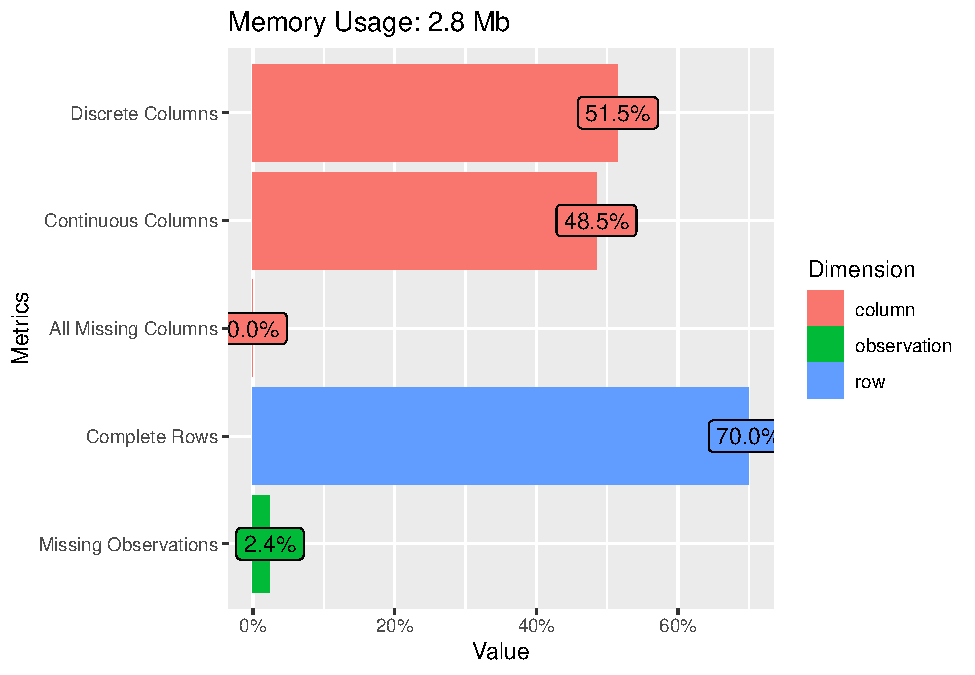
\includegraphics{_main_files/figure-latex/explore_dt_0-1.pdf}

\begin{Shaded}
\begin{Highlighting}[]
\CommentTok{\# plots percentages missing across variables}
\FunctionTok{plot\_missing}\NormalTok{(data\_nba, }\AttributeTok{missing\_only =} \ConstantTok{TRUE}\NormalTok{)}
\end{Highlighting}
\end{Shaded}

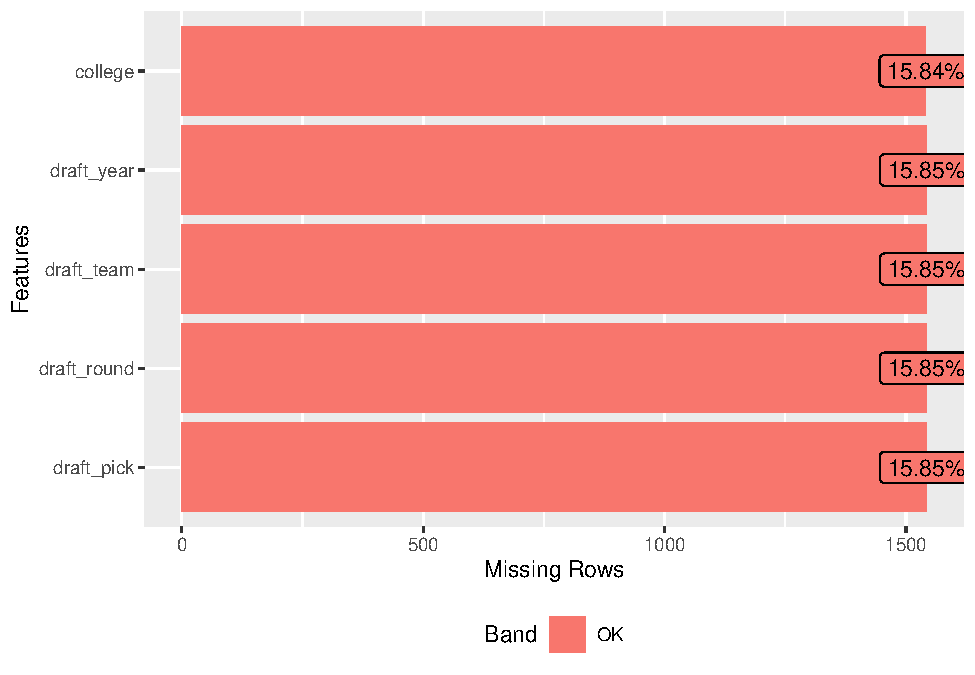
\includegraphics{_main_files/figure-latex/explore_dt_0-2.pdf}

\begin{Shaded}
\begin{Highlighting}[]
\CommentTok{\# plots frequencies across variables (here for a selected subset)}
\NormalTok{data\_nba }\SpecialCharTok{\%\textgreater{}\%} 
  \FunctionTok{select}\NormalTok{(shoots, }\FunctionTok{contains}\NormalTok{(}\StringTok{"position"}\NormalTok{)) }\SpecialCharTok{\%\textgreater{}\%} 
  \FunctionTok{plot\_bar}\NormalTok{()}
\end{Highlighting}
\end{Shaded}

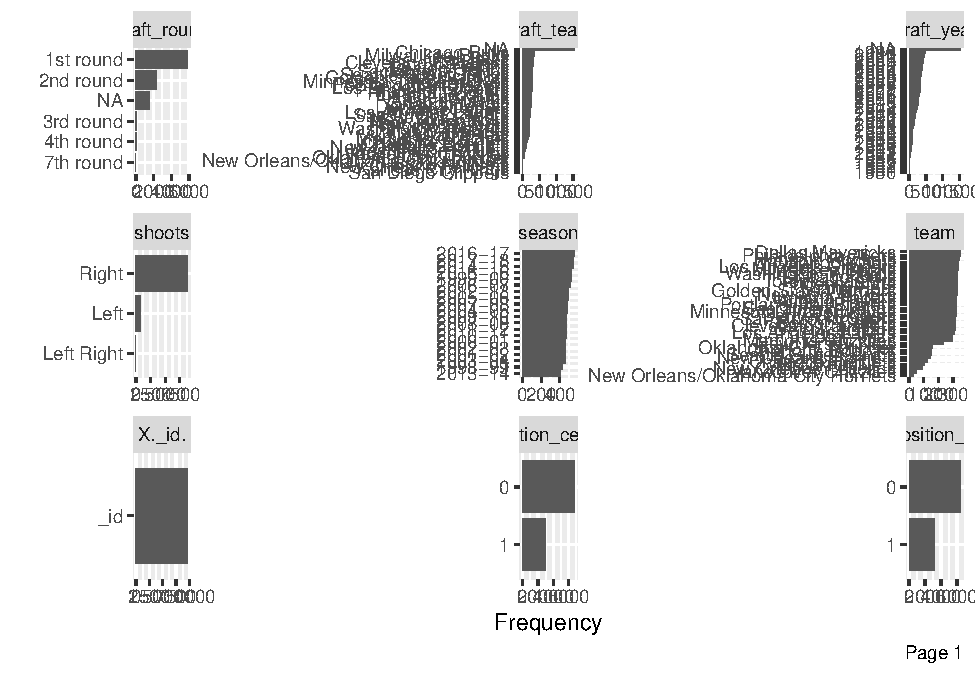
\includegraphics{_main_files/figure-latex/explore_dt_0-3.pdf}

Now, let us try \texttt{gtSummary} for summary tables. A summary table is always a useful start, once you have identified the variables you are interested in.

Let us assume we are interested in \texttt{age}, \texttt{seasons\_played}, \texttt{shoots} (shooting hand), \texttt{career\_PTS} (career points), \texttt{salary} and \texttt{position}.

\begin{Shaded}
\begin{Highlighting}[]
\FunctionTok{library}\NormalTok{(gtsummary)}

\NormalTok{data\_nba }\SpecialCharTok{\%\textgreater{}\%} 
  \FunctionTok{select}\NormalTok{(age, seasons\_played, shoots, career\_PTS, salary, }\FunctionTok{contains}\NormalTok{(}\StringTok{"position"}\NormalTok{)) }\SpecialCharTok{\%\textgreater{}\%}
         \FunctionTok{tbl\_summary}\NormalTok{(}
           \AttributeTok{statistic =} \FunctionTok{all\_continuous}\NormalTok{() }\SpecialCharTok{\textasciitilde{}} \FunctionTok{c}\NormalTok{(}\StringTok{"\{mean\} (\{min\}, \{max\})"}\NormalTok{)) }
\end{Highlighting}
\end{Shaded}

\begin{tabular}{l|c}
\hline
**Characteristic** & **N = 9,728**\\
\hline
age & 27.0 (18.0, 42.0)\\
\hline
seasons\_played & 9 (1, 21)\\
\hline
shoots & \\
\hline
Left & 856 (8.8\%)\\
\hline
Left Right & 7 (<0.1\%)\\
\hline
Right & 8,865 (91\%)\\
\hline
career\_PTS & 8.9 (0.0, 30.1)\\
\hline
salary & 4,072,633 (2,706, 34,682,550)\\
\hline
position\_center & 2,986 (31\%)\\
\hline
position\_sf & 3,222 (33\%)\\
\hline
position\_pf & 3,501 (36\%)\\
\hline
position\_sg & 3,447 (35\%)\\
\hline
position\_pg & 2,489 (26\%)\\
\hline
\end{tabular}

To explore correlations between all numeric variables in the data set, we can inspect the \emph{correlation matrix} or plot it.

\begin{Shaded}
\begin{Highlighting}[]
\CommentTok{\# selct only numeric variables and remove missing values}
\NormalTok{data\_nba\_numeric }\OtherTok{\textless{}{-}}\NormalTok{ data\_nba }\SpecialCharTok{\%\textgreater{}\%}
  \FunctionTok{select}\NormalTok{(}\FunctionTok{where}\NormalTok{(is.numeric)) }\SpecialCharTok{\%\textgreater{}\%}
  \FunctionTok{na.omit}\NormalTok{()}

\CommentTok{\# as a matrix using the corrr package}
\FunctionTok{library}\NormalTok{(}\StringTok{"corrr"}\NormalTok{)}

\NormalTok{corrmatrix }\OtherTok{\textless{}{-}}\NormalTok{ data\_nba\_numeric }\SpecialCharTok{\%\textgreater{}\%}
  \FunctionTok{correlate}\NormalTok{() }\SpecialCharTok{\%\textgreater{}\%} \CommentTok{\# create correlation data frame (cor\_df)}
  \FunctionTok{rearrange}\NormalTok{() }\SpecialCharTok{\%\textgreater{}\%} \CommentTok{\# rearrange by correlations}
  \FunctionTok{shave}\NormalTok{() }\CommentTok{\# remove the upper triangle of the matrix}

\FunctionTok{fashion}\NormalTok{(corrmatrix) }\CommentTok{\# gives a clean display of the matrix}
\end{Highlighting}
\end{Shaded}

\begin{verbatim}
##               term career_AST position_pg career_PTS career_G career_WS
## 1       career_AST                                                     
## 2      position_pg        .61                                          
## 3       career_PTS        .61         .08                              
## 4         career_G        .47         .04        .65                   
## 5        career_WS        .52        -.01        .76      .83          
## 6   seasons_played        .33         .04        .48      .79       .61
## 7      position_sg        .19         .22        .12      .09       .01
## 8           salary        .35        -.04        .60      .48       .59
## 9              age        .18         .03        .18      .49       .36
## 10     position_sf       -.08        -.33        .12      .13       .07
## 11      season_end        .01         .01        .04     -.17      -.09
## 12    season_start        .01         .01        .04     -.17      -.09
## 13          height       -.31        -.46       -.01     -.02      -.00
## 14     position_pf       -.29        -.44        .01      .11       .12
## 15 position_center       -.36        -.39       -.10      .04       .08
## 16          weight       -.49        -.66       -.06     -.03       .05
##    seasons_played position_sg salary  age position_sf season_end season_start
## 1                                                                            
## 2                                                                            
## 3                                                                            
## 4                                                                            
## 5                                                                            
## 6                                                                            
## 7             .09                                                            
## 8             .41        -.03                                                
## 9             .26         .03    .25                                         
## 10            .12         .18    .03  .03                                    
## 11            .00         .02    .16 -.07        -.04                        
## 12            .00         .02    .16 -.07        -.04       1.00             
## 13           -.03        -.03    .03 -.04         .30        .02          .02
## 14            .12        -.46    .09  .03         .04       -.00         -.00
## 15            .07        -.49    .10  .04        -.37       -.06         -.06
## 16            .04        -.43    .12 -.07        -.01        .04          .04
##    height position_pf position_center weight
## 1                                           
## 2                                           
## 3                                           
## 4                                           
## 5                                           
## 6                                           
## 7                                           
## 8                                           
## 9                                           
## 10                                          
## 11                                          
## 12                                          
## 13                                          
## 14    .15                                   
## 15    .12         .33                       
## 16    .41         .45             .66
\end{verbatim}

\begin{Shaded}
\begin{Highlighting}[]
\CommentTok{\# or plot it using a ggplot approach}
\FunctionTok{library}\NormalTok{(}\StringTok{"ggcorrplot"}\NormalTok{)}

\NormalTok{corrmatrix }\OtherTok{\textless{}{-}} \FunctionTok{round}\NormalTok{(}\FunctionTok{cor}\NormalTok{(data\_nba\_numeric), }\DecValTok{1}\NormalTok{) }\CommentTok{\# create correlation matrix}

\FunctionTok{ggcorrplot}\NormalTok{(corrmatrix,}
           \AttributeTok{method =} \StringTok{"circle"}\NormalTok{,}
           \AttributeTok{type=}\StringTok{"lower"}\NormalTok{) }\CommentTok{\# plots the matrix}
\end{Highlighting}
\end{Shaded}

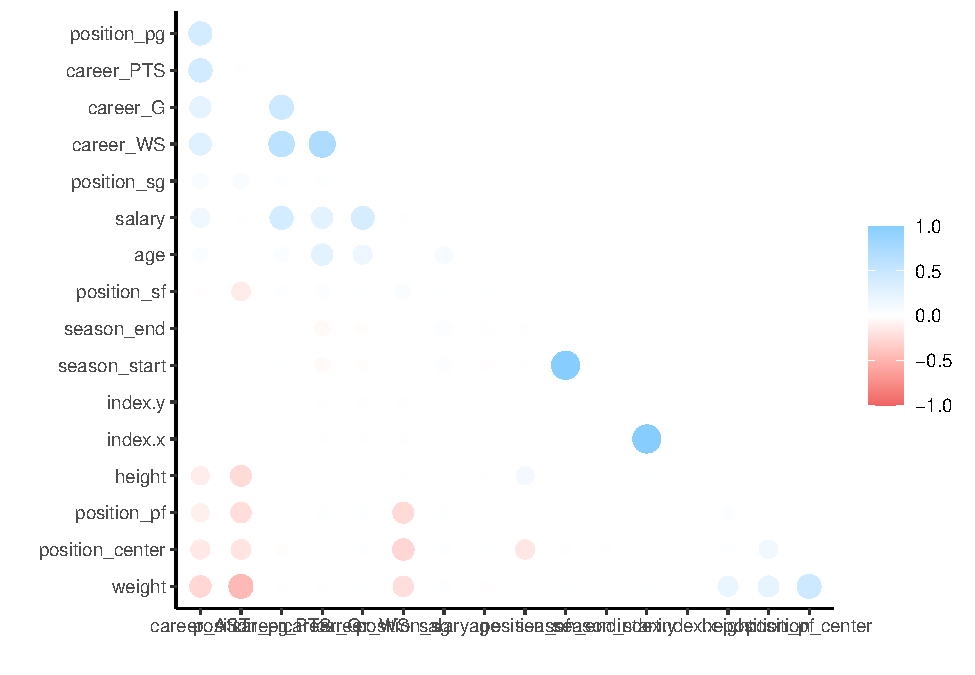
\includegraphics{_main_files/figure-latex/explore_dt_2-1.pdf}

This is interesting. For example, it seems that the weight is strongly correlated with the position a player occupies. Centers are heavy, point guards are light weights. We also see that most performance metrics (\texttt{career\_*}) are correlated with each other and also with salary. Good players seem to be good in many things, and good players seem to be paid more.

\hypertarget{explore-individual-variables}{%
\section{Explore individual variables}\label{explore-individual-variables}}

Now that we have a feeling for the whole data set, we want to explore individual variables. To keep it focused, we will follow up on the question of whether players that perform better are also paid more, for now limiting ourselves to the relationship between the average points per game and the received salary. We will also explore if this relationship depends on the position a player occupies.

Why might the position be relevant for this? We can expect that the justification for the salary differs by the occupied position, i.e.~the role a player fills for the team. To explore this we will limit ourselves to two positions for now, point guards and centers. Point guards are really good passers. Their salary may thus depend more on enabling others to score and not so much on their own point average. Centers on the other hand will mostly be on the receiving end, transforming passes into points. For them their salary may more strongly depend on the actual points they are able to score. This clearly still is an oversimplification of how basketball works but may be a first avenue to approach the relationship between salary and point average.

Let us first build a new variable that discerns between centers, point guards and all other positions and that is easier to work with when comparing the distributions. As we have seen above, there are players that play several positions. We should first check if there are centers who are also point guards, and vice versa. For simple cross tabulations, we can use the base R function \texttt{table()}.

\begin{Shaded}
\begin{Highlighting}[]
\FunctionTok{table}\NormalTok{(data\_nba}\SpecialCharTok{$}\NormalTok{position\_center, data\_nba}\SpecialCharTok{$}\NormalTok{position\_pg)}
\end{Highlighting}
\end{Shaded}

\begin{verbatim}
##    
##        0    1
##   0 4253 2489
##   1 2986    0
\end{verbatim}

We can see that there are \(0\) observations for which both variables equal \(1\). This saves us some headaches and we can construct the new variable in a straightforward way.

\begin{Shaded}
\begin{Highlighting}[]
\NormalTok{data\_nba }\OtherTok{\textless{}{-}}\NormalTok{ data\_nba }\SpecialCharTok{\%\textgreater{}\%} 
  \FunctionTok{mutate}\NormalTok{(}\AttributeTok{role =} \FunctionTok{case\_when}\NormalTok{(}
\NormalTok{    position\_pg }\SpecialCharTok{==} \DecValTok{1} \SpecialCharTok{\textasciitilde{}} \StringTok{"pg"}\NormalTok{,}
\NormalTok{    position\_center }\SpecialCharTok{==} \DecValTok{1} \SpecialCharTok{\textasciitilde{}} \StringTok{"center"}\NormalTok{,}
    \ConstantTok{TRUE} \SpecialCharTok{\textasciitilde{}} \StringTok{"other"}
\NormalTok{  ))}
\end{Highlighting}
\end{Shaded}

Let us start with the \texttt{salary} variable. There are several possible approaches to exploring the distributions of our variables of interest. We could for one use functions like \texttt{skim()} or \texttt{summary()}, but we can also construct a table with some summary statistics of interest ourselves using \texttt{summarise()}.

\begin{Shaded}
\begin{Highlighting}[]
\NormalTok{data\_nba }\SpecialCharTok{\%\textgreater{}\%} 
  \FunctionTok{summarise}\NormalTok{(}\AttributeTok{min =} \FunctionTok{min}\NormalTok{(salary),}
            \AttributeTok{p25 =} \FunctionTok{quantile}\NormalTok{(salary, }\AttributeTok{probs =} \FloatTok{0.25}\NormalTok{),}
            \AttributeTok{median =} \FunctionTok{median}\NormalTok{(salary),}
            \AttributeTok{mean =} \FunctionTok{mean}\NormalTok{(salary),}
            \AttributeTok{p75 =} \FunctionTok{quantile}\NormalTok{(salary, }\AttributeTok{probs =} \FloatTok{0.75}\NormalTok{),}
            \AttributeTok{max =} \FunctionTok{max}\NormalTok{(salary)}
\NormalTok{            )}
\end{Highlighting}
\end{Shaded}

\begin{verbatim}
## # A tibble: 1 x 6
##     min    p25  median     mean     p75      max
##   <dbl>  <dbl>   <dbl>    <dbl>   <dbl>    <dbl>
## 1  2706 947907 2240000 4072633. 5408700 34682550
\end{verbatim}

This already gives us some indication on the distribution of the variable but we may ease the interpretation using plots.

\begin{Shaded}
\begin{Highlighting}[]
\CommentTok{\# using a boxplot}
\NormalTok{data\_nba }\SpecialCharTok{\%\textgreater{}\%}
  \FunctionTok{ggplot}\NormalTok{(}\FunctionTok{aes}\NormalTok{(}\AttributeTok{x =}\NormalTok{ salary)) }\SpecialCharTok{+}
  \FunctionTok{geom\_boxplot}\NormalTok{()}
\end{Highlighting}
\end{Shaded}

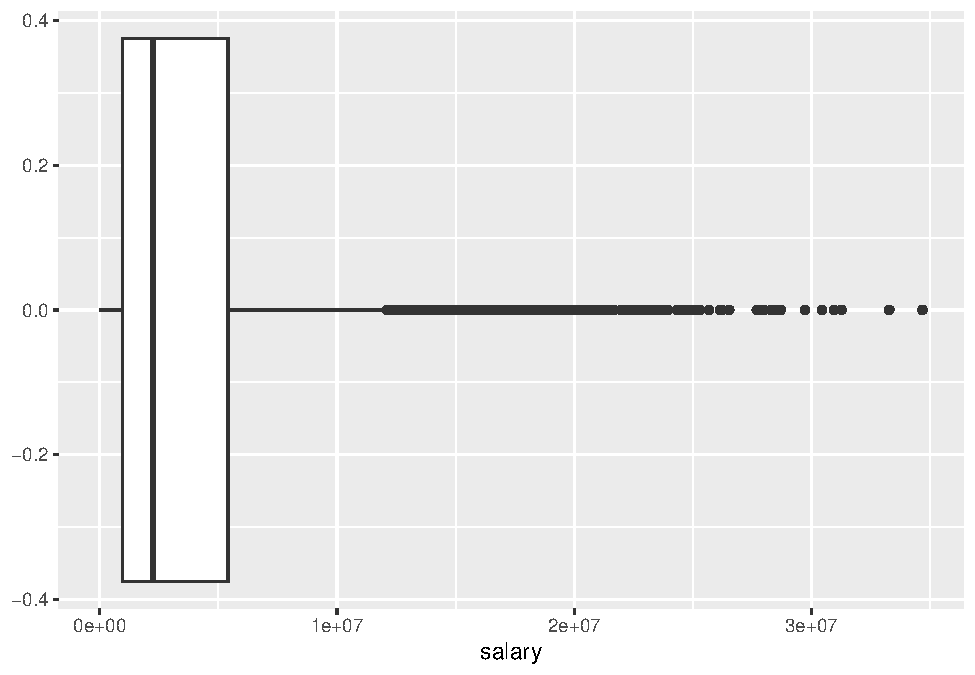
\includegraphics{_main_files/figure-latex/plot_distribution_salary-1.pdf}

\begin{Shaded}
\begin{Highlighting}[]
\CommentTok{\# using a histogram}
\NormalTok{data\_nba }\SpecialCharTok{\%\textgreater{}\%}
  \FunctionTok{ggplot}\NormalTok{(}\FunctionTok{aes}\NormalTok{(}\AttributeTok{x =}\NormalTok{ salary)) }\SpecialCharTok{+}
  \FunctionTok{geom\_histogram}\NormalTok{(}\AttributeTok{bins =} \DecValTok{50}\NormalTok{)}
\end{Highlighting}
\end{Shaded}

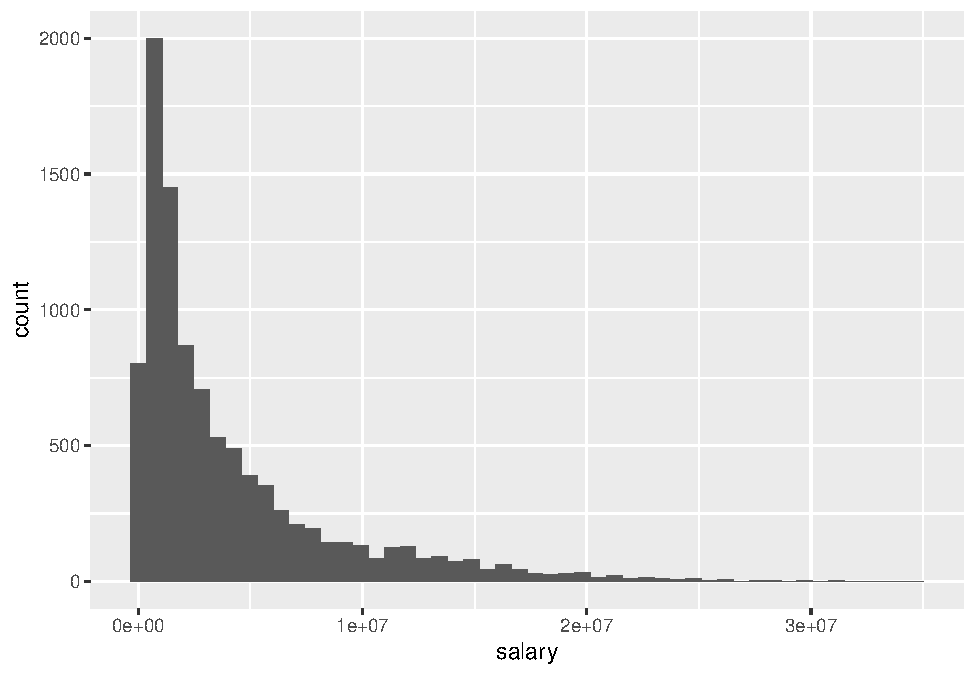
\includegraphics{_main_files/figure-latex/plot_distribution_salary-2.pdf}

\begin{Shaded}
\begin{Highlighting}[]
\CommentTok{\# using a density plot}
\NormalTok{data\_nba }\SpecialCharTok{\%\textgreater{}\%}
  \FunctionTok{ggplot}\NormalTok{(}\FunctionTok{aes}\NormalTok{(}\AttributeTok{x =}\NormalTok{ salary)) }\SpecialCharTok{+}
  \FunctionTok{geom\_density}\NormalTok{()}
\end{Highlighting}
\end{Shaded}

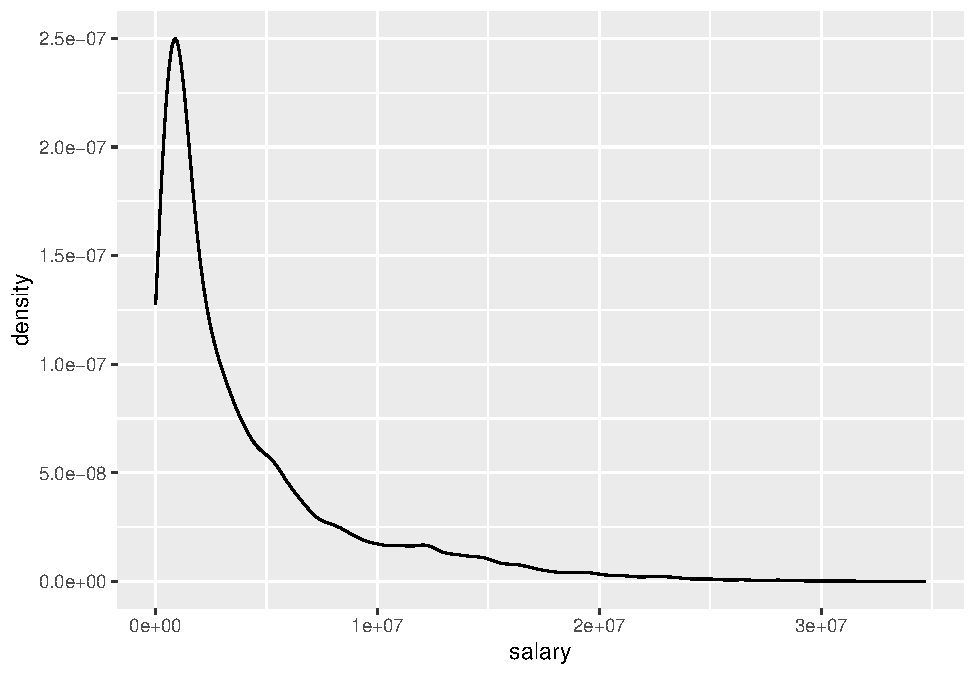
\includegraphics{_main_files/figure-latex/plot_distribution_salary-3.pdf}

The different approaches to visualizing the distribution for \texttt{salary} basically show us the same thing, the distribution is heavily skewed as we see many players with comparably modest salaries and increasingly few with very high compensations. We should keep this in mind when we turn to building a regression model.

We can also compute and visualize the distribution by the role a player fills. Using \texttt{summarise()} with \texttt{group\_by()} enables us to get the same measurements as above, but separately for each category of \texttt{role}.

\begin{Shaded}
\begin{Highlighting}[]
\NormalTok{data\_nba }\SpecialCharTok{\%\textgreater{}\%} 
  \FunctionTok{group\_by}\NormalTok{(role) }\SpecialCharTok{\%\textgreater{}\%} 
  \FunctionTok{summarise}\NormalTok{(}\AttributeTok{min =} \FunctionTok{min}\NormalTok{(salary),}
            \AttributeTok{p25 =} \FunctionTok{quantile}\NormalTok{(salary, }\AttributeTok{probs =} \FloatTok{0.25}\NormalTok{),}
            \AttributeTok{median =} \FunctionTok{median}\NormalTok{(salary),}
            \AttributeTok{mean =} \FunctionTok{mean}\NormalTok{(salary),}
            \AttributeTok{p75 =} \FunctionTok{quantile}\NormalTok{(salary, }\AttributeTok{probs =} \FloatTok{0.75}\NormalTok{),}
            \AttributeTok{max =} \FunctionTok{max}\NormalTok{(salary)}
\NormalTok{            )}
\end{Highlighting}
\end{Shaded}

\begin{verbatim}
## # A tibble: 3 x 7
##   role     min     p25  median     mean     p75      max
##   <chr>  <dbl>   <dbl>   <dbl>    <dbl>   <dbl>    <dbl>
## 1 center  4529 1115340 2880000 4770707. 6400000 28000000
## 2 other   2706  863640 2000000 3757860. 5000000 33285709
## 3 pg      2853  895248 2100000 3773028. 5000000 34682550
\end{verbatim}

For plotting by role, let us limit ourselves to boxplots.

\begin{Shaded}
\begin{Highlighting}[]
\NormalTok{data\_nba }\SpecialCharTok{\%\textgreater{}\%}
  \FunctionTok{ggplot}\NormalTok{(}\FunctionTok{aes}\NormalTok{(}\AttributeTok{x =}\NormalTok{ salary, }\AttributeTok{colour =}\NormalTok{ role)) }\SpecialCharTok{+}
  \FunctionTok{geom\_boxplot}\NormalTok{()}
\end{Highlighting}
\end{Shaded}

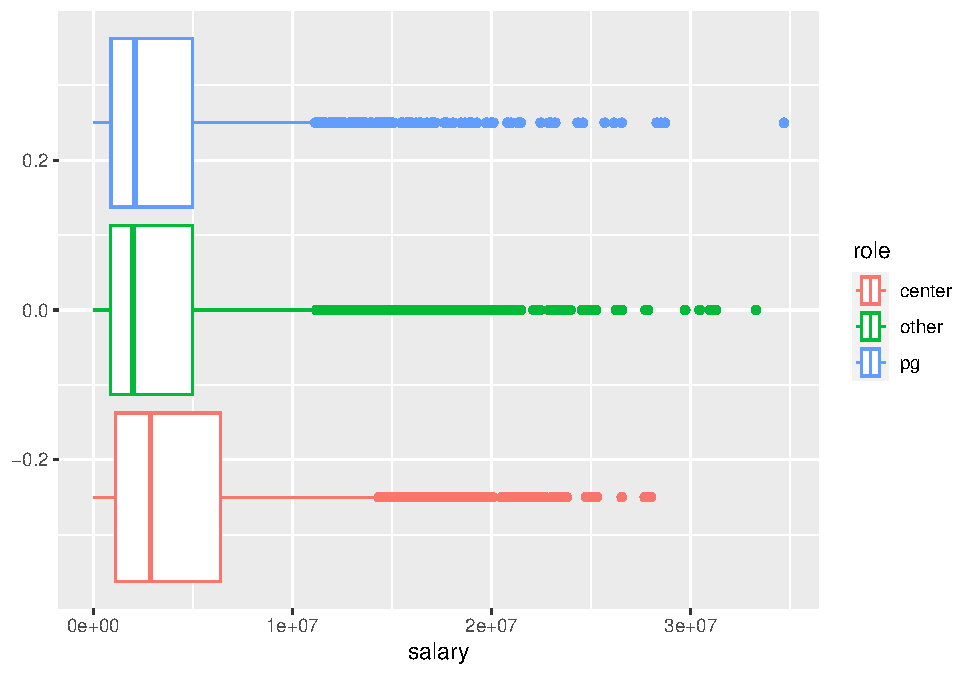
\includegraphics{_main_files/figure-latex/plot_distribution_salary_role-1.pdf}

We can see, that while point guards barely differ from their peers, centers do. The average salary for centers is higher compared to all other roles. At the same time while many of them reach very high salaries, the top earner spots are reserved for other roles. The highest earning point guard makes almost \(6,700,000\$\) more compared to the highest earning center; a substantial difference. As the boxplot indicates, the players with such extreme salaries are also in the extreme minority so we should not over interpret this finding. Still, the puzzle seems to be more complex than we thought.

Let us turn to \texttt{career\_PTS} now and repeat the analysis from above.

\begin{Shaded}
\begin{Highlighting}[]
\NormalTok{data\_nba }\SpecialCharTok{\%\textgreater{}\%} 
  \FunctionTok{summarise}\NormalTok{(}\AttributeTok{min =} \FunctionTok{min}\NormalTok{(career\_PTS),}
            \AttributeTok{p25 =} \FunctionTok{quantile}\NormalTok{(career\_PTS, }\AttributeTok{probs =} \FloatTok{0.25}\NormalTok{),}
            \AttributeTok{median =} \FunctionTok{median}\NormalTok{(career\_PTS),}
            \AttributeTok{mean =} \FunctionTok{mean}\NormalTok{(career\_PTS),}
            \AttributeTok{p75 =} \FunctionTok{quantile}\NormalTok{(career\_PTS, }\AttributeTok{probs =} \FloatTok{0.75}\NormalTok{),}
            \AttributeTok{max =} \FunctionTok{max}\NormalTok{(career\_PTS)}
\NormalTok{            )}
\end{Highlighting}
\end{Shaded}

\begin{verbatim}
## # A tibble: 1 x 6
##     min   p25 median  mean   p75   max
##   <dbl> <dbl>  <dbl> <dbl> <dbl> <dbl>
## 1     0   5.1      8  8.91    12  30.1
\end{verbatim}

\begin{Shaded}
\begin{Highlighting}[]
\NormalTok{data\_nba }\SpecialCharTok{\%\textgreater{}\%}
  \FunctionTok{ggplot}\NormalTok{(}\FunctionTok{aes}\NormalTok{(}\AttributeTok{x =}\NormalTok{ career\_PTS)) }\SpecialCharTok{+}
  \FunctionTok{geom\_boxplot}\NormalTok{()}
\end{Highlighting}
\end{Shaded}

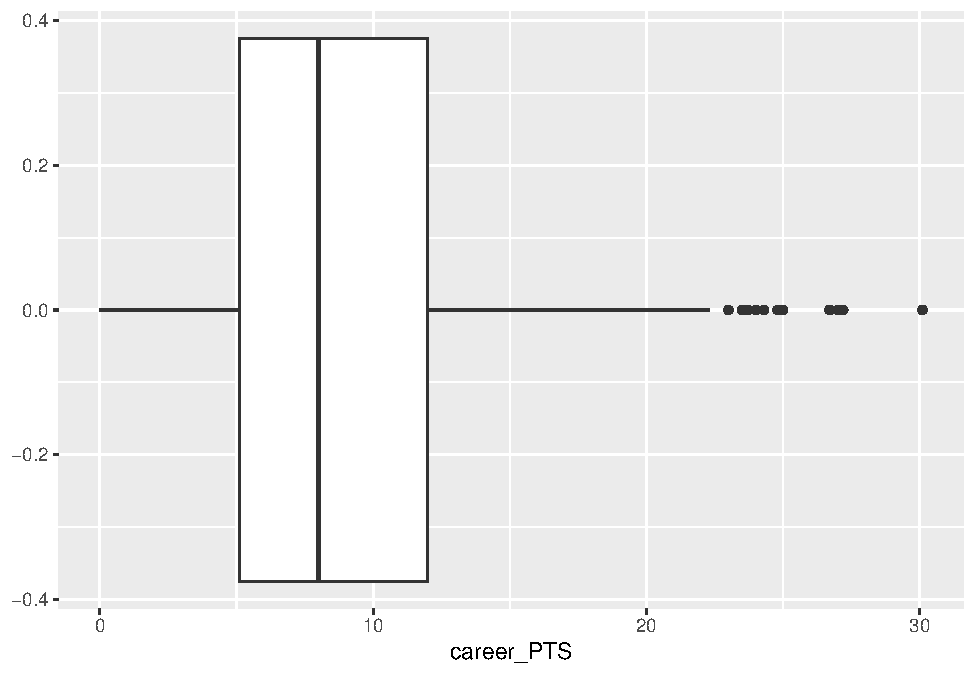
\includegraphics{_main_files/figure-latex/summarise_distribution_points-1.pdf}

\begin{Shaded}
\begin{Highlighting}[]
\NormalTok{data\_nba }\SpecialCharTok{\%\textgreater{}\%}
  \FunctionTok{ggplot}\NormalTok{(}\FunctionTok{aes}\NormalTok{(}\AttributeTok{x =}\NormalTok{ career\_PTS)) }\SpecialCharTok{+}
  \FunctionTok{geom\_histogram}\NormalTok{(}\AttributeTok{bins =} \DecValTok{50}\NormalTok{)}
\end{Highlighting}
\end{Shaded}

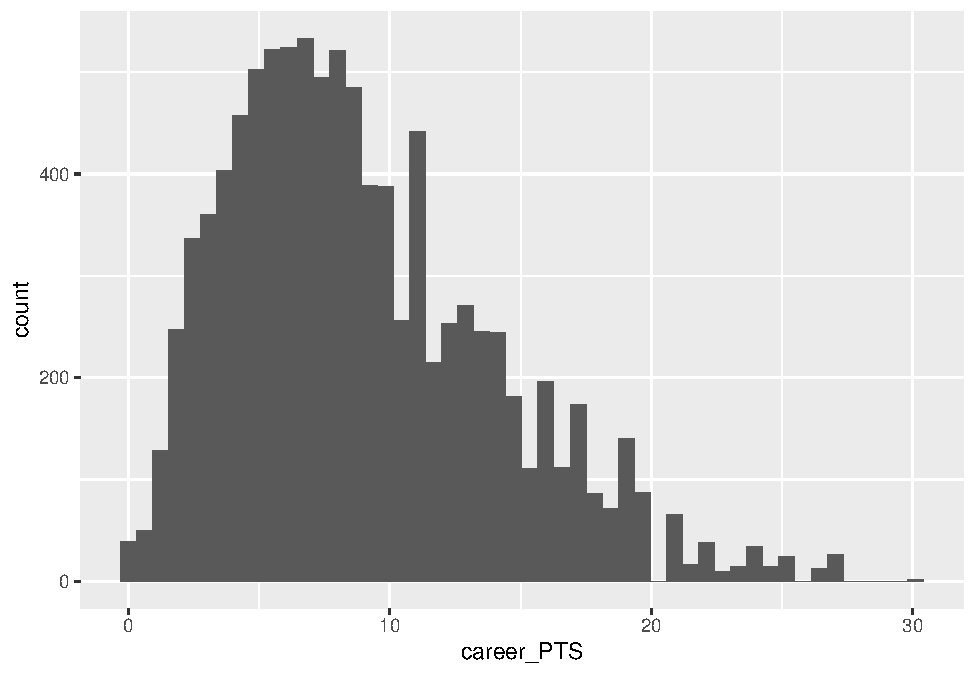
\includegraphics{_main_files/figure-latex/summarise_distribution_points-2.pdf}

While the distribution of average career points is also somewhat skewed, it is way less so compared to \texttt{salary}.

We should also look at \texttt{career\_PTS} by role.

\begin{Shaded}
\begin{Highlighting}[]
\NormalTok{data\_nba }\SpecialCharTok{\%\textgreater{}\%} 
  \FunctionTok{group\_by}\NormalTok{(role) }\SpecialCharTok{\%\textgreater{}\%} 
  \FunctionTok{summarise}\NormalTok{(}\AttributeTok{min =} \FunctionTok{min}\NormalTok{(career\_PTS),}
            \AttributeTok{p25 =} \FunctionTok{quantile}\NormalTok{(career\_PTS, }\AttributeTok{probs =} \FloatTok{0.25}\NormalTok{),}
            \AttributeTok{median =} \FunctionTok{median}\NormalTok{(career\_PTS),}
            \AttributeTok{mean =} \FunctionTok{mean}\NormalTok{(career\_PTS),}
            \AttributeTok{p75 =} \FunctionTok{quantile}\NormalTok{(career\_PTS, }\AttributeTok{probs =} \FloatTok{0.75}\NormalTok{),}
            \AttributeTok{max =} \FunctionTok{max}\NormalTok{(career\_PTS)}
\NormalTok{            )}
\end{Highlighting}
\end{Shaded}

\begin{verbatim}
## # A tibble: 3 x 7
##   role     min   p25 median  mean   p75   max
##   <chr>  <dbl> <dbl>  <dbl> <dbl> <dbl> <dbl>
## 1 center     0   4.5    7    8.17  11.2  24.3
## 2 other      0   5.2    8.2  9.04  12    30.1
## 3 pg         0   6.3    8.9  9.57  12.6  26.7
\end{verbatim}

\begin{Shaded}
\begin{Highlighting}[]
\NormalTok{data\_nba }\SpecialCharTok{\%\textgreater{}\%}
  \FunctionTok{ggplot}\NormalTok{(}\FunctionTok{aes}\NormalTok{(}\AttributeTok{x =}\NormalTok{ career\_PTS, }\AttributeTok{colour =}\NormalTok{ role)) }\SpecialCharTok{+}
  \FunctionTok{geom\_boxplot}\NormalTok{()}
\end{Highlighting}
\end{Shaded}

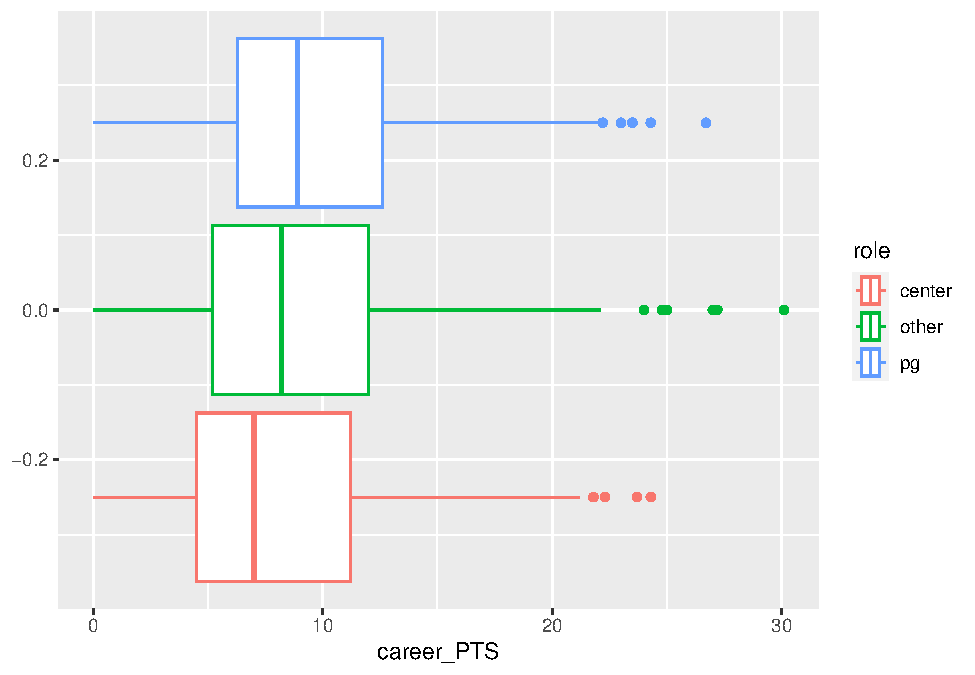
\includegraphics{_main_files/figure-latex/summarise_distribution_points_role-1.pdf}

Centers actually make less points on average compared to all other roles and point guards score the highest on average. That is an interesting puzzle to explore. It seems that point guards are paid a little less even though they make a few more points on average. What does this tell us? We can not be sure yet, but it seems that the relationship between points and salary gets translated differently based on the role a player occupies.

Let us now explore this relationship between the two variables, which will be central to our analysis from now on. We can use a scatter plot to inspect the shared distribution of both variables. We also added a line describing the relationship. This actually is a regression line and we will talk about it in detail \protect\hyperlink{lin-t-1}{later}, for now let us just accept that the direction of the line tells us how both variables are related.

\begin{Shaded}
\begin{Highlighting}[]
\NormalTok{data\_nba }\SpecialCharTok{\%\textgreater{}\%} 
  \FunctionTok{ggplot}\NormalTok{(}\FunctionTok{aes}\NormalTok{(}\AttributeTok{y =}\NormalTok{ salary, }\AttributeTok{x =}\NormalTok{ career\_PTS)) }\SpecialCharTok{+}
  \FunctionTok{geom\_point}\NormalTok{() }\SpecialCharTok{+}
  \FunctionTok{geom\_smooth}\NormalTok{(}\AttributeTok{method =} \StringTok{"lm"}\NormalTok{)}
\end{Highlighting}
\end{Shaded}

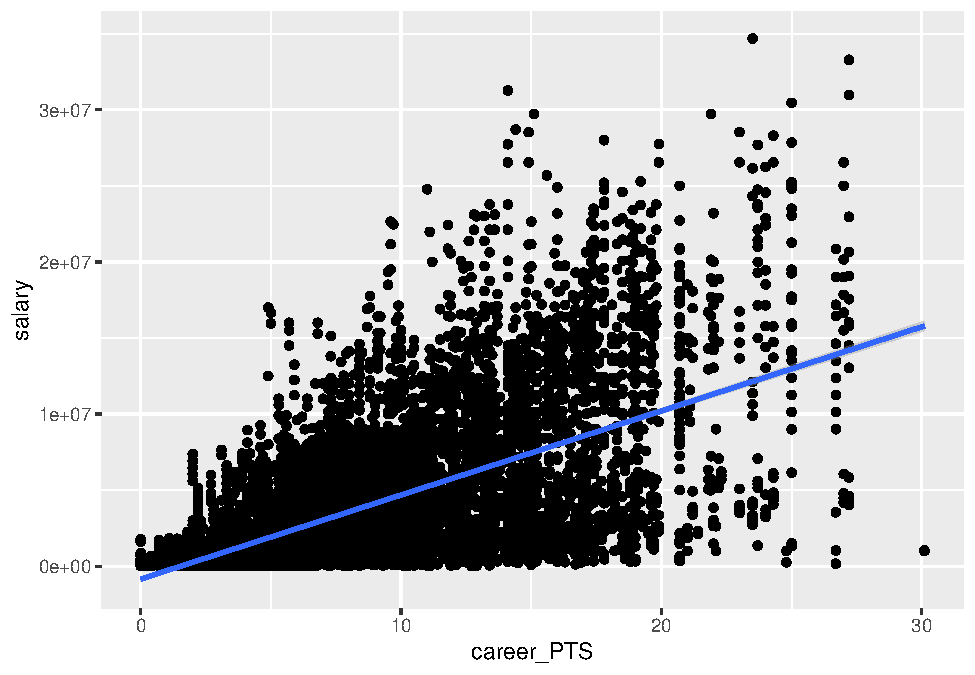
\includegraphics{_main_files/figure-latex/salary_points_scatter-1.pdf}

We can see that there is a positive relationship between the average score and the earned salary. The more points a player scores the more he earns, on average.

We can build the same plot by \texttt{role}.

\begin{Shaded}
\begin{Highlighting}[]
\NormalTok{data\_nba }\SpecialCharTok{\%\textgreater{}\%} 
  \FunctionTok{ggplot}\NormalTok{(}\FunctionTok{aes}\NormalTok{(}\AttributeTok{y =}\NormalTok{ salary, }\AttributeTok{x =}\NormalTok{ career\_PTS, }\AttributeTok{colour =}\NormalTok{ role)) }\SpecialCharTok{+}
  \FunctionTok{geom\_point}\NormalTok{(}\AttributeTok{alpha =} \FloatTok{0.25}\NormalTok{) }\SpecialCharTok{+}
  \FunctionTok{geom\_smooth}\NormalTok{(}\AttributeTok{method =} \StringTok{"lm"}\NormalTok{)}
\end{Highlighting}
\end{Shaded}

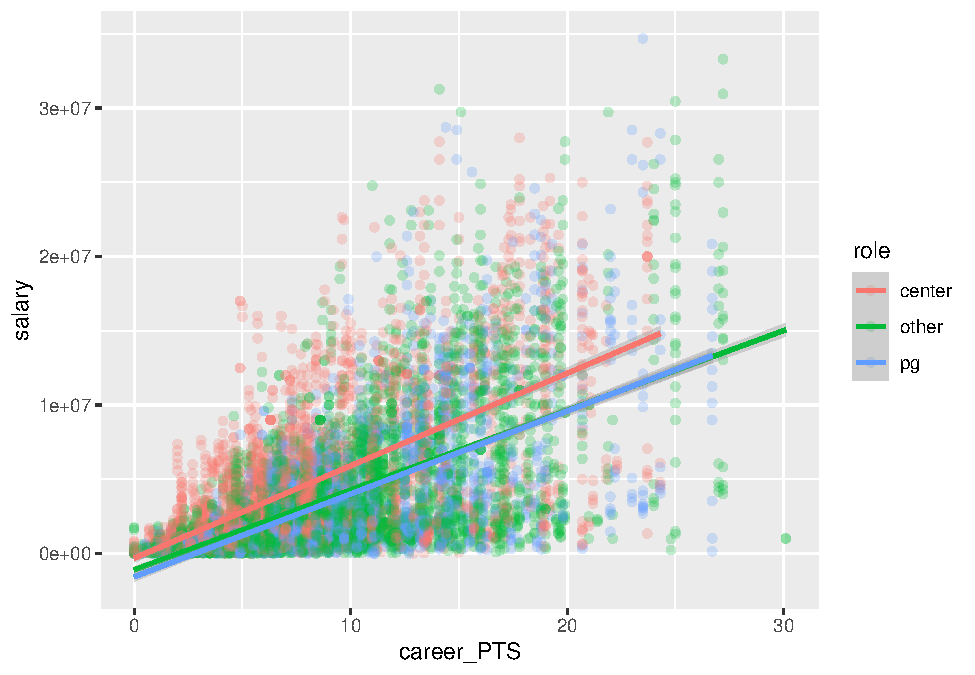
\includegraphics{_main_files/figure-latex/salary_points_role_scatter-1.pdf}

Let's reflect a moment what we can learn from all this.

First, there seems to be a somewhat linear relationship between how many points a player scores and how much they are paid. This also holds true for point guards just as much as for non-point guards. However, the average salary for point guards is lower in comparison. We also learn that the link between salary and points is stronger for centers as the red line is somewhat steeper. They seem to be paid more, the more they score.

\hypertarget{moving-on}{%
\section{Moving on}\label{moving-on}}

We have now explored our data and gained a better understanding of the variables of interest. We also have identified an interesting puzzle to explre further, and we will pick up on this over the seminar. In \protect\hyperlink{dags-1}{week 4}, we will construct a theoretical model that tries to explain the relationship between points and salary and in \protect\hyperlink{lin-a}{week 8} we will then compute a linear regression model that will hopefully shed some more light on our puzzle. Linear regression is all about further exploring the relationship between two or more variables, one outcome (often called \texttt{y}) and one or multiple independent variables (often called \texttt{x}). Independent variables have many names. They are sometimes called ``covariates''; ``predictors''; ``exposure'', depending on the context.

There are a number of cool things that regression can do for us that simple EDA cannot:

\begin{enumerate}
\def\labelenumi{\arabic{enumi})}
\item
  It can model the relationship between two variables while considering simultaneously the potential influence of other factors. Imagine we are interested in the effect of points per game on salary regardless of position, season, team or other independent variables. With regression we can estimate how much more a player would earn every season if he scored 10 more points a game (regardless of other factors as for example the position he plays).
\item
  It can assess what explains the effect of one variable on another (i.e.~mediation). Maybe we find that point guards earn less and we want to know why. Is it because they score less? Is it because they play less time on average?
\item
  It can be used to predict salaries for players for whom we don't know the salary or even for hypothetical players. We could also look at the performance trend of players and predict whether they earn more next season or not.
\end{enumerate}

We will address all these applications over the course of the seminar.

\hypertarget{further-resources}{%
\section{Further resources}\label{further-resources}}

\begin{itemize}
\tightlist
\item
  \href{https://tuos-bio-data-skills.github.io/intro-eda-book/index.html}{Exploratory Data Analysis with R}, a book that covers the basics of data visualization, manipulation, and analysis using R and the tidyverse package.
\item
  \href{https://www.pluralsight.com/guides/exploratory-data-analysis-in-r}{Exploratory Data Analysis in R with Tidyverse}, a guide that shows how to use the tidyverse package to perform common EDA tasks such as importing, cleaning, summarizing, and plotting data.
\item
  \href{https://r4ds.had.co.nz/data-visualisation.html}{Data Visualization with ggplot2}, a chapter from the book R for Data Science that explains how to create and customize different types of plots using the ggplot2 package.
\item
  \href{https://r4ds.had.co.nz/transform.html}{Data Transformation with dplyr}, another chapter from the book R for Data Science that demonstrates how to use the dplyr package to manipulate data frames, filter rows, select columns, create new variables, and more.
\item
  \href{https://bookdown.org/rdpeng/exdata/}{Exploratory Data Analysis with R - Bookdown}
\item
  \href{https://www.statology.org/exploratory-data-analysis-in-r/}{How to Perform Exploratory Data Analysis in R (With Example)}
\end{itemize}

\hypertarget{eda-2}{%
\chapter{Exploratory Data Analysis - Exercise}\label{eda-2}}

This week we will apply the concepts from last week in an exercise where you will conduct an exploratory data analysis on a different data set. To document your work on these exercises, you will use \emph{R Markdown}.

\hypertarget{what-is-r-markdown}{%
\section{What is R Markdown?}\label{what-is-r-markdown}}

R Markdown allows you to combine written text that is easy to format with R Code that is executed when \emph{knitting} or \emph{compiling} the document into the chosen output format. This allows us to describe our research, analyse our data, display results as tables or plots and interpret these, all in one file. In this way we can not only create reports on seminar exercises but also write websites - like the one your are looking at in this very moment -, seminar papers, articles or create presentations.

It is also a great notebook for projects you are working on. More often than not, our work on a specific analysis will span multiple days, weeks or even months and it is often hard to remember what we were thinking the last time we worked on our code.

\begin{quote}
``I am sure I had my reasons for writing this piece of code, but I can not for the life of me remember any of them\ldots{}''

--- Anonymous Coder 2023
\end{quote}

If we use R Markdown to document our work we can add text that explains our reasons, thoughts, ideas and plans at that very moment and pick up our work from there the next time we open the file.

R Markdown allows output to different file formats, including \texttt{html}, \texttt{docx}, \texttt{pptx} and \texttt{pdf}. Note that you need a LaTeX installation to knit to \texttt{pdf}. LaTeX is a typesetting language and used for producing high quality \texttt{pdf} documents. For simple \texttt{pdf} reports or presentations - sidenote: if you bring a \texttt{pptx} to a talk something will most probably go wrong or stop working\ldots{} - you do not really need to know how LaTeX works, you just need an installed distribution. For these purposes the package \texttt{tinytex} gives you all you need and is easy to install from within R. \href{https://bookdown.org/yihui/rmarkdown/installation.html\#installation}{This site} explains how to install it. You can also get an overview of all possible output formats \href{https://rmarkdown.rstudio.com/lesson-9.html}{here}.

\hypertarget{creating-a-r-markdown-file}{%
\section{Creating a R Markdown file}\label{creating-a-r-markdown-file}}

Before you can create and compile R Markdown documents, you first have to install the package by writing \texttt{install.packages("rmarkdown")} in your console.

Creating a new R Markdown file is as straightforward as it can be. In RStudio you can click of \texttt{File\ \textgreater{}\ New\ File\ \textgreater{}\ R\ Markdown...}. In the new window you can set up some basic information on the document - which will be displayed in the output - and chose your desired format. You can basically write R Markdown files in any text editor, just make sure that the file extension is saved as \texttt{.Rmd}. We still recommend using RStudio because it gives you some convenient options that a text editor will not, e.g.~displaying a preview of your document and easy knitting of the final file.

\hypertarget{writing-in-r-markdown}{%
\section{Writing in R Markdown}\label{writing-in-r-markdown}}

\hypertarget{document-components}{%
\subsection{Document components}\label{document-components}}

When you followed the steps above, a new R Markdown file will have been created. It basically consists of two main parts:

\begin{itemize}
\item
  A \texttt{YAML} header - surrounded by three dashes \texttt{-\/-\/-} - where options for the document can be set. The good news is that you do not have to do anything here until you get more profound with using R Markdown. For now it is enough that all the options you set when creating the new file - the title, author, date and format of the output - are present and will be included in your output file.
\item
  A body that contains the actual content of your document. Text is directly written in the body at the location where it is to be displayed in the output. We can use the simple Markdown syntax for formatting using a set of symbols, some of which we will explain below. We can also include R code in so called \texttt{chunks}, specifying if we also want it and/or the results to be displayed or ``just'' to be executed in the background. The code chunks will be executed when we compile the final document and everything that we want to include in the output - e.g.~tables, plots or code examples - will be displayed where it occurs.
\end{itemize}

\hypertarget{formatting}{%
\subsection{Formatting}\label{formatting}}

Here are some of the more common formatting elements you will need when starting out using R Markdown:

\hypertarget{headers}{%
\subsubsection{Headers}\label{headers}}

To include sections in a document we use \texttt{\#} followed by the header we want to be displayed. We can define levels for sections by using multiple \texttt{\#} in this way:

\begin{verbatim}
# Section 1
## Section 1.1
## Section 1.2
### Section 1.2.1
### Section 1.2.2
## Section 1.3
# Section 2
\end{verbatim}

\hypertarget{text}{%
\subsubsection{Text}\label{text}}

We write the text between the section headers at the place where it should be displayed in the final document. We can insert line breaks at any point but these will not be rendered in the output. To include an actual paragraph we will have to include a blank line between between two blocks of text. Two emphasize certain words or phrases, we can wrap them in \texttt{*} for italics or \texttt{**} for bold face.

Consider this Markdown code:

\begin{verbatim}
This is the first paragraph.
This still is the first paragraph.

Here begins the second paragraph.
It includes emphasis, by using *italics* and also **bold face** words.
\end{verbatim}

It is rendered as:

This is the first paragraph. This still is the first paragraph.

Here begins the second paragraph. It includes emphasis, by using \emph{italics} and also \textbf{bold face} words.

\hypertarget{lists}{%
\subsubsection{Lists}\label{lists}}

Unordered lists or bullet points can be inserted by adding a \texttt{-}, \texttt{*} or \texttt{+} at the beginning of a line. To create levels, we have to indent lines using tab stops.

\begin{verbatim}
* Level 1
* Level 1
  * Level 2
    * Level 3
  * Level 2
    * Level 3
* Level 1
\end{verbatim}

The above will be rendered as:

\begin{itemize}
\tightlist
\item
  Level 1
\item
  Level 1

  \begin{itemize}
  \tightlist
  \item
    Level 2

    \begin{itemize}
    \tightlist
    \item
      Level 3
    \end{itemize}
  \item
    Level 2

    \begin{itemize}
    \tightlist
    \item
      Level 3
    \end{itemize}
  \end{itemize}
\item
  Level 1
\end{itemize}

We can also create ordered lists by using numbers followed by a \texttt{.} instead of the \texttt{*} etc.

\begin{verbatim}
1.  Bulletpoint 1
2.  Bulletpoint 2
3.  Bulletpoint 3
\end{verbatim}

\begin{enumerate}
\def\labelenumi{\arabic{enumi}.}
\tightlist
\item
  Bulletpoint 1
\item
  Bulletpoint 2
\item
  Bulletpoint 3
\end{enumerate}

\hypertarget{hyperlinks}{%
\subsubsection{Hyperlinks}\label{hyperlinks}}

Hyperlinks can be included as \texttt{\textless{}url\textgreater{}} or \texttt{{[}text{]}(url)}.

\begin{verbatim}
To include a plain url we can use <https://jaspertjaden.github.io/DataAnalysisR/>.
We can also [link](https://jaspertjaden.github.io/DataAnalysisR/) in this way.
\end{verbatim}

To include a plain url we can use \url{https://jaspertjaden.github.io/DataAnalysisR/}. We can also \href{https://jaspertjaden.github.io/DataAnalysisR/}{link} in this way.

\hypertarget{code-chunks}{%
\subsection{Code chunks}\label{code-chunks}}

Codechunks have to be started and ended with three backticks \texttt{\textasciigrave{}\textasciigrave{}\textasciigrave{}}. After the first set of backticks we also have to include \texttt{\{r\}} to let Markdown know that we want to run the code as R code. The code that is written after this and up to the second set of backticks will be executed when knitting the file.

You can see some examples of this in the newly created R Markdown file if you followed the steps above.

We can also always run the code in a chunk before knitting by clicking on the green arrow in the upper right corner of the chunk. We can also execute individual lines of code by placing our keyboard cursor in the line and pressing \texttt{Shift\ +\ Enter}.

\hypertarget{chunk-options}{%
\subsubsection{Chunk options}\label{chunk-options}}

We can change the way code chunks are handled when knitting by adding one or multiple chunk options between the curly brackets like this: \texttt{\{r\ option=value\}}. If we want to use multiple options they have to be written like this: \texttt{\{r\ option1=value1,\ option2=value2\}}.

There are many options available but most are not needed when starting out. The ones that may be of interest to you are:

\begin{itemize}
\tightlist
\item
  \texttt{\{r\ echo=FALSE\}}: This prevents the code to be displayed in the output while the results will be included. This is useful if you want to show the results of a computation or a plot but do not want the document to be cluttered with the underlying code.
\item
  \texttt{\{r\ include=FALSE\}}: This prevents the code as well as the output from being displayed. The code is still run in the background.
\item
  \texttt{\{r\ eval=FALSE\}}: This prevents the code from being run but displays it. This can be useful if you want to show code examples for illustrative purposes.
\end{itemize}

\hypertarget{further-resources-1}{%
\section{Further resources}\label{further-resources-1}}

\begin{itemize}
\tightlist
\item
  \href{https://rmarkdown.rstudio.com/lesson-1.html}{R Markdown Website by RStudio}: A comprehensive introduction to using R Markdown from within RStudio
\item
  \href{https://bookdown.org/yihui/rmarkdown/}{Yihui Xie, J. J. Allaire, Garrett Grolemund. R Markdown: The Definitive Guide}: An in-depth overview over basically everything R Markdown can do
\item
  \href{https://rstudio.github.io/cheatsheets/rmarkdown.pdf}{R Markdown Cheat Sheet}: A cheat sheet for R Markdown, those are always helpful
\end{itemize}

\hypertarget{eda---exercise}{%
\section{EDA - Exercise}\label{eda---exercise}}

In this and all following exercises, we will work with the \textbf{Boston Housing Data}. The data set contains information on 506 census tracts in the US city of Boston from the 1970 census. It contains information on the median value of owner-occupied homes and additional statistics on houses and socio-demographics for each tract.

This is an overview of all variables included in the data set:

\begin{verbatim}
1. crim - per capita crime rate by town
2. zn - proportion of residential land zoned for lots over 25,000 sq.ft.
3. indus - proportion of non-retail business acres per town.
4. chas - Charles River dummy variable (1 if tract bounds river; 0 otherwise)
5. nox - nitric oxides concentration (parts per 10 million)
6. rm - average number of rooms per dwelling
7. age - proportion of owner-occupied units built prior to 1940
8. dis - weighted distances to five Boston employment centres
9. rad - index of accessibility to radial highways
10. tax - full-value property-tax rate per $10,000
11. ptratio - pupil-teacher ratio by town
12. b - 1000(Bk - 0.63)^2 where Bk is the proportion of blacks by town
13. lstat - % of lower status of the population
14. medv - Median value of owner-occupied homes in $1000's
\end{verbatim}

For more information on the data set and its implementation in \texttt{mlbench} please follow this \href{https://search.r-project.org/CRAN/refmans/mlbench/html/BostonHousing.html}{link}.

\begin{enumerate}
\def\labelenumi{\arabic{enumi}.}
\item
  \textbf{Prepare your R Markdown File}: Create a new R Markdown file setting the output format to \texttt{html} or \texttt{pdf} (if you have a LaTeX distribution installed) and setting the title, author and date to appropriate values. Remove the sample text and code chunks taking care to not remove the \texttt{YAML} header. Write all solutions in this file using code chunks as well as text to structure the file (headers) and answer the questions. Do not forget to save the file in the format \texttt{your\_name\_exercise\_1.Rmd}. You will have to turn in this file to the lecturers through Moodle.
\item
  \textbf{Import the dataset}: Import the data set by using the code below. The package \texttt{mlbench} conveniently includes the data set. You have to install the package beforehand by writing: \texttt{install.packages("mlbench")}. You should also load the \texttt{tidyverse} package to ease the further analysis. Not that this code also has to be included in your R Markdown file.
\end{enumerate}

\begin{Shaded}
\begin{Highlighting}[]
\FunctionTok{library}\NormalTok{(mlbench)}
\FunctionTok{library}\NormalTok{(tidyverse)}

\FunctionTok{data}\NormalTok{(BostonHousing)}
\end{Highlighting}
\end{Shaded}

\begin{enumerate}
\def\labelenumi{\arabic{enumi}.}
\setcounter{enumi}{2}
\item
  \textbf{Inspect the dataset}: Use the proper functions to inspect the structure and contents of the data set. How many categorical variables are there? How many numerical variables are there? Are there any missing values?
\item
  \textbf{Summarize categorical variables}: Create a frequency table for the categorical variable \texttt{chas} (Charles River dummy variable).
\item
  \textbf{Summarize numerical variables}: Generate summary statistics for the numerical variables crim (per capita crime rate by town), rm (average number of rooms per dwelling) and dis (weighted distances to five Boston employment centres).
\item
  \textbf{Create new variables}: Create a new variable that groups houses by their proximity to employment centers as indicated in the variable \texttt{dis}. Create the three categories \texttt{Near}, \texttt{Medium} and \texttt{Far} based on the value of \texttt{dis}. Choose appropriate cutoff values based on the summary statistics you computed above. Briefly describe your decision.
\item
  \textbf{Compare distributions}: Compare the distribution of \texttt{ptratio} by the newly created variable \texttt{distance\_group} using boxplots. Briefly interpret the results.
\item
  \textbf{Visualize relationships}: Create scatter plots with an added regression line to explore the relationship between housing prices (\texttt{medv}) and the numeric variables : \texttt{rm}, \texttt{age}, \texttt{dis}, \texttt{lstat}. Briefly interpret the plots.
\item
  \textbf{Correlation analysis}: Calculate correlation coefficients between housing prices (\texttt{medv}), the average number of rooms per dwelling (\texttt{rm}) and the crime rate (\texttt{crim}). Display the correlations as a matrix or as a plot. Interpret the result.
\end{enumerate}

\hypertarget{dags-1}{%
\chapter{DAGs}\label{dags-1}}

\hypertarget{objectives-1}{%
\section{Objectives}\label{objectives-1}}

\begin{itemize}
\tightlist
\item
  Getting to know DAGs
\item
  Understand its implications on achieving unbiased estimates for
  effects of interest
\item
  Building a DAG for the NBA data to model the effect of scored points
  on salary
\end{itemize}

\hypertarget{functions-covered}{%
\section{Functions Covered}\label{functions-covered}}

\begin{itemize}
\tightlist
\item
  \texttt{dagitty()}: Define Directed Acyclic Graphs.
\item
  \texttt{plot()}: A generic base R function that can be used to plot a DAG.
\item
  \texttt{adjustmentSets()}: Derive the adjustment set from a DAG.
\end{itemize}

\hypertarget{modelling}{%
\section{Modelling}\label{modelling}}

This session kicks off the block on linear regression as a statistic
modelling technique, but before we jump into the deep end and learn what
linear regression is and how we can apply it, we first have to
understand what modelling is and why we might do it. We also need a way
to find out what we actually have to include in the model and what we
might not want or even can not include to achieve robust results. This
is what this session is all about.

\hypertarget{what-is-modelling}{%
\subsection{What is modelling?}\label{what-is-modelling}}

Before we approach this question, we should briefly think about what
steps a typical data analysis project comprises. We usually start with
an interesting problem and derive a research question from it. Based on
this question we would go into the literature and read up on theories
and already published research papers that are relevant to our question.
We construct a theoretical framework for our particular problem and
formulate some hypotheses, collect or identify appropriate data and
conduct an exploratory data analysis. At this point we should already
have a firm understanding about what we actually want to find out and
how our data is structured. The next step would be modelling.

So what is modelling? In general we have one \emph{dependent variable},
typically denoted as \(y\). This variable has some varying values. Our
goal in modelling is to estimate how these values are generated.
Generating here refers to the \emph{data generating process} that we assume
responsible for \(y\) having the values it has. One or multiple
\emph{independent variables}, \(x_1 \ x_2 \ ... \ x_k\), influence how the
values of \(y\) are generated; thus \(y\) \emph{depends} on the values of our
independent variable(s).

When we model, we do not know the data generating process, but based on
theoretical considerations, careful thinking and exploratory data
analysis, we can make assumptions on how we think the process operates.
DAGs are a tool that can assist us in this step. We can use it to
formally clarify our assumptions on the data generating process and to
formulate a model based on its implications.

\hypertarget{estimating-effects-vs.-prediction}{%
\subsection{Estimating effects vs.~prediction}\label{estimating-effects-vs.-prediction}}

There are two main reasons for modelling in the social sciences.

Our goal can be \emph{prediction}, as in predicting our dependent variable
\(y\) with the highest possible accuracy. This maybe is the less classical
approach to modelling, but one that has come to the forefront in recent
years, especially in the context of \emph{machine learning}.

Take ChatGPT for instance. The underlying GPT model, a large language
model (LLM), is used to predict what the next word in a sequence of
words should be. Based on the context of the question and the prior
words in the answer, which we can understand as independent variables
for our example, it calculates what word has the highest probability of
being the correct next one. It is all about prediction.

An example closer to home are annotations for text data. Imagine you
have a lot of text, hundred thousands of social media posts, and you
want to explore the sentiment expressed in those. Do they lean to the
positive or to the negative? You can now go and take a ``small'' sample,
let us say a few thousands and annotate them by hand. A lot of work, but
based on those manually annotated posts we can train a machine learning
model that learns from those posts and then, if everything goes well, is
able to automatically annotate the remaining hundred thousands of posts
for us. Again, this is all about prediction; here predicting the
sentiment of a post, the dependent variable, based on the words it
contains, the independent variables.

When prediction is our goal, we most often are not primarily interested
in understanding what independent variables influence the dependent
variables in which direction and with which magnitude. We are interested
in the most accurate prediction for the dependent variable possible.
These approaches are therefore also called \emph{y-centered}.

When our interest is focused on one or multiple independent variables,
our approach is \emph{x-centered}. This is the more classical usage of
modelling in statistics, at least for the social sciences. Here our goal
is to estimate an effect of interest as accurately as possible. \(y\) is
still our dependent variable but our focus lies on understanding which
\(x\) variables influence \(y\), in which direction this influence goes and
what the magnitude of the effect is.

Let us say we are interested in why people cast their vote for a certain
party. We may have some hypotheses that proposes that voters who find
certain issues important have a higher probability of casting their
ballot for this party. Our interest would not be predicting the vote
accurately but explaining why someone votes the way they do. We can
build a model from our assumptions, maybe there are other important
factors that correlate with the issues and the vote, and test our
hypotheses based on the results. Does holding certain issues important
really increase the chances of voting for this party or is there no
effect?

Over the last sessions we build an interest in the relationship between
points scored and the salary received for NBA players. We could approach
this as a prediction problem, i.e.~trying to predict the salary as
accurately as possible based on a model that incorporates the scored
points as well as other factors that we assume of having an effect on
the salary. We will return to this in \protect\hyperlink{pm-t}{session 11}. We could also
approach this as estimation problem, i.e.~trying to estimate the effect
of scored points on the salary. We will most probably have to include
other variables that affect the relationship of score on salary as well,
but the model used will not necessarily be the same. This approach is
what we will tackle in this and the next 5 sessions.

Having settled on estimating the effect of score on salary, how can we
find out which variables we have to include in the model? The first
step, and we can never replace this with ever so fancy a statistical
technique, is thinking about the problem. We should also have a
theoretical understanding of our problem, know the current research on
the topic and do some exploratory data analysis. Based on this we will
already have developed some assumptions concerning our proposed
underlying data generating process. Should we now throw everything into
our model that we deem interesting or relevant for the relationship
between score and salary? No, we should not. What we should do is use a
tool that helps us formalise our assumptions and figure out which
variables are actually relevant for measuring our effect of interest;
and which variables we can not include in our model as they would
potentially lead to incorrect estimations. This is where DAGs come in.

\hypertarget{dags}{%
\section{DAGs}\label{dags}}

\hypertarget{directed-acyclical-graphs}{%
\subsection{Directed acyclical graphs}\label{directed-acyclical-graphs}}

\emph{DAG} is short for \emph{directed acyclical graph}. DAGs are \emph{graphs} that
display the assumed relationship between variables as arrows, or missing
arrows, between them. An arrow represents our assumption that one
variable has an effect on the other, a missing arrow represents our
assumption that one variable has no effect on the other. These arrows
are \emph{directed}. This represents our assumptions about the direction of
the effect. We do not only assume that two variables are somehow
associated, but we explicitly state which one influences the other.

A simple DAG could look like this:

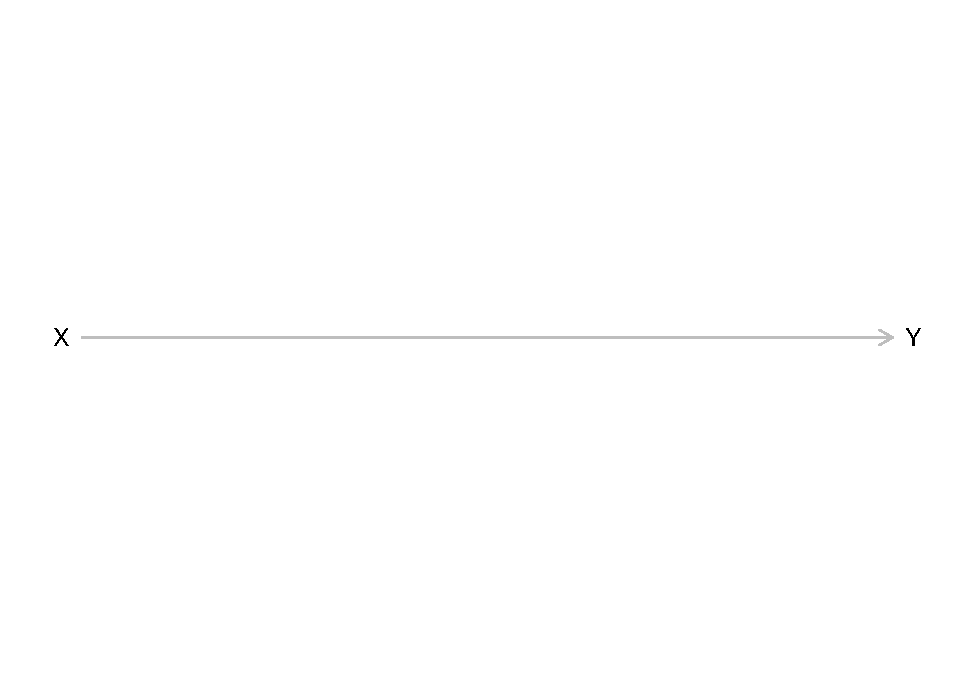
\includegraphics{_main_files/figure-latex/dag_directed-1.pdf}

What are the assumptions about the data generating process we have
encoded here? We have one dependent variable \(X\) that we assume to have
a direct effect on the independent variable \(Y\). We know that our
assumption was that \(X\) has an effect on \(Y\) and not the other way
around, because the arrow is \emph{directed} from \(X\) to \(Y\).

We call the sequence of one or many arrows that do not pass a single
variable more than once a \emph{path}. When trying to estimate an effect of
interest we are foremost interested in the paths going from our
independent variable of interest to the dependent variable. In the first
example we only have the one path \(X \rightarrow Y\), but in most ``real''
DAGs we will have multiple paths between \(X\) and \(Y\).

Consider this DAG, where we introduce a second variable \(A\):

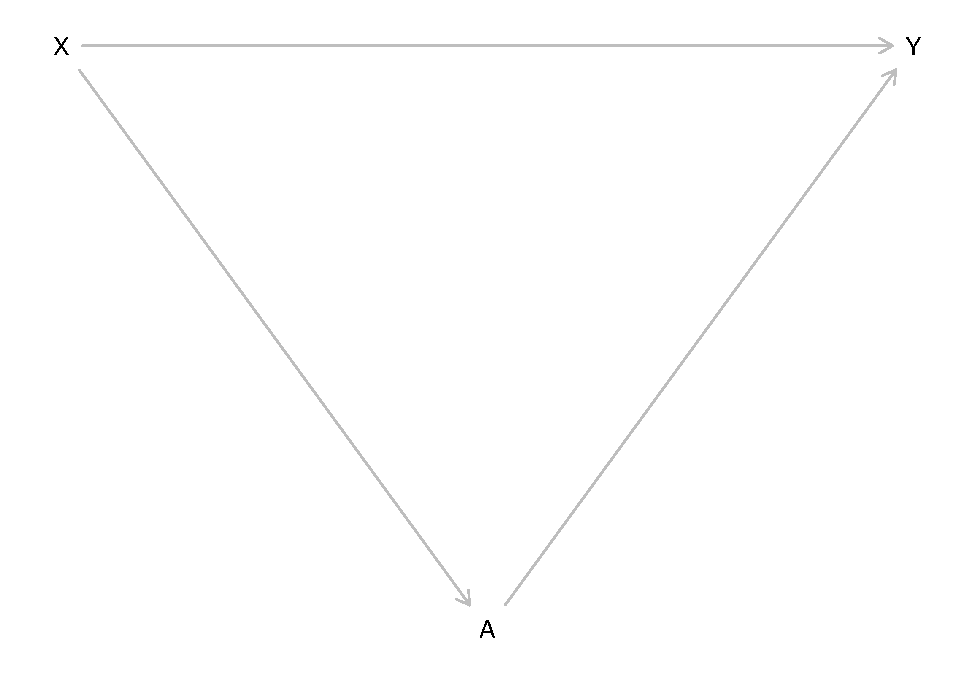
\includegraphics{_main_files/figure-latex/dag_paths-1.pdf}

Here there are two paths from \(X\) to \(Y\), \(X \rightarrow Y\) and
\(X \rightarrow A \rightarrow Y\). Our assumption here was that \(X\)
directly influences \(Y\), but that \(X\) also directly influences \(A\) which
in turn directly influences \(Y\). The latter is an indirect effect from
\(X\) on \(Y\) through \(A\).

DAGs are also \emph{acyclical}, meaning that there can not be any cyclical
relationships between variables. A cyclical relationship would be
present if we start from one variable and follow a path that leads us
back to this variable.

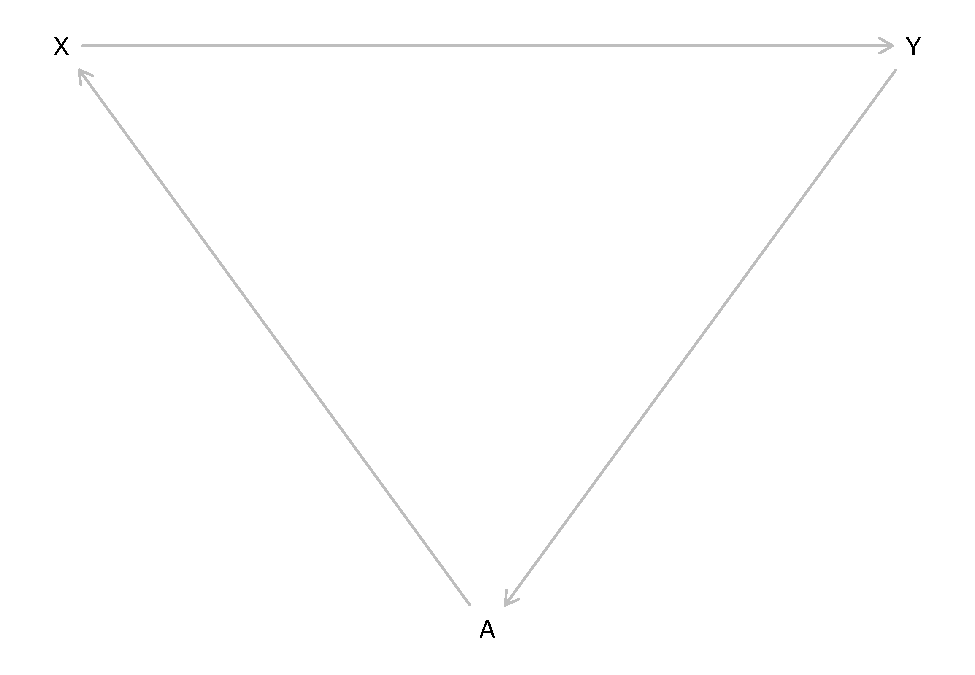
\includegraphics{_main_files/figure-latex/dag_acyclical-1.pdf}

In this example there is a path
\(X \rightarrow Y \rightarrow A \rightarrow X\) that leads us from \(X\)
back to \(X\). This is not allowed in a DAG.

Now that we know the basics, what do we actually do with a DAG? A DAG is
a way to graphically formalise our assumptions about the data generating
process. But it is about more than drawing nice formalisations, it is
also about figuring out which variables we have to include and which we
are not allowed to include to get an unbiased estimate of our effect of
interest. We do this by \emph{blocking} all paths from \(X\) to \(Y\) that do not
represent the relationship we want to estimate and at the same time
opening up all paths that do. For this to make sense, we need to know
the three patterns of relationships between a set of three variables and
how we can open or close paths with them.

\hypertarget{patterns-of-relationships}{%
\subsection{Patterns of relationships}\label{patterns-of-relationships}}

\hypertarget{chainspipe}{%
\subsubsection{Chains/Pipe}\label{chainspipe}}

Three variables can be connected in a \emph{chain} or \emph{pipe} like this:

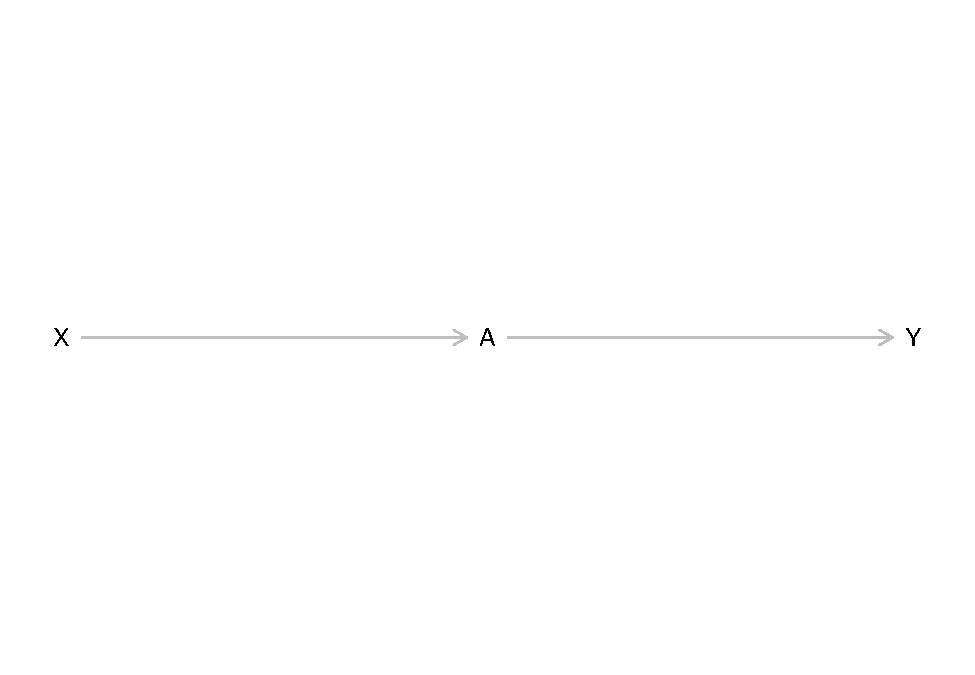
\includegraphics{_main_files/figure-latex/dag_pipe-1.pdf}

\(X\) has an effect on \(A\) which in turn affects the value of \(Y\). This
implies that \(X\) and \(Y\) are statistically correlated. When the value of
\(X\) changes, the value of \(Y\) also changes, ``transmitted'' by the
indirect effect \(X\) has on \(Y\) through \(A\). Remember we are still
interested in measuring the effect of \(X\) on \(Y\), so we also want to
measure this indirect effect.

The DAG tells us that there is a relationship between all three
variables. We therefore could be tempted to include \(A\) in our model as
well. But what would happen is that by including \(A\) we would \emph{block}
the path between \(X\) and \(Y\). We would not be able to measure the
association we are actually interested in. Including such a variable and
thereby blocking a path of interest is called \emph{overcontrol bias}.

In some cases overcontrolling can make the effect of interest
unmeasurable. We would then conclude from our analysis that \(X\) has no
effect on \(Y\) and that our hypotheses was wrong, while there actually
could be an effect that we made ``disappear'' by blocking its path.
Drawing a DAG based on our assumptions helps us to prevent this pitfall.

\hypertarget{mediation}{%
\paragraph{Mediation}\label{mediation}}

A special case of pipes is \emph{mediation}.

Consider this DAG:

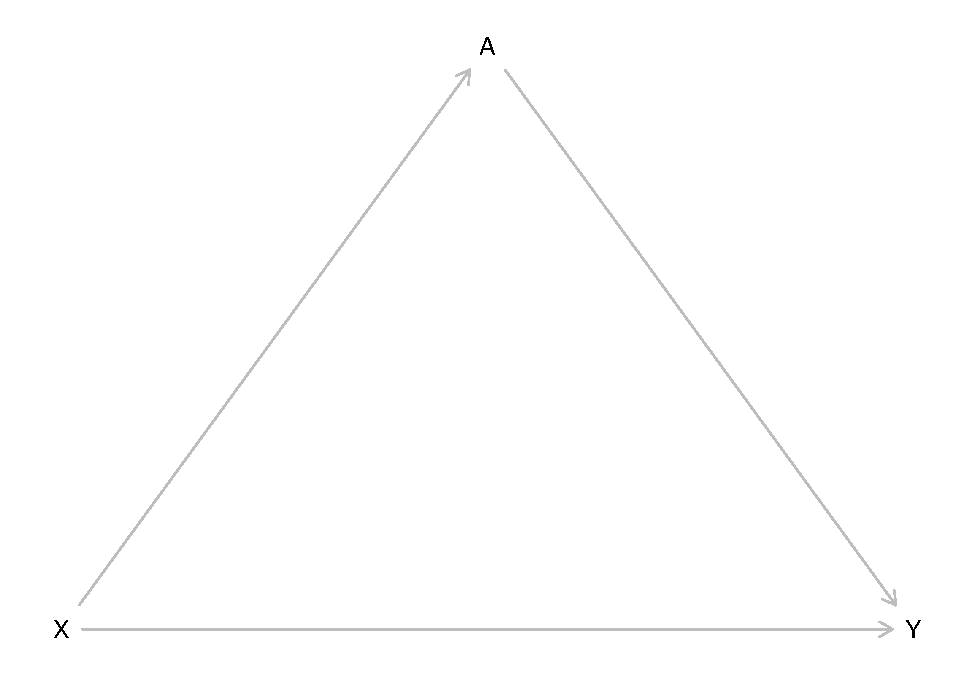
\includegraphics{_main_files/figure-latex/dag_mediation-1.pdf}

We see a direct effect through the path \(X \rightarrow Y\) as well as
indirect effect through \(X \rightarrow A \rightarrow Y\). Should we
include \(A\) in our model? This depends on what we want to measure.

If we are interested in the \emph{total effect} of \(X\) on \(Y\), we should not.
Both effects, the direct and the indirect paths, are of interest here,
so we keep both paths open by not controlling for \(A\).

Our interest could also lie exclusively in the \emph{direct effect}. Here we
would want to measure the effect of \(X\) stripped by all indirect
effects. In this case we want the path \(X \rightarrow Y\) to keep open,
but we would close the path \(X \rightarrow A \rightarrow Y\) by
controlling for \(A\).

We could also only be interested in the \emph{indirect effect}, the effect of
\(X\) on \(Y\) that goes through \(A\). We can not directly model this, but we
can compute the indirect effect as the difference between total and
direct effect.

\hypertarget{confounders}{%
\subsubsection{Confounders}\label{confounders}}

The second pattern we may see is the \emph{fork} or \emph{confounder}.

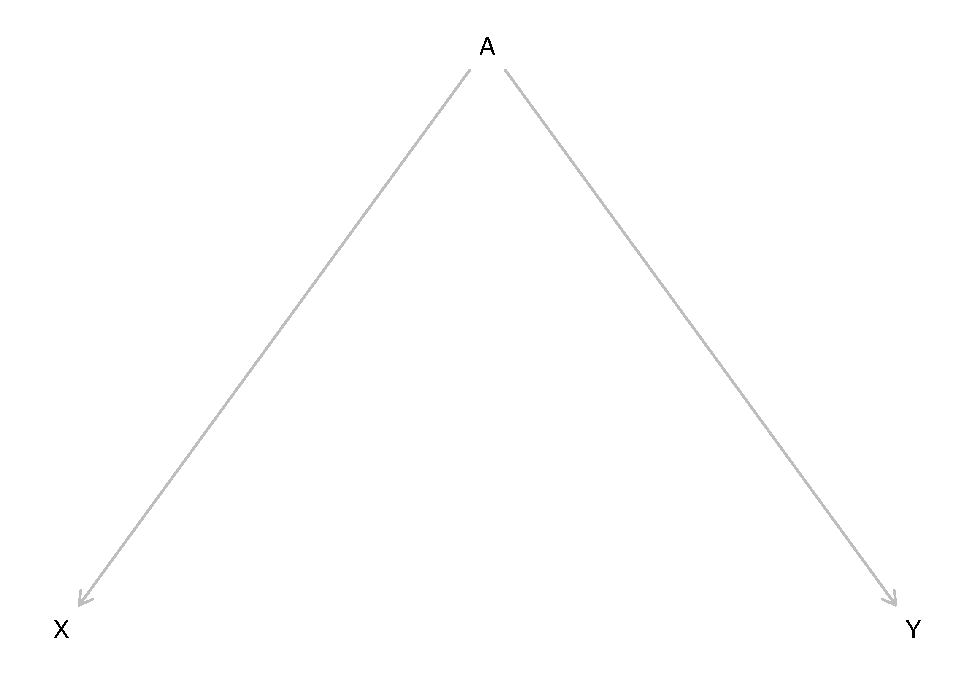
\includegraphics{_main_files/figure-latex/dag_confounder-1.pdf}

We see that there is no implied direct relationship between \(X\) and \(Y\)
but that both variables are influenced by \(A\). If we would measure the
relationship between \(X\) and \(Y\) we \emph{should} see no statistical
correlation. The problem is, that we \emph{would} see a correlation despite
this. Why is that? The values of \(X\) and \(Y\) both depend on the value of
\(A\). If we for example assume that both effects are positive the value
of \(X\) would rise with the value of \(A\) and the value of \(Y\) would rise
with the value of \(A\) also. The opposite would be true if both effects
were negative. Lower values for \(A\) would lead to lower values for \(X\)
and \(Y\). But even if the effects would be opposite, they would never
cancel each other out perfectly. \(X\) and \(Y\) vary together. If we just
include \(X\) and \(Y\) in our model this would show up as an effect from
\(X\) on \(Y\).

In DAG terms, there is an open path between \(X\) and \(Y\) although we did
not draw a direct path: \(X \leftarrow A \rightarrow Y\). This may seem
counterintuitive at first, as the arrows go in opposite directions, but
for paths in a DAG to exist, the direction of the arrows does not
matter. Every connection between variables is a path. So there is an
open path, in this case a so called \emph{backdoor path}, that leads to a
statistical association between \(X\) and \(Y\), but we can close it by
controlling for \(A\). If we do this, we would see no remaining
association between \(X\) and \(Y\) and thus get an unbiased estimate for
the effect of interest, i.e.~no effect.

If this still seems unintuitive consider the following example, which
you can also find in many statistical textbooks. Do storks bring babies?
We could tackle this analytically by taking a measure of babies born in
a region as our dependent variable and the number of storksightings in
the same region as our dependent variable. Let statistics come to the
rescue and help us discard the notion of the baby bringing stork once
and for all. But alas, our model will tell us that there is a positive
effect from storksightings on the number of newborns. Should we conclude
that everything we learned from our parents and teachers was one big lie
to hide away the magical truth about reproduction? Before we do that,
let us return to rationality. Maybe we have missed something important.
It turns out that there is a confounder we did not include in our model.
More rural areas have higher birthrates and also have a higher rate of
storksightings while both variables have lower values in more urban
regions. Our dependent and independent variables both vary by the value
of the confounder and thus it seems that there is a correlation where
there actually is none. If we now include a measure for the type of
region, let us say population density, this spurious association
disappears and we can return to normality. Storks do not bring babies
after all.

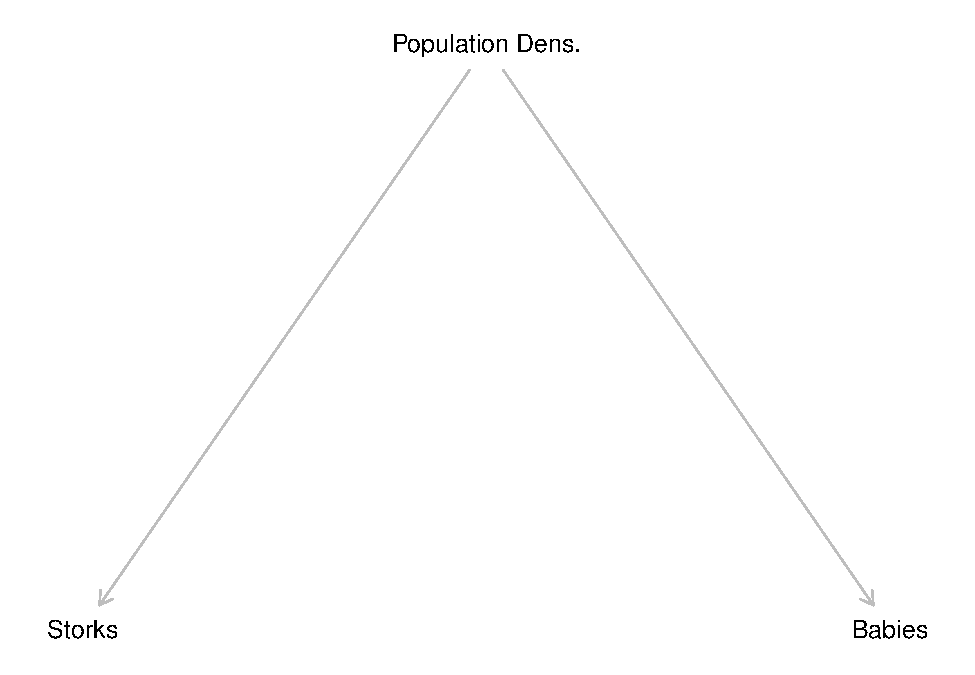
\includegraphics{_main_files/figure-latex/dag_storks-1.pdf}

\hypertarget{colliders}{%
\subsubsection{Colliders}\label{colliders}}

The last pattern we have to consider are \emph{colliders}. A collider is a
variable on a path that has two arrows pointing into it:

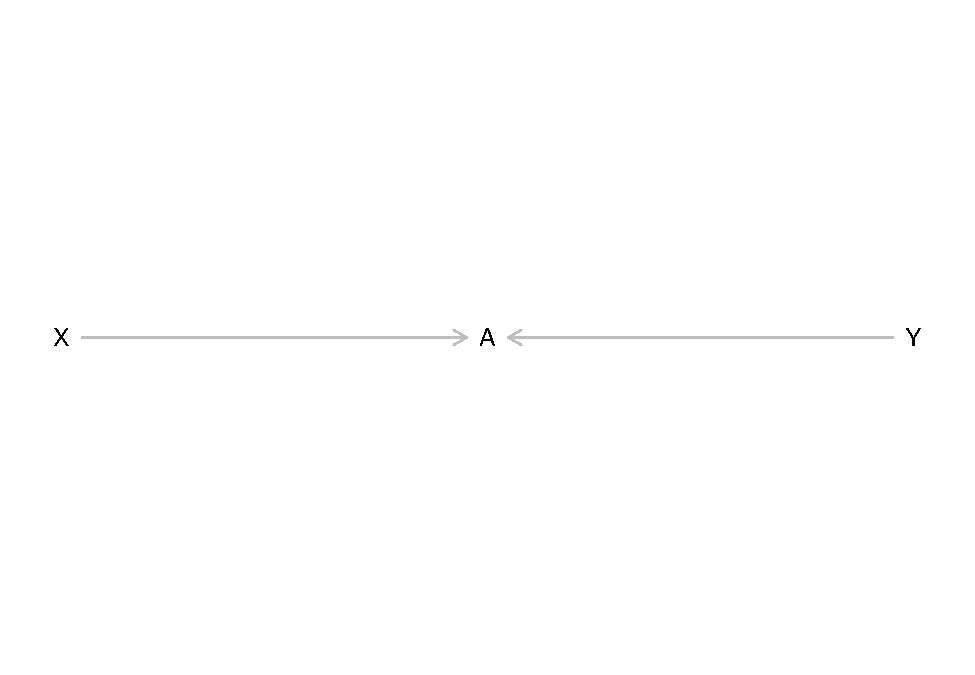
\includegraphics{_main_files/figure-latex/dag_mediation_1-1.pdf}

Here \(A\) is influenced by the value of \(X\) as well as \(Y\). Again, there
should be no effect of \(X\) on \(Y\) and in this case there is none if we
just include \(X\) and \(Y\) in our model. If we also include \(A\) we
introduce an association between \(X\) and \(Y\) even if there should be
none. This implies that we should not control for colliders because we
would open up a path that creates a spurious association between two
variables that are not related.

\hypertarget{adjustment-set}{%
\subsection{Adjustment set}\label{adjustment-set}}

Now we have all the building blocks for identifying which variables we
have to include in our model and which we are not allowed to include. If
we do not follow these rules we may statistically find relationships
where there are none or miss relationships that actually exist. We then
would draw the wrong conclusions for our hypotheses and research
question. We would produce bad science.

If we draw out our DAG and use its implications to identify the correct
\emph{adjustment set} \(Z\) of control variables, we do not fall into this
trap. We only control what we have to, and nothing that we should not.
We thus create the best model to get an unbiased estimate for our effect
of interest; but there is always a caveat and this is a big one. The
model is only correct if our DAG is also correct and we can never know
for certain if it is. We could make wrong assumptions, forget important
relationships, and make all matters of mistakes while building our DAG.
While DAGs are a great tool for identifying the adjustment set, the
technique alone can never replace careful thinking.

\hypertarget{nba-dag}{%
\section{NBA DAG}\label{nba-dag}}

We will now pick up where we left off in session 2 and return to the NBA
data. Equipped with our new tool we can now draw a DAG with the goal of
building a model to estimate the effect of points scored on the salary a
player receives. The assumption is, that the higher the point average,
the higher the salary. This makes intuitive sense as a high scoring
player is more valuable to the team and thus may receive a higher
monetary compensation.

Let us start building a DAG with the information we already have.

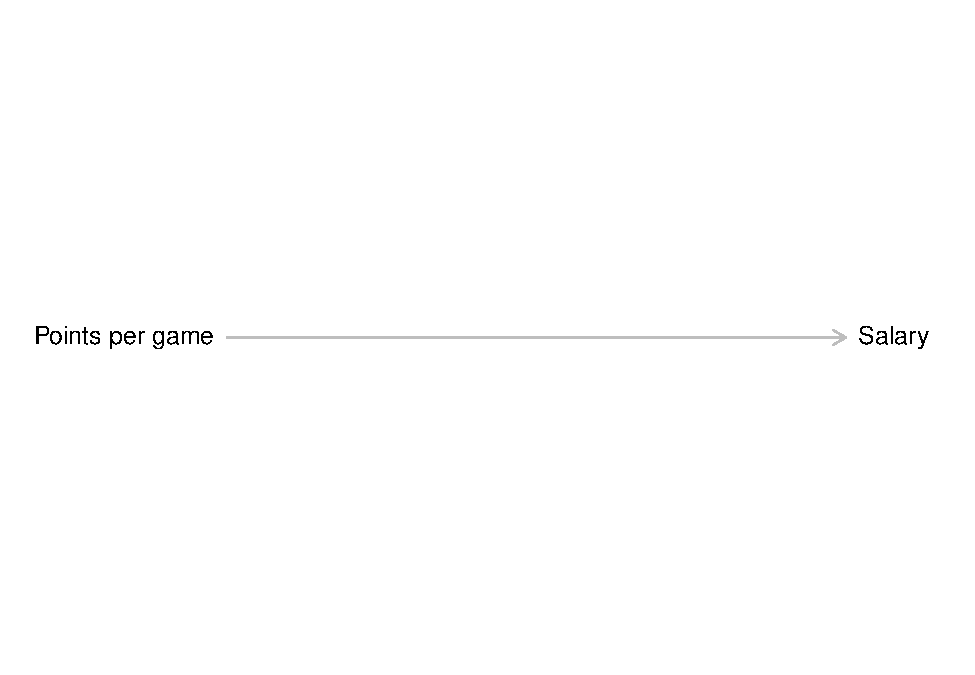
\includegraphics{_main_files/figure-latex/dag_1-1.pdf}

Now we have to think about other factors that could influence the
relationship between points and salary. One variable we already
identified as having an effect on both was the position a player
occupies. The position influences how many points per game a player can
score and we also already saw that centers make more money compared to
point guards. Right now we have no reason to believe that other
positions do not also have an effect on the received salary. Following
this reasoning, position is a confounder for points and salary.

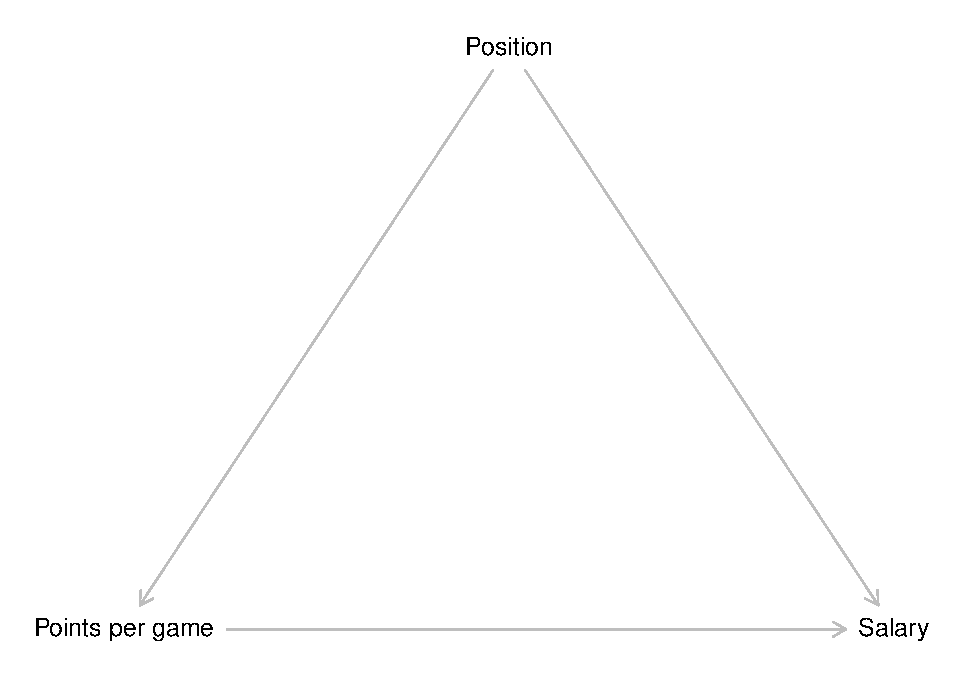
\includegraphics{_main_files/figure-latex/dag_2-1.pdf}

It is also reasonable that body height influences which position a
player can occupy. Centers have to be big while smaller players tend to
play on other positions. At the same time, height is an advantage if you
want to score in a basketball game. Thus height is a confounder for
points and position.

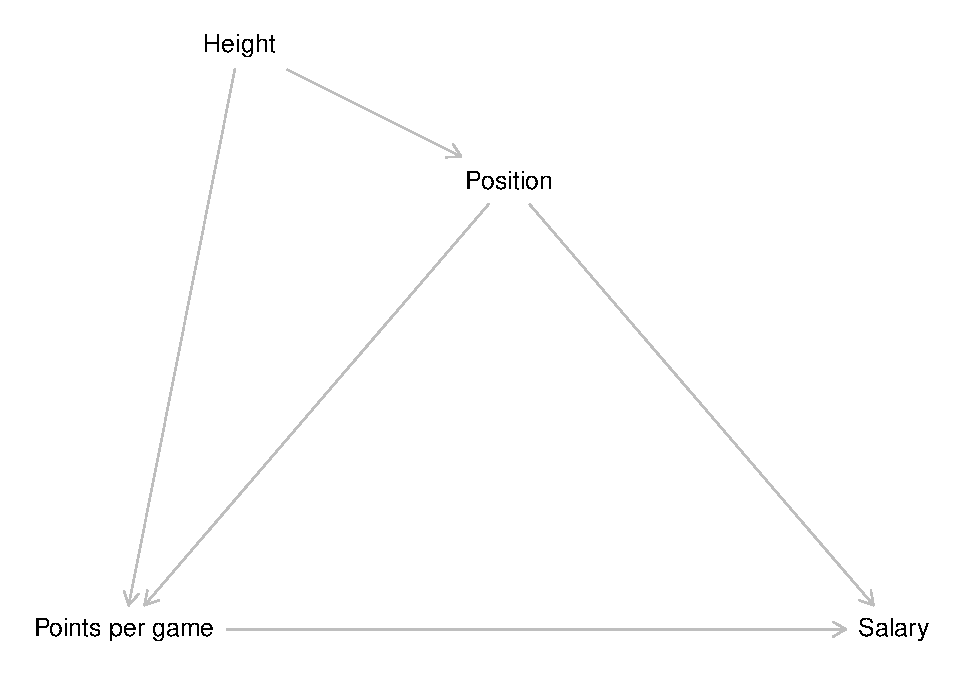
\includegraphics{_main_files/figure-latex/dag_3-1.pdf}

Another factor that will have an effect on the salary is the team a
player plays for. More successful teams will be able to pay higher
salaries. The season an observation was recorded in should also
influence the paid salary as we can expect a general inflation of
salaries over time.

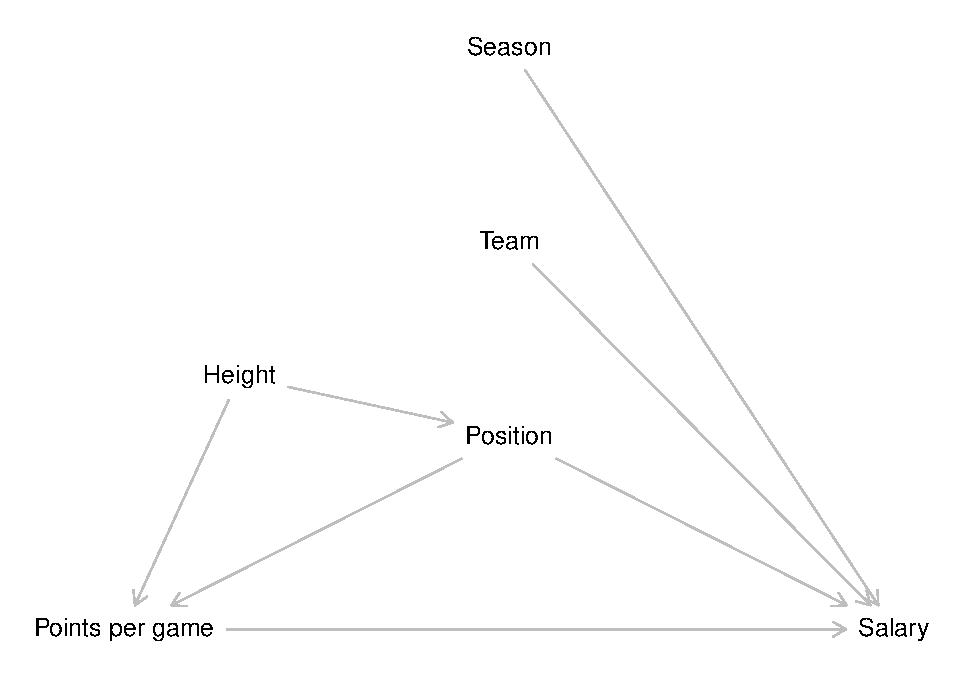
\includegraphics{_main_files/figure-latex/dag_final_0-1.pdf}

This is our final DAG. Does it correctly depict the underlying data
generating process? We do not know for sure, but the DAG correctly
reflects our assumptions at this point. Those may be wrong. Maybe the
data generating process actually works slightly or even completely
different; but to the best of our current knowledge, this is how the
scored points affect the salary a player receives.

We can now inspect what implications the DAG has for our model. To do
this, let us list the paths from our independent to the dependent
variable.

\[A: Points \rightarrow Salary\]
\[B: Points \leftarrow Position \rightarrow Salary\]

\[C: Points \leftarrow Height \rightarrow Position \rightarrow Salary\]
Path A is a direct path from our independent variable to our dependent
variable. We will have to include scored points and salary into our
model, but that is a given.

Paths B \& C are both backdoor paths - these are easily spotable by an
arrow pointing into the independent variable - that we have to address
somehow. Let us consider B first. Position is a confounder for points
and salary. Above we already learned how to deal with this, we control
for it. This removes the spurious part of the association between points
and salary introduced by the confounder. Path C also includes a
confounder, namely the body height of a player. Do we also control for
this variable to close path C? No, we do not. If we further examine path
C we will see that it also includes position as a pipe. When we control
for a variable in a pipe, the path gets closed. As we have to include
position to close path B, path C is also already closed.

The two remaining variables, team and season, have direct effects on the
salary but do not lie on a path from points to salary. This implies,
that we do \textbf{not} have to control for them if our goal is estimating
the effect of points on salary.

Above we briefly talked about the two possible goals of modelling. Here
and over the next sessions our goal is estimating an effect of interest
without bias. We used the DAG to identify an adjustment set of variables
we have to control for to reach this goal. If our goal was predicting
the salary as accurately as possible we would made other conclusions.
The team a player is employed by and the season where an observation was
measured are both relevant predictors for the received salary. For
prediction we would have included both variables because this should
increase the accuracy of the prediction. We will return to this in more
detail in \protect\hyperlink{pm-t}{session 11}.

\hypertarget{resources}{%
\section{Resources}\label{resources}}

\hypertarget{dagitty.net}{%
\subsection{dagitty.net}\label{dagitty.net}}

While the underlying rules of DAGs are relatively straightforward,
identifying the adjustment set can get harder the more complex a DAG
gets. Consider this for instance:

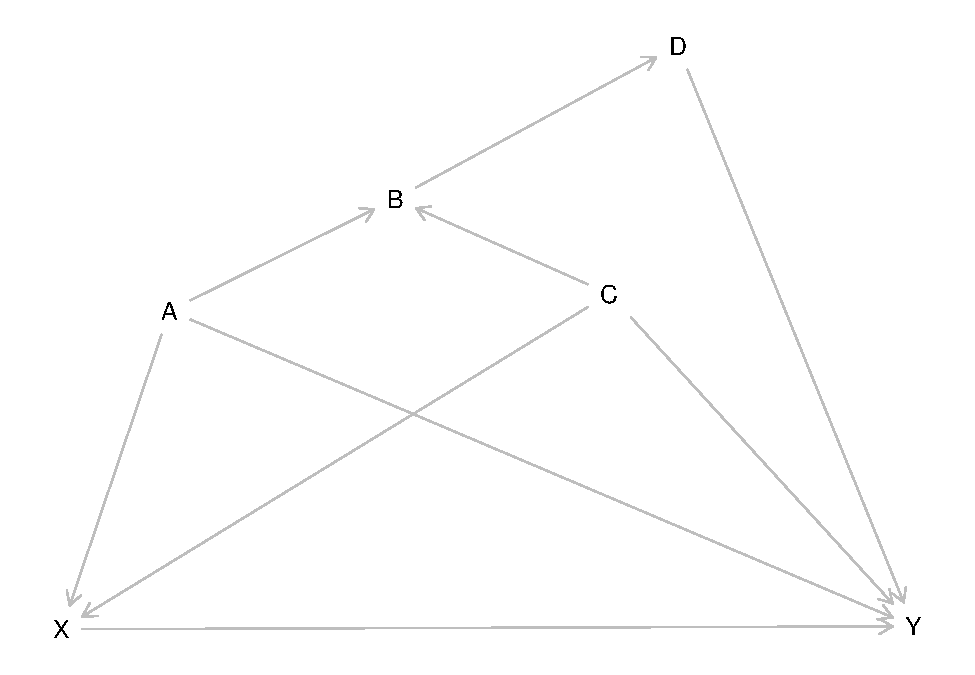
\includegraphics{_main_files/figure-latex/dag_final_1-1.pdf}

What variables do we have to include in our adjustment set to get
unbiased measure for the effect from \(X\) on \(Y\)? We would suggest you
take out pen and paper and try to figure it out. You can approach this
as above. List all paths from \(X\) to \(Y\) that do not include a variable
twice and try to find the adjustment set that closes all paths besides
the one(s) needed to measure the effect from \(X\) on \(Y\). Spoiler: In
this case the only path we want to keep open is the direct effect
\(X \rightarrow Y\).

While this is doable, you may be unsure if you found the correct set.
Luckily there is a convenient way to find out. \url{https://dagitty.net/}
provides a browser tool where you can draw DAGs - as well as export them
for your papers - and check for the correct adjustment set. After
launching the tool you should click on ``Model'' and then ``New model''. Now
you can start drawing. New variables are added by clicking on the canvas
and naming them, arrows are added by first clicking on the variable
where the arrow should start and then on the variable where it should
end. For everything to work you should also declare the independent
variable of interest the ``Exposure'' and the dependent variable the
``Outcome''. Both can be set on the left under ``Variable''. When the DAG is
drawn correctly, the top right panel ``Causal effect identification''
should show which variables need to be part of the adjustment set to
estimate the effect of interest.

Note that ``Causal effect identification'' is set to display the
adjustment set for the total effect. This also is what we are interested
in here. If we are interested in mediation, we can also set the panel to
display the set for the direct effect.

\hypertarget{how-to-use-dagitty}{%
\subsection{How to use dagitty()}\label{how-to-use-dagitty}}

We can also draw DAGs directly in R, using the \texttt{dagitty} package. To
start drawing a DAG we write \texttt{dagitty(\textquotesingle{}dag\ \{\})}. The actual definition
of the DAG takes place between the squirly brackets. First we list all
variables in the model by writing their names between quotation marks.
For each variable we can optionally add additional options between
square brackets following the name. In the example below we define one
variable as \texttt{exposure} and one as \texttt{outcome}, just like we would do on
dagitty.net. We also give values for the relative positions. If we skip
those, \texttt{dagitty()} will decide on the positions itself which may or may
not look nice and tidy. After all variables are defined we write out the
paths that should be present connecting the variable names with \texttt{\textless{}-} or
\texttt{-\textgreater{}}, depending on the direction an arrow should point. We can than use
\texttt{plot()} to see the DAG.

\begin{Shaded}
\begin{Highlighting}[]
\CommentTok{\# Load the dagitty package}
\FunctionTok{library}\NormalTok{(dagitty)}

\CommentTok{\# Define a DAG}
\NormalTok{dag }\OtherTok{\textless{}{-}} \FunctionTok{dagitty}\NormalTok{(}\StringTok{\textquotesingle{}dag \{}
\StringTok{  "Exposure" [exposure, pos="{-}1,0"]}
\StringTok{  "Outcome" [outcome, pos="1,0"]}
\StringTok{  "Confounding Variable" [pos="0,{-}1"] }
\StringTok{  "Mediator" [pos="0,1"]}
\StringTok{  "Exposure" {-}\textgreater{} "Outcome"}
\StringTok{  "Exposure" {-}\textgreater{} "Mediator" {-}\textgreater{} "Outcome"}
\StringTok{  "Exposure" \textless{}{-} "Confounding Variable" {-}\textgreater{} "Outcome"}
\StringTok{\}\textquotesingle{}}\NormalTok{ )}

\CommentTok{\# Plot the DAG}
\FunctionTok{plot}\NormalTok{(dag)}
\end{Highlighting}
\end{Shaded}

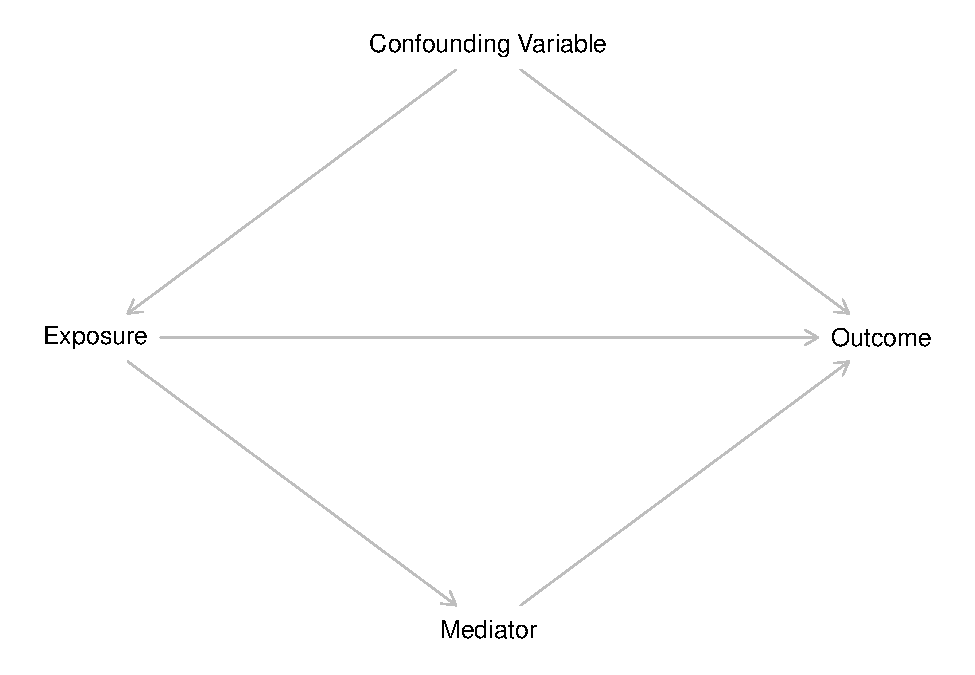
\includegraphics{_main_files/figure-latex/dagitty_example-1.pdf}

We can also use the function \texttt{adjustmentSets()} to derive our adjustment
set. The argument \texttt{effect\ =} lets us control if we want to see the
adjustment set for the \texttt{"total"} or \texttt{"direct"} effect.

\begin{Shaded}
\begin{Highlighting}[]
\CommentTok{\# Identify the minimal adjustment set for estimating the total effect of Exposure on Outcome}
\FunctionTok{adjustmentSets}\NormalTok{(dag, }\AttributeTok{effect =} \StringTok{"total"}\NormalTok{)}
\end{Highlighting}
\end{Shaded}

\begin{verbatim}
## { Confounding Variable }
\end{verbatim}

\begin{Shaded}
\begin{Highlighting}[]
\CommentTok{\# Identify the minimal adjustment set for estimating the direct effect of Exposure on Outcome}
\FunctionTok{adjustmentSets}\NormalTok{(dag, }\AttributeTok{effect =} \StringTok{"direct"}\NormalTok{)}
\end{Highlighting}
\end{Shaded}

\begin{verbatim}
## { Confounding Variable, Mediator }
\end{verbatim}

\hypertarget{more-on-dags}{%
\subsection{More on DAGs}\label{more-on-dags}}

If you are interested in diving deeper into DAGs, we can recommend this
resources, which were also used for writing this session.

Richard McElreath provides a great introduction into the topic with many
clear examples. While the book chapter on DAGs may require some
knowledge of advanced statistical topics, the corresponding lecture on
YouTube is more approachable:

McElreath, Richard (2020). Statistical Rethinking: A Bayesian Course
with Examples in R and STAN. Second Edition. Boca Raton \& Oxon: CRC
Press. Chapter 5: The Many Variables \& The Spurious Waffles, 123-160.

Corresponding YouTube lecture:
\url{https://www.youtube.com/watch?v=mBEA7PKDmiY}

\hfill\break

Felix Elwert wrote a concise paper on DAGs with a perspective that is
more focused on causality than we have presented here:

Elwert, Felix (2013). Graphical Causal Models. In S. L. Morgan (Hrsg.),
Handbook of Causal Analysis for Social Research, 245--273. Dordrecht
{[}u.a.{]}: Springer.

\hfill\break

If you really want to get into it, the work of Judea Pearl was central
for establishing DAGs. An approachable starting point would be the ``Book
of Why'':

Pearl, Judea \& Dana Mackenzie (2018). The book of why : the new science
of cause and effect. New York: Basic Books.

\hypertarget{lin-t-1}{%
\chapter{Linear Regression - Theory I: Simple Linear Regression}\label{lin-t-1}}

The next three sessions will comprise an introduction for linear regressions.
We will look at the theoretical underpinnings, the interpretation of results
and the underlying assumptions of these models. For this introduction we will
keep the NBA data aside and use some simulated data that plays nice with us.
We will return to the NBA data in session 8 applying everything we
learned to assess the effect of scored points on salary.

\hypertarget{objectives-2}{%
\section{Objectives}\label{objectives-2}}

\begin{itemize}
\tightlist
\item
  Understand simple linear regression
\item
  Understand the regression formula
\item
  Interpret the results
\end{itemize}

\hypertarget{what-is-linear-regression}{%
\section{What is Linear Regression}\label{what-is-linear-regression}}

As we eluded to last session, there are two main approaches to using
statistical modelling in the social sciences.
The more classical approach is to use modelling for estimating the effect that
one or several independent variables have on one dependent variable. Maybe we
are interested in knowing if a higher income has an effect on life satisfaction
and if yes, what the direction and magnitude of this effect is. Does more money
actually make you happier?

The other and more recent approach is to use modelling for making predictions
with high accuracy. Based on the relationships between many independent
variables and one dependent variable. We try to predict the latter for actual
or hypothetical cases based on their values for the independent variables.
This approach lies at the heart of \emph{machine learning} and drives many of the
technologies we use on a daily basis from E-Mail spam filters to ChatGPT.
Returning to the example above, we are not interested in measuring the \emph{effect}
of money on life satisfaction, but in \emph{predicting} the value for life satisfaction
based on money and a host of other variables as accurately as possible.

Linear regression is one of the many available modelling techniques and it can
serve both approaches. Over the next sessions we will focus on using
linear regression for estimating an effect of interest but we will return to
prediction in \protect\hyperlink{pm-t}{session 10}.

How do we know if we should choose linear regression for a specific task?
This is not easy to answer as there are many alternatives and even variations of
linear regression which may be better suited for a specific empirical problem.
As this is an introduction to modelling and time is of the essence we opted to
mainly focus on an in-depth introduction to linear regression.
This technique is suited for many problems and
is comparably easy to understand and use. Also, after learning the ins and outs
of linear regression, we are in a good position to build upon that knowledge and
learn all of those more complex and specific models that we will encounter in
textbooks and scientific papers.

With the pool of options trimmed down to one, the central question remains unanswered.
Should I use linear regression for my task? As we have no alternatives to chose
from, we can change the question to: Can I use linear regression for my task?
The answer mainly depends on what type of dependent variable we want to use.
If it is metric, we can use linear regression.
In our cases the dependent variable is metric, as you will find out below.
If we had other types of dependent variables we would have to use different
models.
For example a common choice for binary or categorical dependent variables is
logistic regression, which we will introduce at a \protect\hyperlink{log-est}{later point in the course}.

\hypertarget{examplary-research-question-data}{%
\section{Examplary research question \& data}\label{examplary-research-question-data}}

For this introduction, let us imagine that we are interested in a research
question that asks: \emph{What makes a good grade in a seminar paper?} In particular we
are interested in the effect that the hours a student invests in working on it
has on the grade. Based on some theoretical considerations, and maybe some
idealistic views, we derive our main hypotheses that putting in more hours will
result in a better grade.

Now we also - hypothetically - held a small survey and asked 200 imaginary
students some questions on how they approached writing a seminar paper. In
particular we asked them how much time they spent working on the paper, if they
have attended (almost) all seminar sessions, how closely they worked with their
lecturers in preparing the paper and what the mean grade for previous papers
was. As these imaginary students have already turned in their papers, we also
know the grades they achieved.

Please note, that this is data on \textbf{imaginary} students, meaning we have
simulated the data making some assumptions on how to achieve a good (or bad)
grade in a paper. The assumptions we made do not necessarily reflect the way
\emph{you} write a good paper, while still being based in our experience on what it
takes to achieve a good grade. But remember, no real students were harmed in
making up this data.

Let us have a first look on the data:

\begin{verbatim}
## -- Data Summary ------------------------
##                            Values
## Name                       grades
## Number of rows             200   
## Number of columns          7     
## _______________________          
## Column type frequency:           
##   factor                   1     
##   logical                  1     
##   numeric                  5     
## ________________________         
## Group variables            None  
## 
## -- Variable type: factor -------------------------------------------------------
##   skim_variable n_missing complete_rate ordered n_unique
## 1 contact               0             1 FALSE          3
##   top_counts               
## 1 No : 80, In : 70, E-M: 50
## 
## -- Variable type: logical ------------------------------------------------------
##   skim_variable n_missing complete_rate  mean count            
## 1 attendance            0             1 0.765 TRU: 153, FAL: 47
## 
## -- Variable type: numeric ------------------------------------------------------
##   skim_variable            n_missing complete_rate      mean    sd     p0    p25
## 1 grade                            0             1  2.97e+ 0 1.08    1     2.1  
## 2 hours                            0             1  4.03e+ 1 6.29   23    36    
## 3 previous_grades                  0             1  2.94e+ 0 0.965   1     2.3  
## 4 previous_grades_centered         0             1 -7.21e-17 0.965  -1.94 -0.635
## 5 hours_centered                   0             1  1.70e-15 6.29  -17.3  -4.33 
##       p50   p75  p100 hist 
## 1  3       3.73  5    ▅▆▇▆▅
## 2 41      45    57    ▁▅▇▅▁
## 3  2.95    3.62  5    ▅▇▇▆▂
## 4  0.0150  0.69  2.06 ▅▇▇▆▂
## 5  0.670   4.67 16.7  ▁▅▇▅▁
\end{verbatim}

Right now, the observations are ordered by the grade of the seminar paper which
run from \(1.0\) to \(5.0\) in increments of \(0.1\). While this is somewhat
unrealistic - the German grading system actually only uses the increments \(.0\),
\(.3\) and \(.7\) - simulating the data in this way will make the demonstrations on
linear regression easier and more straightforward. The variable
\texttt{previous\_grades} is set up in the same way and represents the mean of the
grades the student received up to this point. \texttt{hours} represents the time a
student spent on writing the paper, ranging from \(23 - 57\) hours, with a mean of
about \(40\). Besides these metric variables, the data set also contains two
categorical measures. \texttt{attendance} is a \emph{binary} or \emph{dummy variable}, meaning it can only
have the values \(1\) or \(0\) or \texttt{TRUE} and \texttt{FALSE} in this case, as it is saved as
a logical variable. \texttt{TRUE} represents that a student attended almost all seminar
sessions before writing the paper - which about \(77%
\) did -, \texttt{FALSE} states that
they did not.
\texttt{contact} is a factor variable with three categories and shows the answers to
the imaginary question on how much contact the student had to the lecturer
before starting the writing process. Besides \texttt{No\ contact} the students could
have had \texttt{E-Mail} contact to state their research question and get some short
written feedback or meet the lecturer \texttt{In\ Person} to achieve a deeper discussion
of the question and the laid out plan for writing the paper.
The two additional variables are versions of \texttt{previous\_grades} and \texttt{hours} that
are centered on their respective means. They will come into play at a later
point in this session.

Let's have a look at some observations.

\begin{verbatim}
## # A tibble: 10 x 7
##    grade hours previous_grades attendance contact   previous_grades_centered
##    <dbl> <int>           <dbl> <lgl>      <fct>                        <dbl>
##  1     1    50             1.4 TRUE       E-Mail                      -1.54 
##  2     1    46             1   TRUE       E-Mail                      -1.94 
##  3     1    42             1   TRUE       In Person                   -1.94 
##  4     1    49             1   FALSE      In Person                   -1.94 
##  5     1    42             1.2 TRUE       In Person                   -1.74 
##  6     1    46             1.8 TRUE       In Person                   -1.14 
##  7     1    44             1.4 FALSE      In Person                   -1.54 
##  8     1    45             2   TRUE       In Person                   -0.935
##  9     1    48             1   TRUE       In Person                   -1.94 
## 10     1    45             2   TRUE       In Person                   -0.935
## # i 1 more variable: hours_centered <dbl>
\end{verbatim}

From this first 10 rows, we can see that the students with the best grades spent
more than 40 hours on writing, have already achieved good grades in their papers
up to this point and at least had some contact to the lecturers. Most also
regularly attended the seminar but two did not and still achieved a \(1.0\) in
their grade.

So what makes a bad grade?

\begin{verbatim}
## # A tibble: 10 x 7
##    grade hours previous_grades attendance contact    previous_grades_centered
##    <dbl> <int>           <dbl> <lgl>      <fct>                         <dbl>
##  1   4.8    37             4.2 TRUE       No contact                    1.27 
##  2   4.8    38             4.3 TRUE       E-Mail                        1.36 
##  3   4.8    35             4.4 TRUE       E-Mail                        1.47 
##  4   4.9    40             4.2 TRUE       E-Mail                        1.27 
##  5   5      35             3.9 FALSE      No contact                    0.965
##  6   5      41             4.9 TRUE       No contact                    1.97 
##  7   5      24             4.7 TRUE       E-Mail                        1.76 
##  8   5      33             5   TRUE       E-Mail                        2.06 
##  9   5      29             4.1 FALSE      E-Mail                        1.16 
## 10   5      50             4.6 FALSE      E-Mail                        1.66 
## # i 1 more variable: hours_centered <dbl>
\end{verbatim}

Here the picture seems less clear. While most students did not put in as many
hours, some did and still failed to pass. Half of the students that received a
\(5.0\) regularly attended and most at least had E-Mail contact before writing
their paper. What seems to be more consistent though is that the mean of the
previous grades is rather low.

So what do we know now? Does a good or bad track record in grades predict all
future grades? This seems not only unrealistic but is also a kind of sad take home
message. To get a better understanding on which of the potential influential
variables has an effect on the final grade and what the magnitude and direction
of these effects is, we now turn to linear regression.

\hypertarget{simple-linear-regression}{%
\section{Simple Linear Regression}\label{simple-linear-regression}}

In a \emph{simple linear regression}, the model is used to describe the relationship
between \emph{one} dependent and \emph{one} independent or explanatory variable. The
question this model can answer for us is: By how much does the dependent
variable increase or decrease, when the explanatory variable increases by \(1\)?

Returning to our exemplary research question on what makes a good grade in a
seminar paper, an intuitive hypotheses would be that the grade gets better the
more hours a student invests in writing the paper. In this case we assume a
linear relationship between the independent variable \texttt{hours} and the dependent
variable \texttt{grade}. As German grades are better the lower their value, we thus
would assume a negative effect from \texttt{hours} on \texttt{grade}.

Before turning to the formalities and practical application of a simple linear
regression model, let us first have a look on this relationship by plotting the
variables against each other.

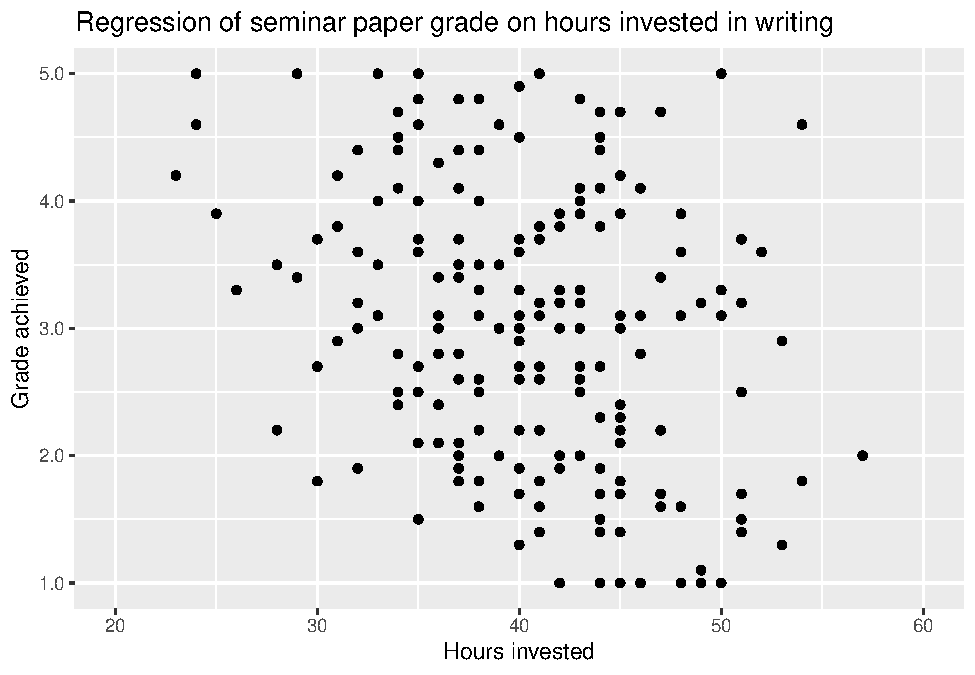
\includegraphics{_main_files/figure-latex/plot_grade_hours-1.pdf}

When we are talking about dependent and independent variables, there is the
convention to plot the former on the y-axis and the latter on the x-axis. So the
\emph{y-variable} is to be explained and the \emph{x-variable} is used to explain it.
This convention will also be used in all formulas in this seminar.

Looking at the plot we first see a cloud of dots, representing all combinations
of \texttt{hours} and \texttt{grade} in all our \(200\) observations. It may be hard to pick out
any pattern, but looking closely we can observe that overall the dots seem to
follow a downward slope from the upper left - indicating few hours worked and a
worse grade - towards the lower right - indicating more invested hours and a
better grade. This would be the relationship stated in our hypotheses. The more
hours a student works on a seminar paper the better the final grade will be.

We can try to describe this pattern by adding a line from the upper left to the
lower right.

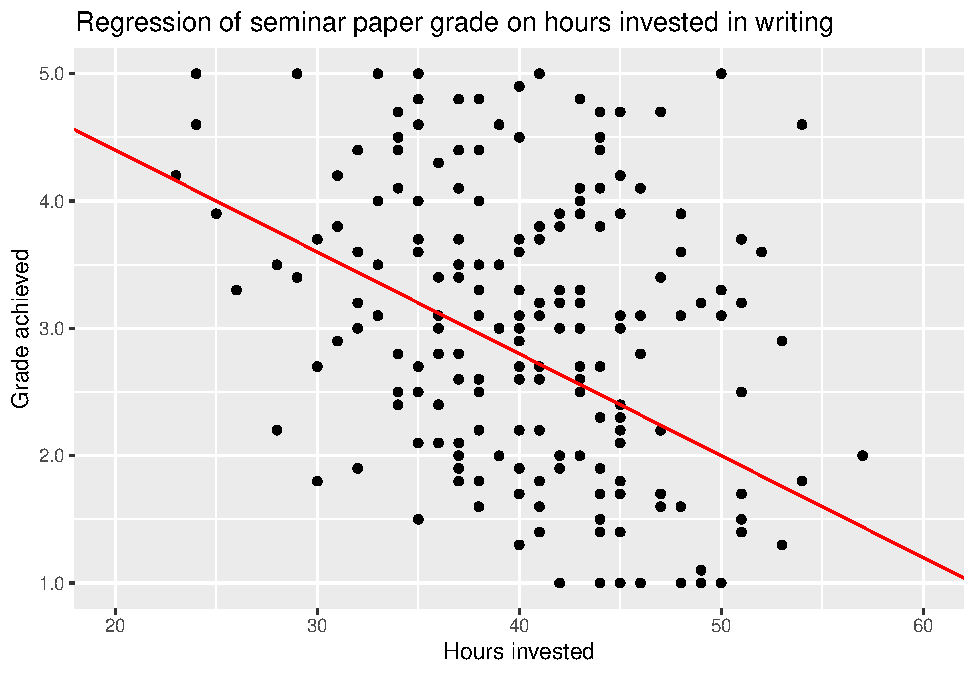
\includegraphics{_main_files/figure-latex/plot_grade_hours_wild_guess-1.pdf}

This describes the relationship between the two variables as linear. Each hour
invested decreases the grade by a certain amount, for this proposed line by
exactly \(0.08\) points. Remember that decreasing the value of the grade actually
means getting a better grade.

But is this the only possible line or even the \emph{correct} one? Most certainly not,
as the values used to draw the line were only a wild guess. We
could imagine several other lines that also look more or less reasonable - as
well as some that look unreasonable - and add them to the plot.

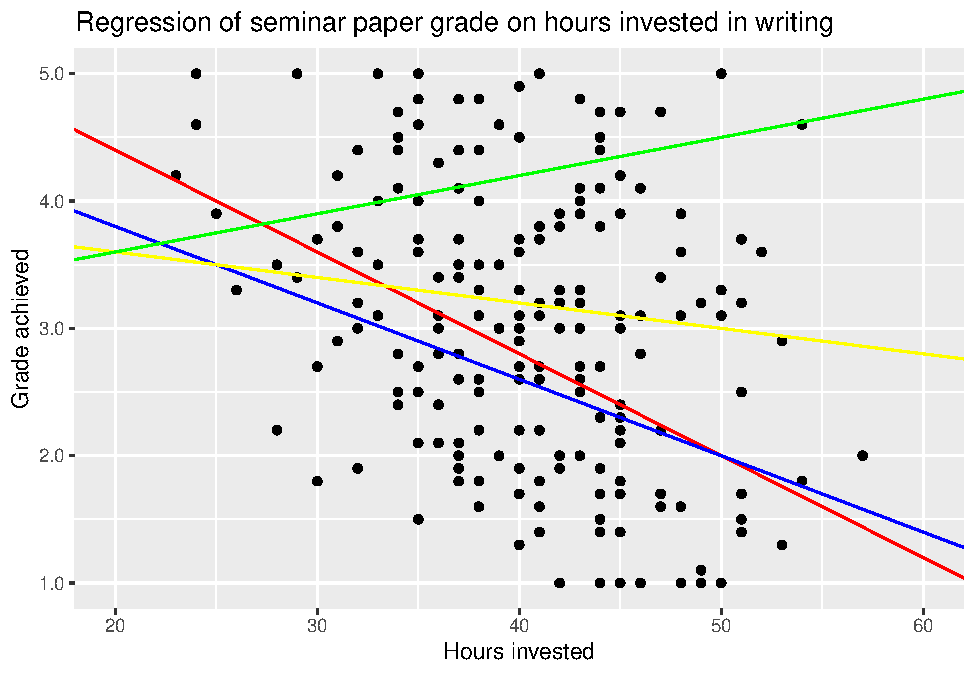
\includegraphics{_main_files/figure-latex/plot_grade_hours_wild_guesses-1.pdf}

While we have some intuition that the green line completely misses the mark, we
can't really decide between the others just by looking at the plot. The
data points are way to dispersed to see the relationship clearly.

The goal of using a simple linear regression model is to identify the \emph{one} line
that describes the relationship the best. Here \emph{best} means, with as little
error as possible.

\hypertarget{regression-formula}{%
\subsection{Regression Formula}\label{regression-formula}}

To understand how these lines in the above plot were conceived and how to find
the line with the best \emph{fit}, i.e.~the lowest error, we have to understand the
formula for linear regression. While formulas may always be kind of daunting,
we are in luck as this particular one is actually quite easy to understand,
especially when paired with a graphical representation.

\[y = \beta_0 + \beta_1*x_1 + \epsilon\]

Let us first look at the parts we already know. \(y\) is the dependent variable,
in our case the grade achieved. So one thing is for sure, the whole right part
of the equation has to be used to calculate the value of \(y\) from the data, i.e.
from the dependent variable \(x\). Here we have three terms. Let us skip the first one
for now and focus on the second one \(\beta_1*x_1\).

\(x_1\) is the dependent variable, in our case \texttt{hours}. \(\beta_1\) is the
\emph{regression coefficient} for \(x_1\). This value gives us the \emph{slope} of the
regression line. Based on this, we can start rewriting the general formula and
tailor it to our specific use case.

\[y_{grade} = \beta_0 + \beta_{hours}*x_{hours} + \epsilon\]

Let us return to the first wild guess we made above.

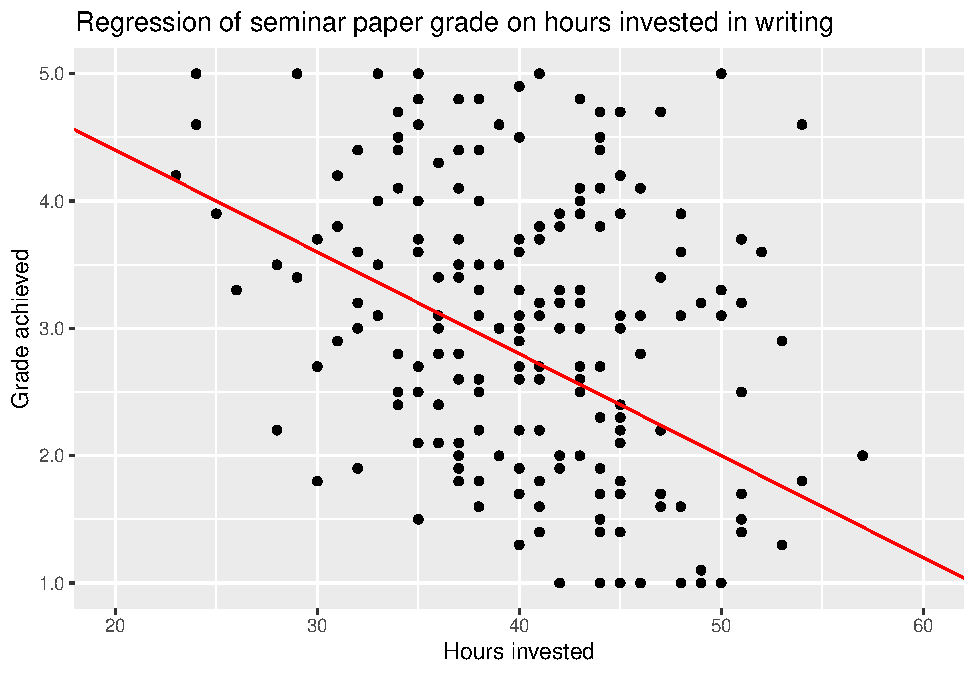
\includegraphics{_main_files/figure-latex/plot_grade_hours_wild_guess_expl_slope-1.pdf}

Here we guessed that an increase in invested time of one hour decreases the
value of \texttt{grade} by \(0.08\). This is the slope of the red line and thus also the
coefficient in the regression formula that is used in computing said line. So,
\(\beta_{hours} = -0.08\). We can insert this value into our formula.

\[y_{grade} = \beta_0 -0.08*x_{hours} + \epsilon\]

In this way the value of \(x_{hours}\) is multiplied by \(-0.08\). Let us assume a
student worked \(40\) hours on their paper. \(-0.08*40\) being \(-3.2\), we assume that
working 40 hours on a paper \emph{on average} - more on that later - leads to a \(3.2\)
lower grade value. But \(3.2\) lower than what?

Looking at the formula again, we see that we subtract this value from \(\beta_0\).
This is the \emph{intercept}, the value at which the line intersects with the y-axis.
Let us zoom out on our plot to see what happens.

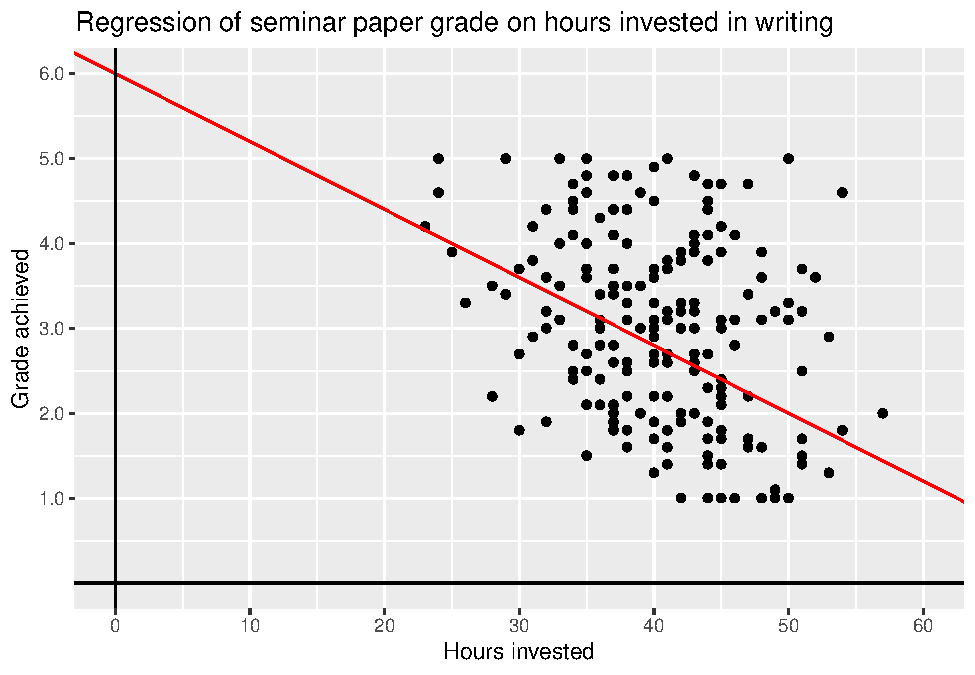
\includegraphics{_main_files/figure-latex/plot_grade_hours_wild_guess_expl_intercept-1.pdf}

We can now see the point where the red line intersects with the y-axis. This is
the intercept of this line, i.e.~\(\beta_0 = 6\).

\[y_{grade} = 6 -0.08*x_{hours} + \epsilon\]

If we now again assume a time investment of \(40\) hours, we can compute
\(6-0.08*40 = 2.8\). So our red regression line - which is still only a wild guess
- assumes, that working 40 hours on a seminar paper will result in a grade of
\(2.8\), on average. We can mark these values in our plot:

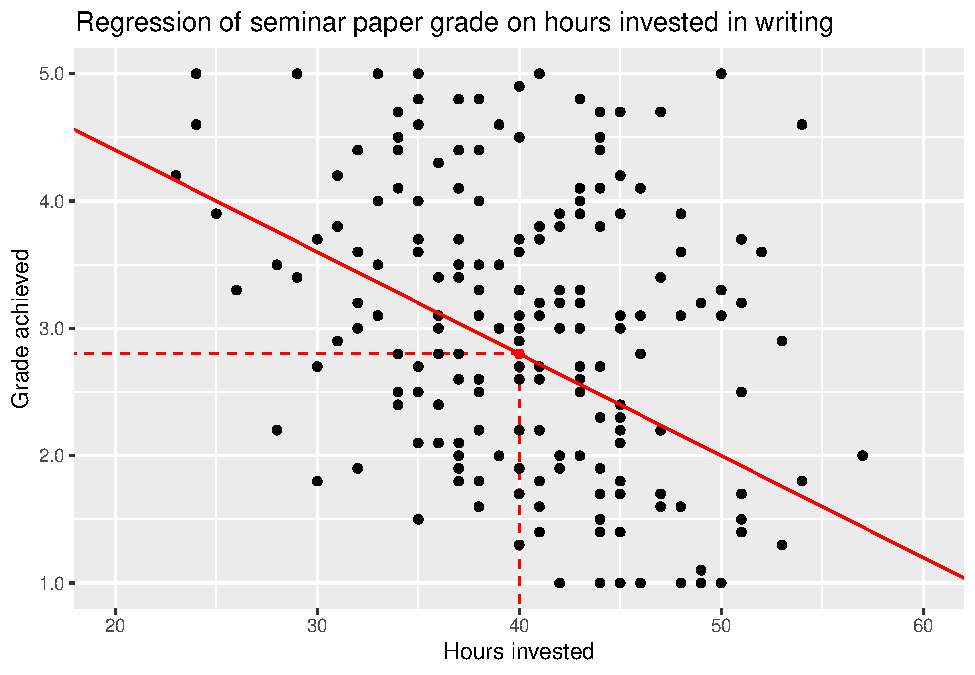
\includegraphics{_main_files/figure-latex/plot_grade_hours_wild_guess_expl_40hours-1.pdf}

The red dot is the intersection of the values \texttt{hours\ =\ 40} and \texttt{grade\ =\ 2.8}.
As this is the value for \(y\) our regression line assumes a student with a time
investment of 40 hours achieves, the red dot also lies exactly on the red line.

But if we look at the plot once again, we can see that most actual observations
for students that invested 40 hours do not actually lie on the regression line
but are scattered above and below the line. Some of these students achieve
much worse or much better grades than \(2.8\) investing the same amount of time in
their work. This leads us to the last part of the formula, \(\epsilon\).

This is the \emph{error term}. Having data that is dispersed like this - and any real
world data will always be - our linear line will never be able to pass exactly
through every data point. Some points may lie exactly on the line, but many or
most will not.

We can visualize this. To keep the plot readable, we only do this for some
random observations but in reality the distance of every data point from the
regression line is taken into account.

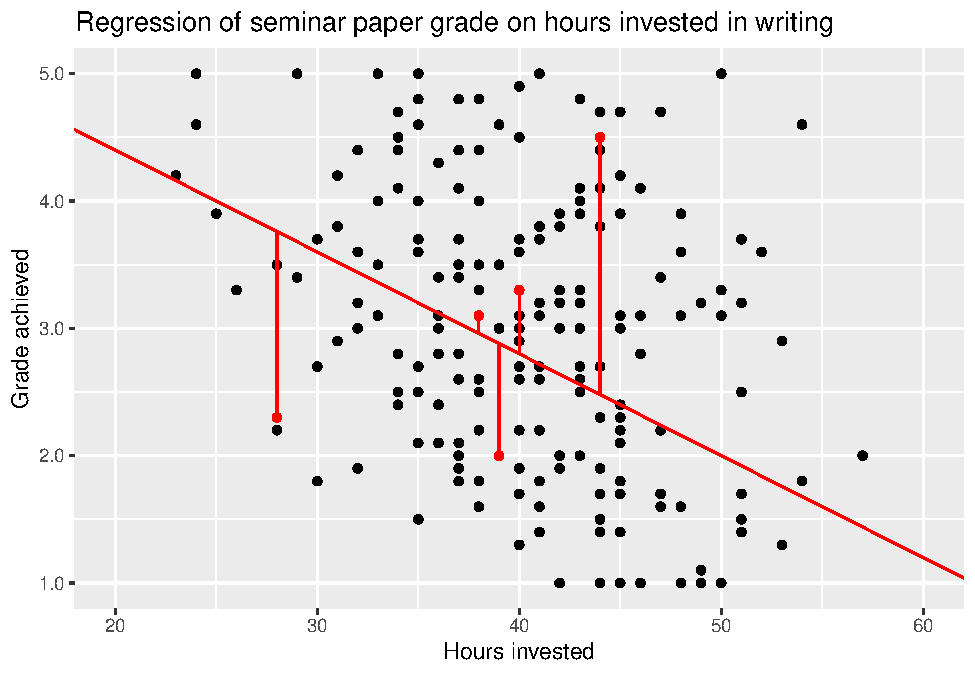
\includegraphics{_main_files/figure-latex/plot_grade_hours_wild_guess_expl_residuals-1.pdf}

The distance of these or rather all points from the line, the \emph{residuals}, are
represented in the error term \(\epsilon\). It is a measure for how wrong our line
is in describing the data in its entirety. So why is it wrong? We can not say
for sure, but there are two common main reasons.

For one, there may be other variables that also influence the relationship
between invested hours and achieved grade, something that we will return to
in the \protect\hyperlink{lin-t-2}{next session}, when we expand the idea of linear regression to multiple
independent variables.

But there is also random variation present in every bit of real world data.
While our data is simulated, we also added random variation on purpose. Because
this is what real world data is, it is messy and it is noisy.

Not every seminar paper that had the same time investment, e.g.~40 hours, will
have the same quality in results. There may be other influential variables, e.g.
the student's general skill level or if they sought assistance by their lecturer
in preparing the paper, influencing the final grade. But even if the quality of
the paper after working 40 hours would be the same for each student, measurement
error, i.e.~noise, will be introduced because not every lecturer will grade
exactly the same or maybe because papers were submitted at different time
points and grading standards may have changed. If we can not measure these
variables we have to accept these unobservable sources of noise and hope, where
\emph{hope} actually means thorough theoretical and methodical thinking, that we can
still measure our effect of interest. This also means, that measuring and
modelling \textbf{always} includes uncertainty. We never know for certain if and to
what extent our results are influenced by unobservable variables and random
variation. Still, there are ways to assess this uncertainty, which we will
regularly return to during the course. This should not stop quantitative
social scientists from making strong or even bold arguments based in thorough
theoretical thinking and responsible data analysis, but we always have to
acknowledge the uncertainty included in every step and make it a part of our
interpretations and conclusions.

The error term \(\epsilon\) is the final piece of the puzzle in actually computing
a linear regression model. Without jumping into the mathematics of it all, the
technique that is used to estimate the coefficients \(\beta_0\) and \(\beta_1\) is
called \emph{OLS} - Ordinary Least Squares. What it basically does, is to take the
squares of all residuals, i.e.~the distances of the data points from the
regression line, sum them up and minimise this value. All this substantially
means is, that OLS searches for the regression line with the lowest amount of error,
i.e.~the lowest overall distance from the actual data points.

OLS gives us estimates for the regression coefficients in this formula:

\[\hat{y} = b_0 +b_1*x_1\]

We can see two differences to the formula we started with. First, we write
\(\hat{y}\) - pronounced as ``y hat'' - instead of \(y\). At the same time, we exclude
the error term \(\epsilon\). This means that we are no longer computing the actual
value of \(y\), as in the point on the regression line for a certain value of
\(x_1\) \(+\) the error, but the estimate \(\hat{y}\), as in the point on the
regression line that is predicted for a certain value of \(x_1\). Second, we write
\(b\) instead of \(\beta\). This also alludes to the fact that we are now
computing an estimate for the coefficients based on the data available and not
the real but unknown value of \(\beta\).

This implies that we now estimate the same grade for every student who invested
the same amount of time, the \(\hat{y}\) that lies exactly on our regression line
at a certain value of \(x_1\). For all students who invested \(40\) hours in writing,
we would estimate exactly the same grade. As we have seen above, these students
received different grades in reality, or more accurately our simulated reality.
The value of \(\hat{y}\) is still the best guess our model can make. That is what
we mean when we say ``on average''. On average a student is estimated to receive
the grade \(\hat{y}\) after investing \(x_1\) hours in writing the paper. We have
to keep in mind, that this will not be true for many students; there is always
an error involved in our estimates.

\hypertarget{regressing-grade-on-hours}{%
\subsection{\texorpdfstring{Regressing \texttt{grade} on \texttt{hours}}{Regressing grade on hours}}\label{regressing-grade-on-hours}}

Now that we have a firmer understanding on what linear regression actually is
and does, we can finally get to the fun part and use the technique for
estimating the effect of \texttt{hours} on \texttt{grade} or in other words, regress
\texttt{grade} on \texttt{hours}.

\begin{verbatim}
## 
## Call:
## lm(formula = grade ~ hours, data = grades)
## 
## Residuals:
##      Min       1Q   Median       3Q      Max 
## -1.88006 -0.83961 -0.08006  0.77006  2.53881 
## 
## Coefficients:
##             Estimate Std. Error t value Pr(>|t|)    
## (Intercept)  5.07912    0.47306  10.737  < 2e-16 ***
## hours       -0.05236    0.01159  -4.517 1.07e-05 ***
## ---
## Signif. codes:  0 '***' 0.001 '**' 0.01 '*' 0.05 '.' 0.1 ' ' 1
## 
## Residual standard error: 1.028 on 198 degrees of freedom
## Multiple R-squared:  0.09344,    Adjusted R-squared:  0.08886 
## F-statistic: 20.41 on 1 and 198 DF,  p-value: 1.075e-05
\end{verbatim}

This is the output from a simple linear regression for \texttt{grade} on \texttt{hours} R
returns to us.
How we can do this in practice and what the first two lines mean will be the
topic of \protect\hyperlink{lin-a}{session 8}. For now we will focus on the estimates in the coefficient
block and introduce the additional elements of the output on by one over the
next sessions.

The column \texttt{Estimate} gives us the values for \(\beta_0\) and \(\beta_1\) discussed
above. The estimated coefficient for \texttt{hours} tells us that out intuition was
right, the more hours a student invests in writing a paper, the better the grade
will be. In this case every additional hour spent on working is estimated to decrease the
value of the grade by \(-0.05236\) points. In keeping with the example of a 40
hour workload this leads to a decrease of \(-0.05236 * 40 = -2.0944\) points.
Adding the intercept from the same column, the estimated grade after working 40
hours is \(5.07912 -0.05236 * 40 = 2.98472\). So on average a student from our
simulated data set will pass after 40 hours of work but will not get a great
grade.
Remember, this is the expected average value. This does not mean that some
students will not get better or worse grades, or even fail to pass with this
amount of time investment.

Now that we know the coefficients for the regression line with the best fit,
i.e.~the lowest error, we can again visualise the result.

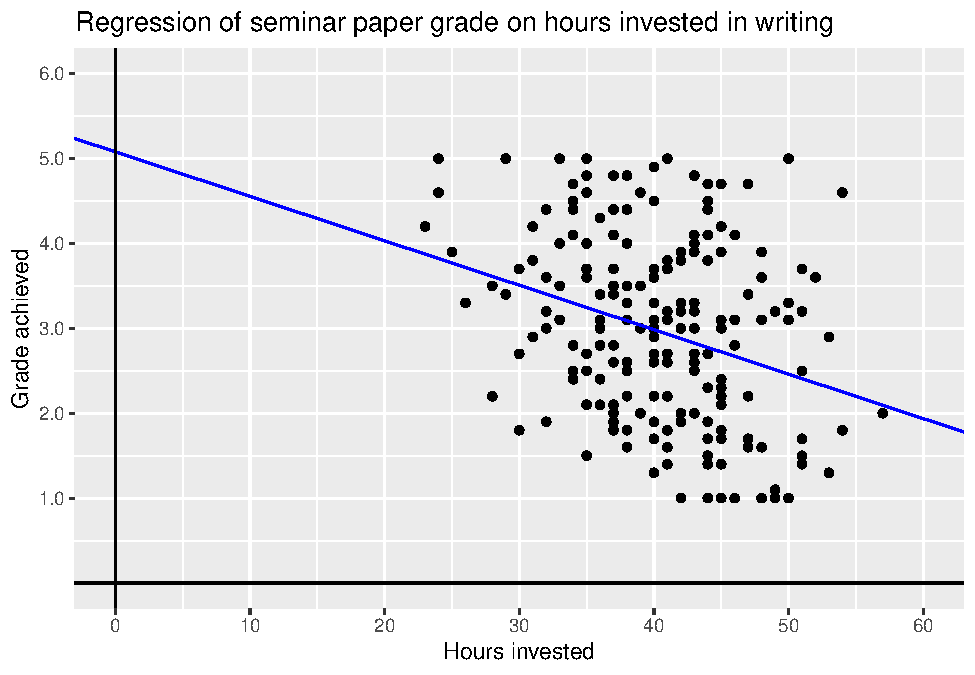
\includegraphics{_main_files/figure-latex/plot_lm_grade_hours-1.pdf}

What grade can a student expect, on average, if they invest exactly 0
hours, i.e.~do nothing and hand in a blank paper. We can look at the graph or,
to achieve a more precise result, calculate it.

\[5.07912 -0.05236 * 0 = 5.07912\]

For this theoretical example of \(x_{hours} = 0\), the estimated value \(\hat{y}\)
or \(y_{grade}\) is the same as the intercept \(\beta_0\). This is what the
intercept represents in general, the estimated value \(\hat{y}\) when the
dependent variable equals \(0\).

Investing zero hours in a seminar paper is not only not advisable, it is
also not a value we observed in our data. If the data would include observations
with zero hours of time invested, the grade would be a firm \(5.0\) and the same
would be true for low single digits, i.e.~turning in a two-pager as a seminar
paper. The takeaway is, that the model is highly dependent on the data that it
is trained on. If the data would have included such cases we could expect a
higher intercept and a steeper slope, i.e.~a stronger negative coefficient.

Luckily all our simulated students have put in at least some hours. But as we do
not have data for zero to \(22\) hours, we can not really make reliable estimates
in this range. Because of this, it does not really make sense to enter \texttt{hours}
into the regression model as ranging from \(0\) to \(57\). One solution that is
often used for metric variables is to center them on their mean. This can be
achieved by simply subtracting the mean of \(x\) from each individual value:

\[x_i - \bar{x}\]

We can now rerun the regression.

\begin{verbatim}
## 
## Call:
## lm(formula = grade ~ hours_centered, data = grades)
## 
## Residuals:
##      Min       1Q   Median       3Q      Max 
## -1.88006 -0.83961 -0.08006  0.77006  2.53881 
## 
## Coefficients:
##                Estimate Std. Error t value Pr(>|t|)    
## (Intercept)     2.96750    0.07267  40.835  < 2e-16 ***
## hours_centered -0.05236    0.01159  -4.517 1.07e-05 ***
## ---
## Signif. codes:  0 '***' 0.001 '**' 0.01 '*' 0.05 '.' 0.1 ' ' 1
## 
## Residual standard error: 1.028 on 198 degrees of freedom
## Multiple R-squared:  0.09344,    Adjusted R-squared:  0.08886 
## F-statistic: 20.41 on 1 and 198 DF,  p-value: 1.075e-05
\end{verbatim}

Comparing the results to the first model shows us, that the coefficient for
\(b_{hours\_centered}\) is exactly the same as for \(b_{hours}\). So the effect
of working more hours has not changed. What has changed is the value of the
intercept. This will make more sense if we again plot the regression line.

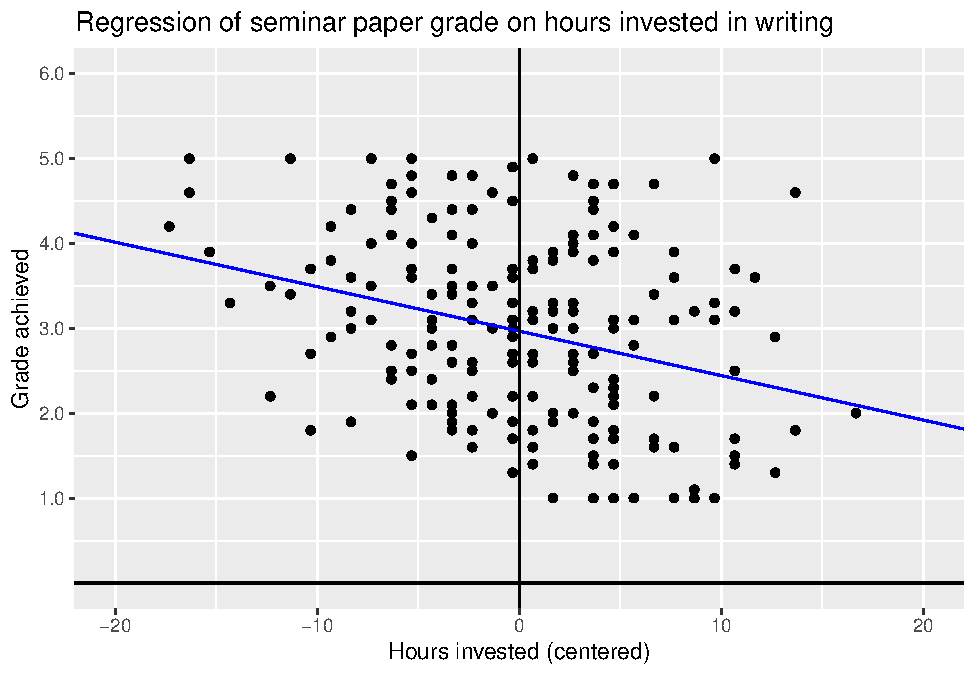
\includegraphics{_main_files/figure-latex/plot_lm_grade_hours_centered_0-1.pdf}

By centering the x-Variable on its mean we have changed its interpretation.
A value of \texttt{hours\ =\ 0} now stands for investing as much time as the mean
of \texttt{hours} in the whole data set, which in this case is \(40.33\) hours. Positive
values indicate that a student worked \(x\) hours more, negatives indicate \(-x\)
hours less compared to the mean. In this way, we also moved the y-axis and thus
changed the interpretation of the intercept. Its new value of \(2.9675\) now
indicates the estimate for a student who invests the mean value of \texttt{hours} in
their work, i.e.~\(40.33\).

\hypertarget{moving-on-1}{%
\section{Moving on}\label{moving-on-1}}

Based on our simple linear regression model we achieved an estimate for our
effect of interest. Working more hours results in receiving a better grade.
But there could be other variables that influence this relationship. In the
\protect\hyperlink{lin-t-2}{next session} we learn how we can include these in our model, when we move from
simple to multiple linear regression.

\hypertarget{lin-t-2}{%
\chapter{Linear Regression - Theory II: Multiple Linear Regression}\label{lin-t-2}}

Maybe explaining the grade a student receives solely based on the hours of
invested time does not paint the whole picture. As we have alluded to, there
may be other variables that could affect the relationship between \texttt{hours} and
\texttt{grade}.
If we fail to include these in our model, we may not get an unbiased estimate
for our effect of interest. Maybe the actual effect for \texttt{hours} is even stronger,
maybe it is weaker, or maybe there is no effect at all.
To assess this, we have to move from simple to multiple linear regression.

\hypertarget{objectives-3}{%
\section{Objectives}\label{objectives-3}}

\begin{itemize}
\tightlist
\item
  Expand the idea to multiple linear regression
\item
  Interpreting different types of independent variables
\item
  Understand measures of uncertainty
\end{itemize}

\hypertarget{multiple-linear-regression}{%
\section{Multiple Linear Regression}\label{multiple-linear-regression}}

A \emph{simple linear regression} only allows for one independent variable. This is
why we need \emph{multiple linear regression} if we want to start introducing
additional variables into the model. Luckily this is easy to understand as we
already know the formula for a simple linear regression:

\[y = \beta_0 + \beta_1*x_1 + \epsilon\]

To change a simple into a multiple linear regression, we just start adding the
additional variables and their coefficients additively to the formula.

\[y = \beta_0 + \beta_1*x_1 + \beta_2*x_2 + ... + \beta_k*x_k + \epsilon\]

So to add a second variable and its coefficient we add the term \(+ \beta_2*x_2\)
and so on until we added all independent variables of interest \(k\) to the model.
Everything else works exactly as for the simple model.

\hypertarget{adding-additional-metric-variables}{%
\subsection{Adding additional metric variables}\label{adding-additional-metric-variables}}

We already expected that the mean of the previous grades could be a strong
predictor for future grades. We could understand these as a \emph{proxy} variable for
the general skill level of a student. The higher the skill level, the higher
previous grades will have been.

How we can add additional variables in R code will again be a topic for the next
session, but let us look at the results of a regression of \texttt{grade} on
\texttt{hours\_centered} and \texttt{previous\_grades\_centered}, the latter being centered on the
mean previous grade of \(2.935\).

\begin{verbatim}
## 
## Call:
## lm(formula = grade ~ hours_centered + previous_grades_centered, 
##     data = grades)
## 
## Residuals:
##      Min       1Q   Median       3Q      Max 
## -1.44462 -0.30556  0.00622  0.32878  1.31002 
## 
## Coefficients:
##                           Estimate Std. Error t value Pr(>|t|)    
## (Intercept)               2.967500   0.038316  77.449   <2e-16 ***
## hours_centered           -0.056543   0.006114  -9.248   <2e-16 ***
## previous_grades_centered  0.904079   0.039830  22.699   <2e-16 ***
## ---
## Signif. codes:  0 '***' 0.001 '**' 0.01 '*' 0.05 '.' 0.1 ' ' 1
## 
## Residual standard error: 0.5419 on 197 degrees of freedom
## Multiple R-squared:  0.7492, Adjusted R-squared:  0.7467 
## F-statistic: 294.3 on 2 and 197 DF,  p-value: < 2.2e-16
\end{verbatim}

As we added a new variable, we now see three coefficients.
The intercept has not changed. It now indicates the estimated grade for a
student who invests the mean amount of hours, \(40.33\), and whose previous grades
are exactly \(2.935\), the mean of the variable.

The coefficient for \texttt{hours\_centered} got mildly more negative, still telling us
that the value of \texttt{grade} gets lower, the more hours are invested in writing the
paper. This coefficient now gives us the effect while \emph{controlling} for the
effect of \texttt{previous\_grades\_centered}. This is what multiple linear regression
does, giving us the coefficients for our variables of interest while keeping all
other independent variables at specific values. As we have centered the variable
for previous grades, the coefficient for \texttt{hours\ centered} gives us the effect
when the previous grades were exactly at the mean of \(2.935\).

In the same way, the coefficient for \texttt{previous\_grades\_centered} gives us the
effect of previous grades when the invested hours are controlled for, in this
case when the invested hours were exactly \(40.33\). The coefficient is rather
high and positive. This indicates that a student with a previous grade value
that is \(1\) above the mean, is estimated to receive a new grade that is \(0.9\)
points above the intercept. This means, that the previous grade is a very strong
predictor for the new grade.

While plotting in more than two dimensions gets really hard, we can still
calculate \(\hat{y}\) for certain values of both independent variables.
We already know the predicted grade for a student with mean values on both
independent variables, as this is the intercept. To make sure that we correct,
we can calculate it again.

\[b_0 + b_{hours\_centered}*0 + b_{previous\_grades\_centered}*0 = 2.9675\]

For this case we can see that the previous grade actually is a strong
predictor, as the previous and new grades are substantially the same.

What if a student whose previous grades were \(1\) above the mean, so just below
\(4.0\), but who decides to invest \(10\) hours more than the mean in writing the new paper?

\[2.9675 - 0.056543 * 10 + 0.904079 * 1 = 3.306149\]

So the good message is, while previous grades are a strong predictor, putting in
more hours still leads to better grades.

What if a really good student decides to rely on their skill and to work less
this time?

\[2.9675 - 0.056543 * -10 + 0.904079 * -2 = 1.724772\]

While \(1.7\) is still a very good grade, working 10 less hours than the mean of
students leads to a substantially worse estimate compared to the about \(1.0\)
received in previous grades.

\hypertarget{adding-dummy-variables}{%
\subsection{Adding dummy variables}\label{adding-dummy-variables}}

Another variable that could be of interest in explaining the received grade,
is if a student attended most of the seminar sessions.
\texttt{attendance} holds this information in the form of a dummy variable. Dummies can
only have two states. ``Yes'' or ``No'', ``1'' or ``0'' or in this case ``\texttt{TRUE}'' or
``\texttt{FALSE}''.

Let us add the variable to our model.

\begin{verbatim}
## 
## Call:
## lm(formula = grade ~ hours_centered + previous_grades_centered + 
##     attendance, data = grades)
## 
## Residuals:
##      Min       1Q   Median       3Q      Max 
## -1.41059 -0.30910  0.01667  0.35607  1.29849 
## 
## Coefficients:
##                           Estimate Std. Error t value Pr(>|t|)    
## (Intercept)               3.157411   0.078658  40.141  < 2e-16 ***
## hours_centered           -0.053942   0.006088  -8.860 4.85e-16 ***
## previous_grades_centered  0.911802   0.039282  23.212  < 2e-16 ***
## attendanceTRUE           -0.248250   0.090246  -2.751   0.0065 ** 
## ---
## Signif. codes:  0 '***' 0.001 '**' 0.01 '*' 0.05 '.' 0.1 ' ' 1
## 
## Residual standard error: 0.5331 on 196 degrees of freedom
## Multiple R-squared:  0.7586, Adjusted R-squared:  0.7549 
## F-statistic: 205.3 on 3 and 196 DF,  p-value: < 2.2e-16
\end{verbatim}

This gives us a new line in the R Output holding an estimate for
\texttt{attendanceTRUE}. What is meant by this? In contrast to the metric variables we
have uses in our model up to this point, a dummy variable - or binary variable -
can only have two states. As we are using a logical variable here, it can only
have the value \texttt{TRUE} - here indicating regular attendance - or \texttt{FALSE}. So what
the output shows us, is the effect of attendance being \texttt{TRUE} compared to being
\texttt{FALSE}. If a student did regularly attend the seminar, the estimated grade is
\(-0.248250\) lower compared to when they did not.

We can observe what happens in the formula:

\[\hat{y} = b_0 + b_{hours\_centered}*x_{hours\_centered} + \\
b_{previous\_grades\_centered} * x_{previous\_grades\_centered} +\\ 
b_{attendance} * x_{attendance}\]

If you calculate with \texttt{TRUE} and \texttt{FALSE} in R, the values \(1\) and \(0\) are used
respectively. So \(x_{attendance}\) can either have the value \(1\) for regular
attendance or \(0\) for not so regular attendance.

If a student did regularly attend, the coefficient \$b\_\{attendance\} becomes a
part of the estimate \(\hat{y}\):

\[\hat{y} = b_0 + b_{hours\_centered}*x_{hours\_centered} +\\
b_{previous\_grades\_centered}*x_{previous\_grades\_centered} +\\ 
b_{attendance} * 1\]

If student did not regularly attended, this happens:

\[\hat{y} = b_0 + b_{hours\_centered}*x_{hours\_centered} \\
+ b_{previous\_grades\_centered}*x_{previous\_grades\_centered} +\\
b_{attendance} * 0\]

Which shortens to:

\[\hat{y} = b_0 + b_{hours\_centered}*x_{hours\_centered} +\\
b_{previous\_grades\_centered}*x_{previous\_grades\_centered}\]

The coefficient is no longer a part of the estimate. One can basically say, the
coefficient gets switched on or off by the value of the dummy variable.

So while the estimate for a student with mean values for invested hours and
previous grades who did not attend is equal to the intercept of \(3.157411\),
for a similar student who attended we can calculate the estimate as:

\[3.157411 - 0.053942*0 + 0.911802*0 - 0.248250 * 1 = 3.157411 - 0.248250 \\
= 2.909161\]

It seems attending class is an easy way to raise one's grades.

\hypertarget{adding-categorical-variables}{%
\subsection{Adding categorical variables}\label{adding-categorical-variables}}

We have one further variable in our simulated data set that could be of interest
in explaining, what makes a good grade in a seminar paper. \texttt{contact} is a
categorical variable, or a factor variable in R terms.
It can take three different categories. \texttt{No\ contact} indicates that
the student did not contact the lecturer to discuss a research question or the
laid out plan for the paper. \texttt{E-Mail} means that there was some written contact
and at least the basics for the paper were discussed before writing. Lastly,
\texttt{In\ Person} stands for an in depth discussion with the lecturer, clearing up
problems beforehand and thus potentially having a more stringent vision for the
paper before writing the first word.

Let us add the variable to our model.

\begin{verbatim}
## 
## Call:
## lm(formula = grade ~ hours_centered + previous_grades_centered + 
##     attendance + contact, data = grades)
## 
## Residuals:
##     Min      1Q  Median      3Q     Max 
## -1.3835 -0.2525  0.0167  0.2678  0.9347 
## 
## Coefficients:
##                           Estimate Std. Error t value Pr(>|t|)    
## (Intercept)               3.617949   0.068077  53.145  < 2e-16 ***
## hours_centered           -0.050830   0.004433 -11.466  < 2e-16 ***
## previous_grades_centered  0.874123   0.028657  30.503  < 2e-16 ***
## attendanceTRUE           -0.324653   0.065781  -4.935 1.72e-06 ***
## contactE-Mail            -0.413808   0.069817  -5.927 1.39e-08 ***
## contactIn Person         -0.853252   0.063964 -13.340  < 2e-16 ***
## ---
## Signif. codes:  0 '***' 0.001 '**' 0.01 '*' 0.05 '.' 0.1 ' ' 1
## 
## Residual standard error: 0.3869 on 194 degrees of freedom
## Multiple R-squared:  0.8741, Adjusted R-squared:  0.8709 
## F-statistic: 269.4 on 5 and 194 DF,  p-value: < 2.2e-16
\end{verbatim}

Wait, we entered three categories into the model and got estimates for two of
them. What happened? What R does is to create two dummy variables on the fly.
The first discerns between having E-Mail contact and no contact at all. The
second one between having contact in person and no contact at all. So for
categorical variables in regression models we always compare being in one of the
categories to being in the \emph{base category}. In this case the base category is
\texttt{No\ contact}, but we could also change the base category. It depends on what we
are interested in comparing to. For our example comparing the effects of having
more in depth contact to having none makes sense.

Let us look at our formula again:

\[\hat{y} = b_0 + b_{hours\_centered}*x_{hours\_centered} +\\
b_{previous\_grades\_centered} * x_{previous\_grades\_centeerd} +\\
b_{attendance} * x_{attendance} +\\
b_{E-Mail} * x_{E-Mail} + b_{In Person} * x_{In Person}\]

Now there are three possibilities. A student can have no contact at all. In this
case both dummy variables are equal to \(0\). To make our formula easier to read, we have
abbreviated the middle part for now:

\[\hat{y} = b_0 + ... + b_{E-Mail} * 0 + b_{In Person} * 0\]

So in this case controlling all other independent variables at their default
values, the mean for the metric variables and \texttt{FALSE} for \texttt{attendance}, the
intercept gives us the estimate for the grade when the student had no contact to
the lecturer, as both dummy variables that were created for \texttt{contact} are ``switched off''.

The two other possibilities are that a student either had E-Mail contact or an
in person discussion:

\[\hat{y} = b_0 + ... + b_{E-Mail} * 1 + b_{In Person} * 0\]

\[\hat{y} = b_0 + ... + b_{E-Mail} * 0 + b_{In Person} * 1\]

In both cases the relevant dummy variable is ``switched on'' while the other does
not factor into the equation.

Looking at the estimates we can see that having contact to the lecturer before
writing has strong negative effects, resulting in better grades. Having E-Mail
contact reduces the value of \texttt{grade} by \(-0.413808\) points, having an in person
discussion by \(-0.853252\).

So what grade can a student whose previous grades were at the mean of \(2.935\),
but who decided to put in 20 hours more compared to their peers, regularly
attend the seminar and have an in-depth personal discussion before writing their
paper expect on average as their new grade?

\[3.617949 - 0.050830 * 20 + 0.874123 * 0 - 0.324653 * 1 - 0.413808 * 0 - 0.853252 * 1 
\\ = 1.423444\]

Putting in the hours, attending and working with your lecturer seems to pay off,
at least in our simulated data set.

\hypertarget{returning-to-our-research-question}{%
\section{Returning to our research question}\label{returning-to-our-research-question}}

Our exemplary research question concerned itself with what makes a good grade in
a seminar paper. In particular we were interested in the effect of the invested
hours, as our main hypothesis was that more hours lead to better grades. What do
we know now?

Our analysis points towards a clear effect from \texttt{hours} on \texttt{grade}. This effect
was consistently visible in all of our models. But did we correctly identify
and estimate the effect of interest? Maybe. The problem is, we actually did not
approach the analysis correctly. In a real analysis we should \textbf{absolutely}
refrain from adding variables to our model that \emph{could be} relevant until we are
satisfied or even until all available variables are bunched into one huge model.
It was fine to do this in this introduction to linear regression to learn how
different types of variables can be used in a regression model. But in a real
project, we have to invest time to think about which variables to add because we
assume that they have a relevant effect based on theoretical assumptions about
the processes we are interested in.

So let us do this now and vow do make this our first step in all future
endeavors. While we do not have a clear theoretical basis, we can make clear
assumptions on the data generating process and draw these in a DAG.

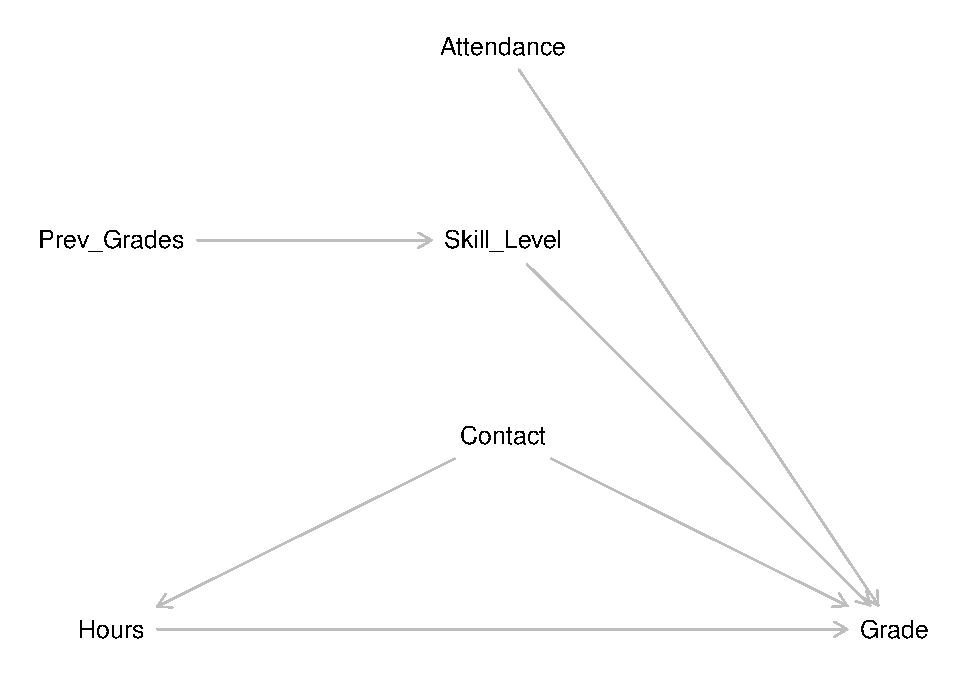
\includegraphics{_main_files/figure-latex/dag-1.pdf}

Our central assumption, and the effect we want to identify and estimate, is the
direct effect from \texttt{hours} on \texttt{grade} in the bottom line. The more hours a
student invests, the better the grade should be.

The assumed effect of \texttt{contact} is more complex. For one we assume that a more
in-depth contact with the lecturer will increase the grade directly. The
research question will be more focused, the student will know what is important
to a certain lecturer, common mistakes can be avoided if they are cleared up
beforehand and so on. But we will also assume that \texttt{contact} will have an effect
on \texttt{hours} in the sense that the hours invested can be used more efficiently if
an in-depth discussion has taken place. Instead of wasting time running into
problems that could have been avoided most of the invested time can actually go
into constructive work. This makes \texttt{contact} a confounder for \texttt{grade} and
\texttt{hours}.

A student's skill level will also have a direct effect on \texttt{grade}. As we do not
have a direct measure of skill in our data, we use \texttt{previous\_grades} as a proxy
for skill level. \texttt{attendance} is also assumed to have a direct effect on \texttt{grade}
as students who were present in the seminar will not only have learned the seminar's
contents, but will also have a better understanding of what is expected in their
seminar papers.

Tapping into the knowledge from session 4, we can now make implications for our
model from the DAG. Let us list all paths from \texttt{hours} to \texttt{grade}:

\[A: Hours \rightarrow Grade\]

\[B: Hours \leftarrow Contact \rightarrow Grade\]

Path A represents our effect of interest. On path B, \texttt{contact} is a confounder
for \texttt{hours} and \texttt{grade}. To close this path, we have to control for \texttt{contact}.
As neither skill level - or \texttt{previous\_grades} - nor \texttt{attendance} lie on a path
from our independent variable of interest to our dependent variable, we should
not control for them in our model.
That leaves us with \texttt{hours} and \texttt{contact} to be included in our linear
regression, if our goal is to get an unbiased estimate for the effect of
invested time on the final grade. So let us do this:

\begin{verbatim}
## 
## Call:
## lm(formula = grade ~ hours_centered + contact, data = grades)
## 
## Residuals:
##      Min       1Q   Median       3Q      Max 
## -1.85595 -0.74624 -0.02106  0.66648  2.50161 
## 
## Coefficients:
##                  Estimate Std. Error t value Pr(>|t|)    
## (Intercept)       3.44352    0.10404  33.098  < 2e-16 ***
## hours_centered   -0.04967    0.01052  -4.723 4.43e-06 ***
## contactE-Mail    -0.46482    0.16785  -2.769  0.00616 ** 
## contactIn Person -1.02804    0.15240  -6.746 1.67e-10 ***
## ---
## Signif. codes:  0 '***' 0.001 '**' 0.01 '*' 0.05 '.' 0.1 ' ' 1
## 
## Residual standard error: 0.9305 on 196 degrees of freedom
## Multiple R-squared:  0.2643, Adjusted R-squared:  0.253 
## F-statistic: 23.47 on 3 and 196 DF,  p-value: 5.072e-13
\end{verbatim}

This is our estimate. Each hour invested beyond the mean of \(40.33\) hours
changes the grade by about \(-0.05\) points. This supports our hypotheses and we
can conclude, that investing more hours into writing a seminar paper actually
is a worthwhile investment.

But remember: This is correct as long as our DAG is drawn correctly, which is
always debatable. Maybe we should assume an effect from skill level on \texttt{hours}.
The higher the skill level the more efficiently the available time can be used.
For this example we know the DAG is correct, because we have simulated the data
exactly in this way. For real world applications we never know if our DAG is
correct. All we can and \emph{have to} do is base it on thorough thinking,
theoretical work, exploratory data analysis and sound arguments.

This all is true \emph{if} our goal is to estimate an effect of interest as precisely
as possible. But as we have alluded to in the introduction to this session we
could also use modelling with a different goal, i.e.~predicting a grade as
accurately as possible. For this task, the model which only includes \texttt{hours} and
\texttt{contact} will not do the best job. From our DAG we know that \texttt{attendance} and
\texttt{previous\_grade} should have an effect on \texttt{grade}, as we have also seen in our
models. For this task the full model including all these variables will produce
better estimates. We will return to this in a later session, but for now we
should remember that we have to know our task because the task dictates which is
the best model to use.

\hypertarget{adressing-the-uncertainty}{%
\section{Adressing the uncertainty}\label{adressing-the-uncertainty}}

Looking at the coefficient block from the output, we see more
than just our estimates. The \texttt{Std.\ Error} - \emph{standard error} - is a measure for the
uncertainty of our estimates. It basically tells us, how far away the actual
values of the observations used to compute the model are from our estimate
\emph{on average}. The smaller the \emph{standard error}, the more accurate our
estimate. The standard error is presented in the units of the estimate and we
can thus compare them. A large standard error for a large estimate is far less
problematic compared to a large standard error for a small estimate.

The estimate and it's standard error are the basis for \emph{hypothesis testing}.
What we are testing is the \emph{alternative hypotheses} \(H_a\) that there actually
is an effect of our independent variable on the dependent variable against the
\emph{null hypothesis} \(H_0\) that there is no effect. To reject the null hypothesis
and be confident that we are observing an actual effect, versus an effect that
is just based on random variation in our sample, the estimate has to be far
away enough from \(0\) and be accurate enough, i.e.~have a small standard error.
This relationship is computed in the \emph{t-statistic}, \texttt{t\ value} in
our output. From this the \emph{p-value} can be computed, \texttt{Pr(\textgreater{}\textbar{}t\textbar{})} in the output.
The \emph{p-value} tells us the probability to observe an association
between the independent and the dependent variable as large or larger than our
estimate suggests, if the true association would actually be \(0\). If the p-value
is small enough, we can reject \(H_0\) and conclude that we observed an actual
effect. There are certain agreed upon cutoffs in statistics, while values that
meet this cutoffs are considered \emph{statistically significant}. The most common
cutoff in social sciences is \(0.05\) indicated by one \texttt{*} in the output.
Other common cutoffs are indicated by more asterisks. It is important to note,
that we can not say that more \texttt{*} behind an effect mean that this effect has a
higher statistical significance. We have to decide on a level of statistical
significance that we want to test for before we see the results. If we decide on
testing for a significance level of \(5\%\), seeing more than one star then only
means that the effect is also statistically significant at the \(5\%\) level.

Interpreting p-values correctly and not falling into the common pitfalls like the
one mentioned above is a
topic on its own. We do not have the time to dive into this here, so for now we
can agree that p-values below \(0.05\) indicate that we can reject \(H_0\) and thus
conclude that we have actually observed an effect. Still, our interpretation of
regression results should not focus solely on p-values or lead us to disregard
any effects that did not meet the cutoff. For example, we can have very small
p-values for effects that are so small that they are substantially irrelevant.
One way to address this is to inspect the actual magnitudes of the effects.
On the other hand, we
can have p-values larger than \(0.05\) for effects that are still relevant. Maybe
the problem is not that there is no effect but that we were not able to measure
the variable in question precisely enough or that we just did not have enough
observations. We can not go any deeper than this here, but we should remember
that the practice of declaring every effect with stars a win, or even with more
stars a bigger win, and disregarding
everything without them may still be common but is not the way to go forward.

In our model, we can see that the effect of interest is statistically
significant. We can thus conclude, that we have observed an actual effect
from \texttt{hours} on \texttt{grade}. Our estimate is large enough and our standard error
small enough to reach this conclusion.

\hypertarget{moving-on-2}{%
\section{Moving on}\label{moving-on-2}}

We have attained an estimate for our effect of interest which supports our
hypotheses that investing more hours into writing a paper leads to better grades.
So can we wrap a bow on the question and move on to finally figuring out what
is going on in our NBA data? Almost, but not yet. We still do not know, if our
model actually works as intended. Linear regression, as well as every other modelling
technique, has some underlying statistical assumptions that we have to meet for the model
to accurately estimate an effect. In the \protect\hyperlink{lin-t-3}{next session} we will get to know these
assumptions and how we can test for them.

\hypertarget{lin-t-3}{%
\chapter{Linear Regression - Theory III: Diagnostics}\label{lin-t-3}}

In this session we will get to know the central underlying assumptions for linear regression models. To find out if our model actually works as intended and thus gives us a reliable estimate for the effect of \texttt{hours} on \texttt{grade}, we have to check if we have met these assumptions, and if we did not, we have to correct our model accordingly. Before we do this, we should briefly consider another part of the regression output, the model fit.

\hypertarget{objectives-4}{%
\section{Objectives}\label{objectives-4}}

\begin{itemize}
\tightlist
\item
  Learn about model fit and its limits
\item
  Understand the statistical assumptions underlying linear regression
\item
  Test for violated assumptions and learn how to correct for those
\end{itemize}

\hypertarget{model-fit}{%
\section{Model fit}\label{model-fit}}

Let us again inspect the output from the simplest model we computed, regressing the grade solely on the invested hours:

\begin{verbatim}
## 
## Call:
## lm(formula = grade ~ hours_centered, data = grades)
## 
## Residuals:
##      Min       1Q   Median       3Q      Max 
## -1.88006 -0.83961 -0.08006  0.77006  2.53881 
## 
## Coefficients:
##                Estimate Std. Error t value Pr(>|t|)    
## (Intercept)     2.96750    0.07267  40.835  < 2e-16 ***
## hours_centered -0.05236    0.01159  -4.517 1.07e-05 ***
## ---
## Signif. codes:  0 '***' 0.001 '**' 0.01 '*' 0.05 '.' 0.1 ' ' 1
## 
## Residual standard error: 1.028 on 198 degrees of freedom
## Multiple R-squared:  0.09344,    Adjusted R-squared:  0.08886 
## F-statistic: 20.41 on 1 and 198 DF,  p-value: 1.075e-05
\end{verbatim}

Up to now, we exclusively talked about the coefficient block. We will return to the ``Call'' \protect\hyperlink{lin-a}{next session} and to the ``Residuals'' later in this session. For now let us focus on the bottom block in the output.

\(R^2\) or \emph{R-squared} is a measure for the amount of variance in the data that is ``explained'' by the model. Real world data will always have variance. Not every value will neatly fall onto the mean value of a variable. Rather the data is dispersed around it. The same is true for our dependent variable:

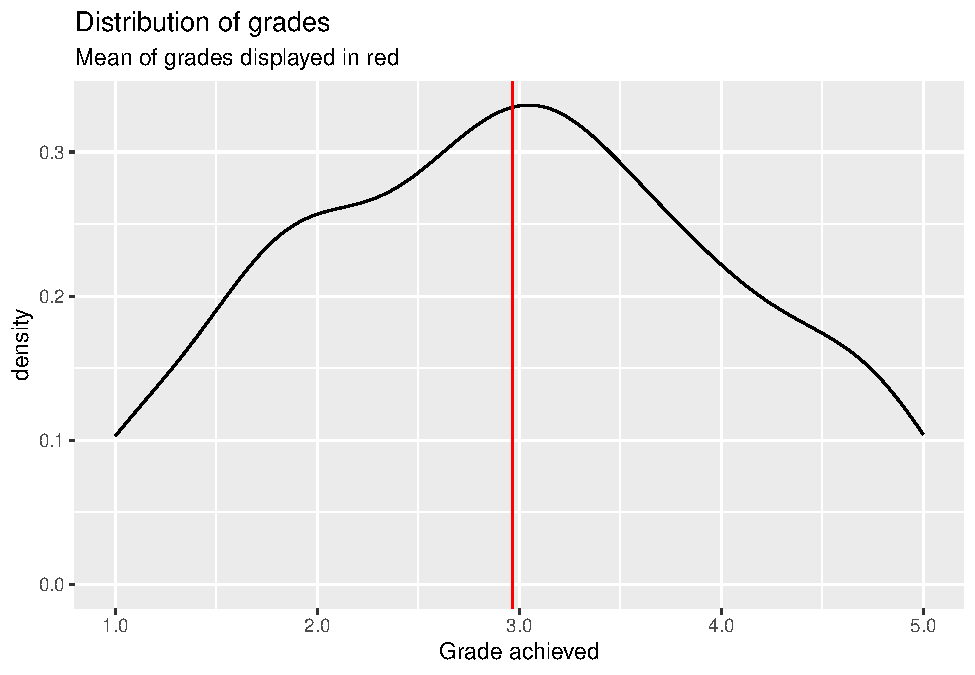
\includegraphics{_main_files/figure-latex/plot_grade_distribution-1.pdf}

This is a density plot and shows the distribution of a metric variable as a smoothed line. We do not see every individual actual value but the general shape of the data. The red line represent the mean of \texttt{grade}, which is about \(2.97\). Most actual values are not exactly at the mean but are rather dispersed around it, ranging between \(1.0\) and \(5.0\). This is the variance in our outcome variable.

Let us now plot \texttt{grade} against \texttt{hours\_centered} and add the regression line from our model above:

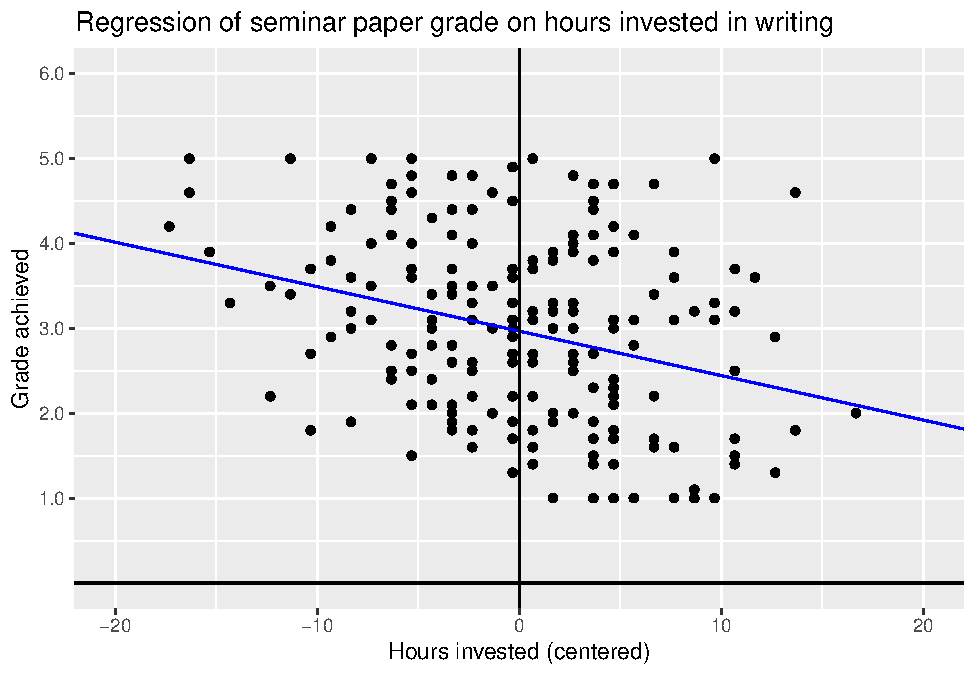
\includegraphics{_main_files/figure-latex/plot_lm_grade_hours_centered-1.pdf}

Without our regression line, all we would have is a cloud of points without much order to it. What linear regression does, is trying to bring order into this by fitting a line that best explains the variance of the dependent variable, \texttt{grade} in our case by its relationship to one or multiple dependent variables, here \texttt{hours\_centered}. But this linear line can never explain the variance completely. For this it had to pass through every data point. Our line does not. Actually most data points do not lie on the regression line but at some distance to it. You will remember that OLS computes \emph{the} regression line for which the squared distances are smallest. This is the line that explains most of the variance of \(y\) by its relationship to \(x\), but not all variance is explained. An unexplained part remains. These are the residuals; the distance that points fall from the regression line. \(R^2\) tells us the relative amount of how much we reduced the initial variance by fitting the line and thus explaining a part of said variance.

A \(R^2\) of \(0\) would mean that no variance is explained, a value of \(1\) that all variance is explained. Two highly unlikely outcomes. We will almost always explain something and never explain everything.

In our model \(R^2\) equals \(0.09344\). This means we explained about \(9.3\%\) of the variance of \texttt{grade} by its relationship with \texttt{hours\_centered}. That's nice, but this also means that over \(90\%\) are still unexplained. We will not explain all of the variance, i.e.~\(R^2 = 1\), but in general a higher \(R^2\) is desirable.

So what can we do? We can try to add additional variables to the model that help in explaining the variance of the outcome variable. Last session we concluded that the best model to measure the effect of invested hours on the achieved grade would also have to include \texttt{contact}:

\begin{verbatim}
## 
## Call:
## lm(formula = grade ~ hours_centered + contact, data = grades)
## 
## Residuals:
##      Min       1Q   Median       3Q      Max 
## -1.85595 -0.74624 -0.02106  0.66648  2.50161 
## 
## Coefficients:
##                  Estimate Std. Error t value Pr(>|t|)    
## (Intercept)       3.44352    0.10404  33.098  < 2e-16 ***
## hours_centered   -0.04967    0.01052  -4.723 4.43e-06 ***
## contactE-Mail    -0.46482    0.16785  -2.769  0.00616 ** 
## contactIn Person -1.02804    0.15240  -6.746 1.67e-10 ***
## ---
## Signif. codes:  0 '***' 0.001 '**' 0.01 '*' 0.05 '.' 0.1 ' ' 1
## 
## Residual standard error: 0.9305 on 196 degrees of freedom
## Multiple R-squared:  0.2643, Adjusted R-squared:  0.253 
## F-statistic: 23.47 on 3 and 196 DF,  p-value: 5.072e-13
\end{verbatim}

We can use \(R^2\) to compare the \emph{model fit} of multiple models. Here the larger model achieved a considerably higher value of \(R^2 = 0.2643\). The model fit improved as we can now explain a higher ratio of the variance in \texttt{grade}.

After \(R^2\) we see another value, \emph{Adjusted R-squared}. This becomes relevant if we add additional variables to our model. \(R^2\) almost always increases, and never decreases, when adding additional variables to the model, especially if we have few observations. Because of this \(R^2\) can get less reliable when we have many variables and few observations. \emph{Adjusted R-squared} corrects for this by including both factors in the calculation. When we have many observations the differences are negligible. This is true for our case. We have relatively many observations and few variables in our model, so the values of both measures are rather close. But in cases where this relationship is not as favorable, adjusted R-squared should be used in place of the regular \(R^2\).

The block in our output also gives us the \emph{Residual standard error}. As we have seen above, most actual data point do not lie on the regression line but some distance away from it. These are the residuals. Thus their standard error basically tells us how much we miss the spot on average. As it is given in units of the dependent variable, we can say that the estimates for \texttt{grade} based on our second model are on average \(0.93\) off. A considerable amount, as this is almost one whole grading step. This is still an improvement from the \(1.028\) in the first model but nevertheless a substantial error.

The last line in the output gives us two connected measures. The \emph{F-statistic} is the test statistic for \(R^2\) and is used the compute the corresponding \emph{p-value}. In this case we are testing if the \(R^2\) our model returned based on our sample is possible, when the actual population value of \(R^2\) is \(0\). In other words, could we have achieved this \(R^2\) by chance if the independent variables in our model actually do not explain part of the variance in the population? Both of our models have very small p-values, so it is highly unlikely that we have just explained some variance by chance. This gives further credibility to our model specification.

We can conclude that the second model was an improvement over the first. But can we do more? Sure; we can always add additional explanatory variables:

\begin{verbatim}
## 
## Call:
## lm(formula = grade ~ hours_centered + previous_grades_centered + 
##     attendance + contact, data = grades)
## 
## Residuals:
##     Min      1Q  Median      3Q     Max 
## -1.3835 -0.2525  0.0167  0.2678  0.9347 
## 
## Coefficients:
##                           Estimate Std. Error t value Pr(>|t|)    
## (Intercept)               3.617949   0.068077  53.145  < 2e-16 ***
## hours_centered           -0.050830   0.004433 -11.466  < 2e-16 ***
## previous_grades_centered  0.874123   0.028657  30.503  < 2e-16 ***
## attendanceTRUE           -0.324653   0.065781  -4.935 1.72e-06 ***
## contactE-Mail            -0.413808   0.069817  -5.927 1.39e-08 ***
## contactIn Person         -0.853252   0.063964 -13.340  < 2e-16 ***
## ---
## Signif. codes:  0 '***' 0.001 '**' 0.01 '*' 0.05 '.' 0.1 ' ' 1
## 
## Residual standard error: 0.3869 on 194 degrees of freedom
## Multiple R-squared:  0.8741, Adjusted R-squared:  0.8709 
## F-statistic: 269.4 on 5 and 194 DF,  p-value: < 2.2e-16
\end{verbatim}

The p-value is even lower, and the F-statistic even higher, compared to our second model, but this was never an issue. What is more interesting is that we have substantially increased \(R^2\) and decreased the residual standard error. As we have concluded last week, this larger model is better at predicting the actual values of \texttt{grade}. Thus the explained variance has to increase and the average error in estimating \texttt{y} has to decrease. But is this the better model? The values on the model fit would suggest so. And this also is true, if our aim is predicting \texttt{grade} to the best of our abilities. But if our aim is still measuring the effect of \texttt{hours} on \texttt{grade} we know from our DAG that we do not have to or even should not control for the additional variables to get an unbiased estimator for the effect of interest.

What can we take away from this? While the model fit measures are an important tool for comparing multiple possible models and better values are desirable in general, it should not be our goal to just max out all measures and declare this model the ``winner''. It is never that easy in statistics. One thing we can never replace is thorough theoretical work before even computing our first model. Based on our DAG, if it is correct, we know that we do not have to control for previous grades and attendance. Including them may give us a larger \(R^2\), but is still not the correct way to build our model.

Based on this our best model is still the second one:

\begin{Shaded}
\begin{Highlighting}[]
\FunctionTok{summary}\NormalTok{(m2)}
\end{Highlighting}
\end{Shaded}

\begin{verbatim}
## 
## Call:
## lm(formula = grade ~ hours_centered + contact, data = grades)
## 
## Residuals:
##      Min       1Q   Median       3Q      Max 
## -1.85595 -0.74624 -0.02106  0.66648  2.50161 
## 
## Coefficients:
##                  Estimate Std. Error t value Pr(>|t|)    
## (Intercept)       3.44352    0.10404  33.098  < 2e-16 ***
## hours_centered   -0.04967    0.01052  -4.723 4.43e-06 ***
## contactE-Mail    -0.46482    0.16785  -2.769  0.00616 ** 
## contactIn Person -1.02804    0.15240  -6.746 1.67e-10 ***
## ---
## Signif. codes:  0 '***' 0.001 '**' 0.01 '*' 0.05 '.' 0.1 ' ' 1
## 
## Residual standard error: 0.9305 on 196 degrees of freedom
## Multiple R-squared:  0.2643, Adjusted R-squared:  0.253 
## F-statistic: 23.47 on 3 and 196 DF,  p-value: 5.072e-13
\end{verbatim}

\hypertarget{regression-diagnostics}{%
\section{Regression diagnostics}\label{regression-diagnostics}}

As linear regression is a statistical technique, there are certain statistical assumptions we have to meet. If we violate those, the best laid plans may falter and our results may be not as robust as we hoped. Let us go through these assumptions and the tests to check for them one by one.

\hypertarget{linearity}{%
\subsection{Linearity}\label{linearity}}

The name already gives it away, a \emph{linear} regression is used to estimate \textbf{linear} relationships between variables. For this to work, the relationships actually have to be linear. But a relationship between two variables can have other functional forms. Consider this for example:

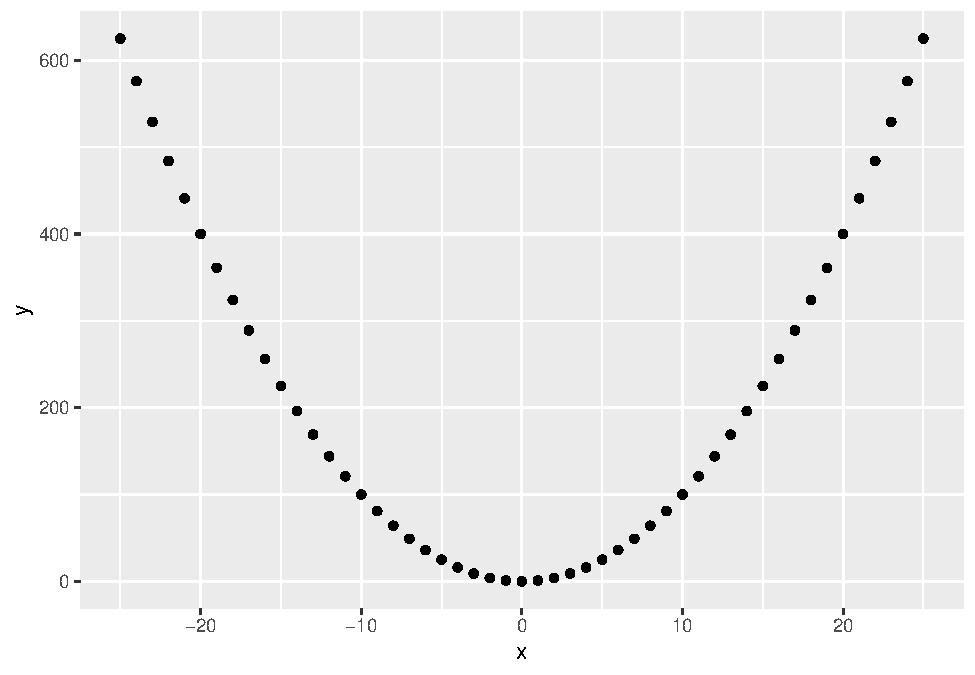
\includegraphics{_main_files/figure-latex/non_linear-1.pdf}

The relationship is clearly not linear. But we can still fit a regression and get a result:

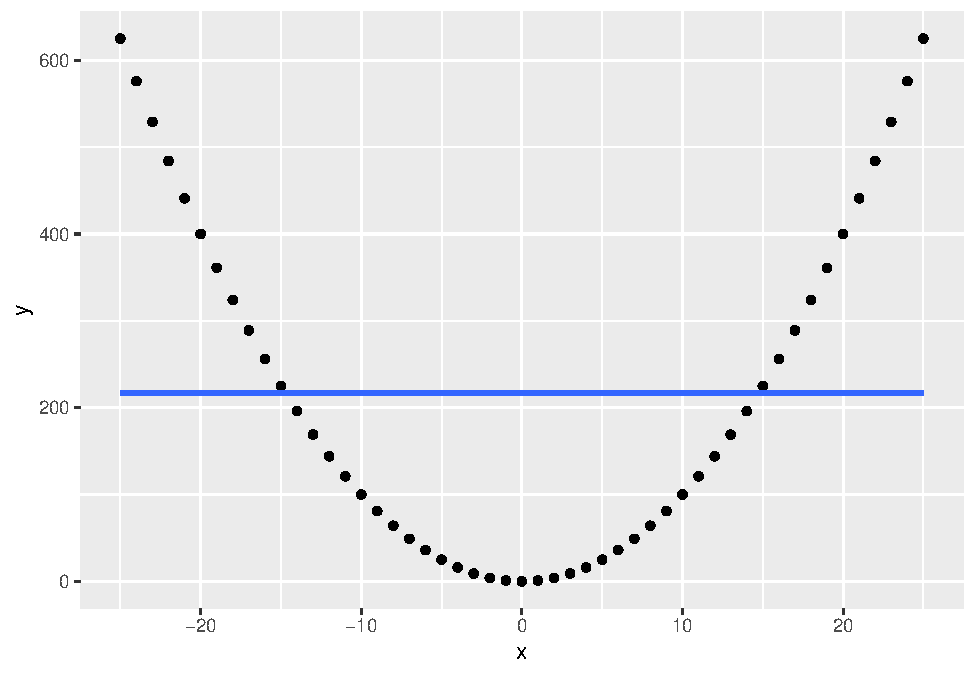
\includegraphics{_main_files/figure-latex/non_linear_reg-1.pdf}

The regression line shows us that \texttt{x} and \texttt{y} are completely uncorrelated. This is clearly not true, but as our linear regression assumes linearity, it tries to model the relationship in linear terms.

What we can do in such cases is to transform the variable in question in a non-linear way. Here the quadratic relationship is easy to spot, so if we transform \(x\) to \(x^2\), this happens:

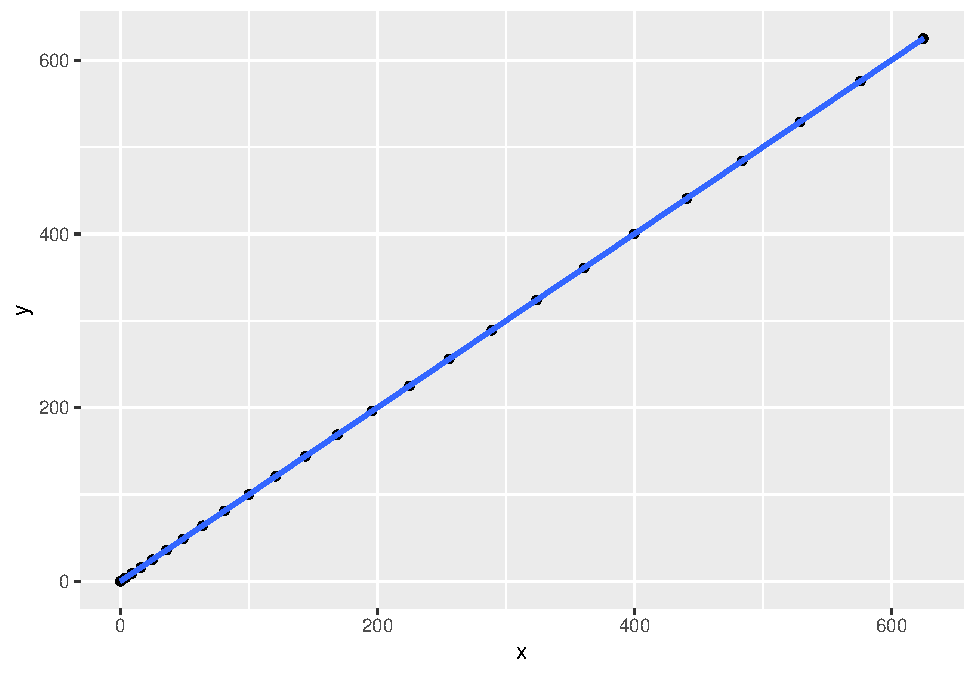
\includegraphics{_main_files/figure-latex/non_linear_reg_squared-1.pdf}

The non-linear relationship between \texttt{x} and \texttt{y} has been transformed into a linear one.

For real world data, the non-linearity most often is not as straightforward to spot as in this example. A first step to approach this, is inspecting a scatterplot matrix. This is usually done before starting to model to identify relationships between the variables used.

\begin{verbatim}
## Warning: package 'GGally' was built under R version 4.2.3
\end{verbatim}

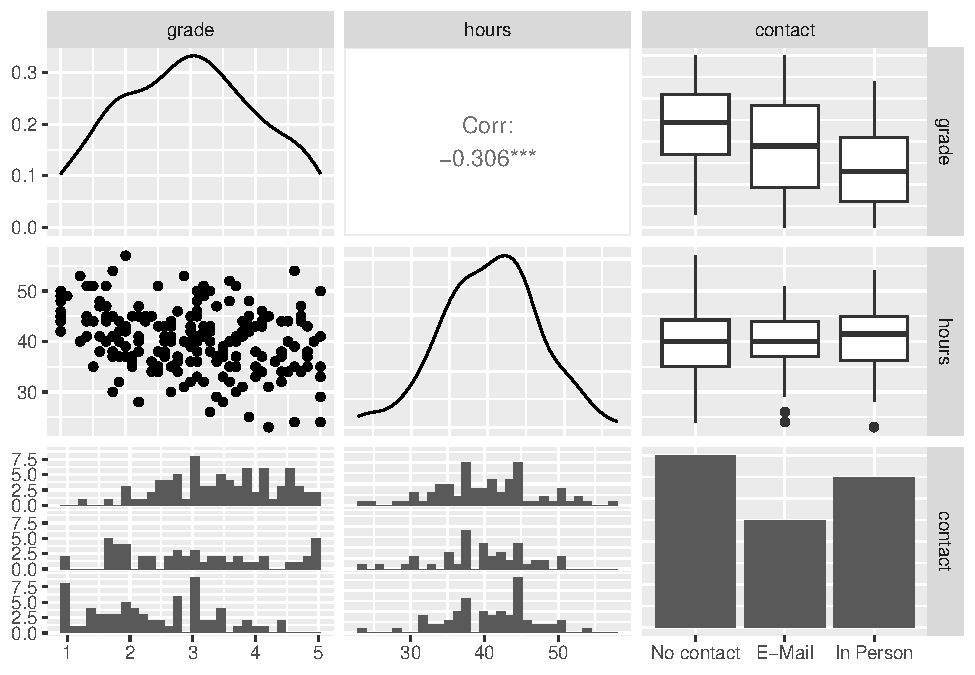
\includegraphics{_main_files/figure-latex/scatterplot_matrix-1.pdf}

The diagonal displays the distribution of all variables included. Here metric variables are displayed as density plots and categorical variables as bar plots. Below and above the diagonal the relationship between two variables is shown. The scatterplot on the left of the second row is the one between \texttt{hours} and \texttt{grade} we have already seen several times. There is no indication of non-linearity here. What we have not inspected yet, is the relationship between \texttt{contact} and the two other variables.

The bottom row contains histograms of the two metric variables by the category of contact, the right column boxplots for the same combination. Without going into too much detail on both types of plots, both show us how the distribution for both metric variables changes by category. The more personal the contact with the lecturer, the lower the center of the distribution of final grades is. This makes sense, as we have already seen this correlation in the results of our model. Between \texttt{hours} and \texttt{contact} there seems to be no correlation. The amount of hours a student invests in writing the paper, does not lower the hours invested in a systematic way.

But this does not clear the model of suspicions of non-linearity just yet. Even when all pairwise relationships are linear, controlling for multiple variables at the same time can introduce non-linearity for this specific combination. One way to approach this is to inspect the \emph{Residuals vs.~Fitted} plot. As the name suggests, this plots the fitted values, i.e.~the estimates for our dependent variables based on the model, against the residuals of the dependent variable. When the relationship is linear, we should see a more or less straight line along the x-axis, where \(y = 0\).

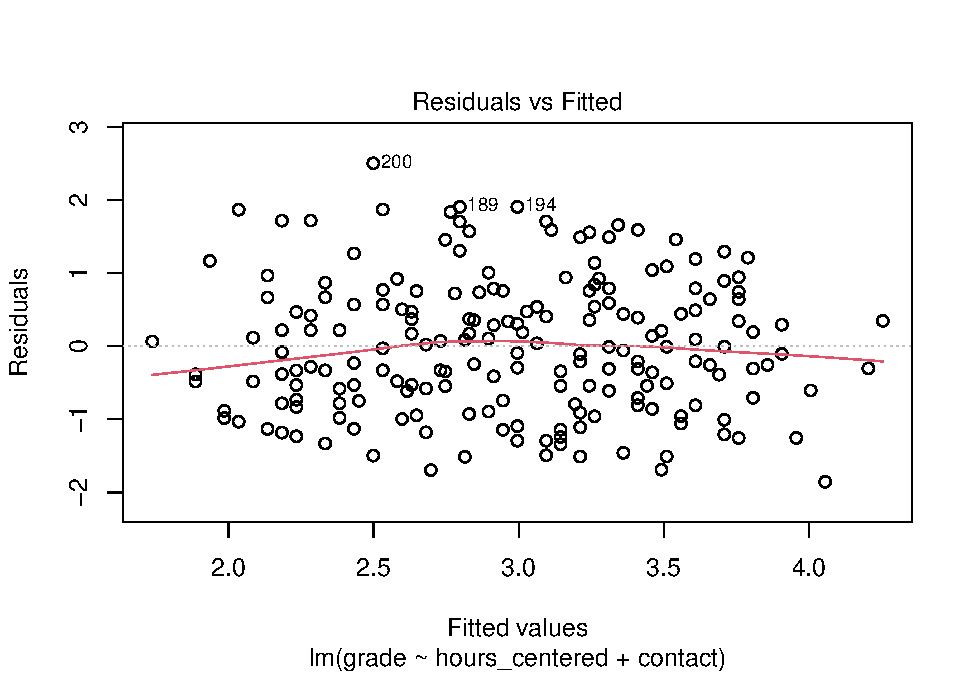
\includegraphics{_main_files/figure-latex/residuals_fitted-1.pdf}

For many use cases, the line is straight enough, indicating no clear and strong patterns of non-linearity. Still the residuals seem to be slightly off for very good and very bad estimated grades.

Besides violating the assumption of linearity, patterns in the residuals vs.~fitted plot can also indicate that there is some important explanatory variable missing from the model. We will return to this after we have applied the further tests and discussed the remaining assumptions.

\hypertarget{normally-distributed-residuals}{%
\subsection{Normally distributed residuals}\label{normally-distributed-residuals}}

Another assumptions in linear regression is that the residuals are normally distributed. This is especially relevant for a sample with a small \(n\) as the test statistics tend to get unreliable in these cases if the residuals are not normally distributed. For larger samples, as in our case, this is not as problematic. Still, systematic deviations from normality can indicate that the model is not \emph{parsimonious}. This means that either not all relevant variables are included or that variables are included that are not necessary for the model.

We get a first idea of the distribution from the model summary. This shows us the median as well as the 25- \& 75-percentiles and the minimum and maximum values. While strong and clear violations against the normality assumption could already be visible here, these measures are not enough to actually test for normality. A more informative and accurate approach is using a \emph{Q-Q plot}. This plots the standardizes residuals, the residuals divided by their standard error, against a theoretical normal distribution. If the residuals are perfectly normally distributed, each data point lies on the diagonal, if they are not they move away from the line. Small deviations, especially in the tails, should not be over emphasized. What we are looking for are clear and systematic deviations.

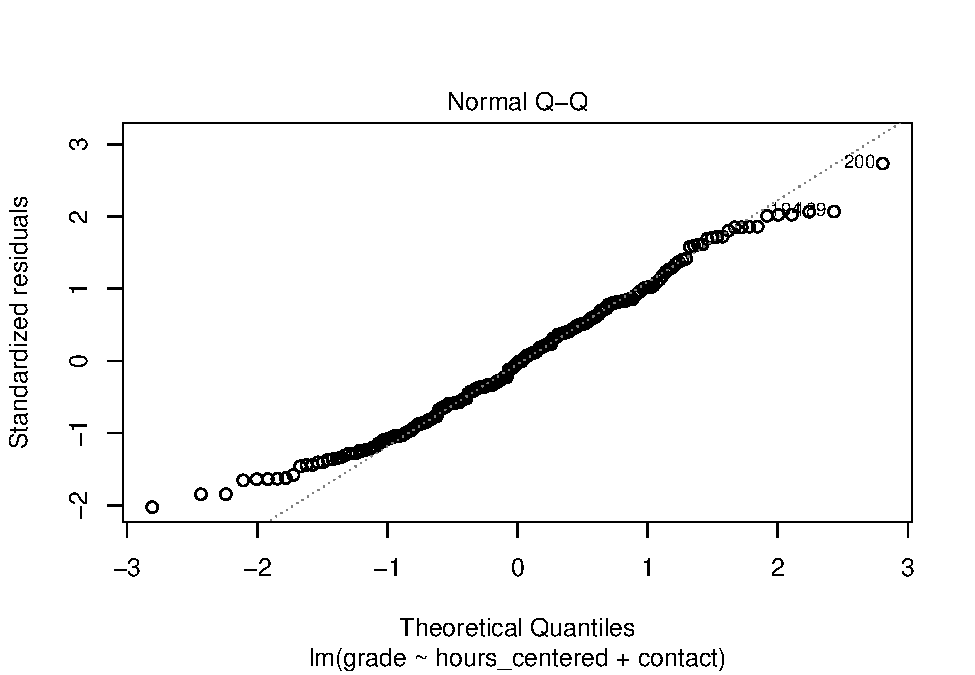
\includegraphics{_main_files/figure-latex/qq-1.pdf}

In the case of our model, most data points lie on the diagonal, while there are some small deviations in the tails. As our n is large enough, this should not be problematic. It may indicate that the model is not perfectly parsimonious but there is no clear cause for concern here.

\hypertarget{homoscedasticity}{%
\subsection{Homoscedasticity}\label{homoscedasticity}}

The \emph{homoscedasticity} assumption states that the residuals are expected to have a constant variance over the whole range of the dependent variable. Let us assume that the variance of our residuals would be lower for very good grades and higher for very bad ones. This would indicate that we can make more accurate estimates for better grades than for worse ones as a small variance would indicate smaller residuals and thus a smaller error. For the assumption to hold we must be able to make about the same quality of estimates, be it high or low, for all values of \texttt{grade}.

The problem is that the computation of the standard errors, test statistics and p-values depends on this assumption. If the assumption is violated, if we have \emph{heteroscedasticity}, these measures are not reliable anymore.

The problem often occurs when the dependent variable is not symmetric. In the scatterplot matrix above, we already saw that \texttt{grade} is fairly symmetrically distributed, so we would not expect problems here. If our dependent variable was asymmetrical, transforming it to be more symmetrical, e.g.~by using the logarithm or a square root, could help.

To check for problems with heteroscedasticity, we can use the \emph{Scale-Location} plot. This plots the fitted values against the square root of the standardized residuals. For homoscedasticity to hold, we should see our data points as a horizontal band with more or less constant width running from the left to the right. The same goes for the plotted line.

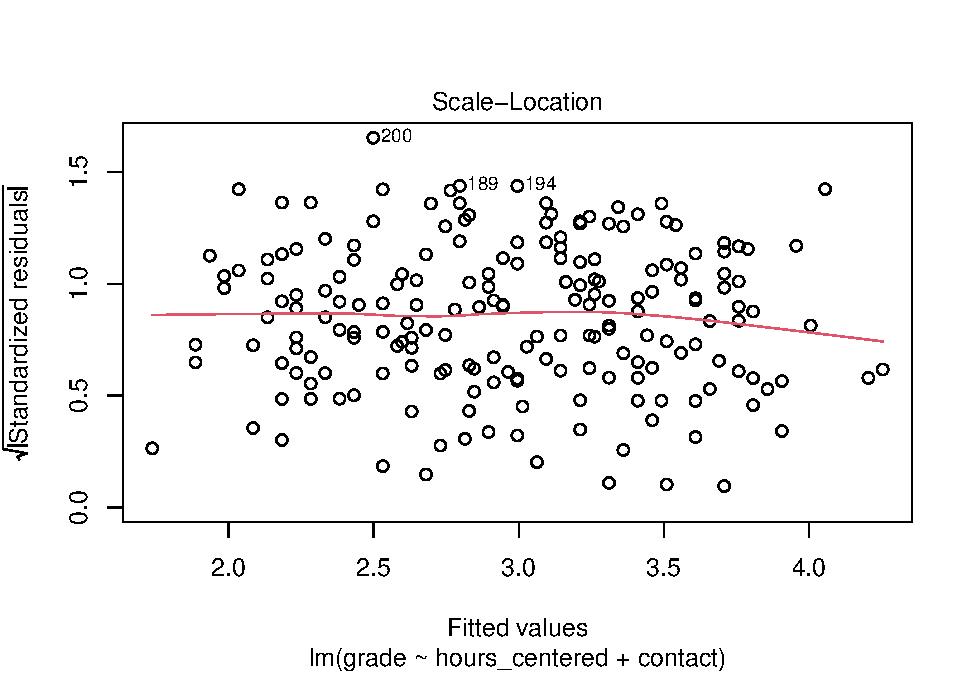
\includegraphics{_main_files/figure-latex/homoscedasticity-1.pdf}

In our case the homoscedasticity assumption holds. Slight variations are not problematic and overall the variance is constant.

\hypertarget{no-overly-influential-data-points}{%
\subsection{No overly influential data points}\label{no-overly-influential-data-points}}

Observations can get highly influential if they have unusual values. Sometimes these are extremely low or high values on some variable. But even ``normal'' values on two or more variables can get unusual in their combination. Imagine a student with \(60\) invested hours. A high value but not overly extreme. Now the same student had in person contact with their lecturer but still received a \(5.0\). This could potentially be an influential data point as this combination is unusual in terms of what the model expects. In case of our model this observation would most probably not be overly influential. But imagine the same observation with \(300\) invested hours. Such extreme cases can influence the fit by figuratively ``pulling'' the regression line in their direction.

We can divide influential data points into unusual values on the dependent variable, \emph{outliers}, and unusual values on independent variables, \emph{high leverage points}. The latter have high leverage because they ``pull'' on the regression lines and thus change the slope. As a rule of thumb, we can consider values with standardized residuals over \(3\) or under \(-3\) outliers. Concerning the dependent variables we can compute the \emph{leverage statistic}. Here values that exceed \(2 * (p + 1) / n\), where \(p\) is the number of predictors, are considered as having high leverage. We can inspect both at the same time in the \emph{Residuals vs.~Leverage} plot.

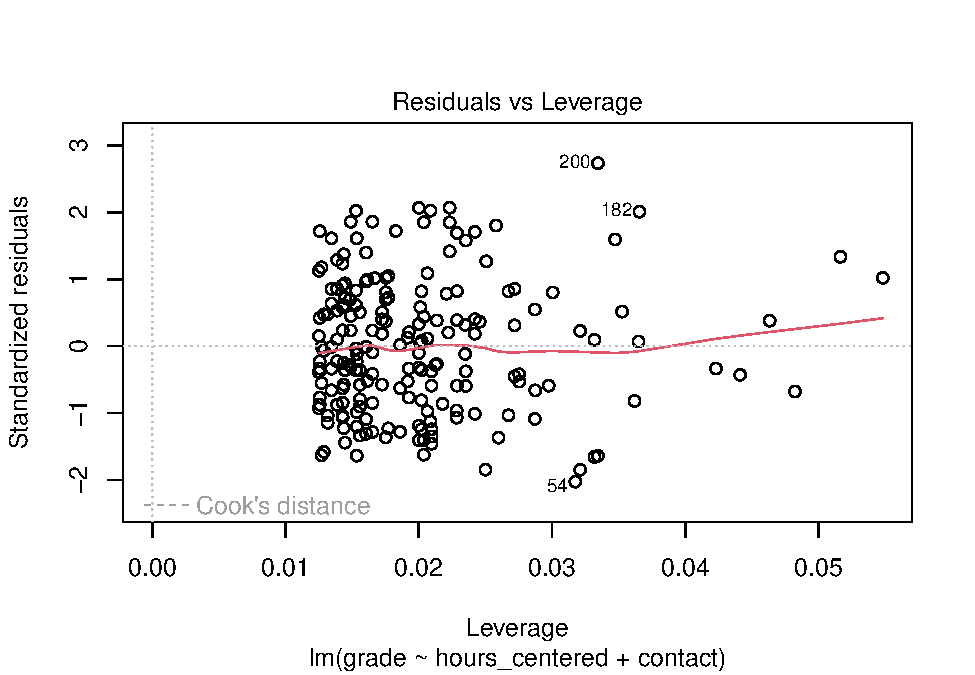
\includegraphics{_main_files/figure-latex/residuals_leverage-1.pdf}

We can see that there are no clear outliers. To assess points with high leverage we first have to compute the threshold as: \(2 * (3 + 1) / 200 = 0.04\). Note that while we have two independent variables in our model, we actually have three predictors due to our categorical variable. Thus we have to compute with \(p = 3\) instead of \(p = 2\). We can see that there are a number of points that exceed this value. The question is, why do these values exist? Sometimes these are measurement errors, extreme values or unusual combinations that come down to the researcher recording the wrong values into the data set. In these cases we can try to fix the errors or remove the observations from the data. As we have several values with high leverage, this seems highly unlikely. But if we had not simulated the data ourselves and knew that there is no error, we should at least check. What seems more probable though, and is often the actual root of high leverage, is that there are variables missing from the model that could explain the high values. In this case the values should be lower after we include the missing variables into the model. We will return to this later.

We also may not have a serious problem here. Leverage on its own does not have to be problematic. Some data points will always be more influential than others and remember that the cutoff is always just a rule of thumb. As said above, it is the combination of unusual values that tends to get problematic. We can check for observations that are outliers and have high leverage visually in our plot. Problematic observations tend to gather in the upper and lower right corners. As neither are populated for our model, we can not really conclude that we have overly influential data points.

\hypertarget{no-multicollinearity}{%
\subsection{No (multi)collinearity}\label{no-multicollinearity}}

The final assumption we will discuss here, is the absence of (high) collinearity between the predictor variables. \emph{Collinearity} is present, if two independent variables are highly correlated with each other. This can become a problem as it gets harder to individually estimate the effects for both variables on the outcome as the collinear variables vary together at the same time.

Often collinearity can already be spotted in the correlation matrix. Considering our matrix above we saw no clear indication that \texttt{hours} and \texttt{contact} are correlated. But the problem can get more complicated if we include three or more independent variables in our model. While none of the pairs of variables may be highly correlated, correlation may exist for a set of three or more of those variables. In these cases we speak of \emph{multicollinearity}. We can not spot this in a correlation matrix, but there is an easy to use measure available.

The \emph{variance inflation factor} (VIF) can be used to inspect (multi)collinearity between two or more independent variables accurately. A VIF of \(1\) would indicate no collinearity. For real world data this is almost never true as some amount of collinearity always exists. But in general we can say that the VIF should be near \(1\) and should not exceed a value of \(5\).

Let us compute the measure for our model with \texttt{hours\_centered} and \texttt{contact}:

\begin{verbatim}
## Warning: package 'car' was built under R version 4.2.3
\end{verbatim}

\begin{verbatim}
## hours_centered        contact 
##       1.004352       1.004352
\end{verbatim}

Both values are very close to \(1\) so we can conclude that we did not violate the assumption. But what could we do, if we did? One approach is to just delete one of the highly correlated independent variables from the model. As they vary together, it may be save to exclude one of them without losing to much information. Another approach would be to combine both variables into a new measure. Let us imagine that besides \texttt{contact} we would have another variable in our model, measuring how well a student feels supported by their lecturer in writing the paper. We could also imagine both variables being strongly correlated as they measure comparable concepts. We could then either drop one of the variables, maybe losing some information in the process, or we could combine both into a new variable which measures the form and the feeling of support at the same time, maybe leading to a more accurate estimate while at the same time eliminating the problem of collinearity. Which one is the right solution depends on the specific case.

\hypertarget{returning-to-our-research-question-1}{%
\section{Returning to our research question}\label{returning-to-our-research-question-1}}

When we tested for linearity above, we saw a mild pattern in the data which is not explainable by a violation of the assumption of linearity and thus could be an indication of a missing relevant explanatory variable in our model. Some of the other tests also supported this notion. The Q-Q plot showed us that the residuals have some slight deviations from normality in the tails. While these deviations are small enough to not cause concern on their own, taken together with the residuals vs.~fitted plot this gives more weight to the suspicion that some important variable is missing. We also identified some observations with high leverage. While we can rule out errors in our data, the high leverage could also be explainable by a missing variable.

But which variable could be missing from the model? If our DAG is correct, we can rule out \texttt{attendance} and \texttt{previous\_grades}. We did assume that \texttt{contact} is a confounder for \texttt{hours} and \texttt{grade} and thus included it in our model. Of course we could also miss a variable that is not in our data at all, or even one that is not measureable. As we did simulate the data, we know this is not true, but with real world data this is always a possibility.

Let us think about the \texttt{contact}variable once more. We did assume, that the more personal the contact, the more efficiently the time working on the paper can be used. And here may lie the problem. The way we included \texttt{contact} in the model is not the way we reasoned in our DAG. It would be correct if we assumed that the more personal the contact, the less time is invested. But we already saw in the scatterplot matrix that there is no such relationship between the variables. To specify the effect of \texttt{contact} in the model correctly, reflecting the idea of a more efficient use of time the closer the contact was, we have to include it as an interaction with \texttt{hours}.

\hypertarget{interactions}{%
\subsection{Interactions}\label{interactions}}

In an \emph{interaction}, we assume that the effect of one variable differs based on the value of another variable. Let us return to the formula for a multiple regression with two variables:

\[y = \beta_0 + \beta_1*x_1 + \beta_2*x_2 + \epsilon\]

Here we assume that the value of \(y\) varies with the value of \(x_1\) and \(x_2\) as indicated by the coefficients \(\beta_1\) and \(\beta_2\).

But we could also follow the notion that the value of \(x_1\) influences \(y\) differently based on the value of \(x_2\). For example the effect of \(x_1\) on \(y\) could be higher when \(x_2\) also has a high value. This is an interaction and is reflected in the formula by adding an additional multiplicative term between the two dependent variables with an additional associated coefficient:

\[y = \beta_0 + \beta_1*x_1 + \beta_2*x_2 + \beta_3 * x_1 * x_2 + \epsilon\]

To get a better understanding of this, let us return to our model and add an interaction between \texttt{hours\_centered} and \texttt{contact}.

\begin{verbatim}
## 
## Call:
## lm(formula = grade ~ hours_centered + contact + hours_centered * 
##     contact, data = grades)
## 
## Residuals:
##      Min       1Q   Median       3Q      Max 
## -1.77816 -0.72882 -0.08719  0.56140  2.53271 
## 
## Coefficients:
##                                 Estimate Std. Error t value Pr(>|t|)    
## (Intercept)                      3.44466    0.10345  33.298  < 2e-16 ***
## hours_centered                  -0.02893    0.01535  -1.885  0.06098 .  
## contactE-Mail                   -0.46775    0.16729  -2.796  0.00569 ** 
## contactIn Person                -1.01493    0.15171  -6.690 2.33e-10 ***
## hours_centered:contactE-Mail    -0.02377    0.02657  -0.895  0.37204    
## hours_centered:contactIn Person -0.05017    0.02442  -2.055  0.04125 *  
## ---
## Signif. codes:  0 '***' 0.001 '**' 0.01 '*' 0.05 '.' 0.1 ' ' 1
## 
## Residual standard error: 0.9253 on 194 degrees of freedom
## Multiple R-squared:   0.28,  Adjusted R-squared:  0.2615 
## F-statistic: 15.09 on 5 and 194 DF,  p-value: 1.63e-12
\end{verbatim}

How can we interpret these results? While the estimates for the intercept and for having e-mail or personal contact in comparison to having no contact at all have barely changed, the coefficient for the amount of hours invested substantially shrunk to almost half its former value. Until now we assumed that the effect of \texttt{hours} would be the same for each student. Now that we have included an interaction we assume that the effect of \texttt{hours} differs, based on the form of contact a student had.

Let us rewrite our formula for \(\hat{y}\) including the interaction. As we are interacting with a categorical variable with three categories, we have to add two interaction terms. The first for the effect of invested hours when e-mail contact was made and the second for the effect of hours when contact was made in person, in both cases compared to having had no contact.

\[\hat{y} = b_0 + b_{hours\_centered} * x_{hours\_centered} +\\
b_{E-Mail} * x_{E-Mail} + b_{In Person} * x_{In Person} +\\
b_{hours\_E-Mail} * x_{hours\_centered} * x_{E-Mail} +\\
b_{hours\_{In Person}} * x_{hours\_centered} * x_{In Person}\]

Let us now also add the coefficients from the model:

\[\hat{y} = 3.44466 -0.02893 * x_{hours\_centered} -\\
0.46775 * x_{E-Mail} -1.01493 * x_{In Person} -\\
0.02377 * x_{hours\_centered} * x_{E-Mail} -\\
0.05017 * x_{hours\_centered} * x_{In Person}\]

We can now consider the three possible forms of contact one by one.

What happens, when a student had no contact? To explore this, we return to the regression formula and equal \(x_{E-Mail}\) and \(x_{In Person}\) to \(0\), which means that no contact was made beforehand. Note that for now we do not care about the actual value of \texttt{hours\_centered}.

\[\hat{y} = 3.44466 -0.02893 *x_{hours\_centered} -\\
0.46775 * 0 -1.01493 * 0 -\\
0.02377 * x_{hours\_centered} * 0 -\\
0.05017 * x_{hours\_centered} * 0\]

This shortens to:

\[\hat{y} = 3.44466 -0.02893 *x_{hours\_centered}\]

For a student who did not make contact, we would estimate the final grade as the intercept minus \(0.02893\) per hour invested more than the mean of \texttt{hours\_centered}. Having equaled \(x_{E-Mail}\) and \(x_{In Person}\) to \(0\) not only ``switched off'' the effects of \texttt{contact} but also removed the interaction effects from the equation, the estimated effect for \texttt{hours\_centered} is only its coefficient of \(-0.02893\).

What happens, when a student had e-mail contact?

\[\hat{y} = 3.44466 -0.02893 * x_{hours\_centered} -\\
0.46775 * 1 -1.01493 * 0 -\\
0.02377 * x_{hours\_centered} * 1 -\\
0.05017 * x_{hours\_centered} * 0\]

This shortens to:

\[\hat{y} = 3.44466 -0.02893 *x_{hours\_centered} -\\
0.46775 -\\
0.02377 * x_{hours\_centered}\]

and further to:

\[\hat{y} = 2.97691 -0.0527 *x_{hours\_centered}\]

The intercept is reduced by the coefficient of having e-mail contact, but what is actually of interest here is the effect that \texttt{hours\_centerd} has. For a student who had e-mail contact, each hour invested above the mean reduces the estimated grade by \(-0.0527\).

We can compute the same for a student with personal contact:

\[\hat{y} = 3.44466 -0.02893 * x_{hours\_centered} -\\
0.46775 * 0 - 1.01493 * 1  -\\
0.02377 * x_{hours\_centered} * 0 -\\
0.05017 * x_{hours\_centered} * 1\]

\[\hat{y} = 3.44466 -0.02893 *x_{hours\_centered} -\\
1.01493 -\\
0.05017 * x_{hours\_centered}\]

\[\hat{y} = 2.42973 -0.0791 *x_{hours\_centered}\]

For a student who had in person contact, each hour invested above the mean reduces the estimated grade by \(-0.0791\).

In practice we would have reached these conclusions more quickly by inspecting the output from our model and just subtracting the corresponding interaction effect from the effect for \texttt{hours\_centered}, but it is important to understand what happens in the formula to get a full grasp on linear regression models.

In the model without the added interaction we concluded that on average each hour invested above the mean decreases the final grade by about \(-0.5\). Now we see that the effect of hours depends on the form of contact had. This reflects the theoretical assumption from our DAG that time can be used more efficiently the more personal the form of contact was.

The same DAG that informed our best model from last week now lead us to including the interaction. This underlines the importance of thorough theoretical thinking before starting to model. It was not even the case that the DAG was wrong, but our conclusions we drew from it were at least not completely right. If we had invested more time, we could have build the correct model directly. In our case we first needed the regression diagnostics to tell us that something might be off before we figured out our error.

\hypertarget{regression-diagnostics-revisited}{%
\subsection{Regression diagnostics (revisited)}\label{regression-diagnostics-revisited}}

We now have a theoretically sound model, but did we also solve the problems indicated in the regression diagnostics?

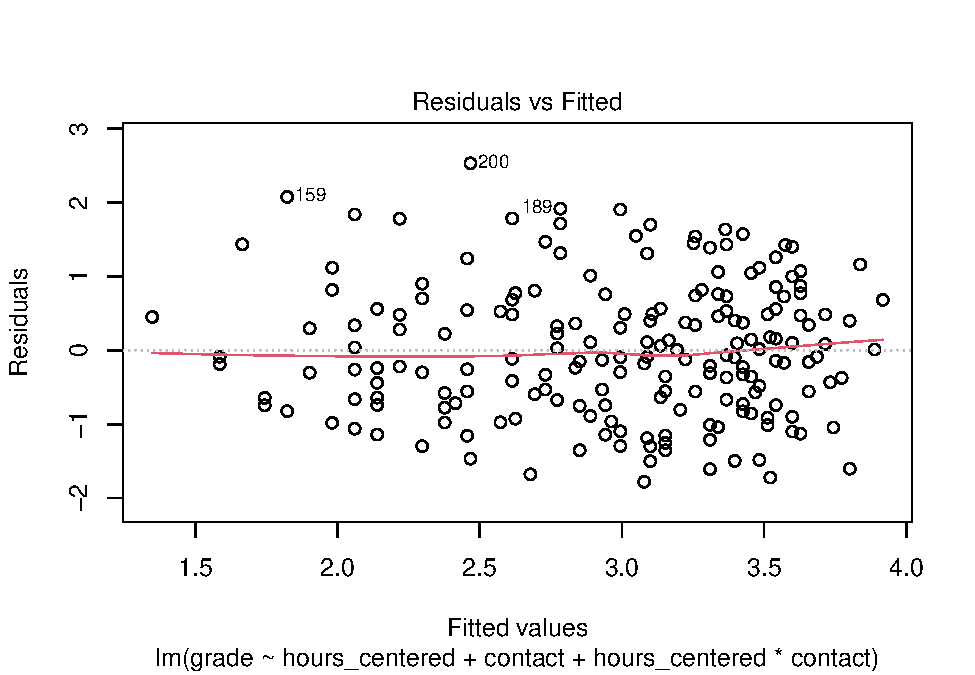
\includegraphics{_main_files/figure-latex/residuals_fitted_revisit-1.pdf}

The residuals vs.~fitted plot now shows an almost straight horizontal line with no clear visible patterns. This indicates that the problem we saw with our former model actually came down to a missing variable, or to be more precise a missing term in our case.

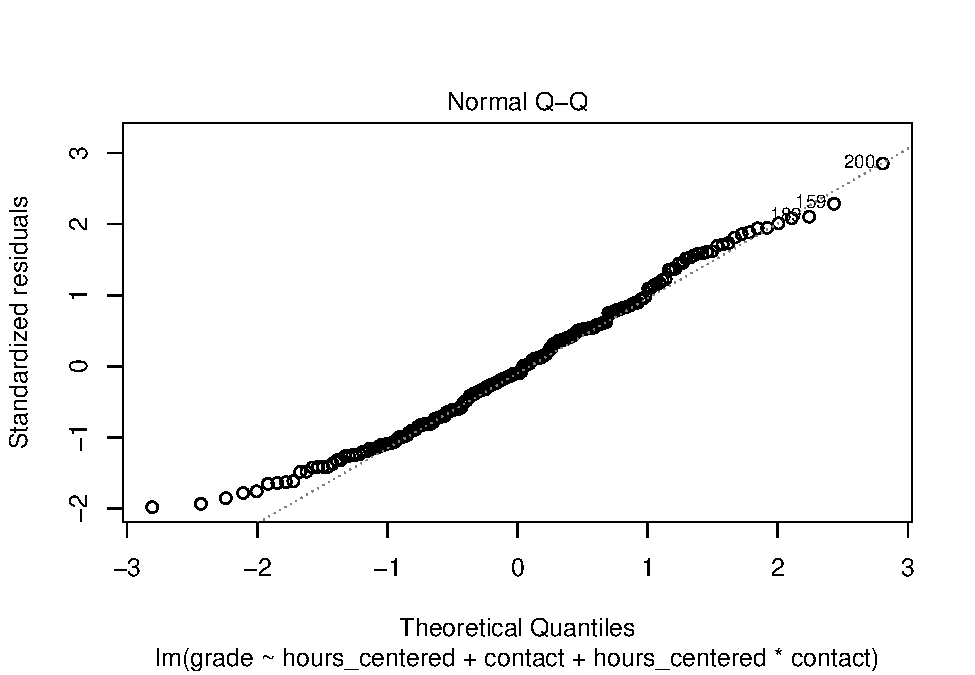
\includegraphics{_main_files/figure-latex/qq_revisited-1.pdf}

The Q-Q plot now also shows more normally distributed residuals. While there are still some small deviations at the lower tail these do not indicate a remaining severe problem. The deviations are smaller than before and also not drastic in absolute terms. Also, as stated above, violating the normality assumption is less problematic with a high \(n\) and few variables in the model, which is still true for our case.

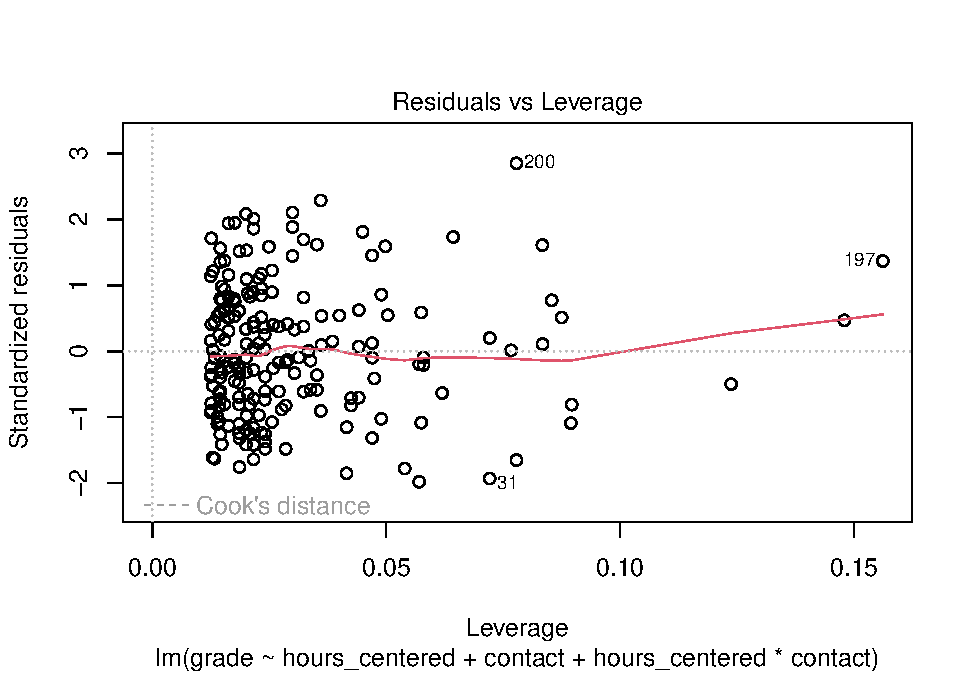
\includegraphics{_main_files/figure-latex/residuals_leverage_revisited-1.pdf}

Adding the interaction term actually increased the leverage of the more influential observations. When we recompute the threshold as \(2 * (5 + 1) / 200 = 0.06\), we see that there still some observations with values higher than this. What has not changed, is that there are no clusters of observations in the lower or upper right corners. Overall we can conclude, that this problem is present but negligible. When there are observations that are problematic on both values at the same time, these also get marked by a red dashed line in the plot. This is also not present.

\hypertarget{conclusion}{%
\section{Conclusion}\label{conclusion}}

Over the last three sessions we have learned what a linear regression is, how its formula works, how to interpret the results for different kinds of variables as well as how to check and correct violations of its underlying assumptions.

At the same time we built a model, which in its final version is able to accurately estimate our effect of interest. But we had one immeasurable advantage: We simulated the data ourselves and thus knew where the journey was going to end up from the start. We knew our DAG was correct because the data was simulated in this way and we also knew that there was going to be a interaction effect to solve the remaining diagnostic problems. Sneaky, right? But in real world data, we do not have these advantages. Our DAGs can be incorrect and we may or may not find the missing part of the puzzle that elevates an OK model to a great one. All we can do is think, explore our data, think again, run diagnostics, think again and maybe most importantly do not give up along the way.

In the \protect\hyperlink{lin-a}{next session} we will return to our NBA data and try to apply everything that we have learned over the last sessions.

\hypertarget{resources-1}{%
\section{Resources}\label{resources-1}}

Most textbooks on statistics include introductions and discussion on using linear regressions. The following resources were the ones actually used in writing the last three sessions:

The textbook from Kohler and Kreuter gives a thorough introduction to linear regression and other statistical concepts. While all code examples are written in Stata, the underlying statistics are the same, no matter the coding language. The book is also available in English.

Kohler, Ulrich \& Frauke Kreuter (2017). Datenanalyse mit Stata. Allgemeine Konzepte der Datenanalyse und ihre praktische Anwendung. 5. aktualisierte Auflage. Berlin, Boston: De Gruyter Oldenbourg.

\hfill\break

James, Gareth; Daniela Witten; Trevor Hastie \& Robert Tibshirani (2021). An Introduction to Statistical Learning. with Applications in R. Second Edition. New York: Springer.

\hfill\break

Manderscheid, Katharina (2017). Sozialwissenschaftliche Datenanalyse mit R. Eine Einführung. 2. Auflage.Wiesbaden: Springer VS.

\hypertarget{lin-a}{%
\chapter{Linear Regression - Application}\label{lin-a}}

After we have learned the ins and outs of linear regression we will now
return to our NBA data. We already saw, that there was an interesting
relationship between the points a player makes per game and the salary
he receives in \protect\hyperlink{eda-1}{session 2}. In \protect\hyperlink{dags-1}{session 4} we also
built a DAG that reflects our assumptions about the data generating
process. Based on the DAGs implications we can now build a linear
regression model and try to estimate the effect of interest as
accurately as possible.

\hypertarget{objectives-5}{%
\section{Objectives}\label{objectives-5}}

\begin{itemize}
\tightlist
\item
  Estimate the effect of interest, scored point on salary, using a
  linear regression
\item
  Applying diagnostics to the model and correct mistakes
\item
  Interpret the final model
\end{itemize}

\hypertarget{r-functions-covered-this-week-1}{%
\section{R functions covered this week}\label{r-functions-covered-this-week-1}}

\begin{itemize}
\tightlist
\item
  \texttt{lm()} : Fits a linear regression model. It takes a regression
  formula and the data to be modelled on. It returns a model object
  that is used by the functions below.
\item
  Displaying regression results

  \begin{itemize}
  \tightlist
  \item
    \texttt{summary()} : Base R function for summaries on different kinds
    of objects. Used on a linear regression model object,
    information on the coefficients and associated measures, the
    model fit as well as on the distribution of residuals is
    returned.
  \item
    \texttt{tidy()} \& \texttt{glance()}: Functions from \textbf{broom} package. They
    return model information as tibbles. The former returns the
    coefficients and associated measures, the latter the model fit.
  \end{itemize}
\item
  Regression diagnostics

  \begin{itemize}
  \tightlist
  \item
    \texttt{plot()} : Base R function for plotting. Used an a model object,
    plots used in regression diagnostics are returned.
  \item
    \texttt{autoplot()} : From the \textbf{ggfortify} package. Returns the same
    plots on regression diagonstics, but in the style of
    \textbf{ggplot2}.
  \item
    \texttt{vif()} : From the \textbf{car} package. Used on a model object, it
    returns the variance inflation factors (VIF) used in regression
    diagnostics.
  \end{itemize}
\item
  \texttt{log()} \& \texttt{exp()}: Base R functions. The former computes the
  \emph{logarithmus naturalis} of a variable, the latter the exponential
  function. Both can be used in transforming skewed variables or in
  reversing each others transformations.
\item
  \texttt{I()} : Base R function. Used in a regression formula it indicates
  that an expression should be evaluated as is, instead of in the
  formula syntax. Can for example be used to square a variable in a
  regression formula.
\end{itemize}

\hypertarget{research-question}{%
\section{Research question}\label{research-question}}

Picking up from session 2 \& 4, our research question is still to get an
unbiased estimate for the effect from points scored on the salary a NBA
player receives. We already constructed a DAG that reflects our
assumptions for the underlying data generating process. Let us revisit
this briefly:

\includegraphics{_main_files/figure-latex/dag_final-1.pdf}

The implications of our DAG were that we only have to control for the
position a player occupies to get an unbiased estimate for our effect of
interest. The path that passes the body height is already closed by
controlling for position and the team a player plays for as well as the
season an observation was recorded in do not lie on an paths from our
main independent to our dependent variable. Based on this we construct
our model.

Now let us get to it and load the NBA data we prepared in week 2.

\begin{Shaded}
\begin{Highlighting}[]
\FunctionTok{library}\NormalTok{(tidyverse)}
\FunctionTok{load}\NormalTok{(}\StringTok{"../datasets/nba/data\_nba.RData"}\NormalTok{)}
\end{Highlighting}
\end{Shaded}

\hypertarget{simple-linear-regression-in-r}{%
\section{Simple linear regression in R}\label{simple-linear-regression-in-r}}

To conduct a multiple linear regression in R, we can use the built-in
\emph{base R} function \texttt{lm()}, short for \emph{linear model}. The function is
straightforward to use. As the first argument we write the regression
formula in R's \emph{formula syntax}.

We start building the formula by writing the name of our
\texttt{dependent\_variable} followed by a \emph{tilde} \texttt{\textasciitilde{}}. You can read this as an
\(=\) or as ``regress the dependent variable on''. After the tilde we add
our first \texttt{indepedent\ variable} by again writing out its name. If we
have multiple independent variables in our model - when we are running a
\emph{multiple linear regression} - we can add those by writing a \texttt{+}
followed by the name of the variable to be added.

As an additional argument, the function needs the name of the object
that holds our data.

The goal of our research question is to estimate the effect of the
points per game on the received salary. So to regress \texttt{salary} on
\texttt{career\_PTS}, we just write:

\begin{Shaded}
\begin{Highlighting}[]
\FunctionTok{lm}\NormalTok{(salary }\SpecialCharTok{\textasciitilde{}}\NormalTok{ career\_PTS, }\AttributeTok{data =}\NormalTok{ data\_nba)}
\end{Highlighting}
\end{Shaded}

\begin{verbatim}
## 
## Call:
## lm(formula = salary ~ career_PTS, data = data_nba)
## 
## Coefficients:
## (Intercept)   career_PTS  
##     -851914       552843
\end{verbatim}

This gives us a short output. The first line just echoes our code used
to run the regression. We have seen this in the last session already,
but now we know what the meaning was. After this we have a short block
with the estimated coefficients. As we have run a simple linear
regression, we only get the intercept and the coefficient for the sole
independent variable used in the model. If we would have run a multiple
linear regression, the result would basically look the same, only with
more coefficients to display.

Before we dive into the results, we should talk about how to receive a
more verbose output that does not hide all the other vital information
that is associated with the model.

The easiest way is to use the base R function \texttt{summary()}. This is a
generic R function that returns different summaries, depending on the
object it is used on. We can for example use it on a data frame or
tibble to get some descriptive statistics for the included variables.
For example, we can get information on the distribution of points per
game by writing:

\begin{Shaded}
\begin{Highlighting}[]
\FunctionTok{summary}\NormalTok{(data\_nba}\SpecialCharTok{$}\NormalTok{career\_PTS)}
\end{Highlighting}
\end{Shaded}

\begin{verbatim}
##    Min. 1st Qu.  Median    Mean 3rd Qu.    Max. 
##   0.000   5.100   8.000   8.908  12.000  30.100
\end{verbatim}

When we use \texttt{summary()} on a model object, like the one created by
\texttt{lm()}, we get a different output. Before we apply this we should save
our model in an object. This is good practice in most cases, as we can
now apply all additional analysis of the model on this object and we do
not have to rerun the model every time.

\begin{Shaded}
\begin{Highlighting}[]
\NormalTok{m1 }\OtherTok{\textless{}{-}} \FunctionTok{lm}\NormalTok{(salary }\SpecialCharTok{\textasciitilde{}}\NormalTok{ career\_PTS, }\AttributeTok{data =}\NormalTok{ data\_nba)}
\end{Highlighting}
\end{Shaded}

We can now apply \texttt{summary()} on the object \texttt{m1}, short for ``model 1'':

\begin{Shaded}
\begin{Highlighting}[]
\FunctionTok{summary}\NormalTok{(m1)}
\end{Highlighting}
\end{Shaded}

\begin{verbatim}
## 
## Call:
## lm(formula = salary ~ career_PTS, data = data_nba)
## 
## Residuals:
##       Min        1Q    Median        3Q       Max 
## -14788659  -2023969   -434599   1311807  24326060 
## 
## Coefficients:
##             Estimate Std. Error t value Pr(>|t|)    
## (Intercept)  -851915      76417  -11.15   <2e-16 ***
## career_PTS    552843       7453   74.17   <2e-16 ***
## ---
## Signif. codes:  0 '***' 0.001 '**' 0.01 '*' 0.05 '.' 0.1 ' ' 1
## 
## Residual standard error: 3732000 on 9726 degrees of freedom
## Multiple R-squared:  0.3613, Adjusted R-squared:  0.3612 
## F-statistic:  5502 on 1 and 9726 DF,  p-value: < 2.2e-16
\end{verbatim}

This is the output we saw over the last weeks and it includes an
extended and better readable coefficient block as well as the
information on the residuals and the model fit.

An alternative method of displaying the coefficients in a regular tibble
format is to use \texttt{tidy()} from the \texttt{broom} package.

\begin{Shaded}
\begin{Highlighting}[]
\FunctionTok{library}\NormalTok{(broom)}

\FunctionTok{tidy}\NormalTok{(m1)}
\end{Highlighting}
\end{Shaded}

\begin{verbatim}
## # A tibble: 2 x 5
##   term        estimate std.error statistic  p.value
##   <chr>          <dbl>     <dbl>     <dbl>    <dbl>
## 1 (Intercept) -851914.    76417.     -11.1 1.09e-28
## 2 career_PTS   552843.     7453.      74.2 0
\end{verbatim}

\hypertarget{interpretation}{%
\subsection{Interpretation}\label{interpretation}}

While we know our model is not complete yet, let us still inspect the
results. For each point a player scores per game, his salary rises by
about \(552,000\$\). We see a clear positive and substantial effect. Let
us also inspect the intercept. This tells us that a player who makes no
points per game has to pay the team about \(850,000\). Wait, this does not
make sense\ldots{} To make the intercept more readily interpretable we should
again center our metric dependent variable \texttt{career\_PTS} on its mean.

\begin{Shaded}
\begin{Highlighting}[]
\FunctionTok{mean}\NormalTok{(data\_nba}\SpecialCharTok{$}\NormalTok{career\_PTS)}
\end{Highlighting}
\end{Shaded}

\begin{verbatim}
## [1] 8.907679
\end{verbatim}

\begin{Shaded}
\begin{Highlighting}[]
\NormalTok{data\_nba }\OtherTok{\textless{}{-}}\NormalTok{ data\_nba }\SpecialCharTok{\%\textgreater{}\%} 
  \FunctionTok{mutate}\NormalTok{(}\AttributeTok{PTS\_centered =}\NormalTok{ career\_PTS }\SpecialCharTok{{-}} \FunctionTok{mean}\NormalTok{(career\_PTS))}
\end{Highlighting}
\end{Shaded}

As we have now centered the independent variable of interest on its mean
of \(8.9\) we can rerun the model.

\begin{Shaded}
\begin{Highlighting}[]
\NormalTok{m1 }\OtherTok{\textless{}{-}} \FunctionTok{lm}\NormalTok{(salary }\SpecialCharTok{\textasciitilde{}}\NormalTok{ PTS\_centered, }\AttributeTok{data =}\NormalTok{ data\_nba)}

\FunctionTok{summary}\NormalTok{(m1)}
\end{Highlighting}
\end{Shaded}

\begin{verbatim}
## 
## Call:
## lm(formula = salary ~ PTS_centered, data = data_nba)
## 
## Residuals:
##       Min        1Q    Median        3Q       Max 
## -14788659  -2023969   -434599   1311807  24326060 
## 
## Coefficients:
##              Estimate Std. Error t value Pr(>|t|)    
## (Intercept)   4072633      37840  107.63   <2e-16 ***
## PTS_centered   552843       7453   74.17   <2e-16 ***
## ---
## Signif. codes:  0 '***' 0.001 '**' 0.01 '*' 0.05 '.' 0.1 ' ' 1
## 
## Residual standard error: 3732000 on 9726 degrees of freedom
## Multiple R-squared:  0.3613, Adjusted R-squared:  0.3612 
## F-statistic:  5502 on 1 and 9726 DF,  p-value: < 2.2e-16
\end{verbatim}

The coefficient for points per game has not changed but its
interpretation has. For each point per game over the mean of \(8.9\)
points per game, the salary is estimated to increase by about
\(552,000\$\). At the same time, for each point below the mean the salary
is estimated to decrease by the same amount. The intercept now shows us
the estimated salary of a player who scores \(8.9\) points per game, which
is slightly upwards of \(4,000,000\$\). This makes way more sense.

This model model already achieved a considerable \(R^2\) of \(0.36\). About
\(36\%\) of the variance in salaries is explained by points per game.

Another way to get the model statistics, such as \(r^2\), F-statistic, and
p-value, is to use the \texttt{glance()} function from the broom package. This
function returns a tibble with one row of model summaries.

\begin{Shaded}
\begin{Highlighting}[]
\FunctionTok{glance}\NormalTok{(m1)}
\end{Highlighting}
\end{Shaded}

\begin{verbatim}
## # A tibble: 1 x 12
##   r.squared adj.r.squared    sigma statistic p.value    df  logLik    AIC    BIC
##       <dbl>         <dbl>    <dbl>     <dbl>   <dbl> <dbl>   <dbl>  <dbl>  <dbl>
## 1     0.361         0.361 3732168.     5502.       0     1 -1.61e5 3.22e5 3.22e5
## # i 3 more variables: deviance <dbl>, df.residual <int>, nobs <int>
\end{verbatim}

We can see that the output includes the same information as the summary
of \texttt{m1}, but in a different format. The advantage of using \texttt{glance()} is
that it is easier to manipulate and compare the model statistics using
tidyverse functions. For example, we can use \texttt{bind\_rows()} to combine
the outputs of different models and compare their performance.

\hypertarget{multiple-linear-regression-in-r}{%
\section{Multiple linear regression in R}\label{multiple-linear-regression-in-r}}

The DAG we have constructed above based on our research question
indicated that we also have to include the position a player occupies in
our model. We can add additional independent variables to the formula
used in \texttt{lm()} with a \texttt{+} and the name of the additional variable(s).
This works the same way for all types of variables, i.e.~metric, dummies
or categorical variables. So let us do this now by adding the 5 dummies
we constructed for the positions:

\begin{Shaded}
\begin{Highlighting}[]
\NormalTok{m2 }\OtherTok{\textless{}{-}} \FunctionTok{lm}\NormalTok{(salary }\SpecialCharTok{\textasciitilde{}}\NormalTok{ PTS\_centered }\SpecialCharTok{+}\NormalTok{ position\_center }\SpecialCharTok{+}\NormalTok{ position\_sf }\SpecialCharTok{+}\NormalTok{  position\_pf }\SpecialCharTok{+}\NormalTok{ position\_sg }\SpecialCharTok{+}\NormalTok{ position\_pg, }\AttributeTok{data =}\NormalTok{ data\_nba)}

\FunctionTok{summary}\NormalTok{(m2)}
\end{Highlighting}
\end{Shaded}

\begin{verbatim}
## 
## Call:
## lm(formula = salary ~ PTS_centered + position_center + position_sf + 
##     position_pf + position_sg + position_pg, data = data_nba)
## 
## Residuals:
##       Min        1Q    Median        3Q       Max 
## -14511723  -1950255   -372906   1358768  24433660 
## 
## Coefficients:
##                 Estimate Std. Error t value Pr(>|t|)    
## (Intercept)      3679728     114300  32.193  < 2e-16 ***
## PTS_centered      568019       7474  75.994  < 2e-16 ***
## position_center  1380246     114539  12.050  < 2e-16 ***
## position_sf       125384     102174   1.227 0.219790    
## position_pf       206505      94882   2.176 0.029547 *  
## position_sg      -331033      96841  -3.418 0.000633 ***
## position_pg      -114552     117486  -0.975 0.329572    
## ---
## Signif. codes:  0 '***' 0.001 '**' 0.01 '*' 0.05 '.' 0.1 ' ' 1
## 
## Residual standard error: 3652000 on 9721 degrees of freedom
## Multiple R-squared:  0.3888, Adjusted R-squared:  0.3884 
## F-statistic:  1031 on 6 and 9721 DF,  p-value: < 2.2e-16
\end{verbatim}

\hypertarget{interpretation-1}{%
\subsection{Interpretation}\label{interpretation-1}}

We still see a clear positive effect of points per game on the received
salary after controlling for the position a player occupies. Among those
centers are by far the top earners, making about \(1,400,00\$\) more than
players on other positions. Most other positions show relatively small
effects on the earnings. Power and small forwards earn somewhat more
than other positions on average while point and especially shooting
guards earn less.

We can now compare two fictive cases of a center and a point guard who
each make about \(20\) points per game. What is the estimated salary for
them?

As we have extensively worked with the formulas over the last sessions,
we can now keep it short and calculate the estimate directly. Remember
that we centered the points per game on the mean of about \(8.9\), so
making \(20\) per game would mean scoring about \(11.1\) more compared to
the average player. We will keep it simple here and calculate with \(11\).

\[\hat{y_{center\_20}} = 3679728 + 568019 * 11 + 1380246 = 11,308,183\]

\[\hat{y_{pg\_20}} = 3679728 + 568019 * 11 - 114552 = 9,813,385\]

Despite making the same amount of points per game for their team, the
model estimates that a point guard earns about \(1,500,000\$\) less
compared to a center.

\hypertarget{sidenote-adding-interactions}{%
\subsection{Sidenote: Adding interactions}\label{sidenote-adding-interactions}}

We will not use interactions in this session but we briefly want to
state how we could add them in the formula syntax.

Remember that interactions are multiplicative terms in our regression
formula. Adding them to the R formula syntax works the same way. We add
the new term with a \texttt{+} and use a \texttt{*} between the two variables that we
want to interact.

Here is a non running toy example where we interact two x-variables:

\begin{verbatim}
lm(y ~ x1 + x2 + x1 * x2, data = some_data)
\end{verbatim}

\hypertarget{regression-diagnostics-1}{%
\section{Regression Diagnostics}\label{regression-diagnostics-1}}

So how does our model perform? Did we meet all the regression
assumptions that were introduced last week?

To access the visual tests we used last session, we can just use the
base R function \texttt{plot()}, applied to the model object. If we write
\texttt{plot(m2)}, the console asks us to press \texttt{ENTER} to go through each plot
one by one. We can also add a number as a second argument, specifying
which plot we want to see. For example, \texttt{plot(m2,\ 1)} gives us the
residuals vs.~fitted plot.

But there is an easier way to see all four plots at once. The package
\texttt{ggfortify} expands the functionalities of \texttt{ggplot2} so that we can use
it's \texttt{autoplot()} function to automatically plot all four visual tests
of interest. An added benefit, depending on your taste, is that the
plots are rendered in the style of \texttt{ggplot2}.

\begin{Shaded}
\begin{Highlighting}[]
\FunctionTok{library}\NormalTok{(ggfortify)}

\FunctionTok{autoplot}\NormalTok{(m2)}
\end{Highlighting}
\end{Shaded}

\includegraphics{_main_files/figure-latex/m2_diag-1.pdf}

The residuals vs.~fitted does not show us a more or less straight line
but starts mildly positive, then dips below \(0\) and rises again for
higher estimated salaries. This could indicate at least two thing.
Either we have missed an important independent variable, like in the
last session, or we are actually dealing with some amount on
non-linearity. If it is non-linearity, it is still \emph{mild} non-linearity,
but maybe we should still inspect this.

The Q-Q plot this time shows that the actual residuals are far from
being distributed normally. While we can never expect a perfectly normal
distribution, here the deviations are striking, especially for high
residuals.

The scale-location plot is used to address the assumption of
homoscedasticity. What we want to see, is a straight line with data
points equally distributed around it. This clearly is not the case here.
As it is, the plot indicates that we may be able to estimate small
salaries reasonably well but that the higher the estimate, the more
unreliable our model gets.

The residuals vs.~leverage plot also indicates some problems. There are
some observations that have larger or smaller standardized residuals
compared to the thresholds of \(3\) and \(-3\). The threshold for leverage
is computed as \(2 * (6 + 1) / 9728 = 0.001439145\). We also see some
observations with higher values. While both are rules of thumb and may
not necessarily point to severe problems by themselves, things can get
problematic when there are observations that do not meet the thresholds
for both measures at the same time. This is indicated by clusters in the
lower or upper right corners. This time we can observe this in the lower
right.

We should also test for multicollinearity. We can compute the VIF
measures using a function from the package \texttt{car}.

\begin{Shaded}
\begin{Highlighting}[]
\FunctionTok{library}\NormalTok{(car)}

\FunctionTok{vif}\NormalTok{(m2)}
\end{Highlighting}
\end{Shaded}

\begin{verbatim}
##    PTS_centered position_center     position_sf     position_pf     position_sg 
##        1.050400        2.035722        1.686736        1.512765        1.565004 
##     position_pg 
##        1.916933
\end{verbatim}

The values for any variable should not exceed \(5\) and should be closer
to \(1\). Our value for points shows no signs of multicollinearity. The
values for the position dummies have somewhat higher values, which makes
sense. While there are some players that play multiple positions, for
most a value of \(1\) on one position predicts the other positions as
having a value of \(0\). But as we are still far away from the threshold
of \(5\), there is no need for concern here.

Overall, we have problems! While we do not see signs of problematic
multicollinearity, all other tests indicated clear and in parts severe
problems. We have to put in some more work before we can be confident
that our model accurately estimates the effect of points per game on the
received salary.

Before we start addressing the problems, we should note that the four
plots are highly interactive. It is entirely possible that solving one
of the problems also solves the others or, for added fun, even generates
new ones. This means that we should refrain from turning too many dials
at once and rather change the model one step at a time, see if it
improves things and then address remaining problems in the same way.

\hypertarget{skewed-outcome-variable}{%
\subsection{Skewed outcome variable}\label{skewed-outcome-variable}}

The deviation from normality and the clearly present heteroscedasticity
could both point to the same problem, namely a skewed dependent
variable. Let us examine its distribution first.

\begin{Shaded}
\begin{Highlighting}[]
\NormalTok{data\_nba }\SpecialCharTok{\%\textgreater{}\%} 
  \FunctionTok{ggplot}\NormalTok{(}\FunctionTok{aes}\NormalTok{(}\AttributeTok{x =}\NormalTok{ salary)) }\SpecialCharTok{+}
  \FunctionTok{geom\_density}\NormalTok{()}
\end{Highlighting}
\end{Shaded}

\includegraphics{_main_files/figure-latex/distribution_dv_before-1.pdf}

Our outcome variable is not only skewed, it is \textbf{highly skewed}. While
there are many salaries in the ``lower'' six to seven digits regions, we
also see some extremely high wages up to about \(35,000,000\$\). The
higher the salary the fewer observations we have. That is why we see
such a long flat tail to the right.

This distribution actually is relatively common for income data. In most
surveys of the general population we have many people receiving
relatively low incomes while fewer individuals receive higher or
extremely high incomes. It is still interesting that this also holds
true for a population of high earners such as NBA players. Inequality is
relative. Compared to the general population almost all our players
would be somewhere in the long tail to the right. Compared to their own
population we still see highly substantial differences in outcomes.

We can transform the dependent variable to a different scale to get a
less skewed distribution. A common transformation for income data is to
take the \emph{logarithmus naturalis} of the actual value and then use this
as our dependent variable. To achieve the transformation we can simply
use the base R function \texttt{log()} which as its default computes the \(ln\).

\begin{Shaded}
\begin{Highlighting}[]
\NormalTok{data\_nba }\OtherTok{\textless{}{-}}\NormalTok{ data\_nba }\SpecialCharTok{\%\textgreater{}\%} 
  \FunctionTok{mutate}\NormalTok{(}\AttributeTok{salary\_log =} \FunctionTok{log}\NormalTok{(salary))}

\NormalTok{data\_nba }\SpecialCharTok{\%\textgreater{}\%} 
  \FunctionTok{ggplot}\NormalTok{(}\FunctionTok{aes}\NormalTok{(}\AttributeTok{x =}\NormalTok{ salary\_log)) }\SpecialCharTok{+}
  \FunctionTok{geom\_density}\NormalTok{()}
\end{Highlighting}
\end{Shaded}

\includegraphics{_main_files/figure-latex/transform_dv_log-1.pdf}

While the distribution of the transformed variable also is somewhat
skewed, now to the left, overall it is much more evenly distributed.

We should use the new variable as our outcome an check the tests again.

\begin{Shaded}
\begin{Highlighting}[]
\NormalTok{m3 }\OtherTok{\textless{}{-}} \FunctionTok{lm}\NormalTok{(salary\_log }\SpecialCharTok{\textasciitilde{}}\NormalTok{ PTS\_centered }\SpecialCharTok{+}\NormalTok{ position\_center }\SpecialCharTok{+}\NormalTok{ position\_sf }\SpecialCharTok{+}\NormalTok{  position\_pf }\SpecialCharTok{+}\NormalTok{ position\_sg }\SpecialCharTok{+}\NormalTok{ position\_pg, }\AttributeTok{data =}\NormalTok{ data\_nba)}

\FunctionTok{autoplot}\NormalTok{(m3)}
\end{Highlighting}
\end{Shaded}

\includegraphics{_main_files/figure-latex/m3-1.pdf}

Looking at the scale-location plot first, we can now see a straight line
with our residuals fairly evenly distributed around it. Thus we now
longer see any signs of heteroscedasticity. The Q-Q plot now also
indicates a somewhat more normal distribution of our residuals but there
are substantial deviations still. While high residuals now appear to
more or less follow the normal distribution, small residuals now deviate
stronger than they have before. This reflects the transformation and its
distribution, which now has long tail on the left instead of on the
right, as before. Turning to the residuals vs.~leverage plot we still
see some observations that do not meet the respective thresholds. At the
same time, there appear to be less that simultaneously have high
absolute standardized residuals and high leverage. The residuals vs.
fitted plot now also shows a more even distribution while the signs on
non-linearity remain. We do not have to recompute the VIF measure as we
did not change any independent variables in the model.

\hypertarget{non-linearity}{%
\subsection{Non-linearity}\label{non-linearity}}

Let us now address the non-linearity that is still indicated in the
first plot. We can approach non-linear relationships in our inherently
linear model by adding non-linear transformations of a dependent
variable to the model. But before we start squaring random variables, we
should think about what could be non-linear in our case. We can rule out
our dummy variables for position. This leaves the points scored. The
model already indicates that our suspicion that salary rises with the
points scored could be true. But maybe this relationship is not linear
over its whole range. If you already are among high scorers, scoring one
or two points more than your peers may not be such a substantial
difference and thus may not have the same strong effect on salary.

We should first inspect the relationship between both variables again.
This time we add a LOWESS curve to the plot. This is often helpful in
detecting non-linearity as the curve can change its slope over the range
of the dependent variable. This is also the default for \texttt{geom\_smooth()}.

\begin{Shaded}
\begin{Highlighting}[]
\NormalTok{data\_nba }\SpecialCharTok{\%\textgreater{}\%} 
  \FunctionTok{ggplot}\NormalTok{(}\FunctionTok{aes}\NormalTok{(}\AttributeTok{x =}\NormalTok{ career\_PTS, }\AttributeTok{y =}\NormalTok{ salary)) }\SpecialCharTok{+}
  \FunctionTok{geom\_point}\NormalTok{() }\SpecialCharTok{+}
  \FunctionTok{geom\_smooth}\NormalTok{(}\AttributeTok{se =} \ConstantTok{FALSE}\NormalTok{)}
\end{Highlighting}
\end{Shaded}

\includegraphics{_main_files/figure-latex/non_linearity-1.pdf}

While this is not as clear as we hoped, the line may still indicate some
mild non-linearity as it flattens somewhat for really high point values.
Also we have to keep in mind that the non-linearity may be stronger when
we control for additional variables, as our position dummies.

One common way to address the non-linearity is taking the square of the
dependent variable in question. We should not square our centered points
variable though. Let us inspect what would happen if we squared it.

\begin{Shaded}
\begin{Highlighting}[]
\NormalTok{data\_nba }\SpecialCharTok{\%\textgreater{}\%} 
  \FunctionTok{ggplot}\NormalTok{(}\FunctionTok{aes}\NormalTok{(}\AttributeTok{x =}\NormalTok{ PTS\_centered, }\AttributeTok{y =}\NormalTok{ PTS\_centered }\SpecialCharTok{\^{}} \DecValTok{2}\NormalTok{)) }\SpecialCharTok{+}
  \FunctionTok{geom\_point}\NormalTok{() }\SpecialCharTok{+}
  \FunctionTok{geom\_smooth}\NormalTok{(}\AttributeTok{se =} \ConstantTok{FALSE}\NormalTok{)}
\end{Highlighting}
\end{Shaded}

\includegraphics{_main_files/figure-latex/centered_squared-1.pdf}

As the square of negative values is positive, we would basically
introduce the assumption into the model that there is non-linearity for
low and high scorers and that the effect will be in the same direction.
While our assumption is that there are diminishing returns between being
a high scorer and a \textbf{really} high scorer, we do not assume that making
more points if you are among the lower scorers should have the same
effect. If at all, in these regions additional points could have an even
larger effect.

Because of this we should return to the uncentred version of our
variable. What happens if we square this?

\begin{Shaded}
\begin{Highlighting}[]
\NormalTok{data\_nba }\SpecialCharTok{\%\textgreater{}\%} 
  \FunctionTok{ggplot}\NormalTok{(}\FunctionTok{aes}\NormalTok{(}\AttributeTok{x =}\NormalTok{ career\_PTS, }\AttributeTok{y =}\NormalTok{ career\_PTS }\SpecialCharTok{\^{}} \DecValTok{2}\NormalTok{)) }\SpecialCharTok{+}
  \FunctionTok{geom\_point}\NormalTok{() }\SpecialCharTok{+}
  \FunctionTok{geom\_smooth}\NormalTok{(}\AttributeTok{se =} \ConstantTok{FALSE}\NormalTok{)}
\end{Highlighting}
\end{Shaded}

\includegraphics{_main_files/figure-latex/career_pts_squared-1.pdf}

This is what we wanted, a transformation that expects a stronger
difference the higher the score value is. For the final model we will
thus work with the uncentered variable. We included the centered version
because it is more straightforward to interpret. This is not really a
concern anymore because dreams of easy interpretability have long passed
after transforming two variables.

We could again transform the variable in our data and thus add a second
version, but we can also do so directly in the formula syntax. When we
use the function \texttt{I()} we tell R to interpret anything within the
parentheses as a mathematical expression. This is what we will do below.
Note that we add the point variable as its untransformed and transformed
versions. The first represents the linear parts and the second the
non-linear parts of the effect.

\begin{Shaded}
\begin{Highlighting}[]
\NormalTok{m4 }\OtherTok{\textless{}{-}} \FunctionTok{lm}\NormalTok{(salary\_log }\SpecialCharTok{\textasciitilde{}}\NormalTok{ career\_PTS }\SpecialCharTok{+} \FunctionTok{I}\NormalTok{(career\_PTS}\SpecialCharTok{\^{}}\DecValTok{2}\NormalTok{) }\SpecialCharTok{+}\NormalTok{ position\_center }\SpecialCharTok{+}\NormalTok{ position\_sf }\SpecialCharTok{+}\NormalTok{ position\_pf }\SpecialCharTok{+}\NormalTok{ position\_sg }\SpecialCharTok{+}\NormalTok{ position\_pg, }\AttributeTok{data =}\NormalTok{ data\_nba)}
\end{Highlighting}
\end{Shaded}

We can now reassess the tests for the last model.

\begin{Shaded}
\begin{Highlighting}[]
\FunctionTok{autoplot}\NormalTok{(m4)}
\end{Highlighting}
\end{Shaded}

\includegraphics{_main_files/figure-latex/m4_diag-1.pdf}

The line in the residuals vs.~fitted plot got more straight. It seems
that we actually captured the mild non-linearity that was present before
by adding the squared points value to our model. The scale-location plot
also still indicates no more problems of heteroscedasticity. Contrary,
the data points now are even more evenly distributed compared to \texttt{m3}.
The Q-Q plot has not substantially changed, still showing non-normally
distributed residuals. We can not really fix this now, but we also
learned that this test is less consequential if we have a large \(n\).
Turning to the residuals vs.~leverage plot, we still see several points
that do not meet the thresholds but at the same time we do not see any
points with high values for both. Overall there seem to be no overly
influential points which we had to address. Let us also reexamine the
VIF.

\begin{Shaded}
\begin{Highlighting}[]
\FunctionTok{vif}\NormalTok{(m4)}
\end{Highlighting}
\end{Shaded}

\begin{verbatim}
##      career_PTS I(career_PTS^2) position_center     position_sf     position_pf 
##       12.135096       11.883255        2.040563        1.709312        1.520284 
##     position_sg     position_pg 
##        1.569463        1.949078
\end{verbatim}

We now see high VIF values for both versions of our point variable,
which is the only substantial change. Did we introduce a new problem? If
we take the measure at face value, yes. But if we think about it, no.
All this means is that both versions of our variable are highly
correlated. Of course they are. One is computed from the other. We can
perfectly predict the value of \texttt{career\_PTS\^{}2} from \texttt{career\_PTS}. There
is collinearity by design. If we want to assess multicollinearity we
should apply the function to \texttt{m3}. If we would have used interactions,
the situation would be similar. This is just a small reminder that all
our tests do not work without thinking about what we are actually doing.

\hypertarget{returning-to-our-research-question-2}{%
\section{Returning to our research question}\label{returning-to-our-research-question-2}}

As we now settled on \texttt{m4} as our best model, it is time to discuss what
we actually found out about the effect of scored points on the received
salary.

\begin{Shaded}
\begin{Highlighting}[]
\FunctionTok{summary}\NormalTok{(m4)}
\end{Highlighting}
\end{Shaded}

\begin{verbatim}
## 
## Call:
## lm(formula = salary_log ~ career_PTS + I(career_PTS^2) + position_center + 
##     position_sf + position_pf + position_sg + position_pg, data = data_nba)
## 
## Residuals:
##     Min      1Q  Median      3Q     Max 
## -6.1886 -0.5744  0.1583  0.7318  2.4876 
## 
## Coefficients:
##                   Estimate Std. Error t value Pr(>|t|)    
## (Intercept)     12.2544680  0.0428953 285.684  < 2e-16 ***
## career_PTS       0.3124511  0.0072287  43.224  < 2e-16 ***
## I(career_PTS^2) -0.0071879  0.0003113 -23.092  < 2e-16 ***
## position_center  0.5482072  0.0326289  16.801  < 2e-16 ***
## position_sf      0.1067444  0.0292656   3.647 0.000266 ***
## position_pf      0.1214253  0.0270641   4.487 7.32e-06 ***
## position_sg     -0.0025577  0.0275935  -0.093 0.926150    
## position_pg      0.0312286  0.0337077   0.926 0.354234    
## ---
## Signif. codes:  0 '***' 0.001 '**' 0.01 '*' 0.05 '.' 0.1 ' ' 1
## 
## Residual standard error: 1.039 on 9720 degrees of freedom
## Multiple R-squared:  0.3978, Adjusted R-squared:  0.3973 
## F-statistic: 917.1 on 7 and 9720 DF,  p-value: < 2.2e-16
\end{verbatim}

The more points a player scores, the higher the salary is estimated. At
the same time we have identified a non-linear aspect to this
relationship. The non-linear effect is small but negative. This
indicates diminishing returns for high scorers. The higher the score,
the less positive the effect of additional points is.

The problem after two transformations of involved variables is, that
interpretation has lost all its intuitiveness. The effects now describe
the change in logarithmised salaries. While we can still easily assess
if an effect is positive or negative we do not really know what the
magnitude of an effect is. For this we have to reverse the
transformation.

Let us revisit our example of a center and a point guard making \(20\)
points per game from above. Note that we also have to take the square of
points for the non-linear term.

\[\hat{y_{center\_20}} = 12.2544680 + 0.3124511 * 20 - 0.0071879 * 20^2 + 0.5482072 \\
= 16.17654\]

\[\hat{y_{pg\_20}} = 12.2544680 + 0.3124511 * 20 - 0.0071879 * 20^2 + 0.0312286 \\
= 15.659565\]

To find out what this means in hard dollars, we have to reverse the
logarithmus naturalis. We can do this by calculating \(e^{\hat{y}}\). R
gives us the function \texttt{exp()} to do just that.

\begin{Shaded}
\begin{Highlighting}[]
\FunctionTok{exp}\NormalTok{(}\FloatTok{16.17654}\NormalTok{)}
\end{Highlighting}
\end{Shaded}

\begin{verbatim}
## [1] 10601860
\end{verbatim}

\begin{Shaded}
\begin{Highlighting}[]
\FunctionTok{exp}\NormalTok{(}\FloatTok{15.659565}\NormalTok{)}
\end{Highlighting}
\end{Shaded}

\begin{verbatim}
## [1] 6322119
\end{verbatim}

For our center who scored \(20\) points we thus estimate a salary of
\(10,601,860\$\), for a point guard with the same amounts of points
\(6,322,119\$\). These estimates are not only lower than the ones derived
above, the difference between the positions is also more pronounced. For
a point guard, scoring additional hoops does not have the same payoff
compared to a center. While the latter receive a higher pay in general
they also receive more per additional point scored.

As the name suggests and as we have seen in our exploratory data
analysis, point guards make a lot of points. At the same time they earn
considerable less. Above we see an estimated difference of over
\(4,000,000\$\) between high scoring centers and point guards. The
question remains why this is the case. Maybe there are some additional
variables we had to consider to fully unravel this. For example it is
reasonable to expect some effects on salary that are not connected to
the performance in terms of scoring. Both positions fill different roles
in basketball game. Centers, besides scoring, have to get rebounds and
facilitate turnarounds. Point guards on the other hand have the role to
build opportunities for their team and pass to other players. Both
measures of performance were not considered in our model but are highly
valuable to any team. Also there is something we can call ``starfactor''
or ``flashiness''. A center is much more visible in the game, takes big
jumps and dunks. Maybe a center is not only more valuable in terms of
performance but also in being an attracting force for fans. This could
change the relationship between points and salary for players with a
high ``starpower''. Such a variable would be hard to measure, but could
maybe solve the parts of the puzzle that still remain.

\hypertarget{moving-on-3}{%
\section{Moving on}\label{moving-on-3}}

In this session our goal was to achieve an unbiased estimate for the effect
from points per game on the received salary. As we have already mentioned,
we could have chosen a different approach. Our goal could have been to predict
the value of salary to the highest possible accuracy. We will tackle this
second approach in in \protect\hyperlink{pm-t}{session 10}.

\hypertarget{lin-e}{%
\chapter{Linear Regression - Exercise}\label{lin-e}}

\hypertarget{linear-regression---exercise}{%
\section{Linear Regression - Exercise}\label{linear-regression---exercise}}

In this exercise, you will again use the Boston Housing data set to explore the
relationship between housing prices and various features of the houses and their
surroundings.

For an overview on the data set see \protect\hyperlink{eda-2}{session 3}.

Prepare by creating a new R Markdown file.
Write all solutions in this file using code chunks as well as text to structure
the file (headers) and answer the questions. Do not forget to save the file in
the format \texttt{your\_name\_exercise\_2.Rmd}.
You will have to turn in this file to the lecturers through Moodle.
Write a first code chunk in which you load
all necessary packages and import the data. For a reminder see
\protect\hyperlink{eda-2}{tasks 1 \& 2 from the first exercise}.

\begin{itemize}
\item
  \textbf{Task 1:} We start out by analysing at the relationship between the
  distance to employement centers and the median price of houses.
  To explore this relationship, fit a simple linear regression model with
  \texttt{medv} as the dependent variable and \texttt{dis} as the independent variable.
  Interpret the estimated coefficients and the R-squared value.
\item
  \textbf{Task 2:} Conduct regression diagnostics on the model from task 1.
  Identify any potential problems such as non-linearity, heteroscedasticity,
  outliers, or multicollinearity; and suggest potential solutions.
\item
  \textbf{Task 3:} We now explore which other variables may be relevant in
  estimating the effect from distance to employment centers on the price of a
  house.
  Examine the variables present in the data set. You can see them listed in
  the \protect\hyperlink{eda-2}{first exercise}.
  Which variables do you suspect to be relevant?
  Draw a directed acyclic graph (DAG) using \texttt{dagitty()} to represent the
  relationships among the variables you deem relevant.
\item
  \textbf{Task 4:} Use the DAG you constructed above to decide on further variables
  to include in the model. Briefly describe your decision.
  Now fit a multiple linear regression model based on this.
  Interpret the estimated coefficients and the R-squared value. What changed
  compared to the first model?
\item
  \textbf{Task 5:} Rerun the regression diagnostics for the second model. What
  changed? Have some problems been solved? Have new problems emerged?
  What steps could be undertaken to solve remaining problems?
\item
  \textbf{Bonus Task} Implement changes you suggested in task 5 and rerun the
  model as well as the diagnostics. Did it help?
\end{itemize}

\hypertarget{pm-t}{%
\chapter{Prediction}\label{pm-t}}

In prior weeks, you learned how to build a linear regression model. The main
interest we pursued so far was to arrive at an unbiased estimate for the effect
of one independent variable (in our case the average points a NBA player scored
per game) on an outcome (here the salary of NBA players).
With the help of a DAG, we identified relevant variables we have to include in
our model, and ones we are not allowed to include, to ``isolate' the effect of
points as much as possible and reduce bias.
All what we have done so far can be considered part of classical statistical
inference, i.e.understanding why an outcome varies and what the magnitude and
direction of effects is.
This is one approach to modelling.

Another approach is \emph{predicition}.
In this scenario, we build regression models (or other models) solely to predict
an outcome to the highest accuracy. The main interest is not to learn more about
how the outcome can be explained but to predict something which we are
interested in.
Making predictions based on a computed model is hardly new, still it
lies at the heart of more modern approaches to analysing data, i.e.~``data
science'' and ``machine learning''. We will return to the latter \protect\hyperlink{ml}{next week}.

In this week we will focus on how to predict values based on a linear regression
model, like the ones we have computed so far.

\hypertarget{objectives-6}{%
\section{Objectives}\label{objectives-6}}

\begin{itemize}
\tightlist
\item
  Making predictions using a linear regression model
\item
  Assessing the quality of the predictions
\item
  Predicting the outcome for hypothetical cases
\end{itemize}

\hypertarget{r-functions-covered-this-week-2}{%
\section{R functions covered this week}\label{r-functions-covered-this-week-2}}

\begin{itemize}
\tightlist
\item
  Making predictions

  \begin{itemize}
  \tightlist
  \item
    \texttt{predict()}: Base R function used to make predictions from a fitted model object. It takes a model object and a new data frame that contains the values of the independent variables for which predictions are desired. It returns a vector of predicted values for the dependent variable. Optionally it can also return confidence and prediction intervals.
  \item
    \texttt{augment()}: Function from the \texttt{broom} package. It is used to add columns with predictions, residuals, and other information to the original data frame. It takes a model object and an optional new data frame for prediction. It returns a tibble with one row per observation and one column per variable or statistic. Optionally it can also return confidence and prediction intervals.
  \end{itemize}
\item
  Assessing the quality of predictions

  \begin{itemize}
  \tightlist
  \item
    \texttt{mse()}: Function from the \texttt{Metrics} package. It is used to compute the \emph{mean squared error} (MSE), the average of the squared differences between predicted and actual values.
  \item
    \texttt{rmse()}: Function from the \texttt{Metrics} package. It is used to compute the \emph{root mean squared error} (RMSE), the root of the MSE. This gives us the average difference between predicted and actual values on the original scale of the outcome variable, which is easier to interpret.
  \end{itemize}
\item
  \texttt{bind\_cols()}: A \texttt{dplyr} function that adds additional columns to an existing tibble. Used here to add predictions and confidence/prediction intervals to a tiblle containing hypothetical cases we want to predict for.
\item
  New \texttt{ggplot()} geoms

  \begin{itemize}
  \tightlist
  \item
    \texttt{geom\_abline()} \& \texttt{geom\_segment()}
  \end{itemize}
\end{itemize}

\hypertarget{making-predictions}{%
\section{Making predictions}\label{making-predictions}}

So far we have been using an \emph{x-centered} approach. We were focused on
understanding how an independent variable affects a dependent variable.
Let us reconsider the formula used for estimation in a simple linear regression
from \protect\hyperlink{lin-t-1}{session 5}:

\[\hat{y} = b_0 +b_1*x_1\]

Our goal was estimating \(b_0\) and especially \(b_1\) in a way that describes the
relationship between the x- and y-variables with the least error. Here we were
centered on \(x\) because our main interest was understanding how the \(x\) variable
influences the outcome \(y\) as expressed by the coefficient \(b_1\).

Moving on to prediction, the formula for a linear regression stays the same.
We also still have one or multiple independent x-variables and
their associated coefficients in our model, but they are now more of a means to
an end. The end being predicting the outcome \(y\) or to be
more precise our estimate \(\hat{y}\) to the highest accuracy.
These approaches are therefore also called \emph{y-centered}.

So how can we make predictions based on a linear regression model?
Luckily this is very straightforward as we already know all the moving parts we
need from our session on linear regression.
Remember that linear regression is all about finding a straight line through a
cloud of points that describes the relationship between two or more variables
with as little error as possible. The line will have an an intercept, i.e.~
the value of \(y\) when \(x = 0\), \(b_0\) in our formula, and a slope, \(b_1\).
The latter describes the change in \(y\) for an increase of one unit in \(x\).

\hypertarget{simple-linear-regression-1}{%
\subsection{Simple linear regression}\label{simple-linear-regression-1}}

For this to make sense, let us return to our NBA data.

\begin{Shaded}
\begin{Highlighting}[]
\FunctionTok{library}\NormalTok{(tidyverse)}
\FunctionTok{load}\NormalTok{(}\StringTok{"../datasets/nba/data\_nba.RData"}\NormalTok{)}
\end{Highlighting}
\end{Shaded}

The simplest model we came up with was regressing \texttt{salary} on \texttt{career\_PTS}.
Let us plot this relationship once again.

\begin{Shaded}
\begin{Highlighting}[]
\NormalTok{data\_nba }\SpecialCharTok{\%\textgreater{}\%} 
  \FunctionTok{ggplot}\NormalTok{(}\FunctionTok{aes}\NormalTok{(}\AttributeTok{x =}\NormalTok{ career\_PTS, }\AttributeTok{y =}\NormalTok{ salary)) }\SpecialCharTok{+}
  \FunctionTok{geom\_point}\NormalTok{()}
\end{Highlighting}
\end{Shaded}

\includegraphics{_main_files/figure-latex/plot_salary_pts-1.pdf}

When we estimated our first regression, the goal was to find the \emph{one} line
that describes the relationship between both variables with as little error as
possible.

\begin{Shaded}
\begin{Highlighting}[]
\FunctionTok{lm}\NormalTok{(salary }\SpecialCharTok{\textasciitilde{}}\NormalTok{ career\_PTS, }\AttributeTok{data =}\NormalTok{ data\_nba) }\SpecialCharTok{\%\textgreater{}\%} 
  \FunctionTok{summary}\NormalTok{()}
\end{Highlighting}
\end{Shaded}

\begin{verbatim}
## 
## Call:
## lm(formula = salary ~ career_PTS, data = data_nba)
## 
## Residuals:
##       Min        1Q    Median        3Q       Max 
## -14788659  -2023969   -434599   1311807  24326060 
## 
## Coefficients:
##             Estimate Std. Error t value Pr(>|t|)    
## (Intercept)  -851915      76417  -11.15   <2e-16 ***
## career_PTS    552843       7453   74.17   <2e-16 ***
## ---
## Signif. codes:  0 '***' 0.001 '**' 0.01 '*' 0.05 '.' 0.1 ' ' 1
## 
## Residual standard error: 3732000 on 9726 degrees of freedom
## Multiple R-squared:  0.3613, Adjusted R-squared:  0.3612 
## F-statistic:  5502 on 1 and 9726 DF,  p-value: < 2.2e-16
\end{verbatim}

The intercept, \(b_0\), and the coefficient for our sole independent variable,
\(b_1\), are the parameters needed to draw this one line, our \emph{best fit}. We can
easily add the regression line to the plot using the values provided in the
model summary.

\begin{Shaded}
\begin{Highlighting}[]
\NormalTok{data\_nba }\SpecialCharTok{\%\textgreater{}\%} 
  \FunctionTok{ggplot}\NormalTok{(}\FunctionTok{aes}\NormalTok{(}\AttributeTok{x =}\NormalTok{ career\_PTS, }\AttributeTok{y =}\NormalTok{ salary)) }\SpecialCharTok{+}
  \FunctionTok{geom\_point}\NormalTok{() }\SpecialCharTok{+}
  \FunctionTok{geom\_abline}\NormalTok{(}\AttributeTok{intercept =} \SpecialCharTok{{-}}\DecValTok{851914}\NormalTok{, }\AttributeTok{slope =} \DecValTok{552843}\NormalTok{, }\AttributeTok{colour =} \StringTok{"red"}\NormalTok{)}
\end{Highlighting}
\end{Shaded}

\includegraphics{_main_files/figure-latex/plot_salary_pts_lm-1.pdf}

How is this line drawn? All we did was plugging in the values for the intercept
and the coefficient into our formula:

\[\hat{y} = -851914 + 552843 * x_1\]

For every \(x\) value, the formula describes the corresponding \(y\)
value. For example, we can compute the \(y\) values our model assumes for \(x = 10\)
and \(x = 20\).

\begin{Shaded}
\begin{Highlighting}[]
\SpecialCharTok{{-}}\DecValTok{851914} \SpecialCharTok{+} \DecValTok{552843} \SpecialCharTok{*} \DecValTok{10}
\end{Highlighting}
\end{Shaded}

\begin{verbatim}
## [1] 4676516
\end{verbatim}

\begin{Shaded}
\begin{Highlighting}[]
\SpecialCharTok{{-}}\DecValTok{851914} \SpecialCharTok{+} \DecValTok{552843} \SpecialCharTok{*} \DecValTok{20}
\end{Highlighting}
\end{Shaded}

\begin{verbatim}
## [1] 10204946
\end{verbatim}

We can also visualise these points in our plot. Note that here we used
\texttt{geom\_smooth(method\ =\ "lm")} to draw the regression line for us. What this
function does is to compute a linear regression for the two variables in the
background and then draw the corresponding regression line.

\begin{Shaded}
\begin{Highlighting}[]
\NormalTok{data\_nba }\SpecialCharTok{\%\textgreater{}\%} 
  \FunctionTok{ggplot}\NormalTok{(}\FunctionTok{aes}\NormalTok{(}\AttributeTok{x =}\NormalTok{ career\_PTS, }\AttributeTok{y =}\NormalTok{ salary)) }\SpecialCharTok{+}
  \FunctionTok{geom\_point}\NormalTok{() }\SpecialCharTok{+}
  \FunctionTok{geom\_smooth}\NormalTok{(}\AttributeTok{method =} \StringTok{"lm"}\NormalTok{, }\AttributeTok{se =} \ConstantTok{FALSE}\NormalTok{, }\AttributeTok{colour =} \StringTok{"red"}\NormalTok{) }\SpecialCharTok{+}
  \FunctionTok{geom\_segment}\NormalTok{(}\AttributeTok{x =} \DecValTok{10}\NormalTok{, }\AttributeTok{y =} \DecValTok{4676516}\NormalTok{, }\AttributeTok{xend =} \DecValTok{10}\NormalTok{, }\AttributeTok{yend =} \DecValTok{0}\NormalTok{, }\AttributeTok{linetype =} \DecValTok{2}\NormalTok{, }\AttributeTok{colour =} \StringTok{"red"}\NormalTok{) }\SpecialCharTok{+}
  \FunctionTok{geom\_segment}\NormalTok{(}\AttributeTok{x =} \DecValTok{0}\NormalTok{, }\AttributeTok{y =} \DecValTok{4676516}\NormalTok{, }\AttributeTok{xend =} \DecValTok{10}\NormalTok{, }\AttributeTok{yend =} \DecValTok{4676516}\NormalTok{, }\AttributeTok{linetype =} \DecValTok{2}\NormalTok{, }\AttributeTok{colour =} \StringTok{"red"}\NormalTok{) }\SpecialCharTok{+}
  \FunctionTok{geom\_point}\NormalTok{(}\AttributeTok{x =} \DecValTok{10}\NormalTok{, }\AttributeTok{y =} \DecValTok{4676516}\NormalTok{, }\AttributeTok{colour =} \StringTok{"red"}\NormalTok{) }\SpecialCharTok{+}
  \FunctionTok{geom\_segment}\NormalTok{(}\AttributeTok{x =} \DecValTok{20}\NormalTok{, }\AttributeTok{y =} \DecValTok{10204946}\NormalTok{, }\AttributeTok{xend =} \DecValTok{20}\NormalTok{, }\AttributeTok{yend =} \DecValTok{0}\NormalTok{, }\AttributeTok{linetype =} \DecValTok{2}\NormalTok{, }\AttributeTok{colour =} \StringTok{"red"}\NormalTok{) }\SpecialCharTok{+}
  \FunctionTok{geom\_segment}\NormalTok{(}\AttributeTok{x =} \DecValTok{0}\NormalTok{, }\AttributeTok{y =} \DecValTok{10204946}\NormalTok{, }\AttributeTok{xend =} \DecValTok{20}\NormalTok{, }\AttributeTok{yend =} \DecValTok{10204946}\NormalTok{, }\AttributeTok{linetype =} \DecValTok{2}\NormalTok{, }\AttributeTok{colour =} \StringTok{"red"}\NormalTok{) }\SpecialCharTok{+}
  \FunctionTok{geom\_point}\NormalTok{(}\AttributeTok{x =} \DecValTok{20}\NormalTok{, }\AttributeTok{y =} \DecValTok{10204946}\NormalTok{, }\AttributeTok{colour =} \StringTok{"red"}\NormalTok{)}
\end{Highlighting}
\end{Shaded}

\includegraphics{_main_files/figure-latex/plot_salary_pts_lm_two_points-1.pdf}

The two marked points are the \(y\) values our model estimates for \(x = 10\)
and \(x = 20\) respectively. These are the \(y\) values the model \emph{predicts} for
specific values of \(x\). We were already predicting above; predicting the salary
for a player that scores \(10\) or \(20\) points per game on average.
This is what prediction with a linear regression model comes down to, the value
of \(y\) the model estimates for any given value of \(x\).

You can see in the plot that both predictions fall exactly on the regression
line and the same would be true for any other value of \(x\) we plug into the
formula. That is because the regression line represents all the knowledge about
the relationship between \(x\) and \(y\) the model possesses. It assumes that for an
increase in points per game of \(1\), the salary increases by \(552843\).

But we can also see that most of the actual data points do not fall exactly on
the regression line. This is the error inherent to our model. The line was
chosen in a way to minimise this error but it still persists. This also means
that all our predictions will have a potential error. Not every player that
scores \(10\) points per game will actually earn \(4,676,516\$\). As we can see in
the plot, many earn way more and many less than the predicted value.

This is what this session will be about, optimising our model to decrease the
error and thus make more accurate predictions for our outcome.

\hypertarget{why-predict-at-all}{%
\subsection{Why predict at all?}\label{why-predict-at-all}}

Now you may rightfully ask: ``Why do we want to predict salaries if we already
know the actual salaries!?'' Fair point. Prediction is commonly used to predict
values which we do not know.

Imagine there are some players that do not report their salaries. We could
predict their salaries based on what we know from players who are similar to
them in other observable characteristics, like the points scored per game above.
This can be helpful to fill in missing values in our data.

Or imagine we want to predict the salary of a hypothetical player that does not
exist. We can basically invent this player by setting other variables included
in the model to values that we see fit and receive a prediction for the salary
received. We can even invent multiple players, systemically varying variables of
interest and compare the predictions. Here you can see how it could get
scientifically interesting. We could for example systematically vary the ethnic
background of fictitious NBA players to assess any race related pay gaps. While
this question sounds interesting, remember that we can only use variables that
were in the data used to compute the model. The model simply does not know what
effect the ethnic background has on the salary, as no data was presented to it
to estimate the relationship.

Prediction could also be used for more practical purposes. A player could use
prediction to assess how much they could or should earn, if they increases their
performance to certain values; maybe to strengthen their position in future
contract negotiations. Sports analysts could also use predictions to forecast
how much a player will make next year, depending on their performance in the
current season.

In the end it comes down to the research question. If we are interested in the
effect one or several \(x\) variables have on the outcome, we should use
regression to estimate the effects with as little bias as possible. If we are
interested in the value a \(y\) variable will have for certain sets of \(x\) values,
we should use regression to predict the value of \(y\) with the highest accuracy
possible. But this is no afterthought. We have to know what we are interested
in to design the model in the correct way. As we will see below, the best model
used for estimation is not necessarily the best model for prediction, and vice
versa.

\hypertarget{making-better-predictions}{%
\section{Making better predictions}\label{making-better-predictions}}

When we worked with the NBA data the \protect\hyperlink{lin-a}{last time} we have already moved
beyond a simple linear regression, as our DAG led us to conclude that we also
have to include the position a player is occupying to receive an unbiased
estimate for the effect of points on salary. Maybe this model could also make
better predictions compared to the simple regression.

Let us rerun the model and save it further analysis. As we had transformed our
outcome variable using a logarithmus naturalis, we should this again.

\begin{Shaded}
\begin{Highlighting}[]
\NormalTok{data\_nba }\OtherTok{\textless{}{-}}\NormalTok{ data\_nba }\SpecialCharTok{\%\textgreater{}\%} 
  \FunctionTok{mutate}\NormalTok{(}\AttributeTok{salary\_log =} \FunctionTok{log}\NormalTok{(salary))}

\NormalTok{m1 }\OtherTok{\textless{}{-}} \FunctionTok{lm}\NormalTok{(salary\_log }\SpecialCharTok{\textasciitilde{}}\NormalTok{ career\_PTS }\SpecialCharTok{+} \FunctionTok{I}\NormalTok{(career\_PTS}\SpecialCharTok{\^{}}\DecValTok{2}\NormalTok{) }\SpecialCharTok{+} 
\NormalTok{         position\_center }\SpecialCharTok{+}\NormalTok{ position\_sf }\SpecialCharTok{+}\NormalTok{ position\_pf }\SpecialCharTok{+}\NormalTok{ position\_sg }\SpecialCharTok{+}\NormalTok{ position\_pg,}
         \AttributeTok{data =}\NormalTok{ data\_nba)}
\end{Highlighting}
\end{Shaded}

We now could start plugging in some \(x\) values into our formula and using the
coefficients computed in the model to predict some \(y\) values. Nothing is
stopping us from doing so. In fact we have done so \protect\hyperlink{lin-a}{before}.
But there are more convenient ways to approach this.

We can for one extract the \emph{fitted values} from our model object and add them to
the data. These fitted values are the \(y\) values the model estimated for each
observation; the values falling on the regression line the model assumed as the
best fit. They are saved as a variable in the model object and can be extracted
with the syntax \texttt{model\$fitted.values}. When we add them to our original data,
we can compare the actual salaries to the predicted ones. As we have used a
logarithmic transformation on our outcome, the predicted values will also be on
a lograithmic scale. To make the values interpretable, we should reverse this
transformation.

\begin{Shaded}
\begin{Highlighting}[]
\NormalTok{data\_nba}\SpecialCharTok{$}\NormalTok{predicted\_values\_m1 }\OtherTok{\textless{}{-}}\NormalTok{ m1}\SpecialCharTok{$}\NormalTok{fitted.values}

\NormalTok{data\_nba }\SpecialCharTok{\%\textgreater{}\%}
  \FunctionTok{mutate}\NormalTok{(}\AttributeTok{predicted\_values\_m1 =} \FunctionTok{exp}\NormalTok{(predicted\_values\_m1)) }\SpecialCharTok{\%\textgreater{}\%} 
  \FunctionTok{select}\NormalTok{(id, name, salary, predicted\_values\_m1, season\_start) }\SpecialCharTok{\%\textgreater{}\%} 
  \FunctionTok{head}\NormalTok{(}\DecValTok{20}\NormalTok{)}
\end{Highlighting}
\end{Shaded}

\begin{verbatim}
## # A tibble: 20 x 5
##    id        name                  salary predicted_values_m1 season_start
##    <chr>     <chr>                  <dbl>               <dbl>        <dbl>
##  1 abdulma02 Mahmoud Abdul-Rauf    798500            4480779.         2000
##  2 abdulta01 Tariq Abdul-Wahad    1411000            1546827.         1998
##  3 abdulta01 Tariq Abdul-Wahad    1594920            1546827.         1999
##  4 abdulta01 Tariq Abdul-Wahad    4500000            1546827.         2000
##  5 abdulta01 Tariq Abdul-Wahad    5062500            1546827.         2001
##  6 abdulta01 Tariq Abdul-Wahad    5625000            1546827.         2002
##  7 abdulta01 Tariq Abdul-Wahad    6187500            1546827.         2003
##  8 abdulta01 Tariq Abdul-Wahad    6750000            1546827.         2004
##  9 abdulta01 Tariq Abdul-Wahad    3656250            1546827.         2005
## 10 abdulta01 Tariq Abdul-Wahad    1968750            1546827.         2006
## 11 abdursh01 Shareef Abdur-Rahim  9000000           12377347.         1999
## 12 abdursh01 Shareef Abdur-Rahim 10130000           12377347.         2000
## 13 abdursh01 Shareef Abdur-Rahim 11250000           12377347.         2001
## 14 abdursh01 Shareef Abdur-Rahim 12375000           12377347.         2002
## 15 abdursh01 Shareef Abdur-Rahim 13500000           12377347.         2003
## 16 abdursh01 Shareef Abdur-Rahim 14625000           12377347.         2004
## 17 abdursh01 Shareef Abdur-Rahim  5000000           12377347.         2005
## 18 abdursh01 Shareef Abdur-Rahim  5400000           12377347.         2006
## 19 abdursh01 Shareef Abdur-Rahim  5800000           12377347.         2007
## 20 abdursh01 Shareef Abdur-Rahim  6600000           12377347.         2009
\end{verbatim}

Looking at these first \(20\) rows from the output points to two problems.
The first one is that a single player gets the same predicted salary for each
observation, i.e.~each year that they played in the NBA. This is the case because
the data on performance are career averages. We do not know how many points a
player scored on average in a specific season, we only know how many they scored
on average over their career. This is a limitation inherent to our data that we
can not solve here completely. One way to address this at least partially, is to
add variables which may explain the variation of salaries over a career. We
would still prefer performance data by season, but we have to accept that we are
right now trying to predict accurate salaries from data that combines season-
and career-specific variables. This has to be kept in mind when assessing the
quality of all our models.

The second problem is that the predicted values are way off for most
observations. We can not conclude the overall error of our model, more on that
below, by looking at a few observations, but at least the first 20 point to very
inaccurate predictions. We may need further variables in our model to increase
the quality of predictions.

Like for every R problem, there are multiple alternatives to doing it the base R
way, implemented in the many available packages. This is of course also true for
plucking fitted values and other model related values out of a model object.
One alternative, and more \emph{tidyversy}, way is to use \texttt{augment()} from \texttt{broom}.
\texttt{augment()} takes all observation related values, including the fitted values,
from the model object and presents them as a tibble. If we add the optional
argument \texttt{data\ =\ ...}, we can specify the tibble containing the actual data
and have \texttt{augment()} add the values from the model to it.

\begin{Shaded}
\begin{Highlighting}[]
\FunctionTok{library}\NormalTok{(broom)}

\NormalTok{data\_nba\_m1 }\OtherTok{\textless{}{-}} \FunctionTok{augment}\NormalTok{(m1, }\AttributeTok{data =}\NormalTok{ data\_nba)}
\end{Highlighting}
\end{Shaded}

The resulting tibble can be used as above. Remember that we still have to
retransform the predicted values for salary if we want to see the actual dollars
paid.

To get a better idea of the quality of our predictions, we can plot the actual
versus the predicted values. If we made perfect predictions, all data points
should lie perfectly on the diagonal. The more they dispersed around it, the
further off our predictions were.

\begin{Shaded}
\begin{Highlighting}[]
\NormalTok{data\_nba\_m1 }\SpecialCharTok{\%\textgreater{}\%}
  \FunctionTok{ggplot}\NormalTok{(}\FunctionTok{aes}\NormalTok{(}\AttributeTok{x =}\NormalTok{ salary\_log, }\AttributeTok{y =}\NormalTok{ .fitted)) }\SpecialCharTok{+}
  \FunctionTok{geom\_point}\NormalTok{() }\SpecialCharTok{+}
  \FunctionTok{geom\_smooth}\NormalTok{(}\AttributeTok{method =} \StringTok{"loess"}\NormalTok{)}
\end{Highlighting}
\end{Shaded}

\includegraphics{_main_files/figure-latex/fit_vs_actual-1.pdf}

We can see that for most data points there is a clear difference between the
predicted and the actual values. May be we should try to improve our model,
before moving on.

\hypertarget{making-even-better-predictions}{%
\section{Making even better predictions?}\label{making-even-better-predictions}}

From our DAG we concluded that the variables used in \texttt{m1} are the correct
adjustment set to estimate the effect from points per game on salary. But there
the goal was just that, \emph{estimation} of an effect. Now the goal has changed. We
want to make accurate \emph{predictions} and thus we should reconsider our decisions.
There may be further variables of which we think that they explain a part of the
variation in salaries. The better we can capture variation in salaries between
players, and thus by the values of their variables, the more precise our
prediction will be.

Let us return to our DAG.

\includegraphics{_main_files/figure-latex/dag_again-1.pdf}

For estimation we concluded that we only have to include the position besides
the points per game. This was correct, but for prediction we want to consider
all the other factors that have an effect on salary. Different teams may be ably
to pay different salaries, so this should be included. There may also be a
general increase of wages over time, so we should include a variable on the
season an observation, and thus their salary, was recorded in.
We also added an age variable to the DAG. This was not present before, but
should also have an impact on the salary as it represents the time a player has
already spent playing and thus their experience.

We can now run a new model including these additional variables. We also
construct a new object holding the original data and the predictions made by
\texttt{m2}.

\begin{Shaded}
\begin{Highlighting}[]
\NormalTok{m2 }\OtherTok{\textless{}{-}} \FunctionTok{lm}\NormalTok{(salary\_log }\SpecialCharTok{\textasciitilde{}}\NormalTok{ career\_PTS }\SpecialCharTok{+} \FunctionTok{I}\NormalTok{(career\_PTS}\SpecialCharTok{\^{}}\DecValTok{2}\NormalTok{) }\SpecialCharTok{+} 
\NormalTok{           position\_center }\SpecialCharTok{+}\NormalTok{ position\_sf }\SpecialCharTok{+}\NormalTok{ position\_pf }\SpecialCharTok{+}\NormalTok{ position\_sg }\SpecialCharTok{+}\NormalTok{ position\_pg }\SpecialCharTok{+}
\NormalTok{           age }\SpecialCharTok{+}\NormalTok{ team }\SpecialCharTok{+}\NormalTok{ season\_start,}
         \AttributeTok{data =}\NormalTok{ data\_nba)}

\NormalTok{data\_nba\_m2 }\OtherTok{\textless{}{-}} \FunctionTok{augment}\NormalTok{(m2, }\AttributeTok{data =}\NormalTok{ data\_nba)}
\end{Highlighting}
\end{Shaded}

Does this model make better predictions compared to \texttt{m1}? To assess this we have
to look at techniques to actually compare two models to each other.

\hypertarget{comparing-models}{%
\subsection{Comparing models}\label{comparing-models}}

There are multiple approaches to comparing the accuracy of linear regression
models, two of which we will address here.

One approach is already familiar to you: comparing the \(R^2\) values.
If you remember \protect\hyperlink{lin-t-3}{session 7}, this measures how much of the variation
in the outcome can be explained by our set of independent variables.

We can of course access the values by using \texttt{summary()}, but \texttt{glance()} may be
more convenient here, as we do not want to see all coefficients but only the
model fit statistics.

\begin{Shaded}
\begin{Highlighting}[]
\FunctionTok{glance}\NormalTok{(m1)}
\end{Highlighting}
\end{Shaded}

\begin{verbatim}
## # A tibble: 1 x 12
##   r.squared adj.r.squared sigma statistic p.value    df  logLik    AIC    BIC
##       <dbl>         <dbl> <dbl>     <dbl>   <dbl> <dbl>   <dbl>  <dbl>  <dbl>
## 1     0.398         0.397  1.04      917.       0     7 -14172. 28363. 28428.
## # i 3 more variables: deviance <dbl>, df.residual <int>, nobs <int>
\end{verbatim}

\begin{Shaded}
\begin{Highlighting}[]
\FunctionTok{glance}\NormalTok{(m2)}
\end{Highlighting}
\end{Shaded}

\begin{verbatim}
## # A tibble: 1 x 12
##   r.squared adj.r.squared sigma statistic p.value    df  logLik    AIC    BIC
##       <dbl>         <dbl> <dbl>     <dbl>   <dbl> <dbl>   <dbl>  <dbl>  <dbl>
## 1     0.428         0.426  1.01      165.       0    44 -13921. 27934. 28264.
## # i 3 more variables: deviance <dbl>, df.residual <int>, nobs <int>
\end{verbatim}

We can see the \(R^2\) actually increased, but not by that much. While \texttt{m1} was
able to explain about \(39.8\%\) of the variation in salaries, \texttt{m2} can explain
about \(42.8\%\), an increase of \(3\%\). While the increase is small, the \(R^2\)
indicates that \texttt{m2} will be able to make somewhat better predictions compared to
\texttt{m1}.

An additional common measure for comparing linear regression models is the
\emph{mean squared error} (MSE). The MSE represents the average error of our
predictions compared to their actual values, quantifying the discrepancy between
the model's predictions and the true observations. The larger the differences
are on average, the larger the MSE will be, thus a lower value is actually
better.

We can use \texttt{mse()} from the \texttt{Metrics} package to compute the MSE. All we have to
do is first indicate the predicted and second the actual values in our data as
arguments.

\begin{Shaded}
\begin{Highlighting}[]
\FunctionTok{library}\NormalTok{(Metrics)}

\FunctionTok{mse}\NormalTok{(data\_nba\_m1}\SpecialCharTok{$}\NormalTok{.fitted, data\_nba\_m1}\SpecialCharTok{$}\NormalTok{salary\_log)}
\end{Highlighting}
\end{Shaded}

\begin{verbatim}
## [1] 1.078827
\end{verbatim}

\begin{Shaded}
\begin{Highlighting}[]
\FunctionTok{mse}\NormalTok{(data\_nba\_m2}\SpecialCharTok{$}\NormalTok{.fitted, data\_nba\_m2}\SpecialCharTok{$}\NormalTok{salary\_log)}
\end{Highlighting}
\end{Shaded}

\begin{verbatim}
## [1] 1.024443
\end{verbatim}

In computing the MSE, the square of the differences between predicted and actual
values is used in computing the mean. Without going into the reasons, this makes
sense mathematically. The only problem is, that the resulting measure is not
as readily interpretable anymore. We can solve this by using the
\emph{root mean squared error} (RMSE) instead. This is just the square root of the
MSE but it presents us a measure that is interpretable in units of
the outcome variable.

We can use \texttt{rmse} from \texttt{Metrics} to do just that. As we had logarithmised our
outcome and thus our predictions are as well, we should construct a variable
that reverses the transformation for the predicted values and compare it to the
untransformed salaries. If we do not, the RMSE will still be hardly
interpretable as we are comparing two logarithms to each other, which is not
very helpful.

\begin{Shaded}
\begin{Highlighting}[]
\NormalTok{data\_nba\_m1 }\OtherTok{\textless{}{-}}\NormalTok{ data\_nba\_m1 }\SpecialCharTok{\%\textgreater{}\%} 
  \FunctionTok{mutate}\NormalTok{(}\AttributeTok{predicted =} \FunctionTok{exp}\NormalTok{(.fitted))}

\NormalTok{data\_nba\_m2 }\OtherTok{\textless{}{-}}\NormalTok{ data\_nba\_m2 }\SpecialCharTok{\%\textgreater{}\%} 
  \FunctionTok{mutate}\NormalTok{(}\AttributeTok{predicted =} \FunctionTok{exp}\NormalTok{(.fitted))}

\FunctionTok{rmse}\NormalTok{(data\_nba\_m1}\SpecialCharTok{$}\NormalTok{predicted, data\_nba\_m1}\SpecialCharTok{$}\NormalTok{salary)}
\end{Highlighting}
\end{Shaded}

\begin{verbatim}
## [1] 3946193
\end{verbatim}

\begin{Shaded}
\begin{Highlighting}[]
\FunctionTok{rmse}\NormalTok{(data\_nba\_m2}\SpecialCharTok{$}\NormalTok{predicted, data\_nba\_m2}\SpecialCharTok{$}\NormalTok{salary)}
\end{Highlighting}
\end{Shaded}

\begin{verbatim}
## [1] 3813271
\end{verbatim}

Both measures tell the same story, \texttt{m2} performs somewhat better compared to
\texttt{m2}. THe RMSE can even tell us what ``somewhat'' means. Model 1 is on average
\(3,946,193\$\) off, model 2 \(3,813,271\$\). Using model 2, we make predictions
which are on average \(132,922\$\) less wrong, compared to model 1. This is nice,
but if we compare it to the overall RMSE of model 2, our predictions are still
substantially off.

We could try to improve our model by including further variables
that also explain parts of the variation of \texttt{salary}. We will keep this for the
\protect\hyperlink{ml}{next session on machine learning}. For now we will accept the quality of
predictions we have gained and use the \texttt{m2} to predict salaries for imaginary
NBA players.

\hypertarget{predicting-hypotheticals}{%
\section{Predicting hypotheticals}\label{predicting-hypotheticals}}

As we have stated in the beginning of this session, one usage we can get out
of prediction is comparing the outcomes a model predicts for hypothetical
observations. The advantage to comparing the predictions of actual observations
is that we can systematically manipulate those variables of interest to us
while keeping all others at the same value.

Before we were interested in the difference the point average and the position
played make for the salary received. We can approach this by using
predictions too. For this we will have to construct some hypothetical cases and
enter their data into a new tibble or data frame. Let us once again compare
centers and point guards who in this case score \(10\) or \(14\) points per game on
average. The tibble has to include all the independent variables used in
computing the model. So we decide to inspect the predictions for players that
are 20 years of age and played for the New York Knicks in the season of 2017.

\begin{Shaded}
\begin{Highlighting}[]
\NormalTok{prediction.data }\OtherTok{\textless{}{-}} \FunctionTok{tibble}\NormalTok{(}
  \AttributeTok{career\_PTS =} \FunctionTok{c}\NormalTok{(}\DecValTok{10}\NormalTok{, }\DecValTok{14}\NormalTok{, }\DecValTok{10}\NormalTok{, }\DecValTok{14}\NormalTok{),}
  \AttributeTok{position\_center =} \FunctionTok{c}\NormalTok{(}\DecValTok{1}\NormalTok{, }\DecValTok{1}\NormalTok{, }\DecValTok{0}\NormalTok{, }\DecValTok{0}\NormalTok{),}
  \AttributeTok{position\_pg =} \FunctionTok{c}\NormalTok{(}\DecValTok{0}\NormalTok{, }\DecValTok{0}\NormalTok{, }\DecValTok{1}\NormalTok{, }\DecValTok{1}\NormalTok{),}
  \AttributeTok{position\_sf =} \DecValTok{0}\NormalTok{,}
  \AttributeTok{position\_pf =} \DecValTok{0}\NormalTok{,}
  \AttributeTok{position\_sg =} \DecValTok{0}\NormalTok{,}
  \AttributeTok{age =} \DecValTok{20}\NormalTok{,}
  \AttributeTok{team =} \StringTok{"New York Knicks"}\NormalTok{,}
  \AttributeTok{season\_start =} \DecValTok{2017}
\NormalTok{  )}
\end{Highlighting}
\end{Shaded}

We can now use our model to make predictions for these imaginary players. What
salary can they expect based on their characteristics? To predict these values
we can use the base R function \texttt{predict()}. We have to supply it with the model
to be used as the first argument and with the new data as second. To make
sense of the predictions, we should again reverse the logarithmic
transformation.

\begin{Shaded}
\begin{Highlighting}[]
\NormalTok{prediction.data}\SpecialCharTok{$}\NormalTok{predicted\_values }\OtherTok{\textless{}{-}} \FunctionTok{predict}\NormalTok{(m2, }
\NormalTok{                                            prediction.data)}

\NormalTok{prediction.data }\SpecialCharTok{\%\textgreater{}\%} 
  \FunctionTok{mutate}\NormalTok{(}\AttributeTok{predicted\_values =} \FunctionTok{exp}\NormalTok{(predicted\_values)) }\SpecialCharTok{\%\textgreater{}\%} 
  \FunctionTok{select}\NormalTok{(position\_center, position\_pg, career\_PTS, predicted\_values)}
\end{Highlighting}
\end{Shaded}

\begin{verbatim}
## # A tibble: 4 x 4
##   position_center position_pg career_PTS predicted_values
##             <dbl>       <dbl>      <dbl>            <dbl>
## 1               1           0         10         4474038.
## 2               1           0         14         7674367.
## 3               0           1         10         2694957.
## 4               0           1         14         4622690.
\end{verbatim}

We can see that the model predicts a substantial salary increase for making two
more baskets, i.e.~4 points, on average each game, for both guards and centers.
We also see that this increase is even stepper for centers, who make more money
given the same amount of points anyway.

\hypertarget{adressing-uncertainty}{%
\subsection{Adressing uncertainty}\label{adressing-uncertainty}}

As we have seen above and alluded to over the last weeks, our models always
have some amount of uncertainty. In fact we have seen that \texttt{m2} still is
\(3,813,271\$\) off on average. Those are not peanuts. So what are our predictions
actually saying? That a center who scores \(10\) points per game, is 20 years
of age and plays for the Knicks in 2017 will most definitely make \(4,474,038\$\)?
No, this is just the best guess the model can make based on the data it has
seen. It will still be somewhat uncertain about the predicted values.
We can assess this by looking at the confidence and prediction intervals.

Confidence intervals basically tell you the following: ``If we repeated our study
on different samples of people many times, then \(95\%\) of confidence intervals
would include the true mean population value.'' This leaves \(5\%\) of repetitions
where the confidecne intervals do not include the true value. If we are in the
\(95\%\) or the \(5\%\) is unknown to us. But what we can say is that we are \(95\%\)
confident that our confidence interval includes the true mean value.
In practice the confidence interval tells us the range of values for which we
have this confidence of \(95\%\), without knowing if our interval actually
includes the true mean value.

We can instruct \texttt{predict()} to return the confidence intervals for our
predictions by adding the argument \texttt{interval\ =\ "confidence"}. In this code we
use \texttt{bind\_cols()} to add the confidence intervals and predicted values to our
new data. We then reverse the logarithmic transformation for all 3 values to
be more interpretable.

\begin{Shaded}
\begin{Highlighting}[]
\NormalTok{prediction.data }\SpecialCharTok{\%\textgreater{}\%} 
  \FunctionTok{bind\_cols}\NormalTok{(}\FunctionTok{predict}\NormalTok{(m2, prediction.data, }\AttributeTok{interval =} \StringTok{"confidence"}\NormalTok{)) }\SpecialCharTok{\%\textgreater{}\%} 
  \FunctionTok{mutate}\NormalTok{(}\AttributeTok{predicted\_values =} \FunctionTok{exp}\NormalTok{(fit)) }\SpecialCharTok{\%\textgreater{}\%}
  \FunctionTok{mutate}\NormalTok{(}\AttributeTok{ci\_lwr =} \FunctionTok{exp}\NormalTok{(lwr)) }\SpecialCharTok{\%\textgreater{}\%}
  \FunctionTok{mutate}\NormalTok{(}\AttributeTok{ci\_upr =} \FunctionTok{exp}\NormalTok{(upr)) }\SpecialCharTok{\%\textgreater{}\%}
  \FunctionTok{select}\NormalTok{(position\_center, position\_pg, career\_PTS, predicted\_values, ci\_lwr, ci\_upr)}
\end{Highlighting}
\end{Shaded}

\begin{verbatim}
## # A tibble: 4 x 6
##   position_center position_pg career_PTS predicted_values   ci_lwr   ci_upr
##             <dbl>       <dbl>      <dbl>            <dbl>    <dbl>    <dbl>
## 1               1           0         10         4474038. 3920882. 5105234.
## 2               1           0         14         7674367. 6711636. 8775195.
## 3               0           1         10         2694957. 2367270. 3068004.
## 4               0           1         14         4622690. 4054310. 5270750.
\end{verbatim}

We can see that the range of values for which we can be \(95\%\) confident that
the true mean value is included differs by observation. For example, instead of
stating that a center who scores \(10\) points per game, is 20 years
of age and plays for the Knicks in 2017 will most definitely make \(4,474,038\$\)
on average we would state that we are \(95\%\) confident that the true mean
population value for such a player lies between \(3,920,882\$\) and \(5,105,234\$\).

But what confidence intervals present to us is the uncertainty around a mean
value. We can be \(95\%\) confident that the true population mean for the
described player lies between the lower and upper bounds of this interval.
If we are more interested in the uncertainty of the specific predicted salary
for our hypothetical player, we can use prediction intervals instead. These do
not give us the confidence for the mean of all players with these
characteristics but around the specific prediction we made for this one player,
so for a specific value.

We can access prediction intervals with the same code as above, only changing
the argument to \texttt{interval\ =\ "prediction"}.

\begin{Shaded}
\begin{Highlighting}[]
\NormalTok{prediction.data }\SpecialCharTok{\%\textgreater{}\%} 
  \FunctionTok{bind\_cols}\NormalTok{(}\FunctionTok{predict}\NormalTok{(m2, prediction.data, }\AttributeTok{interval =} \StringTok{"prediction"}\NormalTok{)) }\SpecialCharTok{\%\textgreater{}\%} 
  \FunctionTok{mutate}\NormalTok{(}\AttributeTok{predicted\_values =} \FunctionTok{exp}\NormalTok{(fit)) }\SpecialCharTok{\%\textgreater{}\%}
  \FunctionTok{mutate}\NormalTok{(}\AttributeTok{ci\_lwr =} \FunctionTok{exp}\NormalTok{(lwr)) }\SpecialCharTok{\%\textgreater{}\%}
  \FunctionTok{mutate}\NormalTok{(}\AttributeTok{ci\_upr =} \FunctionTok{exp}\NormalTok{(upr)) }\SpecialCharTok{\%\textgreater{}\%}
  \FunctionTok{select}\NormalTok{(position\_center, position\_pg, career\_PTS, predicted\_values, ci\_lwr, ci\_upr)}
\end{Highlighting}
\end{Shaded}

\begin{verbatim}
## # A tibble: 4 x 6
##   position_center position_pg career_PTS predicted_values   ci_lwr    ci_upr
##             <dbl>       <dbl>      <dbl>            <dbl>    <dbl>     <dbl>
## 1               1           0         10         4474038.  609748. 32828335.
## 2               1           0         14         7674367. 1045764. 56318577.
## 3               0           1         10         2694957.  367341. 19771271.
## 4               0           1         14         4622690.  630040. 33917321.
\end{verbatim}

We can see that the prediction intervals are much, in our case very much, wider
compared to the confidence intervals. The range were we expect, with \(95\%\)
confidence, the true population mean to lie is much narrower than the range of
salaries any individual player with the same characteristics can expect.
Our model has a confidence of \(95\%\) that centers who scored \(10\) points per
game, are \(20\) years of age and played for the Knicks in 2017 receive a salary
between \(609,748\$\) and \(32,828,335\$\). That is quite the range.

What does this imply for our model and our quality of predictions?
The confidence intervals tell us that we can be somewhat certain that we have a
good measure of the mean value for all players with the characteristics we have
defined, while the interval still indicates that our measure could be about
\(500,000\$\) of in any direction.
Our individual prediction for this specific hypothetical player on the other
hand is very uncertain.
The actual salary could be way lower and especially way higher than we have
predicted. This indicates that our model is still not very good in making
accurate predictions. We will address this and try to further improve our model
when we turn to machine learning in the \protect\hyperlink{ml}{next session}.

One last note on confidence and prediction intervals: That they are set to
\(95\%\) is a scientific convention. It is basically an arbitrarily chosen value
that many scientists agreed upon, at least in the social sciences. In some other
fields other thresholds are used, e.g.~\(99\%\). We can tell \texttt{predict()} to
use a different threshold by adding the argument \texttt{level\ =\ 0.99} with any
value of your choosing. Still, if you have no clear justification for using a
different value to \(95\%\), it makes sense to stick to the standard, as your
research will be more comparable to other research using the same threshold.

\hypertarget{further-resources-2}{%
\section{Further resources}\label{further-resources-2}}

\begin{itemize}
\tightlist
\item
  \href{https://www.dataquest.io/blog/statistical-learning-for-predictive-modeling-r/}{Linear Regression for Predictive Modeling in R - Dataquest}: This is a blog post that explains how to use linear regression for predictive modeling in R, using the trees data set as an example. It covers how to fit, visualize, and evaluate linear regression models, as well as how to calculate confidence and prediction intervals.
\item
  \href{http://www.sthda.com/english/articles/40-regression-analysis/166-predict-in-r-model-predictions-and-confidence-intervals/}{Predict in R: Model Predictions and Confidence Intervals - STHDA}: This is a web page that shows how to use the predict() function in R to make predictions from a fitted model object. It also explains the difference between confidence intervals and prediction intervals, and how to calculate them using base R or the broom package.
\item
  \href{https://vitalflux.com/mean-square-error-r-squared-which-one-to-use/}{Mean Squared Error or R-Squared -- Which one to use? - Analytics Yogi}: A blog post that expands on using \(R^2\) and MSE for comparing the performance of linear regression models.
\end{itemize}

\hypertarget{ml}{%
\chapter{Machine Learning}\label{ml}}

In the \protect\hyperlink{pm-t}{last session} our goal was to predict the salary a NBA player
receives based on the position they play, the points they make per game on
average, their age, their team and the season. While we were able to make some
predictions, the results indicated that the model can and should be improved on.
We have now arrived at the entry gates to machine learning (ML). ML is also all
about prediction. The goal is to train a model that can predict an outcome with
the highest accuracy, a natural fit for our endeavour.

\hypertarget{objectives-7}{%
\section{Objectives}\label{objectives-7}}

\begin{itemize}
\tightlist
\item
  Understanding the Machine Learning approach to data analysis
\item
  Using the \emph{tidymodels} framework to run a linear regression and a random forest model
\item
  Assessing and comparing model performance
\item
  Tuning and choosing a sensible model
\end{itemize}

\hypertarget{r-functions-covered-this-week-3}{%
\section{R functions covered this week}\label{r-functions-covered-this-week-3}}

\begin{itemize}
\tightlist
\item
  \texttt{set.seed()}: A base R function that sets the starting point for the \emph{Random Number Generator} (RNG). Used to make steps that involve random elements as sampling or computing a random forest model reproducible.
\item
  \texttt{tidymodels} functions used for handling the data:

  \begin{itemize}
  \tightlist
  \item
    \texttt{initial\_split()}: Splis the data into training and test set.
  \item
    \texttt{training()} \& \texttt{testing()}: Extracts the training and test set from a split object.
  \item
    \texttt{vfold\_cv()}: Creates a training set with k-fold cross validation.
  \end{itemize}
\item
  \texttt{recipe()}: \texttt{tidymodels} function that creates a recipe used in the machine learning workflow. Holds the model formula and additional optional pre-processing steps.
\item
  \texttt{tidymodels} functions used to set up an algorithm:

  \begin{itemize}
  \tightlist
  \item
    \texttt{linear\_reg()}: Sets up a linear regression algorithm to be used in the machine learning workflow.
  \item
    \texttt{rand\_forest()}: Sets up a random forest algorithm to be used in the machine learning workflow.
  \item
    \texttt{set\_engine()}: Chooses the function/package that actually implements the algorithm.
  \item
    \texttt{set\_mode()}: Chooses between ``regression'' and ``classification'' mode for the chosen algorithm.
  \end{itemize}
\item
  \texttt{tidymodels} functions used to set up a workflow:

  \begin{itemize}
  \tightlist
  \item
    \texttt{worfklow()}: Creates an empty workflow.
  \item
    \texttt{add\_recipe()} \& \texttt{add\_model()}: Used for adding the recipe and algorithm to the workflow.
  \end{itemize}
\item
  \texttt{fit\_resamples()}: \texttt{tidymodels} function used to fit a model with k-fold cross validation.
\item
  \texttt{collect\_metrics()}: \texttt{tidymodels} function used to output the performance metrics for a fitted model.
\item
  \texttt{collect\_predictions()}: \texttt{tidymodels} function used to output the predictions a fitted model made for the data.
\item
  \texttt{tidymodels} functions used for tuning a model:

  \begin{itemize}
  \tightlist
  \item
    \texttt{tune()}: Sets up a hyperparameter to be tuned.
  \item
    \texttt{grid\_regular()}: Creates a grid with values to be used during tuning.
  \item
    \texttt{tune\_grid()}: Fits the model using the specified values for chosen hyperparameters.
  \item
    \texttt{show\_best()}: Outputs the fitted models and their hyperparameter values by a chosen performance metric.
  \item
    \texttt{autoplot()}: Used on an object containing fitted models from tuning, it automatically plots the performance metrics by hyperparameter values.
  \end{itemize}
\item
  \texttt{last\_fit()}: \texttt{tidymodels} function used to fit the model on the training data and predict on the testing data.
\item
  \texttt{extract\_fit\_parsnip()}: \texttt{tidymodels} function used to extract the model object from a fitted model, e.g.~from \texttt{final\_fit()}, for further use, i.e.~predictig on new data.
\end{itemize}

\hypertarget{intro-to-machine-learning}{%
\section{Intro to Machine Learning}\label{intro-to-machine-learning}}

In general there are two types of machine learning - there are actually more,
but let us not overcomplicate things for now - \emph{supervised} and \emph{unsupervised}
ML. In unsupervised machine learning the algorithm tries to identify structures
and patterns in the data and group them. We do not have an outcome variable
with known values. Rather the outcome variable is the grouping and it is
learned from the data itself. For our NBA data we could for example
try to find groups of players that are similar to each other based on several
characteristics. This grouping may go beyond the position they play on and shed
further light on commonalities of players that receive comparable salaries. But
this is not what we are going to do today. We are going to use supervised ML.

In supervised machine learning we work with a known outcome variable, salary in
our case. The goal of the algorithm is to learn the relationship between the
independent and the outcome variables from the data where the true value is
known and then predict the outcome for new cases where the true value is not
known. This is basically the same we tried to achieve last week.

Let us inspect an example to clear up some of the confusion. Spam filters are
machine learning models. Based on a large number of examples, many many E-mails
for which we know if they are spam or not, the model learns which words in a
mail increase the chance of it being spam and which increase the chance of it
being a regular E-mail.
If we now present a new mail to the model, it examines all the
words in the text and computes the probability of this being a spam mail based
on the learned relationships between the words and the outcome, spam or no spam.
If the probability is high enough, the model flags the mail as spam. This is a
\emph{classification} problem. Deciding whether an observation belongs to a specific
group or not.

Supervised machine learning can also be applied to \emph{regression} problems,
predicting the actual value of an outcome. This is what we need when we want to
predict the salary of NBA players based on their characteristics.

At this point, it is still unclear what the actual differences between using a
linear regression and a supervised machine learning algorithm for a regression
problem are.

While there are some differences in the way a ML algorithm achieves its best
solution to how a linear regression does, this is not important to us here.
The key differences for us lie in the available algorithms, of which some are
exclusive for machine learning, and in the approach machine learning takes to
preparing and analysing the data.

There are many machine learning algorithms available today and they are getting
more. Some are exclusive to classification problems, some to regression problems
and some can do both. All have their advantages and disadvantages so it is
important to choose wisely. In this introduction we will limit ourselves to two
algorithms. First we will use \emph{linear regression}. Wait, that is what we have
been doing all along! You are right. Linear regression actually works the same
in the machine learning context but the logic of applying it differs, as we will
see below. The second algorithm we will use is called a \emph{random forest}. This
will work very differently from linear regression, but more on that later.
Among the other common algorithms used for regression problems are
\emph{support vector machines} (SVM) and different variants of linear regression like
\emph{lasso-} and \emph{ridge-regression}.

This leaves the second key difference, the approach we take to preparing and
analysing the data in the machine learning context.

\hypertarget{training--and-testset}{%
\subsection{Training- and testset}\label{training--and-testset}}

When we conducted our linear regressions over the last sessions our approach was
to take the whole of the data and compute the model based on all observations.
In supervised machine learning we take a different approach.
We will take our data and split it into a \emph{training} and a \emph{test set}.

The training set will be used to actually \emph{train} the model. It will learn the
relationships between the outcome and the independent variable based solely on
this subset of observations.

The test set is held back until our model is ready. Only then we can use it to
assess the quality of our predictions. As we know the true values for the
outcome variable in the test set, we can compare the predictions with the
actual values. Why do we go this extra route? In the last week we tested the
quality of our predictions on the same data the model learned from, why do we
not do this now?

The ultimate goal of machine learning is to predict the outcome for new
observations for which we do not know the true values. We have no way to assess
if these predictions were correct because we do not know the correct value.
So we do have to test our model on data for which we know the true value.
But if we now train and test our model on the same data, we can potentially run
into a problem called \emph{overfitting}.
The more sophisticated our algorithm, the more we may be
able to perfectly or near perfectly describe all the relationships in our data.
Imagine a regression line that goes exactly through every data point. The
problem with this is that in the new data we want to predict on, the data points
will not fall exactly as they did in the data the model was trained on. They
will distribute differently and our overfitted model that is super-specific to
the training data fails to make accurate predictions for the new data. What we
want is a model that describes the relationships in the data accurately,
but that is not overly specific to the training data; that is able to generalise
to new data.

For this reason the data is split into training and test set. We train the model
on the training data and when we are done, we test it \emph{one time}, read
\textbf{ONE TIME}, on the test set.
The test set is essentially new data to the model; it has not seen it before. If
it performs well on this new data for which we know the true values, we can be
confident that it will perform comparably well on completely new data.

This also means that the test set can only be used once. If we see that the
performance on the test set is lacking, change some parts of the model and apply
it to the test set again, we are essentially training on the test set.
But what if we still want to optimise our model? We could for example change the
algorithm, add variables or tune \emph{hyperparameters} (more on that later). We can
not do this with the simple training/test split, as the test set shall not be
used for optimising. What we can do instead is use \emph{k-fold crossvalidation}.
With this method we split up our training set into \(k\), often \(10\), folds.
During model training \(9\) of these \(10\) folds are used for training and \(1\) is
left out to evaluate the performance of the model, i.e.~the quality of its
predictions. This is then repeated \(9\) times with a different fold that is held
back for evaluation. In this way we can train and evaluate the model on the
training set, leaving the test set untouched.

This was a lot, but we believe it will get clearer once we actually apply it.

\hypertarget{our-baseline-model}{%
\section{Our baseline model}\label{our-baseline-model}}

In the last session we constructed a linear regression model with the goal of
making predictions. Can we improve on this model? To assess this we should
recompute it here and again inspect the measures for model comparison.

First we have to load the data and preprocess it. Here we transform \texttt{salary} to
a logarithmic scale and now also bake the squared version of the point average
into the data set. As we are planning to use all the performance stats for the
players in the later models, we also transform those statistics that are still
saved as character variables into numerical ones. \texttt{team} is transformed into a
factor variable because some algorithms are not good in handling character
variables. We will also need complete observations, i.e.~observations without
any missing values. As the variables relating to college and the draft contain
many missings, we remove them before using \texttt{na.omit()} to delete all
observations that have any missings left.

\begin{Shaded}
\begin{Highlighting}[]
\FunctionTok{library}\NormalTok{(tidyverse)}
\FunctionTok{load}\NormalTok{(}\StringTok{"../datasets/nba/data\_nba.RData"}\NormalTok{)}

\NormalTok{data\_nba }\OtherTok{\textless{}{-}}\NormalTok{ data\_nba }\SpecialCharTok{\%\textgreater{}\%} 
  \FunctionTok{mutate}\NormalTok{(}\AttributeTok{salary\_log =} \FunctionTok{log}\NormalTok{(salary),}
         \AttributeTok{career\_PTS\_2 =}\NormalTok{ career\_PTS }\SpecialCharTok{\^{}} \DecValTok{2}\NormalTok{,}
         \StringTok{\textasciigrave{}}\AttributeTok{career\_FG\%}\StringTok{\textasciigrave{}} \OtherTok{=} \FunctionTok{as.numeric}\NormalTok{(}\StringTok{\textasciigrave{}}\AttributeTok{career\_FG\%}\StringTok{\textasciigrave{}}\NormalTok{),}
         \StringTok{\textasciigrave{}}\AttributeTok{career\_FG3\%}\StringTok{\textasciigrave{}} \OtherTok{=} \FunctionTok{as.numeric}\NormalTok{(}\StringTok{\textasciigrave{}}\AttributeTok{career\_FG3\%}\StringTok{\textasciigrave{}}\NormalTok{),}
         \StringTok{\textasciigrave{}}\AttributeTok{career\_FT\%}\StringTok{\textasciigrave{}} \OtherTok{=} \FunctionTok{as.numeric}\NormalTok{(}\StringTok{\textasciigrave{}}\AttributeTok{career\_FT\%}\StringTok{\textasciigrave{}}\NormalTok{),}
         \AttributeTok{career\_PER =} \FunctionTok{as.numeric}\NormalTok{(career\_PER),}
         \AttributeTok{career\_TRB =} \FunctionTok{as.numeric}\NormalTok{(career\_TRB),}
         \StringTok{\textasciigrave{}}\AttributeTok{career\_eFG\%}\StringTok{\textasciigrave{}} \OtherTok{=} \FunctionTok{as.numeric}\NormalTok{(}\StringTok{\textasciigrave{}}\AttributeTok{career\_eFG\%}\StringTok{\textasciigrave{}}\NormalTok{),}
         \AttributeTok{team =} \FunctionTok{as.factor}\NormalTok{(team)}
\NormalTok{  ) }\SpecialCharTok{\%\textgreater{}\%} 
  \FunctionTok{select}\NormalTok{(}\SpecialCharTok{{-}}\FunctionTok{c}\NormalTok{(college}\SpecialCharTok{:}\NormalTok{draft\_year)) }\SpecialCharTok{\%\textgreater{}\%} 
  \FunctionTok{na.omit}\NormalTok{()}
\end{Highlighting}
\end{Shaded}

We can now recompute our best model from last session.

\begin{Shaded}
\begin{Highlighting}[]
\NormalTok{last\_week }\OtherTok{\textless{}{-}} \FunctionTok{lm}\NormalTok{(salary\_log }\SpecialCharTok{\textasciitilde{}}\NormalTok{ career\_PTS }\SpecialCharTok{+}\NormalTok{ career\_PTS\_2 }\SpecialCharTok{+} 
\NormalTok{                  position\_center }\SpecialCharTok{+}\NormalTok{ position\_sf }\SpecialCharTok{+}\NormalTok{ position\_pf }\SpecialCharTok{+}\NormalTok{ position\_sg }\SpecialCharTok{+}\NormalTok{ position\_pg }\SpecialCharTok{+}
\NormalTok{                  age }\SpecialCharTok{+}\NormalTok{ team }\SpecialCharTok{+}\NormalTok{ season\_start,}
                \AttributeTok{data =}\NormalTok{ data\_nba)}
\end{Highlighting}
\end{Shaded}

We are not interested in any coefficients right now and only want to inspect the
model fit statistics to have a baseline we can compare our machine learning
models to. In particular we are interested in the \(R^2\) and the RSME. Both
measures are easily obtainable in the machine learning framework we will use and
serve our purpose well.

\begin{Shaded}
\begin{Highlighting}[]
\FunctionTok{library}\NormalTok{(broom)}

\FunctionTok{glance}\NormalTok{(last\_week)}
\end{Highlighting}
\end{Shaded}

\begin{verbatim}
## # A tibble: 1 x 12
##   r.squared adj.r.squared sigma statistic p.value    df  logLik    AIC    BIC
##       <dbl>         <dbl> <dbl>     <dbl>   <dbl> <dbl>   <dbl>  <dbl>  <dbl>
## 1     0.407         0.405 0.999      145.       0    44 -13172. 26435. 26764.
## # i 3 more variables: deviance <dbl>, df.residual <int>, nobs <int>
\end{verbatim}

\begin{Shaded}
\begin{Highlighting}[]
\FunctionTok{library}\NormalTok{(Metrics)}

\NormalTok{data\_nba\_last\_week }\OtherTok{\textless{}{-}} \FunctionTok{augment}\NormalTok{(last\_week, }\AttributeTok{data =}\NormalTok{ data\_nba)}

\FunctionTok{rmse}\NormalTok{(data\_nba\_last\_week}\SpecialCharTok{$}\NormalTok{.fitted, data\_nba\_last\_week}\SpecialCharTok{$}\NormalTok{salary\_log)}
\end{Highlighting}
\end{Shaded}

\begin{verbatim}
## [1] 0.9966217
\end{verbatim}

We achieved an \(R^2\) of about \(40.7\) and an RSME just shy of \(1\). This will be
our baseline to compare all further models to.

\hypertarget{setting-up-tidymodels}{%
\section{Setting up tidymodels}\label{setting-up-tidymodels}}

For this introduction to machine learning we will use the \texttt{tidymodels}
framework. There are many packages for machine learning available, often
specific to one algorithm. The beauty of \texttt{tidymodels} is that it brings them
all together under one framework. This means that we do not have to learn the
syntax for each of these packages. We just have to swap out the algorithm in
our code and everything else can stay the same when switching between those.
\texttt{tidymodels} also handles the split into training and test set as well as the
crossvalidation for us and all output is presented in the same reliable way.

\hypertarget{splitting-the-data}{%
\subsection{Splitting the data}\label{splitting-the-data}}

Let us start by splitting our data into both sets. This split is random, meaning
that every time we repeat the split, different observations will be placed in
the sets. As we want our work to be reproducible, one of the pillars of good
scientific work, we have to ensure that the split always places the same
observations in each set. We can do this by setting a seed right before
splitting. \texttt{set.seed()}, with an arbitrarily chosen number between the
brackets, sets the starting point of the \emph{random number generator} in R. If we
set the seed and then split, then set the seed and split again, we will have the
exact same result every time. The split itself is conducted with
\texttt{initial\_split()} applied to our data object. As a default the function places
\(75\%\) of observations into training and the remainder into the test set. We
could change this ratio via an argument, but for our purposes the split looks
good. We then extract the actual sets using \texttt{training()} and \texttt{testing()} on the
split respectively.

\begin{Shaded}
\begin{Highlighting}[]
\FunctionTok{library}\NormalTok{(tidymodels)}

\FunctionTok{set.seed}\NormalTok{(}\DecValTok{1234}\NormalTok{)}
\NormalTok{nba\_split }\OtherTok{\textless{}{-}} \FunctionTok{initial\_split}\NormalTok{(data\_nba)}

\NormalTok{nba\_train }\OtherTok{\textless{}{-}} \FunctionTok{training}\NormalTok{(nba\_split)}
\NormalTok{nba\_test }\OtherTok{\textless{}{-}} \FunctionTok{testing}\NormalTok{(nba\_split)}
\end{Highlighting}
\end{Shaded}

To set up the folds for crossvalidation, we use \texttt{vfold\_cv()} applied to the
training set. The default number of folds is \(10\).

\begin{Shaded}
\begin{Highlighting}[]
\NormalTok{nba\_folds }\OtherTok{\textless{}{-}} \FunctionTok{vfold\_cv}\NormalTok{(nba\_train)}
\end{Highlighting}
\end{Shaded}

\hypertarget{defining-the-recipe}{%
\subsection{Defining the recipe}\label{defining-the-recipe}}

We also have to write a \texttt{recipe()} for the model. At the very least the recipe
has to include the model formula and the data it should be applied to. The
syntax for the model formula works the same way as it does with \texttt{lm()}. We could
also add additional so called ``steps'' to the model. These mainly are used to
transform variables that are used in the recipe. For example we could use
\texttt{step\_log()} to logarithmise our outcome variable or \texttt{step\_string2factor()} to
transform \texttt{team} into a factor variable. We have already taken care of all
transformations above
but the possibility to include them in the recipe is there. This can be
especially helpful when we want to include these steps in some models but not in
others. If we were not already sure that we want \texttt{salary} to be logarithmised,
we could set up one recipe were the step is included and one were it is not and
see what happens in our models using different recipes.

While the syntax is the same as with \texttt{lm()}, we expanded our formula somewhat.
Besides the variables we are already familiar with, we also included all
additional performance stats the data set offers. The performance of a player
will be relevant to the salary they receive. In general better players should
earn more. Up to now we only included the point average as a measure of
performance in our models. While points will be a central measure, other
measures of performance may also substantially impact the received salary,
especially for positions that do not score much but fill other roles in the
team.

\begin{Shaded}
\begin{Highlighting}[]
\NormalTok{nba\_rec }\OtherTok{\textless{}{-}} \FunctionTok{recipe}\NormalTok{(salary\_log }\SpecialCharTok{\textasciitilde{}}\NormalTok{ age }\SpecialCharTok{+}\NormalTok{ career\_PTS }\SpecialCharTok{+}\NormalTok{ career\_PTS\_2 }\SpecialCharTok{+} 
\NormalTok{                    career\_AST }\SpecialCharTok{+} \StringTok{\textasciigrave{}}\AttributeTok{career\_FG\%}\StringTok{\textasciigrave{}} \SpecialCharTok{+} \StringTok{\textasciigrave{}}\AttributeTok{career\_FG3\%}\StringTok{\textasciigrave{}} \SpecialCharTok{+} \StringTok{\textasciigrave{}}\AttributeTok{career\_FT\%}\StringTok{\textasciigrave{}} \SpecialCharTok{+}
\NormalTok{                    career\_TRB }\SpecialCharTok{+}\NormalTok{ career\_WS }\SpecialCharTok{+} \StringTok{\textasciigrave{}}\AttributeTok{career\_eFG\%}\StringTok{\textasciigrave{}} \SpecialCharTok{+}
\NormalTok{                    season\_start }\SpecialCharTok{+}\NormalTok{ team }\SpecialCharTok{+}
\NormalTok{                    position\_center }\SpecialCharTok{+}\NormalTok{ position\_sf }\SpecialCharTok{+}\NormalTok{ position\_pf }\SpecialCharTok{+}\NormalTok{ position\_sg }\SpecialCharTok{+}\NormalTok{ position\_pg,}
                  \AttributeTok{data =}\NormalTok{ nba\_train)}
\end{Highlighting}
\end{Shaded}

\hypertarget{linear-regression}{%
\section{Linear regression}\label{linear-regression}}

Having built a recipe, we also have to specify the algorithm to be used.
The first algorithm we want to use here is linear regression. Linear regression
basically works the same way in machine learning as you have gotten to know and
love it over the last sessions. So we do not need to go into the details again
and can just set up our algorithm.
The function \texttt{linear\_reg()} specifies that we want to
compute a linear regression. We also have to specify the ``engine'' we want to
use. This is the function or package that is used for the actual computation of
the model.
\texttt{tidymodels} is just the framework, it does not provide any model computations
itself. These are always conducted by functions from other packages. In this
case we use the well known \texttt{lm()} function from base R. What \texttt{tidymodels}
actually does, is to sent our model specification to \texttt{lm()}, let the function do
the crunching and return the results to us.

\begin{Shaded}
\begin{Highlighting}[]
\NormalTok{lr\_spec }\OtherTok{\textless{}{-}} \FunctionTok{linear\_reg}\NormalTok{() }\SpecialCharTok{\%\textgreater{}\%} 
  \FunctionTok{set\_engine}\NormalTok{(}\StringTok{"lm"}\NormalTok{)}
\end{Highlighting}
\end{Shaded}

Now that we have a recipe and specified an algorithm we still have to neatly
pack up both of them in a \texttt{workflow()}. We can add the recipe using
\texttt{add\_recipe()} and the chosen algorithm using \texttt{add\_model()}.

\begin{Shaded}
\begin{Highlighting}[]
\NormalTok{lr\_wf }\OtherTok{\textless{}{-}} \FunctionTok{workflow}\NormalTok{() }\SpecialCharTok{\%\textgreater{}\%} 
  \FunctionTok{add\_recipe}\NormalTok{(nba\_rec) }\SpecialCharTok{\%\textgreater{}\%} 
  \FunctionTok{add\_model}\NormalTok{(lr\_spec)}
\end{Highlighting}
\end{Shaded}

Now we can finally run our first machine learning model. \texttt{fit\_resamples()} is
used to fit a model using cross validation. We have to supply it with our
workflow, the object holding the folds and some optional arguments as written
below. \texttt{save\_pred\ =\ TRUE} ensures that the predictions from the models are saved
with it so that we can later access them. We could add \texttt{verbose\ =\ TRUE} to
\texttt{control\_resamples()}, making the function put out
its progress in the console. This is especially useful when we run more
complicated models that may take minutes or even hours to complete. Luckily
linear regression is really fast and this will be done in moments.

\begin{Shaded}
\begin{Highlighting}[]
\NormalTok{lr\_m }\OtherTok{\textless{}{-}} \FunctionTok{fit\_resamples}\NormalTok{(}
\NormalTok{  lr\_wf,}
\NormalTok{  nba\_folds,}
  \AttributeTok{control =} \FunctionTok{control\_resamples}\NormalTok{(}\AttributeTok{save\_pred =} \ConstantTok{TRUE}\NormalTok{)}
\NormalTok{)}
\end{Highlighting}
\end{Shaded}

Now that the model is completed we can access the performance metrics using the
convenient \texttt{collect\_metrics()}. We could have specified additional metrics to
be collected when we ran the model, but the defaults include all we need here.

\begin{Shaded}
\begin{Highlighting}[]
\FunctionTok{collect\_metrics}\NormalTok{(lr\_m)}
\end{Highlighting}
\end{Shaded}

\begin{verbatim}
## # A tibble: 2 x 6
##   .metric .estimator  mean     n std_err .config             
##   <chr>   <chr>      <dbl> <int>   <dbl> <chr>               
## 1 rmse    standard   0.985    10 0.00979 Preprocessor1_Model1
## 2 rsq     standard   0.429    10 0.00693 Preprocessor1_Model1
\end{verbatim}

We can now compare this linear regression with additional variables to our
baseline from above. We actually did improve but only very little. The \(R^2\) is
about \(2\%\) higher and the RMSE about \(0.01\) lower compared to the baseline.
That is nice but not the big improvement we would have hoped for.

Before we move on, further trying to improve our model, we should quickly learn
how to access the predictions the model actually made. There is another handy
function in \texttt{tidymodels} that does just that, \texttt{collect\_predictions()}.

\begin{Shaded}
\begin{Highlighting}[]
\FunctionTok{collect\_predictions}\NormalTok{(lr\_m)}
\end{Highlighting}
\end{Shaded}

\begin{verbatim}
## # A tibble: 6,978 x 5
##    id     .pred  .row salary_log .config             
##    <chr>  <dbl> <int>      <dbl> <chr>               
##  1 Fold01  13.8     7       12.8 Preprocessor1_Model1
##  2 Fold01  13.3    22       12.6 Preprocessor1_Model1
##  3 Fold01  13.9    40       15.0 Preprocessor1_Model1
##  4 Fold01  14.1    53       13.8 Preprocessor1_Model1
##  5 Fold01  13.7    55       14.7 Preprocessor1_Model1
##  6 Fold01  14.1    65       14.7 Preprocessor1_Model1
##  7 Fold01  12.2    81       12.2 Preprocessor1_Model1
##  8 Fold01  12.8    83       14.7 Preprocessor1_Model1
##  9 Fold01  14.8    91       15.7 Preprocessor1_Model1
## 10 Fold01  14.9   108       14.3 Preprocessor1_Model1
## # i 6,968 more rows
\end{verbatim}

\hypertarget{random-forest}{%
\section{Random forest}\label{random-forest}}

Another widely used machine learning algorithm, and one that moves away from
regression as we know it, is the \emph{random forest}.
But what is a random forest? A random forest is an ensemble of
\emph{decision trees}. Ok, nice\ldots{} But that did not really help. So let us
rephrase: What is a decision tree?

You may already know the basics of what a decision tree is if you have ever
seen a flowchart. Consider this for example:

\begin{figure}
\centering
\includegraphics{90s_flowchart.png}
\caption{\emph{Taken from: \url{https://xkcd.com/210/}}}
\end{figure}

Imagine a new data point entering the flowchart from the above. At the first
fork the data is divided by being from the 90s or not. If the data is not from
the 90s the decision tree concludes and the observation is placed in the group
``Stop''. If the observation is from the 90s it takes the other route and is
either placed in ``Stop, Hammertime!'' or ``All right stop, Collaborate and
listen'' based on another, here not displayed, variable, maybe the taste in
music.

While this is obviously a joke, the idea behind a real decision tree as they
are used in machine learning is the same. Data enters the tree from the stem and
is more and more subdivided by the observations' values on their associated
variables into different branches. At each fork one variable is considered and
the data set is divided in a way that best divides the two groups based on their
values on this one variable. At the next fork another variable is considered and
another division takes place, and so on. When the tree can not make any more
sensible divisions a branch ends in a leaf or node and the observation gets
assigned an outcome value.

In our NBA example the decision tree may first divide the data by the
points scored. Maybe players who make more than \(10\) points go in one group and
players that make less go into another. At the next fork the position may be
considered, dividing centers and others and so on. At some point certain
branches end and the model can assess the outcome values of the observations in
this leaf. If everything worked out, players with similar salaries and
characteristics should be grouped in similar leafs at the ends of similar
branches. If we now put a new observation into the tree, the model can predict
their salary by making the observation follow the path through the tree based on
their characteristics.

While decision treed are fast and efficient they lean towards overfitting and
are very unstable, as small changes to the training data can produce a
completely different tree. This is where random forests come back in. In a
random forest many decision trees are combined into one large model. At the same
time, for each tree the algorithm at random picks a subset of the variables that
are part of the complete model and only uses these in building this single tree.
This ensures that each tree is build differently. When all trees are build, they
are combined into one model. In this way and by introducing the random element,
random forests can combine the strengths of many trees while mitigating the
weaknesses of the same.

Now let us build our one random forest. We do not have to specify the recipe
again as nothing has changed, we only have to specify the algorithm we want to
use. We can set up a random forest using \texttt{rand\_forest()}. Here we can also
set how many trees our forest should consist of. The default value of \(500\)
serves for our purpose. We again have to set an engine,
with \texttt{ranger} being a common choice. As random forests can tackle regression as
well as classification problems, we also have to specify what our problem is,
using \texttt{set\_mode("regression")}. We then build a new workflow with the old recipe
and the new model.

\begin{Shaded}
\begin{Highlighting}[]
\NormalTok{rf\_spec }\OtherTok{\textless{}{-}} \FunctionTok{rand\_forest}\NormalTok{(}\AttributeTok{trees =} \DecValTok{500}\NormalTok{) }\SpecialCharTok{\%\textgreater{}\%} 
  \FunctionTok{set\_engine}\NormalTok{(}\StringTok{"ranger"}\NormalTok{) }\SpecialCharTok{\%\textgreater{}\%} 
  \FunctionTok{set\_mode}\NormalTok{(}\StringTok{"regression"}\NormalTok{)}

\NormalTok{rf\_wf }\OtherTok{\textless{}{-}} \FunctionTok{workflow}\NormalTok{() }\SpecialCharTok{\%\textgreater{}\%} 
  \FunctionTok{add\_recipe}\NormalTok{(nba\_rec) }\SpecialCharTok{\%\textgreater{}\%} 
  \FunctionTok{add\_model}\NormalTok{(rf\_spec)}
\end{Highlighting}
\end{Shaded}

We can now run the random forest model exactly as we ran the linear regression
above. The only thing that has changed is the workflow used. Please take note
that computing a random forest is somewhat more computationally involved and may
take some time, depending on your machine.
As we are using crossvalidation we are
also actually computing 10 models in each run, so that adds up. We are still
below a running time of one minute here, but more complex algorithms can take
several minutes or even hours.
We should also not forget to set a seed again. As the \emph{random} forest has a
\emph{random} element, setting the seed ensures that we will get the same model
every time we run the code below. Without the seed, we would end up with
different trees in our forest, each time we rerun the code.

\begin{Shaded}
\begin{Highlighting}[]
\FunctionTok{set.seed}\NormalTok{(}\DecValTok{1234}\NormalTok{)}

\NormalTok{rf\_m }\OtherTok{\textless{}{-}} \FunctionTok{fit\_resamples}\NormalTok{(}
\NormalTok{  rf\_wf,}
\NormalTok{  nba\_folds,}
  \AttributeTok{control =} \FunctionTok{control\_resamples}\NormalTok{(}\AttributeTok{save\_pred =} \ConstantTok{TRUE}\NormalTok{)}
\NormalTok{)}
\end{Highlighting}
\end{Shaded}

Let us look at the central metrics.

\begin{Shaded}
\begin{Highlighting}[]
\FunctionTok{collect\_metrics}\NormalTok{(rf\_m)}
\end{Highlighting}
\end{Shaded}

\begin{verbatim}
## # A tibble: 2 x 6
##   .metric .estimator  mean     n std_err .config             
##   <chr>   <chr>      <dbl> <int>   <dbl> <chr>               
## 1 rmse    standard   0.775    10 0.0106  Preprocessor1_Model1
## 2 rsq     standard   0.647    10 0.00375 Preprocessor1_Model1
\end{verbatim}

The random forest model we computed shows a considerably higher
performance compared to our linear regression model. The \(R^2\) of \(64.7\)
is a substantial improvement over the \(42.9\) we achieved before. The same goes
for the RMSE which dropped to \(0.775\) compared to \(0.985\). This is all going in
the right direction.

\hypertarget{tuning-the-forest}{%
\subsection{Tuning the forest}\label{tuning-the-forest}}

While the random forest algorithm already performed substantially better
compared to our linear regression out of the box, we may be able to improve it
even more. Many algorithms have so called \emph{hyperparameters}. These are
parameters of the model that can not be learned from the data itself but that we
have to \emph{tune} in our code. While a linear regression has no hyperparameters,
random forests have three. For one we can increase the number of trees that are
used in building the forest. We will put this aside for now. We could also
change the number of randomly selected variables that are considered for each
tree, but we will not do this here. What we will tune is the minimal node size.

The minimal node size tells the algorithm how small each ending for each branch
is allowed to be. The default value for regression problems in \emph{ranger} is \(5\).
This means that the algorithm stops if it can not further subdivide our data
into groups that contain at least \(5\) observations. If we allow the model to
create subdivisions with smaller groups, the model will get more fine grained
leading to potentially more accurate predictions. At the same time this will
lead to a model that is not as general, i.e.~that is more prone to overfitting
to the specificities of our data and that will be less able to also make
accurate predictions for new data. We should keep this in mind when choosing
the best model later.

We could now move forward by just trying out smaller values than \(5\) for the
minimal node size, but \texttt{tidymodels} again gives us a more convenient way.
When creating our model specification, we can tell \texttt{tidymodels} that we want to
tune a hyperparameter instead of setting it manually. We do this here by
including the argument \texttt{min\_n\ =\ tune()}, with \texttt{min\_n} being the hyperparameter
for minimal node size in ranger. After creating the model specification, we
again create a workflow including it.

\begin{Shaded}
\begin{Highlighting}[]
\NormalTok{rf\_spec\_tune }\OtherTok{\textless{}{-}} \FunctionTok{rand\_forest}\NormalTok{(}\AttributeTok{min\_n =} \FunctionTok{tune}\NormalTok{(), }\AttributeTok{trees =} \DecValTok{500}\NormalTok{) }\SpecialCharTok{\%\textgreater{}\%} 
  \FunctionTok{set\_engine}\NormalTok{(}\StringTok{"ranger"}\NormalTok{) }\SpecialCharTok{\%\textgreater{}\%} 
  \FunctionTok{set\_mode}\NormalTok{(}\StringTok{"regression"}\NormalTok{)}

\NormalTok{rf\_wf\_tune }\OtherTok{\textless{}{-}} \FunctionTok{workflow}\NormalTok{() }\SpecialCharTok{\%\textgreater{}\%} 
  \FunctionTok{add\_recipe}\NormalTok{(nba\_rec) }\SpecialCharTok{\%\textgreater{}\%} 
  \FunctionTok{add\_model}\NormalTok{(rf\_spec\_tune)}
\end{Highlighting}
\end{Shaded}

We also have to give \emph{tidymodels} a tibble that includes the values for the
hyperparameter that we want to try out during tuning.
The function \texttt{grid\_regular()} helps us with this. Inside the brackets we have to
tell it which hyperparameter we want to tune, in this case \texttt{min\_n()}. For some
hyperparameters \texttt{tidymodels} can automatically choose sensible values; for
\texttt{min\_n} we have to set these ourselves, specifying a range we want to tune in.
The argument \texttt{levels} sets how many values should be
created in the specified range. Setting the grid up as below will lead to each
integer between \(1\) and \(5\) being considered.

\begin{Shaded}
\begin{Highlighting}[]
\NormalTok{rf\_grid }\OtherTok{\textless{}{-}} \FunctionTok{grid\_regular}\NormalTok{(}
  \FunctionTok{min\_n}\NormalTok{(}\AttributeTok{range =} \FunctionTok{c}\NormalTok{(}\DecValTok{1}\NormalTok{, }\DecValTok{5}\NormalTok{)),}
  \AttributeTok{levels =} \DecValTok{5}
\NormalTok{)}

\NormalTok{rf\_grid}
\end{Highlighting}
\end{Shaded}

\begin{verbatim}
## # A tibble: 5 x 1
##   min_n
##   <int>
## 1     1
## 2     2
## 3     3
## 4     4
## 5     5
\end{verbatim}

Everything is prepared and we can start tuning. For this we use the function
\texttt{tune\_grid()}. We have to give it the new tunable workflow and also the grid of
values we want to tune for. This will again take more time to complete. We still
have \(10\) folds, but now we also try \(5\) different values for \texttt{min\_n} for each
fold. That is \(5 * 10 = 50\) models that have to be computed.

\begin{Shaded}
\begin{Highlighting}[]
\FunctionTok{set.seed}\NormalTok{(}\DecValTok{1234}\NormalTok{)}

\NormalTok{rf\_tune }\OtherTok{\textless{}{-}} \FunctionTok{tune\_grid}\NormalTok{(}
\NormalTok{  rf\_wf\_tune,}
\NormalTok{  nba\_folds,}
  \AttributeTok{control =} \FunctionTok{control\_resamples}\NormalTok{(}\AttributeTok{save\_pred =} \ConstantTok{TRUE}\NormalTok{),}
  \AttributeTok{grid =}\NormalTok{ rf\_grid}
\NormalTok{)}
\end{Highlighting}
\end{Shaded}

We can now compare the performance of the models with different values for
\texttt{min\_n}. We could use \texttt{collect\_metrics()}, but the more models there are to be
compared, the less practical this gets. \texttt{show\_best()} gives us an ordered output
of the models performance for a specified metric. We can also use the
\texttt{autoplot()} function which automatically plots us the same values.

\begin{Shaded}
\begin{Highlighting}[]
\FunctionTok{show\_best}\NormalTok{(rf\_tune, }\AttributeTok{metric =} \StringTok{"rmse"}\NormalTok{)}
\end{Highlighting}
\end{Shaded}

\begin{verbatim}
## # A tibble: 5 x 7
##   min_n .metric .estimator  mean     n std_err .config             
##   <int> <chr>   <chr>      <dbl> <int>   <dbl> <chr>               
## 1     1 rmse    standard   0.767    10  0.0104 Preprocessor1_Model1
## 2     2 rmse    standard   0.768    10  0.0103 Preprocessor1_Model2
## 3     3 rmse    standard   0.770    10  0.0104 Preprocessor1_Model3
## 4     4 rmse    standard   0.771    10  0.0107 Preprocessor1_Model4
## 5     5 rmse    standard   0.776    10  0.0107 Preprocessor1_Model5
\end{verbatim}

\begin{Shaded}
\begin{Highlighting}[]
\FunctionTok{show\_best}\NormalTok{(rf\_tune, }\AttributeTok{metric =} \StringTok{"rsq"}\NormalTok{)}
\end{Highlighting}
\end{Shaded}

\begin{verbatim}
## # A tibble: 5 x 7
##   min_n .metric .estimator  mean     n std_err .config             
##   <int> <chr>   <chr>      <dbl> <int>   <dbl> <chr>               
## 1     1 rsq     standard   0.654    10 0.00319 Preprocessor1_Model1
## 2     2 rsq     standard   0.653    10 0.00387 Preprocessor1_Model2
## 3     3 rsq     standard   0.651    10 0.00370 Preprocessor1_Model3
## 4     4 rsq     standard   0.650    10 0.00384 Preprocessor1_Model4
## 5     5 rsq     standard   0.646    10 0.00391 Preprocessor1_Model5
\end{verbatim}

\begin{Shaded}
\begin{Highlighting}[]
\FunctionTok{autoplot}\NormalTok{(rf\_tune)}
\end{Highlighting}
\end{Shaded}

\includegraphics{_main_files/figure-latex/metrics_tuned_rf-1.pdf}

We can clearly see, that the lower we set \texttt{min\_n}, the better our model
performance gets. The best results are actually achieved with \texttt{min\_n\ =\ 1}.
But what does a minimal node size of \(1\) imply? Our trees are then build in a
way that subdivides the data until some groups will only include one
observation. So they are in part tailor made for single observations.
That sounds a lot like overfitting! Our forest may be able to make very
good predictions for these single observations but potentially may have problems
generalising to new observations. So we should not get greedy and just focus on
the model with the best performance and instead choose a more balanced option.
Looking at the plot we can see that the largest gain in performance is made when
switching from a minimum value of \(5\) to \(4\). For lower values the gains are
relatively minor. \(4\) seems like a sensible choice.

We can now set up our final model specification, using \texttt{min\_n\ =\ 4}. Here we also
increase the number of trees used to \(1000\). We also build a workflow using this
final specification.

\begin{Shaded}
\begin{Highlighting}[]
\NormalTok{rf\_spec\_final }\OtherTok{\textless{}{-}} \FunctionTok{rand\_forest}\NormalTok{(}\AttributeTok{min\_n =} \DecValTok{4}\NormalTok{, }\AttributeTok{trees =} \DecValTok{1000}\NormalTok{) }\SpecialCharTok{\%\textgreater{}\%} 
  \FunctionTok{set\_engine}\NormalTok{(}\StringTok{"ranger"}\NormalTok{) }\SpecialCharTok{\%\textgreater{}\%} 
  \FunctionTok{set\_mode}\NormalTok{(}\StringTok{"regression"}\NormalTok{)}

\NormalTok{rf\_wf\_final }\OtherTok{\textless{}{-}} \FunctionTok{workflow}\NormalTok{() }\SpecialCharTok{\%\textgreater{}\%} 
  \FunctionTok{add\_recipe}\NormalTok{(nba\_rec) }\SpecialCharTok{\%\textgreater{}\%} 
  \FunctionTok{add\_model}\NormalTok{(rf\_spec\_final)}
\end{Highlighting}
\end{Shaded}

\hypertarget{last-fit}{%
\section{Last fit}\label{last-fit}}

We could of course go on and tune the other hyper parameters or try completely
different algorithms, but for this introduction we can be content with the level
of performance we have achieved so far, and which is already a substantial
improvement over the quality of predictions from \protect\hyperlink{pm-t}{last week}.

So far we have set aside our test data. We will now use it for a final test of
our model. Does our model perform equally well with new data or did we overfit?
If it does perform well on the test data, we can be confident that it will do
the same with completely new data. If it does not, we have overfit to the
training data.

The function \texttt{last\_fit()} does just that. It recalculates the model on the
complete training data and makes predictions based on this on the test data.

\begin{Shaded}
\begin{Highlighting}[]
\FunctionTok{set.seed}\NormalTok{(}\DecValTok{1234}\NormalTok{)}

\NormalTok{best\_model\_test }\OtherTok{\textless{}{-}}\NormalTok{ rf\_wf\_final }\SpecialCharTok{\%\textgreater{}\%} 
  \FunctionTok{last\_fit}\NormalTok{(nba\_split)}
\end{Highlighting}
\end{Shaded}

We can than check the quality of these predictions.

\begin{Shaded}
\begin{Highlighting}[]
\FunctionTok{collect\_metrics}\NormalTok{(best\_model\_test)}
\end{Highlighting}
\end{Shaded}

\begin{verbatim}
## # A tibble: 2 x 4
##   .metric .estimator .estimate .config             
##   <chr>   <chr>          <dbl> <chr>               
## 1 rmse    standard       0.765 Preprocessor1_Model1
## 2 rsq     standard       0.636 Preprocessor1_Model1
\end{verbatim}

This look very good. We would have a problem if the metrics were considerably
worse compared to what we achieved during training and tuning. In this case we
would have overfitted to the training data. As our metrics from the last fit are
comparable to what we have achieved during training, we can be confident that
our model generalises well to new data. The metrics still indicate that there
will be an error. Our predictions are not perfect, but it is the best we can
achieve right now.

All that is left to do is to save the fitted model in an object using
\texttt{extract\_fit\_parsnip()}.

\begin{Shaded}
\begin{Highlighting}[]
\NormalTok{best\_model }\OtherTok{\textless{}{-}} \FunctionTok{extract\_fit\_parsnip}\NormalTok{(best\_model\_test)}
\end{Highlighting}
\end{Shaded}

We will not do this here, but we could now for example use this model object
to make predictions for new data, as we have done for hypothetical players
\protect\hyperlink{pm-t}{last week}. If you want to try this, remember that you also have to
set up values for the additional variables used in computing this week's model
in the new data.

\hypertarget{going-forward}{%
\section{Going forward}\label{going-forward}}

If we wanted to further improve our model, we could try different things.
We could reconsider which variables we use in the model. Maybe we used to many
performance metrics, maybe there are other relevant variables we missed.
Algorithms like \emph{lasso regression} can for example help with selecting relevant
variables from a large number by applying \emph{feature selection}.

We could also potentially alter our pre-processing steps.
While we have included a measure for the non-linear
relationship between points and salary, we have not done so for other
performance metrics. Maybe their relationship is also non-linear in part, which
we may be able to capture using additional transformations.

There are many more algorithms, some of which we have already alluded to above,
which may be more suited to the task at hand.
Depending on the algorithm used, we can also tune the available hyperparameters
and see how this affects performance.

Every machine learning problem is different and there are no ready made gold
standard solutions. Experience helps, but sometimes trying different algorithms,
tuning them and comparing their performance is the way to go.

\hypertarget{further-resources-3}{%
\section{Further resources}\label{further-resources-3}}

\begin{itemize}
\item
  Lantz, Brett (2019). Machine Learning with R. Expert techniques for predictive modeling. Third Edition. Packt: Birminghan: An introduction to machine learning using R. Covers different algorithms for supervised and unsupervised learning as well as topics that are more general like approaches to model improvement.
\item
  \href{https://lgatto.github.io/IntroMachineLearningWithR/}{Gatto, Laurent (2020). An Introduction to Machine Learning with R}: This is an online book that introduces the basic concepts and techniques of machine learning with R. It covers topics such as supervised and unsupervised learning, classification, regression, clustering, dimensionality reduction, and model evaluation. It also provides examples of applying machine learning methods to real-world data sets.
\item
  Bzdok, Danilo, Naomi Altman \& Martin Krzywinski (2018). Statistics versus Machine Learning. Nature Methods, 15(4). 233-234. Available under: \url{https://www.nature.com/articles/nmeth.4642}: The authors define what machine learning is by comparing it to ``classical'' statistics.
\item
  Hvitfeldt, Emil \& Julia Silge (2021). Supervised Machine Learning for Text Analysis in R. Available under: \url{https://smltar.com/}: A book on using ML in text analysis. This is a more specific use case compared to the resources above but well worth the read if you are interested in quantitative text analysis.
\end{itemize}

\hypertarget{pm-a}{%
\chapter{Prediction \& Machine Learning - Exercise}\label{pm-a}}

\hypertarget{prediction-machine-learning---exercise}{%
\section{Prediction \& Machine Learning - Exercise}\label{prediction-machine-learning---exercise}}

In this exercise, you will again use the Boston Housing data set. This
time the goal is to make accurate predictions for the median value of
houses based on various features of the houses and their surroundings.

For an overview on the data set see \protect\hyperlink{eda-2}{session 3}.

Prepare by creating a new R Markdown file. Write all solutions in this
file using code chunks as well as text to structure the file (headers)
and answer the questions. Do not forget to save the file in the format
\texttt{your\_name\_exercise\_3.Rmd}. You will have to turn in this file to the
lecturers through Moodle. Write a first code chunk in which you load all
necessary packages and import the data. For a reminder see \protect\hyperlink{eda-2}{tasks 1 \& 2
from the first exercise}.

\begin{itemize}
\item
  \textbf{Task 1:} Rerun your best linear regression model from exercise 2
  with \texttt{medv} as the outcome variable.
\item
  \textbf{Task 2:} Use \texttt{augment()} from the \texttt{broom} package to add the
  predicted value for each observation.
\item
  \textbf{Task 3:} Calculate the \(R^2\) and RSME values for your model. What
  do these values tell you about the quality of your predictions?
\item
  \textbf{Task 4:} Prepare the data set for machine learning with
  \texttt{tidymodels} by dividing the data into training and test set. Then
  set up folds for a k-fold crossvalidation.
\item
  \textbf{Task 5:} Think about additional variables that could be useful
  for making accurate predictions on the median value of a house.
  Define a \texttt{recipe()} containing your expanded model formula.
\item
  \textbf{Task 6:} Prepare a random forest algorithm using the default
  values for all hyperparameters, i.e.~just using \texttt{rand\_forest()}
  without any arguments. Set the engine to \texttt{ranger} and the mode to
  \texttt{"regression"}. Combine the recipe and the prepared algorithm
  into a workflow object.
\item
  \textbf{Task 7:} Run the model using \texttt{fit\_resamples()}. Inspect the
  performance metrics. Compare them to the metrics from task 3. Can
  the new model make better predictions?
\item
  \textbf{Bonus task:} Tune the \texttt{min\_n} hyperparameter for your random
  forest model. Inspect the results and select a sensible value. Use
  this for your last fit. What do the performance metrics tell you?
  were you able to improve on the results from task 7? Did you overfit?
\end{itemize}

\hypertarget{log-est}{%
\chapter{Logistic regression}\label{log-est}}

For most of this course we were concerned with modelling our data using
linear regression. There are many
other modelling approaches that all have their pros and cons and that
are suited to different empirical problems and types of data. While we
do not have the time and space to tackle them all, in this session we
want to introduce one alternative technique, namely \emph{logistic regression}.

\hypertarget{objectives-8}{%
\section{Objectives}\label{objectives-8}}

\begin{itemize}
\tightlist
\item
  Understand the underlying concept of logistic regression
\item
  Apply logistic regression and interpret the results
\item
  Assessing the model fit for logistic regressions
\end{itemize}

\hypertarget{functions-covered-in-this-week}{%
\section{Functions covered in this week}\label{functions-covered-in-this-week}}

\begin{itemize}
\tightlist
\item
  \texttt{glm()} : Base R function used to fit a generalized linear model to
  the data. It takes a formula that specifies the dependent and
  independent variables, a data frame that contains the variables, and
  a family argument that specifies the type of model, such as ``binomial''
  for logistic regression. It returns a model object that can be used
  for further analysis.
\item
  Converting Logits into probabilities

  \begin{itemize}
  \tightlist
  \item
    \texttt{ggpredict()} : Function from the \textbf{ggeffects} package. It
    is used to compute predicted probabilities and their confidence intervals
    for different types of models in R. It takes a model object and one or
    more arguments that specify which variables and which of their values
    to predict for.
  \item
    \texttt{margins()} : Function from the \textbf{margins} package. It is
    used to compute average marginal effects for various types of models in R.
    It takes a model object and other arguments that specify the
    variables of interest, the type of marginal effects (response or
    link), etc.
  \end{itemize}
\item
  Assessing the model fit

  \begin{itemize}
  \tightlist
  \item
    \texttt{r2\_mcfadden()} : Function from the \textbf{performance} package.
    It is used to compute McFadden's pseudo \(R^2\) for generalized
    linear models in R. It takes a model object and returns McFadden's \(R^2\)
    and adjusted \(R^2\) values.
  \item
    \texttt{model\_performance()} \& \texttt{compare\_performance()}: Functions from the
    \textbf{performance} package. Used to compute various indices of model
    performance for different types of models in R. It takes a model object and
    other arguments that specify which indices to include or exclude, among them
    AIC, BIC, RMSE, and several more. \texttt{compare\_performance()} does the same for
    multiple models at once.
  \end{itemize}
\end{itemize}

\hypertarget{what-is-logistic-regression}{%
\section{What is logistic regression?}\label{what-is-logistic-regression}}

Logistic regression in many ways is similar to linear regression. We
will not go into the mathematical details of it all, as we have done for
linear regression, and rather focus on the two main differences that are
of central importance to us when starting out using logistic regression
models.

The first main difference is that logistic regression is tailored to
binary outcome variables while linear regression is used to model
continuous variables. Binary variables only have two levels.
For example includes dummy variables, which can only have the values \(1\) or
\(0\). Either an observation has a certain characteristic or it does not.
If we think about our NBA data, all position variables we created are of
this type. Other examples would be the (binary) gender of an observation, with
the two levels ``male'' and ``female'', or, returning to our NBA data, the
playing hand, either ``left'' or ``right''.

The second main difference is the estimation method used in computing
the model. Again, we will not go into the details of it all, but it is
important to get a sense of the difference of how both approaches fit
their models. Rather than fitting a straight line through data points as
in linear regression, logistic regression fits a ``s-shaped'' line. This
line represents the probability of an observation being in either
category. As you can see below the left and right ends of this line get
progressively flatter approaching \(0\) and \(1\) respectively. This means
that the probabilities the model assumes can never fall below \(0\) or
rise above \(1\). This is important as we can be \(0\%\) to \(100\%\) certain
that an observation has a certain value but we can never be \(-20%
\) or
\(120\%\) certain, as this would violate the mathematics of probability.

\begin{figure}
\centering
\includegraphics{linear-vs-logistic.png}
\caption{\textbf{Scatterplot with straight line and s-shaped
line.}}
\end{figure}

As the line is fitted differently, the estimation method also has to be
different. While linear regression uses ordinary least squares (OLS),
i.e.~using the distance from each observation to the regression line,
logistic regression uses the \emph{maximum likelihood} function to
approximate the s-shape curve which best fits the data. Basically the
algorithm ``tries out'' different s-shaped curves by trying different
coefficients for the independent variables in the model. For each
proposed line the likelihood of it describing the actual observed values
can be calculated. In each iteration of the algorithm the coefficients
are changed in a way that tries to increase the likelihood until one
curve is found that maximises this value, that is why it is called
\emph{maximum likelihood} function. The resulting curve and its coefficients
are the best fit when computing a logistic regression.

See this
\href{https://www.youtube.com/watch?v=yIYKR4sgzI8\&list=PLblh5JKOoLUKxzEP5HA2d-Li7IJkHfXSe\&ab_channel=StatQuestwithJoshStarmer}{youtube}
playlist on logistic regression for more details.

\hypertarget{logistic-regression-in-r}{%
\section{Logistic regression in R}\label{logistic-regression-in-r}}

Having a map of the basics, we can now start applying a logistic
regression to our NBA data. Let us load the prepared data first.

\begin{Shaded}
\begin{Highlighting}[]
\FunctionTok{library}\NormalTok{(tidyverse)}
\FunctionTok{load}\NormalTok{(}\StringTok{"../datasets/nba/data\_nba.RData"}\NormalTok{)}
\end{Highlighting}
\end{Shaded}

Over the last sessions we were interested in the relationship between
the points scored and the salary received. We found out that there is a
positive relationship between those measures. But we also saw, that the
range of possible values for \texttt{salary} for each value of \texttt{career\_PTS} was
still very broad. In other terms, while the increase in points per game
could in part explain the increase in monetary reward, there were still
some wages that were inexplicably high. We will here use a logistic
regression and try to shed some more light on these extremely high
salaries and their relationship to the points scored as our central
measure of performance. Does scoring more points increase the chance of
being among the high earners and to what extent?

\hypertarget{preparing-the-outcome-variable}{%
\subsection{Preparing the outcome variable}\label{preparing-the-outcome-variable}}

To approach this we have to change our outcome variable. Instead of
using the actual salary in dollars, we are now interested in the
question if an observation belongs to the high earners or not. We have
to build a variable that reflects this. But what constitutes a \emph{high}
earner? This is a definition we have to make and that is necessarily
somewhat arbitrary. As we lack any theoretical claims of what
constitutes a high earner and we do not want to pick a number ``out of
the blue'', one approach would be to inspect the distribution of \texttt{salary}
and choose a sensible cutoff based on it.

\begin{Shaded}
\begin{Highlighting}[]
\FunctionTok{summary}\NormalTok{(data\_nba}\SpecialCharTok{$}\NormalTok{salary) }
\end{Highlighting}
\end{Shaded}

\begin{verbatim}
##     Min.  1st Qu.   Median     Mean  3rd Qu.     Max. 
##     2706   947907  2240000  4072633  5408700 34682550
\end{verbatim}

We could for example state that belonging to the top \(25\%\) constitutes
being a high earner. The salary value that is the cutoff between the
lower \(75\%\) and the higher \(25\%\) is the third quartile, i.e.
\(5,408,700\$\). We can now build a new binary variable that discerns both
groups. Below we assign the value \texttt{1} to every observation that has a
salary above the threshold and \texttt{0} to everyone else. We also save the
new variable as a \emph{factor} variable, the representation of categorical
variables in R. A binary variable is simply a categorical variable with
two categories.

\begin{Shaded}
\begin{Highlighting}[]
\NormalTok{data\_nba }\OtherTok{\textless{}{-}}\NormalTok{ data\_nba }\SpecialCharTok{\%\textgreater{}\%}
  \FunctionTok{mutate}\NormalTok{(}\AttributeTok{high\_earner =} 
           \FunctionTok{case\_when}\NormalTok{(salary }\SpecialCharTok{\textgreater{}} \DecValTok{5408700} \SpecialCharTok{\textasciitilde{}} \DecValTok{1}\NormalTok{,}
\NormalTok{                     salary }\SpecialCharTok{\textless{}=} \DecValTok{5408700} \SpecialCharTok{\textasciitilde{}} \DecValTok{0}\NormalTok{),}
         \AttributeTok{high\_earner =} \FunctionTok{as.factor}\NormalTok{(high\_earner))}
\end{Highlighting}
\end{Shaded}

\hypertarget{running-a-logistic-regression-in-r}{%
\subsection{Running a logistic regression in R}\label{running-a-logistic-regression-in-r}}

Running a logistic regression in practice is not that different to
running a linear regression; but while we have used the \texttt{lm()} function
for a linear regression, ``lm'' stands for ``linear model'', we have to use
something else for a logistic regression.

Logistic regression is part of the family of \emph{generalised linear models},
which for example also includes the Poisson regression for count data or
the ridge and lasso regression which apply feature selection. The
function \texttt{glm()}, short for generalised linear model, gives us access
to several models from this family, including logistic regression. We
have to specify our model formula in the same way we did with \texttt{lm()} and
the data to be used. The additional argument \texttt{family\ =\ binomial}
specifies that we want to run a logistic regression. See \texttt{?family} for
an overview of other glm models and how to choose them.

\begin{Shaded}
\begin{Highlighting}[]
\NormalTok{model\_logit\_1 }\OtherTok{\textless{}{-}} \FunctionTok{glm}\NormalTok{(high\_earner }\SpecialCharTok{\textasciitilde{}}\NormalTok{ career\_PTS,}
                     \AttributeTok{data =}\NormalTok{ data\_nba,}
                     \AttributeTok{family =}\NormalTok{ binomial)}
\end{Highlighting}
\end{Shaded}

\hypertarget{interpretation-2}{%
\subsection{Interpretation}\label{interpretation-2}}

Using \texttt{summary()} on the model object, we see a familiar output.

\begin{Shaded}
\begin{Highlighting}[]
\FunctionTok{summary}\NormalTok{(model\_logit\_1)}
\end{Highlighting}
\end{Shaded}

\begin{verbatim}
## 
## Call:
## glm(formula = high_earner ~ career_PTS, family = binomial, data = data_nba)
## 
## Deviance Residuals: 
##     Min       1Q   Median       3Q      Max  
## -2.7513  -0.6415  -0.4421  -0.2395   2.4894  
## 
## Coefficients:
##              Estimate Std. Error z value Pr(>|z|)    
## (Intercept) -3.537508   0.069377  -50.99   <2e-16 ***
## career_PTS   0.242502   0.005948   40.77   <2e-16 ***
## ---
## Signif. codes:  0 '***' 0.001 '**' 0.01 '*' 0.05 '.' 0.1 ' ' 1
## 
## (Dispersion parameter for binomial family taken to be 1)
## 
##     Null deviance: 10929.8  on 9727  degrees of freedom
## Residual deviance:  8653.8  on 9726  degrees of freedom
## AIC: 8657.8
## 
## Number of Fisher Scoring iterations: 5
\end{verbatim}

The model fit block, the last few lines of the output, actually do look
different to what we have seen before. The last line tells us how many
iterations the algorithm used to come to a solution, in this case \(5\).
The remainder of the model fit block gives us measures on the quality of
the model, but we will use a different measure for this later on. So let
us focus on the coefficients for now.

\hypertarget{logits}{%
\subsubsection{Logits}\label{logits}}

While the coefficients are presented in exactly the same way as for a linear
regression, the interpretation is completely different. In a linear
regression, coefficients are interpreted as the change of the value of
\(y\) for a one unit increase in \(x\). But what is our \(y\) variable now? It
is not a metric variable that can increase or decrease on its scale, it
is a binary variable that can, in our case, have the values \(1\) or \(0\)
and nothing in between. So what the coefficients in a logistic
regression show us is the change in the probability that \(y = 1\) for a
one unit increase \(x\). This change is shown as \emph{log odds} or \emph{logits}.

The intercept tells us that the basic probability of being a high earner
is \(-3.537508\) expressed in log odds, and the coefficient for \texttt{career\_PTS}
tells us that for every point scored these log odds increase by
\(0.242502\). Is this helpful? Not really. Log odds are hard to interpret
directly. All we can actually do with them is to interpret the sign. Is
an effect positive or negative? If we had multiple independent
variables, we could also compare the size of the effects to each other.
A larger log odd means a larger change in probability of \(y = 1\). While
we can do this, we have to be careful. We can say that one effect is
larger but it is hard to state by how much. As log odds are on a
logarithmic scale, we can not interpret a log odd of \(0.5\) as being
twice as high as \(0.25\).

As log odds are notoriously hard to deal with directly, in practice no
one really interprets them beyond the direction of an effect. But there
are several different ways to transform log odds into measures that are
more meaningful to us.

\hypertarget{odds-ratios}{%
\subsubsection{Odds Ratios}\label{odds-ratios}}

One of these approaches is inspecting the \emph{odds ratios}. As log odds are
actually the logarithmised odds ratios, we can transform them into odds
ratios using \texttt{exp()}. Below we first extract the coefficients from the
model object using \texttt{coef()} on it and then take the exponential of the
coefficients transforming them into odds ratios.

\begin{Shaded}
\begin{Highlighting}[]
\FunctionTok{exp}\NormalTok{(}\FunctionTok{coef}\NormalTok{(model\_logit\_1))}
\end{Highlighting}
\end{Shaded}

\begin{verbatim}
## (Intercept)  career_PTS 
##  0.02908571  1.27443331
\end{verbatim}

The odds ratio for \texttt{career\_PTS} of \(1.27\) tells us that for each
additional point scored the odds of being a high earner increase by this
value. A odds ratio of \(1\) would indicate no change. The odds change by
a factor of \(1\), i.e.~not at all. Odds ratios below \(1\) indicate a
decrease, above \(1\) an increase.

There is an alternative \texttt{tidyverse} way to get odds ratios using the
\texttt{broom} package. It neatly converts the output into a tibble which makes
it easier to work with.

\begin{Shaded}
\begin{Highlighting}[]
\FunctionTok{library}\NormalTok{(broom)}

\NormalTok{model\_logit\_1 }\SpecialCharTok{\%\textgreater{}\%} 
      \FunctionTok{tidy}\NormalTok{(}\AttributeTok{exp =} \ConstantTok{TRUE}\NormalTok{)}
\end{Highlighting}
\end{Shaded}

\begin{verbatim}
## # A tibble: 2 x 5
##   term        estimate std.error statistic p.value
##   <chr>          <dbl>     <dbl>     <dbl>   <dbl>
## 1 (Intercept)   0.0291   0.0694      -51.0       0
## 2 career_PTS    1.27     0.00595      40.8       0
\end{verbatim}

\hypertarget{probabilities}{%
\subsubsection{Probabilities}\label{probabilities}}

Recently, it has become more common to convert the coefficients into
probabilities, as these can be easily interpreted in a meaningful way.
There are various packages and various options and
no clear agreement on what is the preferred output. Documentation for
the \texttt{ggeffects}
\href{https://strengejacke.github.io/ggeffects/index.html}{package} and the
\texttt{margins} \href{https://thomasleeper.com/margins/}{package} capture this
discussion in detail. In the following, we will show you how to compute
\emph{predicted probabilities} and \emph{average marginal effects} (AME).

Predicted probabilities are very straightforward. Remember what we are
interested in when running a logistic regression, the probability of
\(y = 1\) given the values of one or multiple independent variables.
Predicted probabilities give us just that. While we could compute them
manually, we spare you the formula this time and instead use
\texttt{ggpredict()} from the \texttt{ggeffects} package. All we have to give the
function is the model object and the names of one or multiple
independent variables we are interested in.

\begin{Shaded}
\begin{Highlighting}[]
\FunctionTok{library}\NormalTok{(}\StringTok{"ggeffects"}\NormalTok{)}

\FunctionTok{ggpredict}\NormalTok{(model\_logit\_1, }\StringTok{"career\_PTS"}\NormalTok{)}
\end{Highlighting}
\end{Shaded}

\begin{verbatim}
## # Predicted probabilities of high_earner
## 
## career_PTS | Predicted |       95% CI
## -------------------------------------
##          0 |      0.03 | [0.02, 0.03]
##          5 |      0.09 | [0.08, 0.10]
##         10 |      0.25 | [0.24, 0.26]
##         15 |      0.52 | [0.51, 0.54]
##         20 |      0.79 | [0.77, 0.81]
##         25 |      0.93 | [0.91, 0.94]
##         30 |      0.98 | [0.97, 0.98]
\end{verbatim}

The output gives us the predicted probability of being a high earner for
a selection of values for \texttt{career\_PTS}. For example for a player that
scores \(15\) points on average the model assumes a probability of \(52\%\)
of being a high earner, basically a slightly biased coin flip. Looking at
particularly low and high scorers, we can see that the probability dramatically
de- or increases. A player who scores \(10\) points per game only has a
probability of being a high earner of \(25\%\) while a player who scores
\(20\) already has a very high probability of \(79\%\). The nearer we get
to the extreme values of \texttt{career\_PTS}, the less dramatic the in- and
decrease gets. The relationship between points per game and the
predicted probability is non-linear!

We can visualise this using \texttt{ggplot()}. Here we also tell \texttt{ggpredict()}
to give us predictions for all values of \texttt{career\_PTS} between \(0\) and
\(30\).

\begin{Shaded}
\begin{Highlighting}[]
\FunctionTok{ggpredict}\NormalTok{(model\_logit\_1, }\StringTok{"career\_PTS [0:30]"}\NormalTok{) }\SpecialCharTok{\%\textgreater{}\%}
  \FunctionTok{as\_tibble}\NormalTok{() }\SpecialCharTok{\%\textgreater{}\%} 
  \FunctionTok{ggplot}\NormalTok{(}\FunctionTok{aes}\NormalTok{(x, predicted)) }\SpecialCharTok{+}
  \FunctionTok{geom\_point}\NormalTok{() }\SpecialCharTok{+}
  \FunctionTok{geom\_line}\NormalTok{()}
\end{Highlighting}
\end{Shaded}

\includegraphics{_main_files/figure-latex/predicted_probabilities_plot-1.pdf}

This looks familiar. It is the s-curve fitted to the data in a logistic
regression we have seen above. The closer we get to the extreme values
for \texttt{career\_PTS}, the flatter the line gets, nearing \(1\) and \(0\)
respectively but never dipping above or below these values.

Modelling the relationship between independent and dependent variables
as non-linear is inherent to logistic regressions and also one of its
advantages. But this also means that it is not straightforward to
describe the change in probability with one coherent measure. One
popular way to approach this is calculating the
\emph{average marginal effect} (AME).
As we have seen, the slope of the s-shape curved differs
over its range. In the middle it is steeper, at the fringes it gets less
steep. AMEs give us the average slope over its complete range. We can
interpret this as average change in probability for \(y\) occurring for a
one unit increase in \(x\).

The function \texttt{margins()} from the \texttt{margins} package can be used to compute AMEs.
Besides the model object, we also have to specify which variables we are
interested in. \texttt{summary()} is used to give us a nicely formatted output with
additional information on the uncertainty of the calculated AME.

\begin{Shaded}
\begin{Highlighting}[]
\FunctionTok{library}\NormalTok{(}\StringTok{"margins"}\NormalTok{)}

\FunctionTok{margins}\NormalTok{(model\_logit\_1, }\AttributeTok{variables =} \StringTok{"career\_PTS"}\NormalTok{) }\SpecialCharTok{\%\textgreater{}\%} 
  \FunctionTok{summary}\NormalTok{()}
\end{Highlighting}
\end{Shaded}

\begin{verbatim}
##      factor    AME     SE       z      p  lower  upper
##  career_PTS 0.0344 0.0006 59.7946 0.0000 0.0333 0.0355
\end{verbatim}

The AME for \texttt{career\_PTS} is \(0.0344\). This means that for every
additional point per game, the NBA players are about \(3.5\) percentage
points more likely to be among the high earners.

What do we learn from all of this? There is a strong positive
relationship between points scored and the chances of being a high
earner. Starting from \(15\) points per game on average the probability
rises above \(50\%\). Really high scorers, maybe scoring \(20\) and more,
have really high chances of being a high earner, low scorers have a
really low chance.

This makes sense, but up till now, we have not included other control
variables in our model. Maybe these will change the relationship we have
observed.

\hypertarget{building-a-better-model}{%
\section{Building a better model}\label{building-a-better-model}}

To keep things simple here, we can assume the data generating process
for being a high earner to be the same as for the salary in general.
This would imply that we have to include the position a player occupies
as our sole control variable.

We can do this in \texttt{glm()} the same way as we have done in \texttt{lm()}.

\begin{Shaded}
\begin{Highlighting}[]
\NormalTok{model\_logit\_2 }\OtherTok{\textless{}{-}} \FunctionTok{glm}\NormalTok{(high\_earner }\SpecialCharTok{\textasciitilde{}}\NormalTok{ career\_PTS }\SpecialCharTok{+}\NormalTok{ position\_center }\SpecialCharTok{+}\NormalTok{ position\_sf }\SpecialCharTok{+}\NormalTok{  position\_pf }\SpecialCharTok{+}\NormalTok{ position\_sg }\SpecialCharTok{+}\NormalTok{ position\_pg,}
                     \AttributeTok{data =}\NormalTok{ data\_nba,}
                     \AttributeTok{family =}\NormalTok{ binomial)}

\FunctionTok{summary}\NormalTok{(model\_logit\_2)}
\end{Highlighting}
\end{Shaded}

\begin{verbatim}
## 
## Call:
## glm(formula = high_earner ~ career_PTS + position_center + position_sf + 
##     position_pf + position_sg + position_pg, family = binomial, 
##     data = data_nba)
## 
## Deviance Residuals: 
##     Min       1Q   Median       3Q      Max  
## -2.7356  -0.6312  -0.4305  -0.1778   2.3902  
## 
## Coefficients:
##                  Estimate Std. Error z value Pr(>|z|)    
## (Intercept)     -4.101017   0.106782 -38.406  < 2e-16 ***
## career_PTS       0.253238   0.006216  40.739  < 2e-16 ***
## position_center  0.866756   0.086616  10.007  < 2e-16 ***
## position_sf      0.234690   0.075762   3.098  0.00195 ** 
## position_pf      0.193818   0.070319   2.756  0.00585 ** 
## position_sg     -0.038478   0.072682  -0.529  0.59652    
## position_pg      0.135863   0.088297   1.539  0.12388    
## ---
## Signif. codes:  0 '***' 0.001 '**' 0.01 '*' 0.05 '.' 0.1 ' ' 1
## 
## (Dispersion parameter for binomial family taken to be 1)
## 
##     Null deviance: 10929.8  on 9727  degrees of freedom
## Residual deviance:  8432.7  on 9721  degrees of freedom
## AIC: 8446.7
## 
## Number of Fisher Scoring iterations: 5
\end{verbatim}

We still see a clear positive effect of points scored, the chances of
being a high earner rising with each additional point. Please note that while
the coefficient is somewhat larger compared to our first model, we can
not directly compare coefficients between two logistic models. For an in depth
discussion, see the paper by Carina Mood as well as the proposed solution by
Karlson, Holm \& Breen (KHB) under ``Further resources'' below. This is of special
importance when conducting mediation analysis with logistic models, as this is
all about comparing coefficients between models. The \emph{KHB method} is
also implemented in R, for example in the \texttt{khb} package.

We also see that centers have considerably higher chances for being high earners
while the chances for short and power forwards are also increased but
substantially less so. The effect for point guards is also positive but
smaller and not statistically significant. The effect for shooting
guards is very near to \(0\) and also not statistically significant.

\hypertarget{model-fit-1}{%
\subsection{Model fit}\label{model-fit-1}}

But is our second model ``better'' compared to the first one? Does it
better describe the variation in the outcome variable by the values of
the independent variables? For this question we have to turn to measures
of model fit again.

For linear regression, a popular measure for the model fit is the \(R^2\)
which reports the ``percentage of variance in \(y\) which is explained by
the model''. For logistic regression, we can not directly compute \(R^2\).
There are dozens of ways to calculate different approximations to \(R^2\)
for logistic regressions with no consensus on what the best measure is.
It's complicated. A more in-depth technical discussion can be found
\href{https://www.youtube.com/watch?v=xxFYro8QuXA\&ab_channel=StatQuestwithJoshStarmer}{here}.

For this session we will again keep it simple and focus on McFadden's pseudo
\(R^2\) without going into the details of its computation. All we have to know
for now is that the measure can not be interpreted as ``percentage of
variance'' explained but that we can still use it as a tool for comparison.
Larger values are better than smaller values.

One way to compute model performance measures is the \texttt{performance}
package. The function \texttt{r2\_mcfadden()} returns McFadden's pseudo \(R^2\)
for our model. Note that there are other measures available from the
package. For starters, \texttt{model\_performance()} returns a number of them
while \texttt{compare\_performance()} returns them for multiple models at the
same time in one table.

\begin{Shaded}
\begin{Highlighting}[]
\FunctionTok{library}\NormalTok{(performance)}

\FunctionTok{r2\_mcfadden}\NormalTok{(model\_logit\_1)}
\end{Highlighting}
\end{Shaded}

\begin{verbatim}
## # R2 for Generalized Linear Regression
##        R2: 0.208
##   adj. R2: 0.208
\end{verbatim}

\begin{Shaded}
\begin{Highlighting}[]
\FunctionTok{r2\_mcfadden}\NormalTok{(model\_logit\_2)}
\end{Highlighting}
\end{Shaded}

\begin{verbatim}
## # R2 for Generalized Linear Regression
##        R2: 0.228
##   adj. R2: 0.228
\end{verbatim}

The measure is higher for our second model. As we can not really
interpret McFadden's pseudo \(R^2\) beyond ``the more, the better'', we can
conclude that the second model performs better compared to the first.

We have to keep in mind that the same caveats apply as with \(R^2\) in
linear regressions. Just aiming for a higher model fit does not
necessarily lead to a more correct model. Again we need to invest the
time into thorough thinking and making well founded and sensible
decisions to achieve an estimate for our effect of interest with as
little bias as possible.

\hypertarget{interpretation-3}{%
\subsection{Interpretation}\label{interpretation-3}}

To get a better understanding of the results from model 2, we should
again transform the coefficient for \texttt{career\_PTS} into probabilities,
separately for centers and point guards. We can again use \texttt{ggpredict()}
to compute the predicted probabilities but this time we have to also
supply values for our control variables using the argument \texttt{control}. If
we do not do this, all other variables are set to their mean values.
This can make sense for metric variables, representing the average,
but it does not make sense for binary variables. What would
\texttt{position\_center\ =\ 0.31} mean? Nothing really as a player can either
play as a center or not, i.e.~have the value \(1\) or \(0\) and nothing in
between.

\begin{Shaded}
\begin{Highlighting}[]
\FunctionTok{ggpredict}\NormalTok{(model\_logit\_2, }\StringTok{"career\_PTS"}\NormalTok{,}
          \AttributeTok{condition =} \FunctionTok{c}\NormalTok{(}
            \AttributeTok{position\_center =} \DecValTok{1}\NormalTok{,}
            \AttributeTok{position\_sf =} \DecValTok{0}\NormalTok{,}
            \AttributeTok{position\_pf =} \DecValTok{0}\NormalTok{,}
            \AttributeTok{position\_sg =} \DecValTok{0}\NormalTok{,}
            \AttributeTok{position\_pg =} \DecValTok{0}
\NormalTok{          ))}
\end{Highlighting}
\end{Shaded}

\begin{verbatim}
## # Predicted probabilities of high_earner
## 
## career_PTS | Predicted |       95% CI
## -------------------------------------
##          0 |      0.04 | [0.03, 0.04]
##          5 |      0.12 | [0.11, 0.14]
##         10 |      0.33 | [0.30, 0.36]
##         15 |      0.64 | [0.60, 0.67]
##         20 |      0.86 | [0.84, 0.88]
##         25 |      0.96 | [0.95, 0.97]
##         30 |      0.99 | [0.98, 0.99]
\end{verbatim}

\begin{Shaded}
\begin{Highlighting}[]
\FunctionTok{ggpredict}\NormalTok{(model\_logit\_2, }\StringTok{"career\_PTS"}\NormalTok{,}
          \AttributeTok{condition =} \FunctionTok{c}\NormalTok{(}
            \AttributeTok{position\_center =} \DecValTok{0}\NormalTok{,}
            \AttributeTok{position\_sf =} \DecValTok{0}\NormalTok{,}
            \AttributeTok{position\_pf =} \DecValTok{0}\NormalTok{,}
            \AttributeTok{position\_sg =} \DecValTok{0}\NormalTok{,}
            \AttributeTok{position\_pg =} \DecValTok{1}
\NormalTok{          ))}
\end{Highlighting}
\end{Shaded}

\begin{verbatim}
## # Predicted probabilities of high_earner
## 
## career_PTS | Predicted |       95% CI
## -------------------------------------
##          0 |      0.02 | [0.02, 0.02]
##          5 |      0.06 | [0.05, 0.07]
##         10 |      0.19 | [0.17, 0.21]
##         15 |      0.46 | [0.42, 0.49]
##         20 |      0.75 | [0.72, 0.78]
##         25 |      0.91 | [0.90, 0.93]
##         30 |      0.97 | [0.97, 0.98]
\end{verbatim}

Comparing the predicted probabilities for centers and point guards, we
can see that centers have a considerably higher probability of being a
high earner if they score the same amount of points as a point guard. A
center that scores \(15\%\) points per game has a predicted probability of
\(64\%\), a point guard that scores the same has only \(46\%\). Centers also
reach very high probabilities with considerably less points.

We can again visualise this, using predictions over the range \(0\) to \(30\) points
scored per game, separately for both positions.

\begin{Shaded}
\begin{Highlighting}[]
\FunctionTok{ggpredict}\NormalTok{(model\_logit\_2, }\StringTok{"career\_PTS [0:30]"}\NormalTok{,}
          \AttributeTok{condition =} \FunctionTok{c}\NormalTok{(}
            \AttributeTok{position\_center =} \DecValTok{1}\NormalTok{,}
            \AttributeTok{position\_sf =} \DecValTok{0}\NormalTok{,}
            \AttributeTok{position\_pf =} \DecValTok{0}\NormalTok{,}
            \AttributeTok{position\_sg =} \DecValTok{0}\NormalTok{,}
            \AttributeTok{position\_pg =} \DecValTok{0}
\NormalTok{            )}
\NormalTok{          ) }\SpecialCharTok{\%\textgreater{}\%}
  \FunctionTok{as\_tibble}\NormalTok{() }\SpecialCharTok{\%\textgreater{}\%} 
  \FunctionTok{ggplot}\NormalTok{(}\FunctionTok{aes}\NormalTok{(x, predicted)) }\SpecialCharTok{+}
  \FunctionTok{geom\_point}\NormalTok{() }\SpecialCharTok{+}
  \FunctionTok{geom\_line}\NormalTok{()}
\end{Highlighting}
\end{Shaded}

\includegraphics{_main_files/figure-latex/predicted_probabilities_plot_m2-1.pdf}

\begin{Shaded}
\begin{Highlighting}[]
\FunctionTok{ggpredict}\NormalTok{(model\_logit\_2, }\StringTok{"career\_PTS [0:30]"}\NormalTok{,}
          \AttributeTok{condition =} \FunctionTok{c}\NormalTok{(}
            \AttributeTok{position\_center =} \DecValTok{0}\NormalTok{,}
            \AttributeTok{position\_sf =} \DecValTok{0}\NormalTok{,}
            \AttributeTok{position\_pf =} \DecValTok{0}\NormalTok{,}
            \AttributeTok{position\_sg =} \DecValTok{0}\NormalTok{,}
            \AttributeTok{position\_pg =} \DecValTok{1}
\NormalTok{            )}
\NormalTok{          ) }\SpecialCharTok{\%\textgreater{}\%}
  \FunctionTok{as\_tibble}\NormalTok{() }\SpecialCharTok{\%\textgreater{}\%} 
  \FunctionTok{ggplot}\NormalTok{(}\FunctionTok{aes}\NormalTok{(x, predicted)) }\SpecialCharTok{+}
  \FunctionTok{geom\_point}\NormalTok{() }\SpecialCharTok{+}
  \FunctionTok{geom\_line}\NormalTok{()}
\end{Highlighting}
\end{Shaded}

\includegraphics{_main_files/figure-latex/predicted_probabilities_plot_m2-2.pdf}

Overall the results from the linear regression for \texttt{salary} and the
logistic regression for \texttt{high\_earner} tell the same story. The more
points per game a player scores on average, the higher the monetary
compensation they receive is estimated. But the relationship is not the
same over the positions players can occupy. A point guard really has to
deliver on those to be among the high earners, a center can reach
these levels of salary with fewer points. Scoring points is not as
central, \st{no} pun intended, for centers as it is for point guards. Both
positions fill different roles and centers have other tasks on the field, for
example blocking players and making rebounds. Maybe we should have included
additional performance measures as control variables to get a more accurate
estimate for our effect of interest. There is also the possibility that there
are some unobserved characteristics that discern high earners from those who are
not, e.g.~the already alluded to ``star power''.

We have to conclude this introduction to data analysis at this point.
While we were able to build models that could estimate our effect of interest,
there is still room for improvement. We hope that this course has given you all
the tools you need to conduct your own projects and improve on ours!

\hypertarget{additional-pointers}{%
\section{Additional pointers}\label{additional-pointers}}

Before we leave you to it, we will you give you some additional pointers for
logistic regression that could not be covered in full for this session.

\hypertarget{predicting-hypotheticals-1}{%
\subsection{Predicting hypotheticals}\label{predicting-hypotheticals-1}}

We have actually already covered how we can make predictions based on a logistic
regression. This is what predicted probabilities are!
But we could also approach this as we have done \protect\hyperlink{pm-t}{before}, constructing
a new tibble with data on hypothetical players and then using \texttt{predict()} to
receive the predictions. Just be sure to add the argument \texttt{type\ =\ "response"} to
\texttt{predict()} to actually receive probabilities.

\hypertarget{diagnostics}{%
\subsection{Diagnostics}\label{diagnostics}}

Logistic regression and linear regression share some of the same
assumptions, e.g.~on linearity, outliers and multicollinearity.
Still, testing model assumptions and performing diagnostics somewhat differs
between both approaches. For instance, many diagnostics we have seen for linear
regression revolve around analyzing the residuals.
In the context of logistic regression, given that the
predicted values are probabilities and the actual values are either \(0\)
and \(1\), it is not very clear what residuals mean.

We will not cover diagnostic tests for logistic regression in this course but
still wan to give you some pointers.
A deep dive into the topic can be found
\href{http://www.sthda.com/english/articles/36-classification-methods-essentials/148-logistic-regression-assumptions-and-diagnostics-in-r/}{here}.
A simple approach to actually apply the diagnostics could be the function
\texttt{check\_model()} from the \texttt{performance} package.

\hypertarget{comparing-linear-and-logistic-regression}{%
\subsection{Comparing linear and logistic regression}\label{comparing-linear-and-logistic-regression}}

As we have seen above, logistic regression can cause many headaches
because assessing the model fit, testing diagnostics, prediction and
diagnostics are all comparably complicated to perform and interpret.

One alternative to conducting a logistic regression on a binary outcome is to
just apply a linear regression to it. In this case we are talking about a
\emph{linear probability model} (LPM). The coefficients from a LPM show us the
increase in probability for \(y = 1\) for a one unit increase in the \(x\)
variables. This is comparable to the AMEs from a logistic regression.

Let us reinspect them for our second model and then compare them to the
coefficients from the same model computed as an LPM.

\begin{Shaded}
\begin{Highlighting}[]
\CommentTok{\# AMEs from alogistic regression}
\FunctionTok{margins}\NormalTok{(model\_logit\_2)}
\end{Highlighting}
\end{Shaded}

\begin{verbatim}
##  career_PTS position_center position_sf position_pf position_sg position_pg
##     0.03487          0.1194     0.03232     0.02669   -0.005299     0.01871
\end{verbatim}

\begin{Shaded}
\begin{Highlighting}[]
\CommentTok{\# coefficients from a linear regression (LPM)}
\FunctionTok{lm}\NormalTok{(}\FunctionTok{as.numeric}\NormalTok{(high\_earner) }\SpecialCharTok{\textasciitilde{}}\NormalTok{ career\_PTS }\SpecialCharTok{+}\NormalTok{ position\_center }\SpecialCharTok{+}\NormalTok{ position\_sf }\SpecialCharTok{+}\NormalTok{  position\_pf }\SpecialCharTok{+}\NormalTok{ position\_sg }\SpecialCharTok{+}\NormalTok{ position\_pg,}
   \AttributeTok{data =}\NormalTok{ data\_nba) }\SpecialCharTok{\%\textgreater{}\%} 
  \FunctionTok{coef}\NormalTok{()}
\end{Highlighting}
\end{Shaded}

\begin{verbatim}
##     (Intercept)      career_PTS position_center     position_sf     position_pf 
##     0.827792872     0.041923758     0.115477249     0.021766019     0.027272863 
##     position_sg     position_pg 
##    -0.013857610     0.002697281
\end{verbatim}

As we can see, the average marginal effects calculated based on the
logistic regression model are relatively similar to the linear
regression coefficients, differing more strongly for some variables than they
do for others. While differences exist, the substantial conclusions we would
draw from the LPM are the same as from the logistic regression. At the same
time, when our aim is to estimate an effect with as little bias as possible, we
would still prefer the logistic regression for this case.

For other cases, the differences between both approaches may be minimal. This
mainly depends on the range of probabilities we are looking at.
As a rule of thumb, many researchers consider using an LPM when the
probabilities are relatively close to \(50\%\). It is easier to apply,
easier to interpret and the results are very similar in logistic
regression in these cases.
When the probabilities are more extreme, the results tend to differ more
strongly. Also in these cases a linear regression could predict values higher
than \(100\%\) or lower than \(0\%\), which of course should not be possible.

In our case, about \(25\%\) of players belong to the high earners. We are working
with relatively low probabilities of belonging to this group from the outset.
This is why the results somewhat differed between both approaches. If we would
have chosen a cutoff that splits the sample in two equally large and thus
probable groups, i.e.~the median, the results may have been more close. If we
would have chosen a more extreme cutoff, e.g.~the top \(10\%\), the results
would differ even more. This again underlines the importance of EDA and
understanding your data to make a sensible decision on the model used.

For a more in-depth discussion see
\href{https://statisticalhorizons.com/linear-vs-logistic/}{here}.

\hypertarget{logistic-regression-in-machine-learning-context}{%
\subsection{Logistic regression in Machine Learning context}\label{logistic-regression-in-machine-learning-context}}

In an \protect\hyperlink{ml}{earlier session} we introduced you to using supervised machine
learning for regression problems. Another common usage are \emph{classification}
problems, predicting whether an observation belongs to a certain category or
not. You should be able to see the connection to logistic regression which is
actually one of the algorithms used for these kinds of problems.

There are many alternatives to using a ``pure'' logistic regression, e.g.~the
lasso, ridge and elastic-net flavours of logistic regression, and many
other algorithms that can also perform classification, e.g.~random forests,
support vector machines or naive bayes.

The general approach to machine learning we have seen before would be the same,
only that we have a binary outcome, may use a different algorithm and set the
mode to ``classification''. The central difference is the way we assess the
models' performance. Previously, we have used the \texttt{RMSE} to
evaluate how good the predictions were. We can not use this for
models with binary outcomes, since there are no ``residuals'' in the
classical sense. Instead, a common metric for assessing model performance
is ``accuracy'' and related measures like sensitivity and specificity.
All of these measures are based upon comparing the predicted and actual
categories of the outcome variable. Accuracy for example measures the percentage
of the actual values that are correctly predicted by the model. Keeping with
our example all high-earners and non-high-earners that are correctly predicted
would increase the accuracy and all wrong predictions would decrease it.

There are obviously more differences and accuracy should never be used as the
sole measure of performance, but we hope to have given you some pointers that
you can expand on, for example by training a machine learning model to predict
being a high earner in the NBA.

\hypertarget{further-resources-4}{%
\section{Further resources}\label{further-resources-4}}

\begin{itemize}
\tightlist
\item
  \href{http://sthda.com/english/articles/36-classification-methods-essentials/151-logistic-regression-essentials-in-r/}{Logistic Regression Essentials in
  R}:
  This is a web page that introduces the basic concepts and techniques
  of logistic regression in R. It covers topics such as model
  assumptions, diagnostics, odds ratios, marginal effects, and model
  comparison. It also provides examples of applying logistic
  regression methods to real-world data sets.
\item
  \href{https://www.datacamp.com/tutorial/logistic-regression-R}{Logistic Regression in R
  Tutorial}:
  This is a web page that provides a step-by-step tutorial on how to
  perform logistic regression in R using both base-R and tidymodels
  workflows. It also shows how to interpret the model output, assess
  model performance, and make predictions.
\item
  \href{https://www.statology.org/r-logistic-regression-predict/}{How to Use predict() with Logistic Regression Models in
  R}: This
  is a web page that shows how to use the predict() function in R to
  make predictions from a fitted logistic regression model. It also
  explains the difference between type = ``response'' and type = ``link''
  arguments, and how to use new data for prediction.
\item
  Mood, Carina (2009). Logistic Regression: Why We Cannot Do What We Think We
  Can Do, and What We Can Do About It. European Sociological Review, 26(1),
  67-82.: In this influential article, Carina Mood explains why we can not
  interpret logits and odds ratios as direct measures of an effect and can not
  directly compare them between models.
\item
  Karlson, Kristian Bernt, Anders Holm \& Richard Breen (2012). Comparing
  Regression Coefficients Between Same-sample Nested Models Using Logit and
  Probit: A New Method. Sociological Methodology, 42(1), 286-313.: A proposed
  solution for the problem described in Mood 2009.
\item
  \href{https://www.r-bloggers.com/2021/01/machine-learning-with-r-a-complete-guide-to-logistic-regression/}{Machine Learning with R: A Complete Guide to Logistic
  Regression}:
  This is a blog post that explains how to use logistic regression for
  predictive modeling in R, using the trees data set as an example. It
  covers how to fit, visualize, and evaluate logistic regression models,
  as well as how to calculate confidence and prediction intervals.
\end{itemize}

  \bibliography{book.bib,packages.bib}

\end{document}
